%%%%%%%%%%%%%%%%%%%%%%%%%%%
% Masters/Doctoral Thesis 
% LaTeX Template
% Version 2.5 (27/8/17)
%
% This template was downloaded from:
% http://www.LaTeXTemplates.com
%
% Version 2.x major modifications by:
% Vel (vel@latextemplates.com)
%
% This template is based on a template by:
% Steve Gunn (http://users.ecs.soton.ac.uk/srg/softwaretools/document/templates/)
% Sunil Patel (http://www.sunilpatel.co.uk/thesis-template/)
%
% Template license:
% CC BY-NC-SA 3.0 (http://creativecommons.org/licenses/by-nc-sa/3.0/)
%
%%%%%%%%%%%%%%%%%%%%%%%%%%%%%%%%%%%%%%%%%

%----------------------------------------------------------------------------------------
%	PACKAGES AND OTHER DOCUMENT CONFIGURATIONS
%----------------------------------------------------------------------------------------

\documentclass[
11pt, % The default document font size, options: 10pt, 11pt, 12pt
oneside, % Two side (alternating margins) for binding by default, uncomment to switch to one side
english, % ngerman for German
singlespacing, % Single line spacing, alternatives: onehalfspacing or doublespacing
%draft, % Uncomment to enable draft mode (no pictures, no links, overfull hboxes indicated)
%nolistspacing, % If the document is onehalfspacing or doublespacing, uncomment this to set spacing in lists to single
%liststotoc, % Uncomment to add the list of figures/tables/etc to the table of contents
%toctotoc, % Uncomment to add the main table of contents to the table of contents
%parskip, % Uncomment to add space between paragraphs
%nohyperref, % Uncomment to not load the hyperref package
headsepline, % Uncomment to get a line under the header
%chapterinoneline, % Uncomment to place the chapter title next to the number on one line
%consistentlayout, % Uncomment to change the layout of the declaration, abstract and acknowledgements pages to match the default layout
]{MastersDoctoralThesis} % The class file specifying the document structure

\usepackage[utf8]{inputenc} % Required for inputting international characters
\usepackage[T1]{fontenc} % Output font encoding for international characters

\usepackage{mathpazo} % Use the Palatino font by default


\usepackage[backend=bibtex,style=authoryear,natbib=true]{biblatex} % Use the bibtex backend with the authoryear citation style (which resembles APA)

\addbibresource{references.bib} % The filename of the bibliography

\usepackage[autostyle=true]{csquotes} % Required to generate language-dependent quotes in the bibliography


% Additional packages
\usepackage[nohyperlinks]{acronym}
\usepackage{multicol, multirow} 
\renewcommand{\arraystretch}{1.5}
\usepackage{algorithm}
\usepackage{algpseudocode}
\usepackage{physics}
\usepackage{xcolor}
\usepackage{amsmath, amsthm, amsfonts, amssymb}
\usepackage{mathtools}
\usepackage{thmtools}
\usepackage{subcaption}
\usepackage{pdfpages}

\setcounter{secnumdepth}{3}

% Mathematical and theoretical parts

\theoremstyle{plain}
\newtheorem{theorem}{Theorem}[section]
\newtheorem{proposition}[theorem]{Proposition}
\newtheorem{lemma}[theorem]{Lemma}
\newtheorem{condition}[theorem]{Condition}
\newtheorem{corollary}[theorem]{Corollary}
\theoremstyle{definition}
\newtheorem{definition}[theorem]{Definition}
\newtheorem{assumption}[theorem]{Assumption}
\theoremstyle{remark}
\newtheorem{remark}[theorem]{Remark}
\newtheorem{sublemma}{Lemma}[lemma]
\newtheorem{subcorollary}[sublemma]{Corollary}

\DeclareMathOperator*{\argmax}{argmax}
\DeclareMathOperator*{\argmin}{argmin}
\DeclareMathOperator*{\supremum}{sup }

\usepackage{datetime}
\renewcommand{\today}{\monthname[\the\month] \the\year}


\makeatletter
\renewcommand\frontmatter{%
  \cleardoublepage
  \@mainmatterfalse
  \pagenumbering{gobble} % Suppress page numbers
}
\makeatother

%----------------------------------------------------------------------------------------
%	MARGIN SETTINGS
%----------------------------------------------------------------------------------------

\geometry{
	paper=a4paper, % Change to letterpaper for US letter
	inner=2.5cm, % Inner margin
	outer=3.8cm, % Outer margin
	bindingoffset=.5cm, % Binding offset
	top=1.5cm, % Top margin
	bottom=1.5cm, % Bottom margin
	%showframe, % Uncomment to show how the type block is set on the page
}

\hbadness=99999
%----------------------------------------------------------------------------------------
%	THESIS INFORMATION
%----------------------------------------------------------------------------------------

\thesistitle{Black-box Optimization using Deep Neural Networks} % Your thesis title, this is used in the title and abstract, print it elsewhere with \ttitle
% \supervisor{Prof. Sunil \textsc{Gupta}} % Your supervisor's name, this is used in the title page, print it elsewhere with \supname
\examiner{} % Your examiner's name, this is not currently used anywhere in the template, print it elsewhere with \examname
\degree{Doctor of Philosophy} % Your degree name, this is used in the title page and abstract, print it elsewhere with \degreename
\author{Dat \textsc{Phan Trong}} % Your name, this is used in the title page and abstract, print it elsewhere with \authorname
\addresses{} % Your address, this is not currently used anywhere in the template, print it elsewhere with \addressname

\subject{} % Your subject area, this is not currently used anywhere in the template, print it elsewhere with \subjectname
\keywords{} % Keywords for your thesis, this is not currently used anywhere in the template, print it elsewhere with \keywordnames
\university{{Deakin University}} % Your university's name and URL, this is used in the title page and abstract, print it elsewhere with \univname
\department{} % Your department's name and URL, this is used in the title page and abstract, print it elsewhere with \deptname
\group{} % Your research group's name and URL, this is used in the title page, print it elsewhere with \groupname
\faculty{} % Your faculty's name and URL, this is used in the title page and abstract, print it elsewhere with \facname

\AtBeginDocument{
\hypersetup{pdftitle=\ttitle} % Set the PDF's title to your title
\hypersetup{pdfauthor=\authorname} % Set the PDF's author to your name
\hypersetup{pdfkeywords=\keywordnames} % Set the PDF's keywords to your keywords
}

\begin{document}


\frontmatter % Use roman page numbering style (i, ii, iii, iv...) for the pre-content pages

\pagestyle{plain} % Default to the plain heading style until the thesis style is called for the body content

%----------------------------------------------------------------------------------------
%	TITLE PAGE
%----------------------------------------------------------------------------------------

\begin{titlepage}
\begin{center}

\vspace*{.06\textheight}
% {\scshape\LARGE \univname\par}\vspace{1.5cm} % University name

% \textsc{\Large Doctoral Thesis}\\[0.5cm] % Thesis type

% \HRule \\[0.4cm] % Horizontal line
{\huge \bfseries \ttitle\par}\vspace{1.5cm} % Thesis title
% \HRule \\[1.5cm] % Horizontal line

\textsc{by \\}  \vspace{0.4cm}

{\huge \bfseries \authorname \par} % Author name - remove the \href bracket to remove the link

% \begin{minipage}[t]{0.4\textwidth}
% \begin{flushright} \large
% \emph{Supervisor:} \\
% {\supname} % Supervisor name - remove the \href bracket to remove the link  
% \end{flushright}
% \end{minipage}\\[3cm]
 
\vfill

% {\scshape\LARGE \univname\par}\vspace{1.5cm} % University name
\large \textit{Submitted in fulfilment of the requirements for the degree of \\ \degreename}\\[0.3cm] % University requirement text
% \textit{in the}\\[0.4cm]
% \groupname\\\deptname\\[2cm] % Research group name and department name
 
\vfill

{\scshape \large \univname\par}\vspace{0.4cm} % University name
{\large \today} % Date
%\includegraphics{Logo} % University/department logo - uncomment to place it
 
\vfill
\end{center}
\end{titlepage}

%----------------------------------------------------------------------------------------
%	DECLARATION PAGE
%----------------------------------------------------------------------------------------

\includepdf[pages=-]{extra_pages/candidate_declaration_Dat.pdf}
\cleardoublepage

%----------------------------------------------------------------------------------------
%	AUTHORSHIP PAGES
%----------------------------------------------------------------------------------------
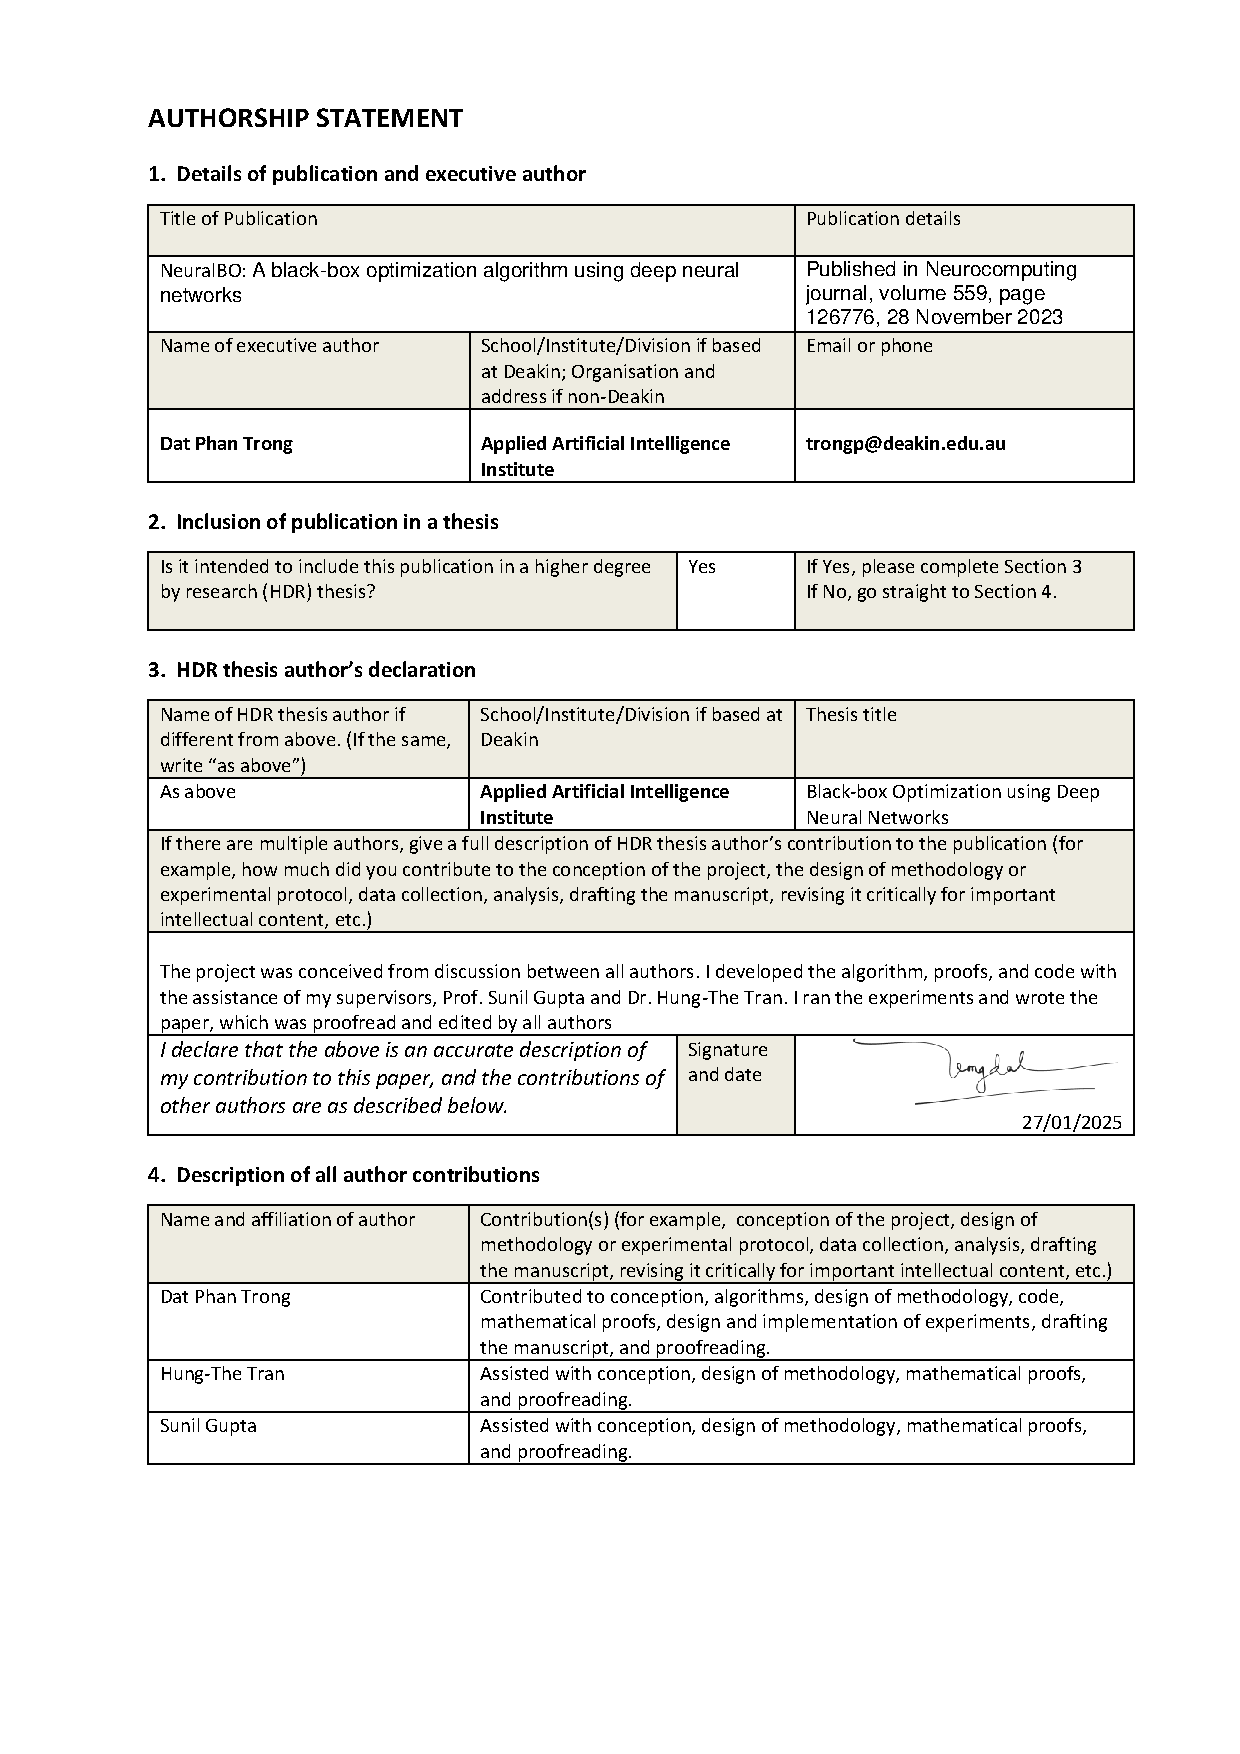
\includepdf[pages=-]{extra_pages/neuralbo_authorship_statement.pdf}

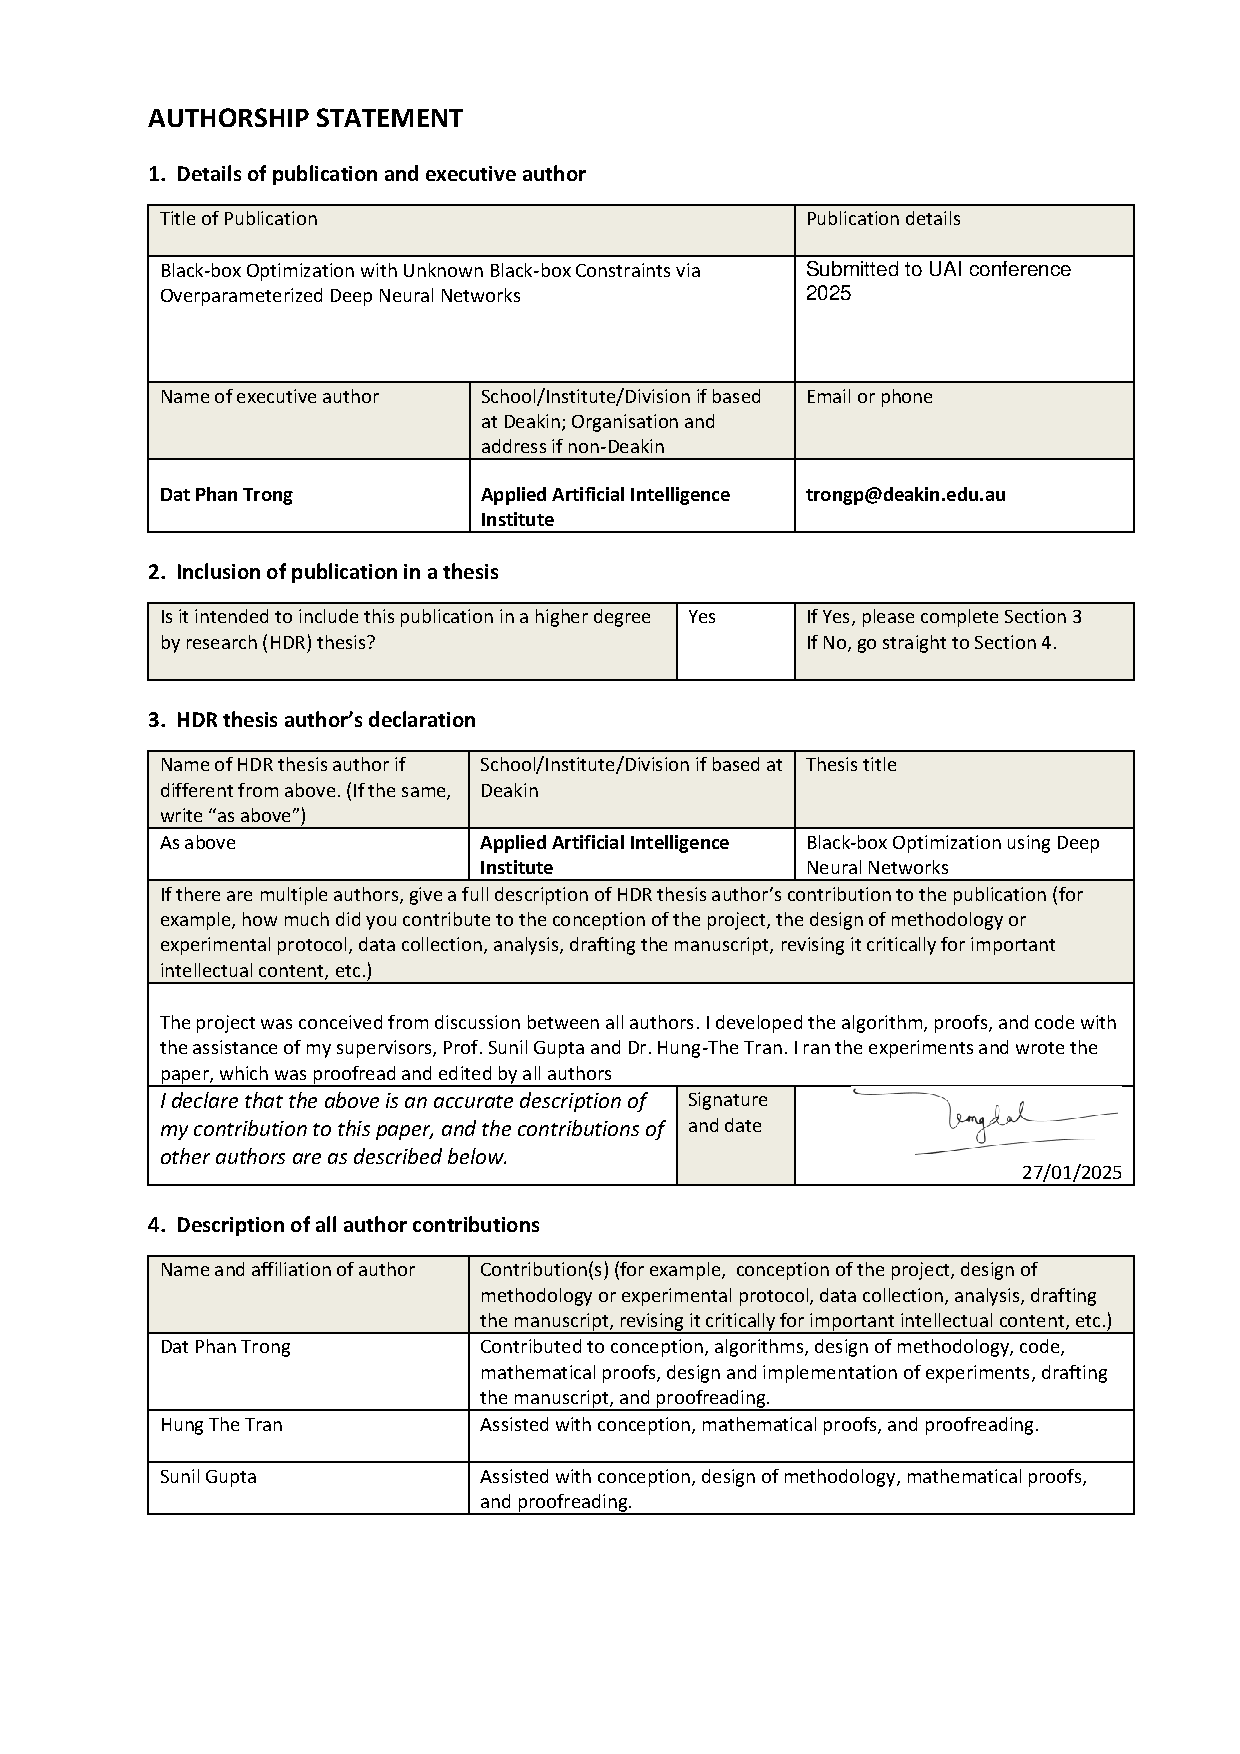
\includepdf[pages=-]{extra_pages/neural-cbo_authorship_statement.pdf}

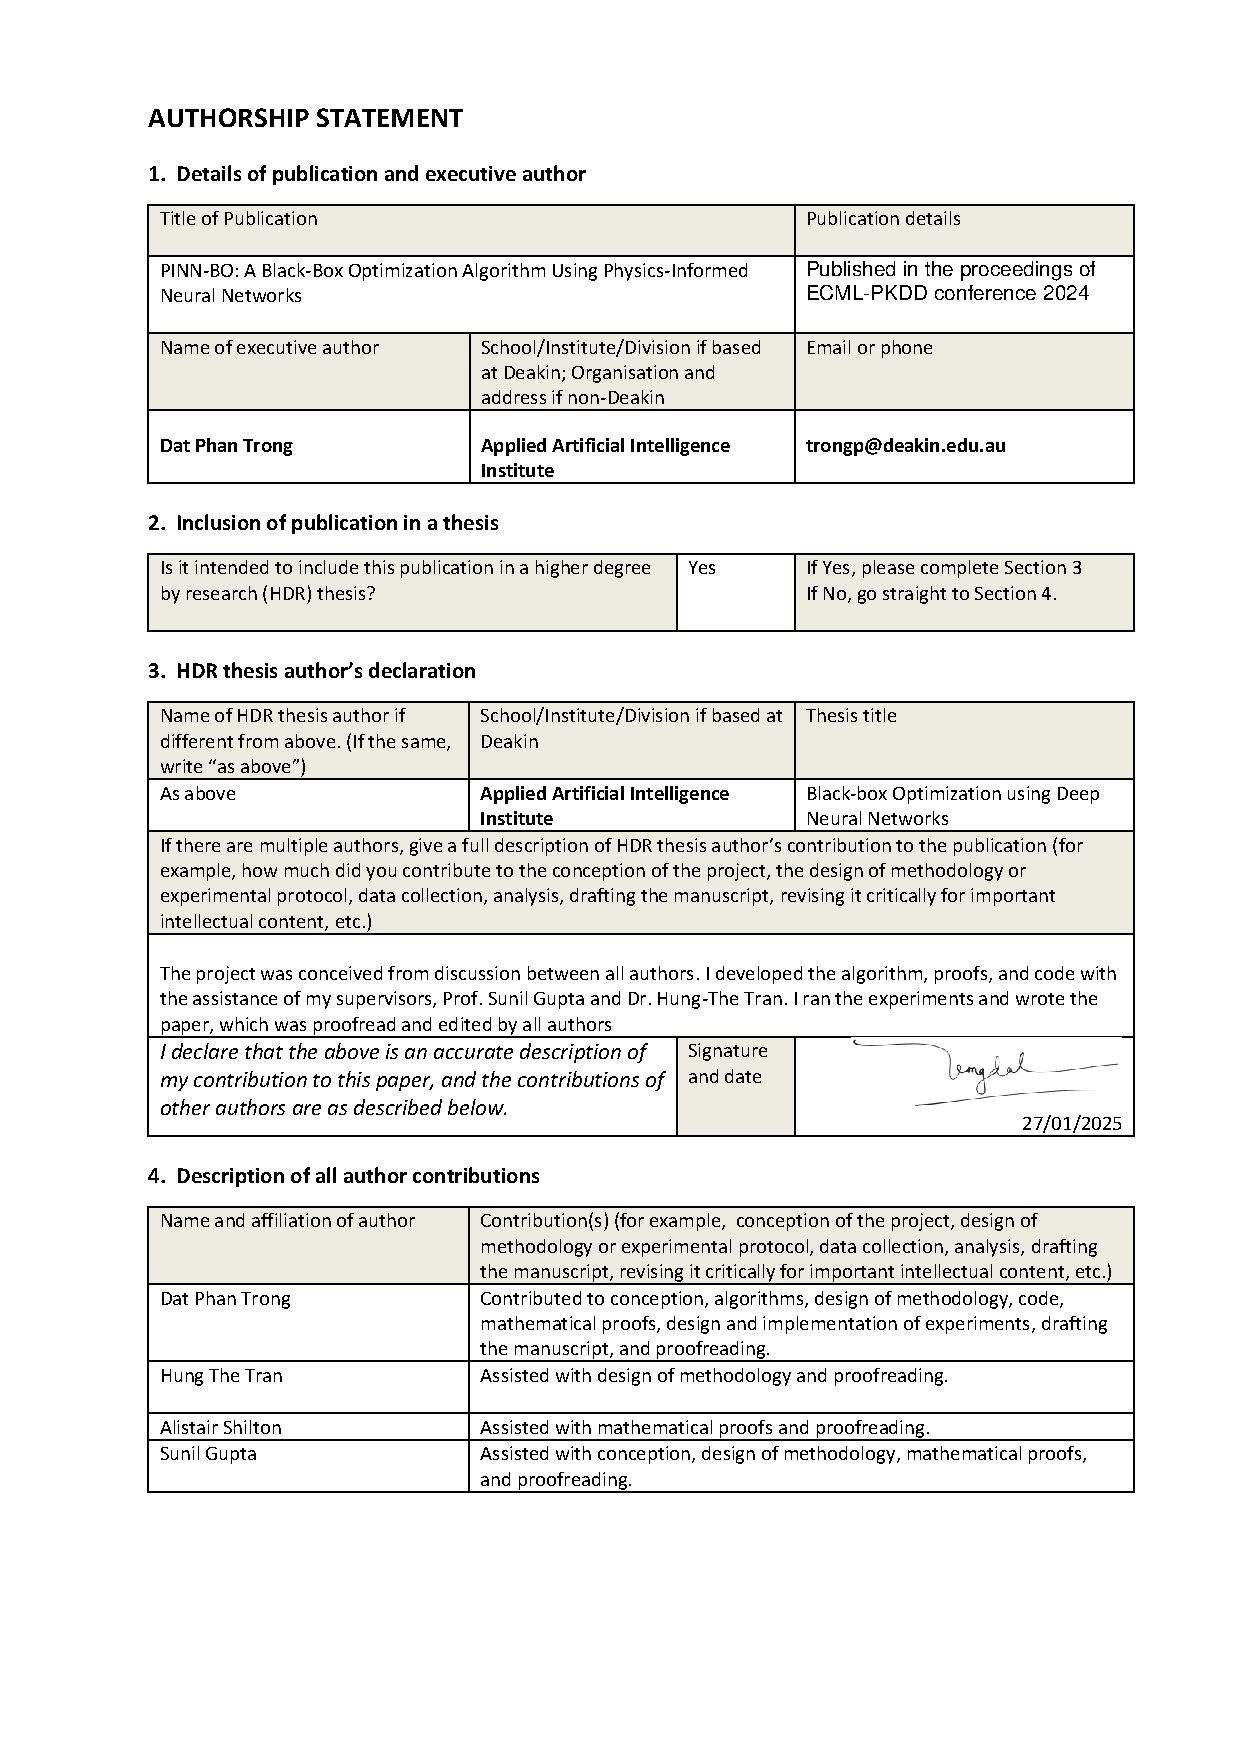
\includepdf[pages=-]{extra_pages/pinnbo_authorship_statement.pdf}
\cleardoublepage


%----------------------------------------------------------------------------------------
%	QUOTATION PAGE
%----------------------------------------------------------------------------------------

% \vspace*{0.2\textheight}

% \noindent\enquote{\itshape Thanks to my solid academic training, today I can write hundreds of words on virtually any topic without possessing a shred of information, which is how I got a good job in journalism.}\bigbreak

% \hfill Dave Barry

%----------------------------------------------------------------------------------------
%	ABSTRACT PAGE
%----------------------------------------------------------------------------------------

% \begin{abstract}
% \addchaptertocentry{\abstractname} % 


% \end{abstract}

%----------------------------------------------------------------------------------------
%	ACKNOWLEDGEMENTS
%----------------------------------------------------------------------------------------

\chapter*{Acknowledgements}
\phantomsection
\addcontentsline{toc}{chapter}{Acknowledgements}
\vspace*{\fill}
\noindent This thesis would not have been possible without the support, guidance, and encouragement of many people.

First, I would like to express my deepest gratitude to my primary supervisor, Prof. Sunil Gupta. His expertise, patience, and thoughtful advice have been essential during this journey. I am also sincerely thankful to my co-supervisor, Dr. Hung-The Tran, for his valuable insights, constructive feedback, and constant support, which have greatly improved my work.

I am especially grateful to Dr. Alistair Shilton for his important contributions to my physics informed black-box optimization project. His guidance and suggestions have helped me refine my ideas and approach. I also appreciate the time he dedicated to carefully reviewing this thesis.

I want to thank my friends and colleagues at the Applied Artificial Intelligence Institute (A\textsuperscript{2}I\textsuperscript{2}) for creating such a welcoming and supportive environment. Their encouragement and collaboration have made this experience both rewarding and enjoyable.

Lastly, I am deeply thankful to my family—my parents, my brother, and my partner. Their love, belief in me, and constant support have been my greatest source of strength. They have stood by me through every challenge and celebrated every achievement, and this thesis would not have been completed without them.

To everyone who has supported me along the way, I extend my heartfelt thanks. Your kindness and encouragement mean more to me than words can express.
\vspace*{\fill}
\cleardoublepage
\pagestyle{plain}


%----------------------------------------------------------------------------------------
%	LIST OF PUBLICATIONS
\chapter*{Relevant Publications}
\phantomsection
\addcontentsline{toc}{chapter}{Relevant Publications}
Parts of this thesis have been published elsewhere. The detail of these publications are as follows:

\begin{enumerate}
    \item \textit{Chapter \ref{chap:neural-bo}}: Phan-Trong, D., Tran-The, H., \& Gupta, S. (2023). NeuralBO: A black-box optimization algorithm using deep neural networks. Neurocomputing, 559, 126776.
    \item \textit{Chapter \ref{chap:neural-cbo}}: Phan-Trong, D., Tran, H. T., \& Gupta, S. (2024). Black-box Optimization with Unknown Black-box Constraints via Overparametrized Deep Neural Networks. Submitted to AISTATS 2025.  
    \item \textit{Chapter \ref{chap:pinn-bo}}: Phan-Trong, D., Tran, H. T., Shilton, A., \& Gupta, S. (2024, August). PINN-BO: A Black-Box Optimization Algorithm Using Physics-Informed Neural Networks. In Joint European Conference on Machine Learning and Knowledge Discovery in Databases (pp. 357-374). Cham: Springer Nature Switzerland.
    
\end{enumerate}
%----------------------------------------------------------------------------------------


%----------------------------------------------------------------------------------------
%	LIST OF CONTENTS/FIGURES/TABLES PAGES
%----------------------------------------------------------------------------------------
\hypersetup{linkcolor=black}
\pagenumbering{roman}
\tableofcontents % Prints the main table of contents

\listoffigures % Prints the list of figures

\listoftables % Prints the list of tables

\cleardoublepage
%\thispagestyle{plain}
%\chaptermark{Abbreviation}
\addcontentsline{toc}{chapter}{Abbreviations} \noindent
%\renewcommand{\nomname}{List of Abbreviations}

%--- Acronyms -----------------------------------------------------------------%
% \acrodef{label}[acronym]{written out form} % acronym syntax
%\acrodef{etacar}[$\eta$ Car]{Eta Carinae}   % acronym example
%--- Acronyms -----------------------------------------------------------------%
% how to use acronyms:
% \ac = use acronym, first time write both, full name and acronym
% \acf = use full name (text + acronym)
% \acs = only use acronym
% \acl = only use long text
% \acp, acfp, acsp, aclp = use plural form for acronym (append 's')
% \acsu, aclu = write + mark as used
% \acfi = write full name in italics and acronym in normal style
% \acused = mark acronym as used
% \acfip = full, emphasized, plural, used
%--- Acronyms -----------------------------------------------------------------%

\chapter*{List of Abbreviations}
\begin{multicols}{2}
\begin{acronym}
        \acro{bo}[BO]{Black-box Optimization}
        \acro{dnn}[DNN]{Deep Neural Network}
        \acro{ei}[EI]{Expected Improvement}
        \acro{es}[ES]{Entropy Search}
        \acro{pes}[PES]{Predictive Entropy Search}
        \acro{mes}[MES]{Max-value Entropy Search}
        \acro{kg}[KG]{Knowledge Gradient}
        \acro{gp}[GP]{Gaussian Process}
        \acrodefplural{gp}{Gaussian Processes}
        \acro{lcb}[LCB]{Lower Confidence Bound}
        \acro{ntk}[NTK]{Neural Tangent Kernel}
        \acro{rkhs}[RKHS]{Reproducing Kernel Hilbert Space}
        \acro{pde}[PDE]{Partial Differential Equation}
        \acro{pinn}[PINN]{Physics-Informed Neural Network}
        \acro{ts}[TS]{Thompson Sampling}
        \acro{ucb}[UCB]{Upper Confidence Bound}
        \acro{rf}[RF]{Random Forest}
        \acro{bnn}[BNN]{Bayesian Neural Network}
        \acro{deepgp}[Deep GP]{Deep Gaussian Process}
        \acro{mig}[MIG]{Maximum Information Gain}
        \acro{relu}[ReLU]{Rectified Linear Unit}
        \acro{PI}[PI]{Probability of Improvement}
        \acro{cdf}[CDF]{Cumulative Distribution Function}
        \acro{pdf}[PDF]{Probability Density Function}
        \acro{mab}[MAB]{Multi-armed Bandit}
\end{acronym}
\end{multicols}

%----------------------------------------------------------------------------------------
%	ABBREVIATIONS
%----------------------------------------------------------------------------------------


% \begin{abbreviations}{ll} % Include a list of abbreviations (a table of two columns)


% \textbf{LAH} & \textbf{L}ist \textbf{A}bbreviations \textbf{H}ere\\
% \textbf{WSF} & \textbf{W}hat (it) \textbf{S}tands \textbf{F}or\\

% \end{abbreviations}

%----------------------------------------------------------------------------------------
%	PHYSICAL CONSTANTS/OTHER DEFINITIONS
%----------------------------------------------------------------------------------------

% \begin{constants}{lr@{${}={}$}l} % The list of physical constants is a three column table

% % The \SI{}{} command is provided by the siunitx package, see its documentation for instructions on how to use it

% Speed of Light & $c_{0}$ & \SI{2.99792458e8}{\meter\per\second} (exact)\\
% %Constant Name & $Symbol$ & $Constant Value$ with units\\

% \end{constants}

%----------------------------------------------------------------------------------------
%	SYMBOLS
%----------------------------------------------------------------------------------------

% \begin{symbols}{lll} % Include a list of Symbols (a three column table)

% $a$ & distance & \si{\meter} \\
% $P$ & power & \si{\watt} (\si{\joule\per\second}) \\
%Symbol & Name & Unit \\

% \addlinespace % Gap to separate the Roman symbols from the Greek

% $\omega$ & angular frequency & \si{\radian} \\

% \end{symbols}

%----------------------------------------------------------------------------------------
%	DEDICATION
%----------------------------------------------------------------------------------------

% \dedicatory{For/Dedicated to/To my\ldots} 

%----------------------------------------------------------------------------------------
%	THESIS CONTENT - CHAPTERS
%----------------------------------------------------------------------------------------

\mainmatter % Begin numeric (1,2,3...) page numbering

\pagestyle{thesis} % Return the page headers back to the "thesis" style

% Include the chapters of the thesis as separate files from the Chapters folder
% Uncomment the lines as you write the chapters
\sloppy

\chapter*{Abstract} % Main chapter title
\addcontentsline{toc}{chapter}{Abstract}
\label{chap:abstract}
Optimization has become an essential task across numerous fields, as many systems and processes require fine-tuning to achieve maximum efficiency. In many cases, these systems are ``black-box'', meaning that the underlying mechanisms are unknown or too complex to model explicitly; we can only provide inputs and observe the resulting outputs. The challenge with optimizing black-box systems is that evaluating them can often be costly, both in terms of time and resources. This creates a demand for optimization methods that are not only effective but also sample-efficient, minimizing the number of evaluations needed to find optimal solutions. 


Bayesian optimization or \ac{bo} has emerged as a leading framework for optimizing expensive and unknown functions in various fields, including materials science, biomedical research, and machine learning. BO typically relies on two core components: (1) a surrogate model that approximates the underlying function based on available observations, and (2) an acquisition function that balances the trade-off between exploration (searching unexplored regions with high uncertainty) and exploitation (refining known promising regions). Traditionally, \ac{gp} has been the preferred choice for the surrogate model due to its ability to quantify uncertainty and its analytic expression, hence being convenient to provide theoretical guarantees. However, \acp{gp} suffer from cubic computational complexity in relation to the number of observations, making them impractical for large-scale applications.


First of all, investigating alternative surrogate models to enhance the performance of standard \ac{bo}, especially in scenarios where \ac{gp} are computationally prohibitive, is focused. 
The ability of \acp{dnn} to scale linearly with the number of data points and capture complex patterns makes them more suitable for tasks involving structural data (like images and text). We introduce \textbf{Neural-BO}, a \ac{dnn}-based optimization algorithm that leverages recent advances in neural network theory to estimate uncertainty and uses \ac{ts} for next point selection. This method maintains the flexibility of \acp{dnn} while achieving convergence guarantees through the \ac{ntk}-based theory, showing improved sample efficiency and faster convergence.   

However, optimizing real-world functions often goes beyond simple maximization or minimization, requiring the incorporation of constraints. These constraints ensure that solutions not only optimize the objective but also meet critical feasibility criteria, which is especially important in domains like engineering and physics. Hence, we extend the \ac{dnn}-based approach to handle optimization problems with expensive, unknown constraints through \textbf{Neural-CBO}. In this method, both the objective function and the constraints are modeled using DNNs, and the acquisition function is designed to balance exploration and exploitation while ensuring constraint satisfaction. By using \ac{lcb} conditions to guarantee feasibility and the \ac{ei} acquisition function to guide the search, Neural-CBO efficiently explores the feasible region, even when it is significantly smaller than the overall search space. Our method provides upper bounds on both regret and constraint violations, offering a theoretically sound and scalable approach for constrained black-box optimization tasks.

Moreover, in fields like physics, engineering, and biology, there is often domain-specific knowledge available, typically in the form of physical laws or models, which can be expressed as \acp{pde}. Incorporating physical knowledge into the optimization process enhances function approximation by providing more accurate guidance, improving surrogate model predictions, and reducing uncertainty in regions that follow known physical laws. Therefore, we propose PINN-BO, an approach that integrates \ac{pinn} into the \ac{bo} framework.  By incorporating these physical constraints into the optimization process, PINN-BO significantly improves sample efficiency. The method employs \ac{pinn} to model the objective function, utilizing known physical principles by embedding the \ac{pde} into the network's training process. This ensures that the optimization process not only converges quickly but also remains aligned with the underlying physical system. Experimental results on both synthetic and real-world tasks demonstrate the superior performance of PINN-BO in domains where physical knowledge is crucial. 

In summary, this thesis proposed three novel methods, each leveraging \acp{dnn}-based surrogate models to enhance computation complexity and sample efficiency in \ac{bo} as well as its extended settings.

% \paragraph{\huge List of Publications}
% \begin{enumerate}
%     \item Phan-Trong, D., Tran-The, H., \& Gupta, S. (2023). NeuralBO: A black-box optimization algorithm using deep neural networks. Neurocomputing, 559, 126776.
%     \item Phan-Trong, D., Tran, H. T., Shilton, A., \& Gupta, S. (2024, August). PINN-BO: A Black-Box Optimization Algorithm Using Physics-Informed Neural Networks. In Joint European Conference on Machine Learning and Knowledge Discovery in Databases (pp. 357-374). Cham: Springer Nature Switzerland.
%     \item Phan-Trong, D., Tran, H. T., \& Gupta, S. (2024). Black-box Optimization with Unknown Black-box Constraints via Overparametrized Deep Neural Networks. Submitted to AISTATS 2025.  
% \end{enumerate}


\chapter{Introduction} % Main chapter title

\label{chap:introduction} % For referencing the chapter elsewhere, use \ref{Chapter1} 

%----------------------------------------------------------------------------------------

% Define some commands to keep the formatting separated from the content 
\newcommand{\keyword}[1]{\textbf{#1}}
\newcommand{\tabhead}[1]{\textbf{#1}}
\newcommand{\code}[1]{\texttt{#1}}
\newcommand{\file}[1]{\texttt{\bfseries#1}}
\newcommand{\option}[1]{\texttt{\itshape#1}}

Science has made a great impact on society. From healthcare to food production to modern communication, scientific breakthroughs have transformed nearly every facet of human life. Many of these breakthroughs arise from experiments conducted on complex, unknown systems, with the aim of discovering which inputs yield the most favorable outputs. Some well-known examples are the synthesis of short polymer fiber materials, alloy design, 3D bio-printing, molecule design, etc., \citep{greenhill2020bayesian, shahriari2015taking}. In many cases, experts rely on informed guesses or prior knowledge to decide which inputs to test. This trial-and-error process typically requires numerous experiments to identify the optimal input, a task that can be both time-consuming and expensive. The high costs, in terms of both financial resources and labor, restrict the extent to which these systems can be optimized, thereby slowing progress in research and industry. Therefore, strategies that help find optimal solutions with fewer trials could significantly speed up innovation.

Bayesian Optimization is one of the most effective methods for optimizing expensive, black-box systems \citep{mockus1978application, streltsov1999non}. It works by using all previous inputs and their corresponding outputs, along with any known information about the system, to build a statistical model of the function. Typically, a probabilistic model such as a \acf{gp} is trained on available observations. This model helps generate an acquisition function that balances exploration (trying new inputs) and exploitation (refining known good inputs). The acquisition function is optimized to suggest the next input to evaluate, and the resulting output is used to update the model. By iterating this process, Bayesian Optimization can identify optimal inputs with far fewer experiments than traditional methods, leading to significant cost savings in both time and resources. 

Mathematically, we can formalize this task as a global optimization problem to optimize $f(\mathbf{x})$ subject to $\mathbf{x} \in \mathcal D \subset \mathbb{R}^d$, where $d$ is the number of dimensions, and $f$ is an expensive black-box system that can only be evaluated point-wise. Further, due to various reasons (e.g., imperfect measurements), we often only have access to noisy evaluations of $f$ in the form $y = f(\mathbf{x}) + \epsilon$, where $\epsilon$ is the noise.

Bayesian Optimization has found widespread use across various disciplines, including materials science, biomedical research, and even other areas of computer science. In materials science, it has contributed to innovations such as the creation of new polymer fibers \citep{li2017rapid}, the analysis of metal oxide grain boundary structures \citep{kikuchi2018bayesian}, and the enhancement of thermal conductivity in nanostructures \citep{ju2017designing}. Within biomedical research, it has been applied to a range of tasks, such as aiding in COVID-19 diagnosis \citep{nour2020novel}, examining the impact of aging on time perception \citep{turgeon2016cognitive}, and designing synthetic genes \citep{gonzalez2015bayesian}. In computer science, Bayesian optimization is frequently utilized to improve robot control \citep{berkenkamp2023bayesian} and fine-tune hyperparameters in machine learning models \citep{snoek2012practical,bergstra2012random}.

A key component in Bayesian Optimization is the \textit{surrogate model}. As an approximation of the true objective function, the surrogate model provides both predictions of the function’s value and estimates of uncertainty for each potential input. This dual output is crucial for designing the acquisition function, which determines the next point to sample in the optimization process. The acquisition function uses the surrogate model's predictions to balance exploration and exploitation. Exploration encourages sampling in regions with high uncertainty, where the model is less confident, in the hope of discovering better solutions. Exploitation, on the other hand, focuses on regions where the surrogate predicts high performance, aiming to refine promising areas. By leveraging the surrogate model's predictions and uncertainty estimates, the acquisition function can suggest new inputs that strategically advance the search for the optimal solution, while minimizing the number of expensive evaluations required.

Due to their flexibility, well-calibrated uncertainty estimates, and favorable analytical properties, \ac{gp} has long been a popular choice for modeling distributions over functions in Bayesian Optimization \citep{osborne2009gaussian}. \ac{gp} provides a probabilistic framework that captures not only the predictions of the objective function, but also the uncertainty associated with those predictions, allowing Bayesian optimization to balance exploration and exploitation effectively. Additionally, the ability of \ac{gp} to compute closed-form posterior distributions and acquisition functions, such as \ac{ei} or \ac{ucb}, further enhances its appeal for efficient decision-making in optimization tasks. The combination of Bayesian Optimization with \ac{gp} has led to strong theoretical results, particularly in terms of convergence guarantees. For instance, \citet{srinivas2009gaussian} presented rigorous theoretical bounds showing that Bayesian Optimization with GP models can achieve sublinear regret, which means that the performance of the algorithm improves efficiently over time as more data is gathered. Moreover, this framework has been successfully extended to more complex settings, including multitask and multi-objective optimization \citep{swersky2013multi}, where \ac{gp} can jointly model several related tasks or objectives, leveraging shared information to improve optimization efficiency across different tasks.

Despite these advantages, \ac{gp} comes with inherent limitations that have motivated further research into alternative models. One major challenge is the computational complexity associated with \ac{gp}, particularly the cubic time complexity for inference, which becomes prohibitive as the dataset (i.e. the set of function evaluations gathered during the optimization process) grows. This computational burden is especially problematic when handling large-scale problems or high-dimensional input spaces, where \ac{gp} struggles due to the curse of dimensionality. 
While \ac{gp} remains the dominant choice for modeling in Bayesian optimization, in response to these challenges,  researchers are actively exploring more alternative models to \ac{gp}, such as \ac{rf}, \ac{bnn}, and \ac{deepgp}. These models aim to retain some of the desirable properties of \ac{gp}, such as uncertainty quantification and flexibility while improving scalability and performance in high-dimensional spaces. For instance, \acfp{rf} and \acfp{dnn} have been employed to estimate black-box functions in this context. \acp{rf} tend to perform well at making accurate predictions in the vicinity of the training data. However, they struggle with extrapolation, meaning their performance can significantly deteriorate when making predictions outside the range of observed data points \citep{shahriari2015taking}. Additionally, hybrid approaches that combine \ac{gp} with other models or approximate inference techniques, such as variational methods \citep{tran2016variational} and sparse approximations \citep{snelson2007local}, are being developed to tackle the computational bottlenecks and extend the practical applicability of \ac{gp} and Bayesian Optimization to more complex and large-scale problems.  The first significant application of \ac{dnn} in Bayesian Optimization was introduced by \citet{snoek2015scalable}, who employed a \ac{dnn} to transform high-dimensional inputs into lower-dimensional feature vectors. These feature vectors were then fitted to a Bayesian linear regression surrogate model, allowing for more efficient optimization. Another promising approach was presented in \citet{springenberg2016bayesian}, where the objective function was modeled directly using a \acf{bnn}. This method aimed to capture the complex relationships within the data while providing uncertainty estimates for the predictions. Despite the empirical success of these neural network approaches in Bayesian optimization tasks, a significant gap remains in the theoretical understanding of their convergence properties. Unlike \acp{gp}, which have well-established theoretical frameworks demonstrating their convergence guarantees, the algorithms leveraging neural networks lack similar assurances. This absence of theoretical backing raises questions about the reliability and robustness of these methods in practice, particularly in high-dimensional applications. Moreover, the use of Bayesian linear regression or \acp{bnn} introduces substantial computational challenges. Both approaches require maintaining an ensemble of models to derive the posterior distribution over the parameters, leading to increased complexity and potentially prohibitive computational costs. As the dimensionality of the input space or the size of the dataset grows, the demand for computational resources can become a critical limitation. Consequently, while alternative models like random forests and neural networks present exciting avenues for exploration in Bayesian optimization, further research is \textit{necessary to develop} methods that not only demonstrate empirical efficacy but also provide the theoretical guarantees and computational efficiency needed for practical application.

Real-world optimization problems often come with \textit{unknown constraints}. In this setting, black-box optimization with black-box constraints becomes crucial, as both the objective function and constraints need to be optimized simultaneously while ensuring that evaluations are made within feasible regions. Traditional \ac{bo} methods, which focus solely on optimizing the objective function, fail to capture the interplay between the unknown constraints and the objective, potentially leading to infeasible or suboptimal solutions. Hence, considering only standard \ac{bo} is insufficient to address such tasks effectively. Many attempts have been made to tackle this challenge by incorporating constraint handling into the \ac{bo} framework, resulting in methods specifically designed for constrained \ac{bo} \citep{gelbart2014bayesian, ariafar2019admmbo, nguyen2023optimistic}. However, despite these advancements, all of these methods still rely on \acp{gp} as the surrogate model, which introduces drawbacks similar to those seen in standard \ac{gp}-based \ac{bo}, such as poor scalability and increasing computational costs as the number of observations grows. This limitation motivates further \textit{exploration} into more scalable surrogate models, such as \acp{dnn}, to better handle the complexities of black-box optimization with black-box constraints.

In many scientific and engineering domains, the objective function and its constraints are governed by well-established physical principles, such as conservation laws, thermodynamics, or fluid dynamics. These principles can often be expressed in the form of \acp{pde} or other mathematical models that describe the underlying system behavior. \textit{Integrating this prior knowledge into the \ac{bo} framework can significantly improve both the efficiency and accuracy of the optimization process}. By leveraging physical knowledge, we not only reduce the need for expensive function evaluations but also ensure that the optimization process remains within physically feasible regions, thereby avoiding solutions that violate fundamental laws. Following these motivations, we introduce our main aims and approaches.


\section{Aims and Approaches}
The main objective of this thesis is to improve the performance and scalability of \acl{bo}, especially on structural data.  More specifically, we focus on these aims:
\begin{enumerate}[label= Aim \arabic*, align=left]
    \item As the number of optimization iterations increases, \acp{gp}-based black-box optimization faces computational costs, leading to poor scalability. To address this, we aim to develop a scalable BO method replacing the traditional \ac{gp} surrogate model with a more scalable alternative - \ac{dnn}. \label{aim:1}
    \item We aim to use \ac{dnn} surrogate models into black-box optimization with black-box, expensive constraints.  \label{aim:2}
    \item We aim to improve the performance of black-box optimization by integrating useful physical information in the form of \acfp{pde}. \label{aim:3}
\end{enumerate}
To realize these aims, we have developed \ac{dnn}-based methods that are both computationally efficient, scalable and come with rigorous theoretical guarantees on their sample efficiency. We briefly summarize them below:
\begin{itemize}
    \item To achieve \ref{aim:1}, we replace the conventional \ac{gp} model by a \ac{dnn} surrogate model. We propose a novel a \acl{ts} based strategy for choosing the next evaluation. We name this method as Neural-BO.
    \item To achieve \ref{aim:2}, we construct an \acf{ei} acquisition function to select the next samples within a feasible region, determined by \acf{lcb} conditions for all constraints. The \acs{lcb}-based approach guarantees constraint feasibility, while \acs{ei} efficiently balances exploration and exploitation, especially when the region is significantly smaller than the overall search space. We call this method as Neural-CBO.
    \item To achieve \ref{aim:3}, we model the objective function using a \acf{pinn}. By incorporating physical knowledge, expressed through \acp{pde}, into the \ac{pinn} training process, we enhance the sample efficiency of the black-box optimization.  We call this method PINN-BO. 
\end{itemize}
\section{Significant Contributions}
The work presented in this thesis is important as it addresses the scalability limitations found in \acp{gp}-based \acf{bo}. As \ac{bo} is often used in expensive problem settings, our approach significantly lowers both the computational and experimental cost across a wide range of practical tasks. Specifically: 
\begin{itemize}
    \item As \acp{gp} scale poorly with the number of data points, \ac{gp}-based \ac{bo} have to deal with the increasing computational cost when the number of optimization iterations increases. \acp{dnn}-based approaches, such as methods, that rely on \acp{bnn} to manage predictive uncertainty, continue to face computational challenges. Our Neural-BO algorithm, in contrast,  incorporates recent advances in neural network theory through the use of \ac{ntk} to estimate a confidence interval around the neural network model and employs a \acl{ts} technique to determine the next evaluation point. Our theoretical analysis of the NeuralBO's regret bound demonstrates that it is both convergent and more sample-efficient than existing \ac{gp}-based methods. Furthermore, we show the potential of our Neural-BO algorithm in optimizing complex structured data, such as images and text, while maintaining a computational complexity that only grows linearly with the number of data points. The experimental results on synthetic benchmarks and real-world optimization tasks highlight that our algorithm outperforms the current state-of-the-art in \ac{bo}.  
    \item In real-world situations, \ac{bo} tasks often come along with unknown, expensive constraints. Our Neural-CBO has extended the \ac{dnn}-based idea to this unknown, expensive constraints \ac{bo} problem. By inheriting the good scalability of \acp{dnn},  we modeled both the objective function and constraints using \acp{dnn}, and used \ac{ei} as the acquisition function. The feasible region is determined using \ac{lcb} conditions, ensuring constraint satisfaction while balancing exploration and exploitation. Our theoretical analysis shows that cumulative regret and constraint violations have upper bounds comparable to Gaussian Process-based methods. Benchmarking experiments on synthetic and real-world tasks demonstrate that Neural-CBO performs competitively with state-of-the-art techniques. 
    \item We focus on a \ac{bo} problem, where the black-box function is governed by physical laws through \acp{pde}. To address this, we introduce the PINN-BO algorithm, which offers several advantages: enhanced sample efficiency in optimization, scalable computation that grows linearly with the number of function evaluations, and the ability to handle a wide variety of \acp{pde}. We theoretically analyse our algorithm and prove that its regret bound is tighter than the case when PDE information is not utilized. We empirically demonstarte that PINN-BO outperforms existing methods that do not incorporate physical knowledge across both synthetic and real-world problems. 
\end{itemize}

\section{Structure of this Thesis}
\begin{itemize}
    \item Chapter \ref{chap:background} provides a background and discussion of the related works relevant to this thesis. We begin by introducing the optimization problem and its variants,  from gradient-based approaches to derivative-free strategies under black-box assumptions on the objective functions. Then we describe black-box optimization and its core components, including surrogate models and acquisition functions. We discuss various surrogate models, such as \acp{gp} with their associated kernels, and \acp{dnn}, particularly in over-parameterized settings, highlighting their reliance on key mathematical tools. We then link these models through the lens of \ac{rkhs}. Next, we introduce the trade-off between exploration-exploitation through acquisition functions, with a focus on utility-based acquisition functions (e.g., \ac{ts}, \ac{ei}, and \ac{ucb}). Additionally, we discuss other types of acquisition functions, such as those based on information theory (\ac{es}, \ac{pes}, \ac{mes}). We also discuss Bandit-based Optimization and establish a connection with Black-box Optimization. Finally, we conclude with the open problems that guide the work carried out in this thesis.  
    \item Chapter \ref{chap:neural-bo} presents our \ac{dnn}-based black-box optimization method named Neural-BO. We begin by discussing the motivations behind the approach and explain how to mathematically integrate a \ac{dnn} model with \acl{ts}. Next, we present the theoretical analysis (regret bound) for our proposed method under regular assumptions.  Finally, we provide experimental results on both real-world and synthetic optimization problems, demonstrating that our method outperforms current approaches, especially in high-dimensional structural data.  
    \item Chapter \ref{chap:neural-cbo} presents the Neural-CBO method, which utilizes the benefit of \ac{dnn}-based surrogate model into black-box optimization under unknown, black-box constraints. We detail how to use \ac{dnn} to model, control the uncertainty and balance the exploration-exploitation of both objective function and constraints. Finally, we provide a theoretical guarantee for not only  the cumulative regret of the objective function but also for the constraint violation. Similar to Chapter \ref{chap:neural-bo}, we conduct a wide range of experiments, from synthetic to real-world benchmarks, to demonstrate the effectiveness of our method.     
    \item Chapter \ref{chap:pinn-bo} presents the PINN-BO method, which addresses optimization problems where the objective function is governed by physical knowledge, expressed as \acp{pde}. We begin by presenting our optimization problem setting involving the PDEs. We next describe various components of our efficient optimization algorithm PINN-BO. We then provide a theoretical analysis of the convergence of PINN-BO leveraging the properties of \ac{pinn} under \ac{ntk} perspective.
    \item Chapter \ref{chap:conclusion} concludes this thesis with a summary of our contributions and a discussion of potential future works.
\end{itemize}

\chapter{Background} % Main chapter title

\label{chap:background} 

% Define some commands to keep the formatting separated from the content 
This chapter provides a structured exploration of black-box optimization, beginning with the basic mathematical concepts necessary for understanding the subject. Section \ref{section:math_backgrounds} introduces the fundamental mathematical tools and principles that support optimization theory, ensuring a solid foundation for later discussions. Section \ref{section:optimization_introduction} provides a general overview of optimization, distinguishing between local and global approaches and highlighting their respective roles and applications.

In Section \ref{section:black_box_optimization}, we shift our focus to black-box optimization, examining the challenges posed by functions that are expensive to evaluate or lack explicit mathematical representation. Section \ref{section:bo_unknown_constraints} extends this discussion by addressing problems with unknown constraints, emphasizing strategies to effectively explore feasible regions in such complex scenarios. Section \ref{section:bo_physics} explores how incorporating physics-based knowledge into optimization frameworks can improve both solution accuracy and computational efficiency. Finally, in Section \ref{section:bo_further_research}, we conclude the chapter by outlining potential future research directions, focusing on unresolved challenges and emerging opportunities in black-box optimization.

\section{Essential Mathematics Backgrounds}
\label{section:math_backgrounds}
\subsection{Gaussian and Sub-Gaussian Random Variables}
\subsubsection{Gaussian Random Variables}  
Gaussian random variables, also known as normal random variables, are fundamental in probability theory and statistics. A Gaussian random variable \( X \) is fully characterized by its mean \( \mu \) and variance \( \sigma^2 \), and its probability density function (PDF) is given by:  
\[
f_X(x) = \frac{1}{\sqrt{2\pi \sigma^2}} \exp\left(-\frac{(x - \mu)^2}{2\sigma^2}\right), \quad x \in \mathbb{R}.
\]  
The tails of a Gaussian distribution decay exponentially, meaning the probability of large deviations from the mean diminishes rapidly. Specifically, for \( X \sim \mathcal{N}(\mu, \sigma^2) \), the tail probability can be bounded as:  
\[
\mathbb{P}(|X - \mu| > t) \leq 2 \exp\left(-\frac{t^2}{2\sigma^2}\right), \quad t > 0.
\]  

This exponential decay of tail probabilities is a key property that makes Gaussian distributions central to statistical theory and concentration inequalities. However, many random variables in practice exhibit similar tail behaviors without necessarily following the exact Gaussian distribution. This motivates the broader class of \textit{sub-Gaussian random variables}.  

\subsubsection{Sub-Gaussian Random Variables}  
A random variable \( X \) is sub-Gaussian if its tail probabilities decay at least as fast as those of a Gaussian random variable. Intuitively, sub-Gaussian random variables are those whose deviations from their mean are tightly controlled, similar to or better than the Gaussian case.  

Formally, \( X \) is sub-Gaussian if there exists a constant \( \sigma > 0 \) such that for all \( t > 0 \):  
\[
\mathbb{P}(|X - \mathbb{E}[X]| > t) \leq 2 \exp\left(-\frac{t^2}{2\sigma^2}\right).
\]  
Here, \( \sigma^2 \) is called the \textit{sub-Gaussian variance parameter}, and it provides a measure of the "spread" of the random variable, analogous to the variance in a Gaussian distribution.  

An equivalent definition involves the moment generating function (MGF). A random variable \( X \) is sub-Gaussian if there exists a constant \( \sigma > 0 \) such that:  
\[
\mathbb{E}[\exp(\lambda(X - \mathbb{E}[X]))] \leq \exp\left(\frac{\lambda^2 \sigma^2}{2}\right), \quad \forall \lambda \in \mathbb{R}.
\]  

Many common random variables exhibit sub-Gaussian behavior, including Gaussian, bounded, and discrete random variables. Below are some illustrative examples:  
\begin{itemize}
    \item \textbf{Gaussian Random Variables:} Any Gaussian random variable \( X \sim \mathcal{N}(\mu, \sigma^2) \) is inherently sub-Gaussian, with \( \sigma^2 \) as its variance.  
    \item \textbf{Bounded Random Variables:} If \( X \) is a bounded random variable, i.e., \( |X| \leq B \) almost surely, then \( X \) is sub-Gaussian with \( \sigma \leq B \).  
    \item \textbf{Rademacher Random Variables:} A Rademacher random variable, which takes values \( \pm 1 \) with equal probability, is sub-Gaussian with \( \sigma = 1 \).  
\end{itemize}  

Sub-Gaussian random variables exhibit several important properties that make them useful in probabilistic analyses, particularly when handling extreme deviations and ensuring concentration of measure. These properties include:  
\begin{itemize}
    \item \textbf{Tight Tail Bounds:} Sub-Gaussian random variables satisfy exponential tail bounds, making them useful in scenarios where extreme deviations must be controlled.  
    \item \textbf{Closed under Affine Transformations:} If \( X \) is sub-Gaussian, then \( aX + b \) is also sub-Gaussian, with the sub-Gaussian parameter scaled by \( |a| \).  
    \item \textbf{Sum of Independent Sub-Gaussians:} If \( X_1, X_2, \dots, X_n \) are independent sub-Gaussian random variables, their sum \( S_n = \sum_{i=1}^n X_i \) is also sub-Gaussian, with the variance parameter satisfying \( \sigma^2_{S_n} = \sum_{i=1}^n \sigma_i^2 \).  
\end{itemize} 

While sub-Gaussian random variables provide valuable tools for modeling uncertainties in single values, many real-world problems cannot be modeled with single values, as these problems often deal with the uncertainty over entire functions. Therefore, it becomes necessary to capture the dependencies between the values of the function at different locations or times, which implies a need for working with joint distributions. The key challenge arises when dealing with functions, which can take values at infinitely many points, thus requiring a notion of probability distributions over functions. In the next section,  we introduce \acf{gp}, which is the natural extension of the normal distribution from the case of individual random variables to function spaces.

\subsection{Gaussian Process}
\label{section:gaussian_process}
A \acf{gp} is a finite collection of normally distributed random variables with each having a multivariate normal distribution. \ac{gp} offers a prior distribution over smooth functions and are completely specified by a mean function, $\mu(\mathbf{x})$ and covariance function, $k(\mathbf{x}, \mathbf{x}^\prime)$. We have \begin{equation}
    \label{def:GP}
    f({\bf x})\sim\mathrm{GP}(\mu({\bf x}),k({\bf x},{\bf x}^\prime))
\end{equation}
where the mean and variance of a normal distribution is returned as the value of $f(\mathbf{x})$ for an arbitrary $\mathbf{x}$. Without loss in generality, $f(\mathbf{x})$ values can be assumed as a realization of random variables with prior mean as zero thus making the Gaussian process fully specified by the covariance matrix \citep{rasmussen2006gaussian}. There are many popular covariance functions including Mat\'ern kernel, Linear kernel, Squared Exponential kernel. These kernels will be briefly introduced in the next section.

% In that the Squared Exponential (SE) kernel is a popular choice.

% \begin{equation}
%      \left.k({\bf x},{\bf x}^{\prime}) = \exp (-\frac{1}{2 \ell^{2}} \norm{\bf x - \bf x^{\prime}}^{2}) \right.
% \end{equation}
% In the above kernel, $\ell$ is a length scale parameter related to the smoothness of the function. When $\mathbf{x}_i$ and $\mathbf{x}_j$
% values get close together, this function returns high value and else it returns value close to 0.
We assume that function values ${\mathbf{y}}_{1:t} = f(\mathbf{x}_{1:t})+\epsilon_{1:t}$ corresponding to the initial points $\mathbf{x}_{1:t}$ are sampled
from the prior Gaussian process. Collectively we denote the observations as $\mathcal{D}_{1:t} = \{\mathbf{x}_{1:t}, \mathbf{y}_{1:t}\}$. The function
values $f(\mathbf{x}_{1:t})$ follow a multivariate Gaussian distribution $\mathcal{N}(0, \mathbf{K}_t)$, where
\[ \mathbf{K}_t = \begin{bmatrix} 
    k(\mathbf{x}_1, \mathbf{x}_1) & \dots  & k(\mathbf{x}_1, \mathbf{x}_t)\\
    \vdots & \ddots & \vdots\\
    k(\mathbf{x}_t, \mathbf{x}_1) & \dots  & k(\mathbf{x}_t, \mathbf{x}_t)
    \end{bmatrix}
\]
Given a new point $\mathbf{x}_{t+1}$, then $\mathbf{x}_{t+1},  y_{1:t}$ and $f(\mathbf{x}_{t+1})$ are jointly Gaussian. By the properties of Gaussian process we
can write

\[
\begin{pmatrix}
\mathbf{y}_{1:t} \\
f(\mathbf{x}_{t+1})
\end{pmatrix} \sim \mathcal{N}\left(0, \begin{bmatrix}
\mathbf{K}_t & \mathbf{k}_{1:t} \\
\mathbf{k}_{1:t}^\top & k(\mathbf{x}_{t+1}, \mathbf{x}_{t+1})
\end{bmatrix} \right), 
\]
where $\mathbf{k}_{1:t} = \begin{bmatrix}
k(\mathbf{x}_{t+1}, \mathbf{x}_1) & k(\mathbf{x}_{t+1}, \mathbf{x}_2) & \dots & k(\mathbf{x}_{t+1}, \mathbf{x}_t)
\end{bmatrix}$.

Then using Sherman-Morrison-Woodbury formula in \citet{rasmussen2006gaussian}, the predictive distribution is:
\[ \mathbb{P}(y_{t+1} \lvert \mathcal{D}_{1:t}, \mathbf{x}_{t+1})= \mathcal{N}(\mu_t(\mathbf{x}_{t+1}), \sigma_t^2(\mathbf{x}_{t+1})), 
\]
where the predictive mean is $\mu_t(\mathbf{x}_{t+1}) = \mathbf{k}_{1:t}^\top \mathbf{K}_t^{-1} \mathbf{y}_{1:t}$ and variance $\sigma_{t}^{2}({\bf x}_{t+1}) = k({\bf x}_{t+1},{\bf x}_{t+1})-{\bf k}_{1:t}^{\top} \mathbf{K}_t^{-1}{\bf k}_{1:t}$. 

\subsection{Kernels}
\label{section:kernels}
In the context of \acfp{gp}, kernels (also known as covariance functions) play a crucial role in defining the prior belief about the function being modeled. A kernel, denoted as $k(\mathbf{x}, \mathbf{x}^\prime)$, quantifies the similarity or correlation between function values at two input locations, $\mathbf{x}$ and $\mathbf{x}^\prime$. It is symmetric, positive semi-definite, and it defines the properties of the functions sampled from the \ac{gp} prior. These properties ensure that the resulting covariance matrix constructed using this kernel will be valid (positive semi-definite), which is necessary for the Gaussian Process to be well-defined.

The choice of kernel is a critical aspect of \ac{gp} modeling, as it directly impacts the smoothness, complexity, and overall behavior of the functions that the model is capable of representing. Different kernels encode different assumptions about the underlying function we are attempting to model, and it is crucial to carefully consider these assumptions when choosing a kernel for a specific task. From the perspective of Bayesian inference, the kernel can be seen as the main source of prior information about the properties of the functions we are modeling. Therefore, it is essential to choose a kernel that is appropriate for the structure and characteristics that one might expect from the function. We now consider some common types of kernels, each with its own assumptions and characteristics:

\paragraph{Linear Kernel:}
The linear kernel is defined as:
\[k(\mathbf{x}, \mathbf{x}^\prime) = \mathbf{x}^T \mathbf{x}^\prime\]
where $\mathbf{x}$ and $\mathbf{x}^\prime$ are vectors in the input space. This kernel models the assumption that the function values are linearly related to the inputs. The resulting functions are linear combinations of the input variables. This kernel is useful when there is a reason to assume that the underlying data has a linear structure, or when working with high-dimensional data where the kernel has less sensitivity to changes in the input. However, this kernel is often too restrictive for complex functions due to its lack of flexibility and can't capture non-linear patterns. 

\paragraph{Squared Exponential (RBF) Kernel}

The squared exponential kernel, also known as the Radial Basis Function (RBF) kernel, is defined as:
\[ k(\mathbf{x}, \mathbf{x}^\prime) = \exp\left(-\frac{\norm{\mathbf{x} - \mathbf{x}^\prime}^2}{2\ell^2}\right),\]
where $\ell$ is the length-scale parameter. The RBF kernel assumes that the function values are highly correlated when the inputs are close to each other. The parameter $\ell$ controls the "reach" of the correlation; a larger $\ell$ implies that the function values are correlated even when the inputs are farther apart. This kernel is associated with infinitely smooth functions, which implies that the functions represented with this kernel do not have sharp changes or rapid variations. The RBF kernel is widely used for its flexibility and its ability to model non-linear functions, and also because its parameter controls the range of smoothness of the represented functions. However, its isotropic nature might make it not ideal in scenarios where the different dimensions have different degrees of correlation.

\paragraph{Mat\'ern Kernel}

The Mat\'ern kernel is a more general kernel and is defined as:
\[ k(\mathbf{x}, \mathbf{x}^\prime) = \frac{2^{1-\nu}}{\Gamma(\nu)}\left(\frac{\sqrt{2\nu}\norm{\mathbf{x}-\mathbf{x}^\prime}}{\ell}\right)^\nu K_\nu\left(\frac{\sqrt{2\nu}\norm{\mathbf{x}-\mathbf{x}^\prime}}{\ell}\right)\]
where $\nu > 0$ is the smoothness parameter, $\ell$ is the length-scale parameter, and $K_\nu$ is the modified Bessel function of the second kind. The Mat\'ern kernel is a generalization of the RBF kernel, which is obtained in the limit of large $\nu$.  This kernel allows for controlling the smoothness of the underlying function, providing a continuous range of possibilities. The smoothness of functions associated with the Mat\'ern kernel is determined by the parameter $\nu$. A low $\nu$ implies less smooth functions, whereas, as $\nu$ increases, the functions become increasingly smoother. This parameter also has an impact on the convergence of Bayesian Optimization algorithms. Mat\'ern kernels with different smoothness parameters have also been found to have a crucial effect in the generalization capacity of Gaussian Process models, as it reflects the trade-off between modeling data and having a smooth prior \citep{rasmussen2006gaussian}. The Mat\'ern kernel allows the flexibility of the RBF kernel, but includes an additional parameter that enables one to control the smoothness of the modeled function. This parameter is not present in the case of RBF kernels.

The choice of the kernel is not merely a matter of convenience; it directly influences the properties of the function space over which the Gaussian process operates. Selecting an appropriate kernel demands a careful understanding of the underlying assumptions of each kernel type and considering the characteristics of the function to be modeled. Kernels enable us to encode our prior beliefs about the function, and hence, proper selection is crucial for the efficiency and generalization capability of our Gaussian Process model. We have presented three common kernels that are often used in practice, and their differences highlight the importance of selecting the appropriate kernel for the task. The theoretical properties of these kernels can be found in the literature. Choosing between them requires an understanding of the properties of the data and the functions to be modeled.
\subsection{Maximum Information Gain}
\label{section:MIG}
In the context of machine learning and information theory, \ac{mig} is a principle used to select features, queries, or actions that yield the highest amount of information about an unknown variable of interest. The concept of information gain is rooted in Shannon’s entropy theory and measures the reduction in uncertainty about a random variable after observing another variable. 

\subsubsection{Entropy}
\label{section:entropy}
Entropy is a measure of the uncertainty or unpredictability in a random variable. For a discrete random variable $X$ with possible outcomes $\mathbf{x} \in \mathcal{X}$ and probability distribution $p(X)$, the entropy $H(X)$ is defined as:
\[
H(X) = - \sum_{\mathbf{x} \in \mathcal{X}} p(\mathbf{x}) \log p(\mathbf{x}).
\]
This entropy value represents the average number of bits required to encode information about the variable $X$. When we consider a second random variable $Y$, we can examine how much observing $Y$ reduces uncertainty about $X$, which is the basis for defining information gain.

The \textit{conditional entropy} of $X$ given $Y$, denoted $H(X|Y)$, measures the remaining uncertainty about $X$ after observing $Y$. It is defined as:
\[
H(X|Y) = - \sum_{\mathbf{y} \in \mathcal{Y}} p(\mathbf{y}) \sum_{\mathbf{x} \in \mathcal{X}} p(\mathbf{x} | \mathbf{y}) \log p(\mathbf{x} | \mathbf{y}).
\]
The conditional entropy quantifies the uncertainty in $X$ given that we know $Y$. If observing $Y$ provides information about $X$, we expect $H(X|Y) < H(X)$.

\subsubsection{Mutual Information}

The \textit{mutual information} $IG(X; Y)$ between two random variables $X$ and $Y$ is defined as the reduction in entropy of $X$ after observing $Y$, and is given by:
\[
IG(X; Y) = H(X) - H(X|Y).
\]
This quantity represents the average reduction in uncertainty about $X$ provided by knowledge of $Y$. Alternatively, it can also be expressed in terms of the mutual information $I(X; Y)$ between $X$ and $Y$:
\[
IG(X; Y) = I(X; Y),
\]
where mutual information is defined as:
\[
I(X; Y) = \sum_{\mathbf{x} \in \mathcal{X}} \sum_{\mathbf{y} \in \mathcal{Y}} p(\mathbf{x}, \mathbf{y}) \log \frac{p(\mathbf{x}, \mathbf{y})}{p(\mathbf{x}) p(\mathbf{y})}.
\]
Mutual information is symmetric and non-negative, i.e., $I(X; Y) = I(Y; X) \geq 0$, and measures the amount of shared information between $X$ and $Y$.

While the concept of Mutual Information generally quantifies the reduction in uncertainty about one random variable when observing another, its application becomes specialized within the context of \acp{gp}. Specifically, when using a \ac{gp} to learn an unknown function $f$, the information gain is redefined as the mutual information between the noisy observations (the function values at chosen points) and the true, underlying function values $f$. This specialization allows us to analyze the effectiveness of our \ac{gp} learning process based on the information provided by our observed data. 
\subsubsection{Maximum Information Gain in GP regression}

Assume we have a \ac{gp} prior over \( f \) with mean function \( \mu(\mathbf{x}) \) and covariance \( k(\mathbf{x}, \mathbf{x}^\prime) \). After $t$ steps, the model receives an input sequence $\mathcal{X}_t = (\mathbf{x}_1, \mathbf{x}_2, \dots  \mathbf{x}_t)$ and observes noisy rewards $\mathbf{y}_t = (y_1, y_2, \dots, y_t)$. The \emph{information gain} at step $t$, quantifies the reduction in uncertainty about $f$ after observing $\mathbf{y}_t$, defined as the mutual information between  $\mathbf{y}_t$ and $f$:
\[
I(\mathbf{y}_t; f) \coloneqq  H(\mathbf{y}_t) - H(\mathbf{y}_t \rvert f), 
\]
where $H$ denotes the entropy. To obtain the closed-form expression of information gain, one needs to introduce a GP model where $f$ is assumed to be a zero mean GP indexed on $\mathcal X$ with kernel $k$. Let $\mathbf{f}_t = [\left(f(\mathbf{x}_1), f(\mathbf{x}_1), \dots, f(\mathbf{x}_t)] \right)$ be the corresponding true function values.  From \citet{cover1999elements}, the mutual information between two multivariate Gaussian random variables is: 
\[ I(\mathbf{y}_t; f) = I(\mathbf{y}_t; \mathbf{f}_t) = \frac{1}{2} \log \det (\mathbf{I}_t + \lambda^{-1}\mathbf{K}_t), \]
where $\lambda > 0$ is a regularization parameter, $\mathbf{K}_t$ is the covariance kernel matrix of the points \( \{\mathbf{x}_1, \dots, \mathbf{x}_n\} \),
and \( \mathbf{I}_t \) is the identity matrix.


The Information Gain obtained is highly dependent on the specific locations where observations are made. To address this variability, the \acf{mig} after observing $t$ data points, represented as $\gamma_t$, is introduced as an upper bound. Instead of focusing on a particular point selection, \ac{mig} quantifies the maximum possible information that could be gained from any set of $t$ points in the input space. \ac{mig} provides an input-independent and kernel-specific bound on the information that can be acquired:

\[ \gamma_t := \max_{\mathcal{A} \subset \mathcal{X}, \lvert \mathcal{A} \rvert = t} I(\mathbf{y}_A; \mathbf{f}_A),\]

As mentioned above, $\mathcal{A}$ represents a set of $t$ input points in the input space $\mathcal{X}$, $\mathbf{y}_\mathcal{A}$ denotes the noisy observations of the objective function $f$ at these points, and $\mathbf{f}_\mathcal{A}$ represents the corresponding function values \textit{without} noise. $I(\mathbf{y}_\mathcal{A}; \mathbf{f}_\mathcal{A})$ is the mutual information between the observed data $\mathbf{y}_\mathcal{A}$ and the underlying function values $\mathbf{f}_\mathcal{A}$. Basically, the \ac{mig} quantifies the maximum amount of information that \textit{any} set of $t$ points could possibly reveal about the unknown objective function $f$. Specifically, the \ac{mig} serves as an upper bound on the information obtained by any selection of $t$ points. This means that even in the worst-case scenario (i.e., the scenario where we choose the least informative set of points within the optimization algorithm), the amount of information gained will never surpass the \ac{mig}. The work by \citet{srinivas2009gaussian} provides crucial kernel-specific bounds on the \ac{mig}. Specifically, they analyzed three common kernels: Linear, RBF, and Mat\'ern introduced in Section \ref{section:kernels}. The bounds on \ac{mig} for these kernels are:

\begin{itemize}
    \item \textbf{Linear Kernel:}
    The MIG is bounded by
    \[ \gamma_t = \mathcal{O}(d \log t),\]
    where $d$ is the input dimension.

    \item \textbf{Squared Exponential (RBF) Kernel:} The \ac{mig} for RBF kernel is bounded by:
    \[ \gamma_t = \mathcal{O}((\log t)^{d+1}). \]


    \item \textbf{Mat\'ern Kernel:} For a specific smoothness parameter $\nu$ of Mat\'ern kernel, the \ac{mig} has a bound:
     \[ \gamma_t = \mathcal{O} \left( t^\frac{d(d+1)}{2\nu+ d(d+1)} \log t \right). \]
    
\end{itemize}





\subsection{\acf{rkhs}}
\label{background:rkhs}
\acp{rkhs} provide a rigorous framework for dealing with functions in high-dimensional spaces using kernel methods, which are central in machine learning, functional analysis, and statistics. Formally, \acp{rkhs} are Hilbert spaces associated with a positive definite kernel, allowing efficient manipulation of functions via inner products and enabling regularization in infinite-dimensional settings.

\subsubsection{Hilbert Spaces and Inner Products}

A \textit{Hilbert space} $\mathcal{H}$ is a complete vector space equipped with an inner product $\langle \cdot, \cdot \rangle_{\mathcal{H}}$ such that every Cauchy sequence in $\mathcal{H}$ converges in $\mathcal{H}$. Completeness is crucial for ensuring that limits of function sequences (e.g., solutions to optimization problems) lie within the space.

For an inner product space $\mathcal{H}$, the norm induced by the inner product is given by:
\[
\norm{f}_{\mathcal{H}} = \sqrt{\langle f, f \rangle_{\mathcal{H}}}.
\]

\subsubsection{Kernel Functions and Positive Definiteness}

Let $\mathcal{X}$ be an input space, typically $\mathbb{R}^d$, and let $k: \mathcal{X} \times \mathcal{X} \to \mathbb{R}$ be a \textit{kernel function}. A function $k$ is called \textit{positive definite} if for any finite set of points $\{\mathbf{x}_1, \dots, \mathbf{x}_n\} \subset \mathcal{X}$ and any $\mathbf{c} = (c_1, \dots, c_n) \in \mathbb{R}^n$, we have:
\[
\sum_{i=1}^n \sum_{j=1}^n c_i c_j k(\mathbf{x}_i, \mathbf{x}_j) \geq 0.
\]
This property ensures that $k$ can serve as a similarity measure and enables the construction of a unique \ac{rkhs} associated with $k$.

\subsubsection{Constructing RKHS: The Moore-Aronszajn Theorem}

A central result in \ac{rkhs} theory is the \textit{Moore-Aronszajn Theorem}, which guarantees the existence of a unique \ac{rkhs} for any positive definite kernel $k$. The theorem states:

\begin{theorem}[Moore-Aronszajn]
For any positive definite kernel $k$ on $\mathcal{X} \times \mathcal{X}$, there exists a unique Hilbert space $\mathcal{H}$ of functions $f: \mathcal{X} \to \mathbb{R}$ such that:
\begin{enumerate}
    \item $k(\mathbf{x}, \cdot) \in \mathcal{H}$ for all $\mathbf{x} \in \mathcal{X}$,
    \item For every $f \in \mathcal{H}$ and $\mathbf{x} \in \mathcal{X}$, $f(\mathbf{x}) = \langle f, k(\mathbf{x}, \cdot) \rangle_{\mathcal{H}}$, called the \textit{reproducing property}.
\end{enumerate}
\end{theorem}
This theorem allows us to construct $\mathcal{H}$ as the \textit{completion} of the span of the functions $\{k(\mathbf{x}, \cdot) : \mathbf{x} \in \mathcal{X}\}$ with respect to the inner product $\langle \cdot, \cdot \rangle_{\mathcal{H}}$.

\subsubsection{Inner Product and Norm in RKHS}

Given two functions $f, g \in \mathcal{H}$ represented as finite linear combinations of kernel functions, i.e., $f = \sum_{i=1}^n \alpha_i k(\mathbf{x}_i, \cdot)$ and $g = \sum_{j=1}^m \beta_j k(\mathbf{y}_j, \cdot)$, the inner product in $\mathcal{H}$ can be computed as:
\[
\langle f, g \rangle_{\mathcal{H}} = \sum_{i=1}^n \sum_{j=1}^m \alpha_i \beta_j k(\mathbf{x}_i, \mathbf{y}_j).
\]
The corresponding norm is:
\[
\norm{f}_{\mathcal{H}} = \sqrt{\langle f, f \rangle_{\mathcal{H}}} = \sqrt{\sum_{i=1}^n \sum_{j=1}^n \alpha_i \alpha_j k(\mathbf{x}_i, \mathbf{x}_j)}.
\]
This norm represents the ``smoothness'' or ``complexity'' of functions in $\mathcal{H}$, with higher values corresponding to more complex functions.

\subsubsection{Reproducing Property and Point-wise Evaluation}

A crucial property in \ac{rkhs} is the \textit{reproducing property}, which allows pointwise evaluation of functions $f \in \mathcal{H}$ using the inner product. For any $f \in \mathcal{H}$ and $\mathbf{x} \in \mathcal{X}$,
\[
f(\mathbf{x}) = \langle f, k(\mathbf{x}, \cdot) \rangle_{\mathcal{H}}.
\]
This property simplifies function evaluations to inner products, making it possible to evaluate functions at any point without explicitly knowing the form of $f$.

\subsubsection{Representer Theorem}

In many machine learning applications, we wish to minimize a regularized empirical risk functional of the form:
\[
\min_{f \in \mathcal{H}} \sum_{i=1}^n L(y_i, f(\mathbf{x}_i)) + \lambda \norm{f}_{\mathcal{H}}^2,
\]
where $L$ is a loss function (e.g., squared loss for regression) and $\lambda > 0$ is a regularization parameter. The \textit{Representer Theorem} asserts that the solution to this optimization problem can be represented as a linear combination of kernel evaluations at the training points:
\[
f^*(\mathbf{x}) = \sum_{i=1}^n \alpha_i k(\mathbf{x}_i, \mathbf{x}),
\]
where the coefficients $\alpha_i$ can be found by solving a finite-dimensional problem. This reduces the complexity of optimization from the infinite-dimensional space $\mathcal{H}$ to a finite-dimensional space of size $n$, greatly simplifying computation.

\subsubsection{Regularization and Smoothness in RKHS}

The \ac{rkhs} norm $\norm{f}_{\mathcal{H}}$ provides a measure of the smoothness of $f$. When we regularize by minimizing $\norm{f}_{\mathcal{H}}^2$, we control the complexity of the function, effectively penalizing highly oscillatory or rough functions. This form of regularization is particularly relevant in \textit{kernel ridge regression} and \textit{support vector machines}, where the objective function is minimized subject to a smoothness constraint in $\mathcal{H}$.

\subsubsection{Examples of Kernels and Corresponding RKHS}

\begin{itemize}
    \item \textbf{Linear Kernel} $k(\mathbf{x}, \mathbf{y}) = \mathbf{x}^T \mathbf{y}$: The \ac{rkhs} corresponding to this kernel is the space of linear functions $f(\mathbf{x}) = \mathbf{w}^T \mathbf{x}$.
    \item \textbf{Polynomial Kernel} $k(\mathbf{x}, \mathbf{y}) = (\mathbf{x}^T \mathbf{y} + c)^p$: This kernel represents polynomial functions of degree $p$, enabling polynomial feature spaces.
    \item \textbf{Gaussian (RBF) Kernel} $k(\mathbf{x}, \mathbf{y}) = \exp\left(-\frac{\|\mathbf{x} - \mathbf{y}\|^2}{2\sigma^2}\right)$: The \ac{rkhs} for this kernel includes all smooth functions, making it particularly effective for non-linear, smooth function approximation.
\end{itemize}





\section{Introduction to Optimization}
\label{section:optimization_introduction}

Optimization is a fundamental mathematical process focused on identifying the best possible solution from a range of options for a given problem. It is a core technique used in diverse fields, including engineering, economics, machine learning, and operations research. To address this broad spectrum of problems, a consistent way to represent them is necessary. Optimization problems are typically expressed using an objective function \( f \colon \mathbb{R}^d \rightarrow \mathbb{R} \), which transforms an input vector \( \mathbf{x} \) into a scalar output \( y \). The goal is to determine the input \( \mathbf{x}^* \) that results in the optimal output. Although some problems involve minimizing \( f \), this can be equivalently framed as maximizing \( -f \), allowing a uniform representation of all optimization problems as:
\[
\mathbf{x}^* = \arg \min_{\mathbf{x} \in \mathcal{X}} f(\mathbf{x}),
\]
where \( \mathcal{X} \) represents the set of feasible inputs. In certain cases, \( f \) might have a well-defined mathematical form, enabling direct algebraic solution. However, in practical, real-world scenarios, the function is often too complex. In such cases, the function's value must be estimated by evaluating it at various inputs. The key challenge is how to effectively select which inputs to evaluate. Randomly selecting, although straightforward, does not guarantee convergence to an optimal solution within a finite number of evaluations. Therefore, specialized algorithms are required to guide the selection of inputs, ensuring both efficient and effective optimization.


\subsection{Gradient-Based Optimization}
\label{subsection:gradient_based_optimization}

\noindent Gradient-based methods use the gradient (the vector of first-order partial derivatives) of the objective function to iteratively find optimal solutions. The gradient at any point indicates the direction of the steepest ascent of the objective function, so the negative gradient is used for minimization.

The core idea behind gradient-based optimization is to update the decision variable $\mathbf{w}$ iteratively using the following update rule:

\begin{equation}
\mathbf{w}_{k+1} = \mathbf{w}_k + \alpha_k d_k,
\label{eq:general_update}
\end{equation}
where:
\begin{itemize}
    \item $\mathbf{x}_k$ is the decision variable at iteration $k$.
    \item $\mathbf{x}_{k+1}$ is the updated decision variable for the next iteration.
    \item $\alpha_k$ is the learning rate or step size, a positive scalar.
    \item $d_k$ is the direction vector which can be specific for each optimization algorithm.
\end{itemize}

\noindent 
We will now provide a detailed examination of the mathematical foundations of various gradient-based optimization methods, where the objective function is denoted as $f(\mathbf{x})$.

\subsubsection{Gradient Descent}
\label{subsubsection:gradient_descent}

\noindent In its simplest form, \ac{gd} updates the solution by moving in the direction of the negative gradient. The negative gradient points towards the direction of the steepest descent on the error surface. This update pushes the solution in the direction that decreases the objective function the most.

\begin{equation}
d_k = -\nabla f(\mathbf{x}_k)
\end{equation}

\noindent The update rule of Eqn. \ref{eq:general_update} thus becomes:

\begin{equation}
\mathbf{x}_{k+1} = \mathbf{x}_k - \alpha_k \nabla f(\mathbf{x}_k),
\label{eq:gd_update}
\end{equation}
where $\nabla f(\mathbf{x}_k) = \left(\frac{\partial f}{\partial \mathbf{x}_1}, \frac{\partial f}{\partial \mathbf{x}_2}, \dots, \frac{\partial f}{\partial \mathbf{x}_d} \right)$ is the gradient vector of $f$ at $x_k$.




\subsubsection{Momentum}
\label{subsubsection:momentum}
Building on the foundational principles of gradient-based optimization, we turn our attention to momentum-based variants of \ac{gd}. These methods aim to improve the convergence rate and stability of the optimization process by incorporating a momentum term.
Momentum introduces a velocity term that accumulates gradients, which helps to smooth the optimization trajectory and escape shallow local minima.

The update rule involves an intermediate variable called velocity $\mathbf{v}_k$.
\begin{equation}
   \mathbf{v}_k = \beta \mathbf{v}_{k-1} - \alpha_k \nabla f(\mathbf{x}_k),
   \label{eq:momentum_v}
\end{equation}
where $\beta$ is the momentum parameter, typically a scalar in the range \( [0, 1) \), controlling the influence of past gradients.Then the update of $\mathbf{x}_k$ becomes:

\begin{equation}
\mathbf{x}_{k+1} = \mathbf{x}_k + \mathbf{v}_k
\label{eq:momentum_update}
\end{equation}
The momentum term $\beta v_{k-1}$ effectively remembers previous gradients, adding them to the current gradient, which acts as a smoothing filter. This helps the solution continue in a similar direction even if it encounters small hills or valleys on the error surface. Momentum-based methods, such as classical Momentum and \ac{nag}, are widely used for their ability to overcome challenges like slow convergence on flat surfaces and oscillations in steep directions. These methods are particularly beneficial for optimizing non-convex functions, where standard \ac{gd} often struggles.

\subsubsection{Adaptive Learning Rate Algorithms}
\label{subsubsection:adaptive_learning_rates}
In addition to momentum-based methods, adaptive learning rate algorithms have emerged as powerful tools in optimization. These algorithms adjust the learning rate dynamically during the optimization process, allowing for more efficient convergence. By adapting the step size based on the magnitude of gradients or past updates, they aim to overcome challenges such as vanishing or exploding gradients and improve performance across diverse problem settings.

\paragraph{Adagrad}
One of the simplest forms of adaptive learning rate algorithms is Adagrad, which modifies the learning rate for each parameter based on the accumulated squared gradients:

\[
\mathbf{x}_{k+1} = \mathbf{x}_k - \frac{\alpha}{\sqrt{G_k + \epsilon}} \odot \nabla f(\mathbf{x}_k),
\]
where:
\begin{itemize}
    \item \( G_k = \sum_{i=1}^k \nabla f(\mathbf{x}_i) \odot \nabla f(\mathbf{x}_i) \) is the element-wise sum of squared gradients up to iteration \( k \),
    \item \( \epsilon \) is a small positive constant to avoid division by zero,
    \item \( \odot \) denotes element-wise multiplication,
    \item \( \alpha \) is the initial learning rate.
\end{itemize}

\paragraph{Adam}
\label{paragraph:adam}
Another popular algorithm, \ac{adam} (Adaptive Moment Estimation), introduced by \citet{kingma2014adam}, builds upon Adagrad to address its limitations, particularly its tendency to excessively decay the learning rate in the presence of accumulated gradients. \ac{adam} combines momentum with adaptive learning rates and maintains both a first-moment estimate (momentum) and a second-moment estimate (variance) for more robust optimization. This dual approach helps stabilize parameter updates and adaptively scales learning rates for each parameter:

\begin{align}
\mathbf{m}_k &= \beta_1 \mathbf{m}_{k-1} + (1 - \beta_1) \nabla f(\mathbf{x}_k), \\  
\mathbf{v}_k &= \beta_2 \mathbf{v}_{k-1} + (1 - \beta_2) (\nabla f(\mathbf{x}_k))^2,
\end{align}

\noindent where $\mathbf{m}_k$ is the estimate for the first-order moment (mean of the gradients), and $\mathbf{v}_k$ is the estimate for the second-order moment (uncentered variance of the gradients). The hyperparameters $\beta_1 \in [0, 1)$ and $\beta_2 \in [0, 1)$ control the exponential decay rates of the moving averages for the first and second moments, respectively. Common default values are $\beta_1 = 0.9$ and $\beta_2 = 0.999$, as recommended in the original paper. 

To address bias introduced by initializing $\mathbf{m}_k$ and $\mathbf{v}_k$ to zero at the beginning of training, corrected estimates are computed as:

\begin{align}
    \hat{\mathbf{m}}_k &= \frac{\mathbf{m}_k}{1-\beta_1^k}, \\  
    \hat{\mathbf{v}}_k &= \frac{\mathbf{v}_k}{1-\beta_2^k},
\end{align}

\noindent These bias-corrected estimates ensure that $\hat{\mathbf{m}}_k$ and $\hat{\mathbf{v}}_k$ are unbiased, particularly during the initial steps when $k$ is small. The final parameter update step is given by:

\begin{equation}
\mathbf{x}_{k+1} = \mathbf{x}_k - \alpha \frac{\hat{\mathbf{m}}_k}{\sqrt{\hat{\mathbf{v}}_k} + \epsilon},
\end{equation}

\noindent where $\alpha$ is the learning rate, typically set to a small value (e.g., $0.001$ in many applications), and $\epsilon$ is a small constant added to prevent division by zero. A typical value for $\epsilon$ is $10^{-8}$. The inclusion of $\epsilon$ improves numerical stability, particularly in cases where $\hat{\mathbf{v}}_k$ approaches zero.

\paragraph{RMSProp}
\label{paragraph:rmsprop}
\ac{rmsprop}, proposed by \citet{tieleman2012lecture}, is another popular optimization algorithm designed to overcome the drawbacks of Adagrad in non-convex optimization problems. While Adagrad's aggressive learning rate decay can hinder optimization over time, \ac{rmsprop} mitigates this by using an exponentially decaying average of squared gradients to adapt learning rates. This mechanism ensures a more stable and efficient convergence, particularly in neural network training. The update rule for \ac{rmsprop} is given by:

\begin{align}
\mathbf{v}_k &= \beta \mathbf{v}_{k-1} + (1 - \beta) (\nabla f(\mathbf{x}_k))^2, \\
\mathbf{x}_{k+1} &= \mathbf{x}_k - \alpha \frac{\nabla f(\mathbf{x}_k)}{\sqrt{\mathbf{v}_k} + \epsilon},
\end{align}

\noindent where $\mathbf{v}_k$ represents the moving average of the squared gradients, and $\beta \in [0, 1)$ is a hyperparameter controlling the decay rate of this average, typically set to $0.9$. The term $\epsilon$ is a small positive constant, commonly $10^{-8}$, added for numerical stability to avoid division by zero. The adaptive scaling of gradients via $\sqrt{\mathbf{v}_k}$ allows \ac{rmsprop} to handle large gradients effectively while maintaining a consistent learning rate for smaller gradients. This balance makes \ac{rmsprop} particularly well-suited for deep learning applications involving non-stationary loss functions.


\subsubsection{Conjugate Gradient}
\label{subsubsection:conjugate_gradient}

The \ac{cg} method is a powerful optimization algorithm primarily used for solving large-scale, unconstrained quadratic minimization problems, particularly when the Hessian matrix is too large to store explicitly. Introduced by \citet{hestenes1952methods}, \ac{cg} iteratively updates the solution by combining gradient descent with a conjugacy condition, ensuring that successive search directions are mutually conjugate with respect to the quadratic form. This approach enables faster convergence compared to standard gradient descent. At each iteration, the solution is updated as:

\begin{align}
\mathbf{x}_{k+1} &= \mathbf{x}_k + \alpha_k \mathbf{p}_k, \\
\mathbf{p}_{k+1} &= -\nabla f(\mathbf{x}_{k+1}) + \beta_k \mathbf{p}_k,
\end{align}
where $\mathbf{p}_k$ is the search direction, $\alpha_k$ is the step size determined by line search, and $\beta_k$ is the conjugate gradient coefficient. The value of $\beta_k$ can be computed using various formulas, including Fletcher-Reeves and Polak-Ribiere. The Fletcher-Reeves formula defines $\beta_k$ as:

\begin{equation}
\beta_k^{\text{FR}} = \frac{\|\nabla f(\mathbf{x}_{k+1})\|^2}{\|\nabla f(\mathbf{x}_k)\|^2},
\end{equation}

\noindent while the Polak-Ribiere formula introduces a more flexible approach:

\begin{equation}
\beta_k^{\text{PR}} = \frac{\nabla f(\mathbf{x}_{k+1})^\top (\nabla f(\mathbf{x}_{k+1}) - \nabla f(\mathbf{x}_k)}{\|\nabla f(\mathbf{x}_k)\|^2}.
\end{equation}

\noindent The Polak-Ribiere method can handle non-quadratic objective functions more effectively and may reset $\beta_k$ to zero when its value becomes negative, reverting to steepest descent for better stability. These formulations ensure that successive directions remain conjugate, allowing \ac{cg} to converge in at most $n$ iterations for a quadratic objective with $n$ variables. The \ac{cg} method is particularly efficient for sparse systems and avoids the need to compute or store the full Hessian matrix, making it well-suited for high-dimensional problems. Extensions of \ac{cg}, such as the nonlinear Conjugate Gradient method, adapt these principles to more general optimization scenarios.

\subsubsection{Newton's Method}
\label{subsubsection:newtons_method}
Newton's Method is a second-order optimization algorithm widely used for solving unconstrained optimization problems. It leverages both gradient and curvature information to achieve faster convergence, especially near the optimum. At each iteration, Newton's Method approximates the objective function $f(\mathbf{x})$ as a second-order Taylor expansion around the current point $\mathbf{x}_k$ and updates the parameters by solving the resulting quadratic model. The update rule is given by:

\begin{equation}
\mathbf{x}_{k+1} = \mathbf{x}_k - \mathbf{H}_k^{-1} \nabla f(\mathbf{x}_k),
\end{equation}

\noindent where $\nabla f(\mathbf{x}_k)$ is the gradient vector, and $\mathbf{H}_k$ is the Hessian matrix, representing the second-order partial derivatives of $f(\mathbf{x})$ with respect to the parameters. The inverse Hessian $\mathbf{H}_k^{-1}$ scales and modifies the gradient direction to account for the curvature of the objective function, allowing for more precise steps toward the optimum.

One of the key advantages of Newton's Method is its quadratic convergence rate when the initial guess is sufficiently close to the solution. However, the method also has notable challenges. Computing and inverting the Hessian matrix can be computationally expensive for high-dimensional problems, making it less practical for large-scale optimization. To address this, approximations like the quasi-Newton methods (e.g., BFGS) are often used to estimate the inverse Hessian iteratively without explicitly forming it.

Newton's Method is particularly effective for convex optimization problems where the Hessian is positive definite. In non-convex settings, the method may encounter difficulties such as saddle points or negative curvature, which can lead to divergence. To mitigate this, techniques such as adding a regularization term to the Hessian (e.g., trust-region methods) or using a modified update rule are commonly employed.



% \noindent Newton's method uses the second-order derivative information (the Hessian matrix, denoted by $\mathbf{H}f(x)$) to guide the optimization. The update rule is given by:

% \begin{equation}
% x_{k+1} = x_k - \left( \mathbf{H}f(x_k) \right)^{-1} \nabla f(x_k)
% \end{equation}

% \noindent where $\left( \mathbf{H}f(x_k) \right)^{-1}$ is the inverse of the Hessian matrix evaluated at $x_k$.

% \textit{Intuition:} Newton's method finds the minimum of the quadratic approximation of the function at $x_k$. By using the curvature information given by the Hessian, it can take larger steps toward the minimum compared to gradient descent.

\subsubsection{Quasi-Newton Methods (BFGS, L-BFGS)}
\label{subsubsection:quasi_newton}
Quasi-Newton methods are iterative optimization algorithms that approximate Newton's Method while avoiding the explicit computation and inversion of the Hessian matrix, making them more computationally efficient for high-dimensional problems. Among these, the Broyden-Fletcher-Goldfarb-Shanno (BFGS) algorithm is one of the most widely used. At each iteration, the search direction $\mathbf{p}_k$ is computed as:

\begin{equation}
\mathbf{p}_k = -\mathbf{H}_k^{-1} \nabla f(\mathbf{x}_k),
\end{equation}

\noindent where $\mathbf{H}_k^{-1}$ is the approximation of the inverse Hessian matrix. The parameter update is then performed as:

\begin{equation}
\mathbf{x}_{k+1} = \mathbf{x}_k + \alpha_k \mathbf{p}_k,
\end{equation}

\noindent with $\alpha_k$ representing the step size, typically determined through a line search. In the BFGS algorithm, the approximation of the Hessian matrix $\mathbf{H}_k$ itself is updated iteratively using the formula:

\begin{equation}
\mathbf{H}_{k+1} = \mathbf{H}_k 
+ \frac{\mathbf{y}_k \mathbf{y}_k^\top}{\mathbf{y}_k^\top \mathbf{s}_k} 
- \frac{\mathbf{H}_k \mathbf{s}_k \mathbf{s}_k^\top \mathbf{H}_k}{\mathbf{s}_k^\top \mathbf{H}_k \mathbf{s}_k},
\end{equation}

\noindent where $\mathbf{s}_k = \mathbf{x}_{k+1} - \mathbf{x}_k$ and $\mathbf{y}_k = \nabla f(\mathbf{x}_{k+1}) - \nabla f(\mathbf{x}_k)$. The first term ensures the positive definiteness of $\mathbf{H}_{k+1}$, while the second term adjusts the curvature information. To maintain computational feasibility, $\mathbf{H}_k$ is often initialized as a scaled identity matrix, $\mathbf{H}_0 = \gamma \mathbf{I}$, where $\gamma$ is a positive scalar.

For large-scale problems where storing or computing $\mathbf{H}_k$ or $\mathbf{H}_k^{-1}$ explicitly is impractical, the Limited-memory BFGS (L-BFGS) algorithm is employed. Instead of maintaining the full Hessian or its inverse, L-BFGS uses a limited number of recent $\mathbf{s}_k$ and $\mathbf{y}_k$ vectors to implicitly compute the search direction $\mathbf{p}_k$. This reduces memory and computational overhead, making L-BFGS well-suited for problems with millions of variables.

Quasi-Newton methods such as BFGS and L-BFGS offer superlinear convergence rates and efficiently balance the rapid convergence of Newton's Method with the simplicity of gradient descent. Their robustness and efficiency make them standard tools for large-scale optimization tasks, particularly in machine learning and numerical optimization.



% \noindent The BFGS update can be summarized as:

% \begin{equation}
%     x_{k+1} = x_k - \alpha_k B_k^{-1} \nabla f(x_k)
% \end{equation}

% \noindent where $B_k$ is an approximation of the inverse Hessian matrix and $\alpha_k$ is computed by line search. $B_{k+1}$ can be computed using previous estimates using:

% \begin{equation}
%     B_{k+1} = B_k + \frac{y_ky_k^T}{y_k^Ts_k} - \frac{(B_ks_k)(B_ks_k)^T}{s_k^T B_k s_k}
% \end{equation}

% \noindent where $s_k = x_{k+1} - x_k$ and $y_k = \nabla f(x_{k+1}) - \nabla f(x_k)$

% \textit{Intuition:} These methods use approximations of the inverse Hessian, which allow it to take larger steps toward the minimum compared to gradient descent but are also more computationally efficient.

\subsection{Derivative-Free Optimization}
\label{subsection:derivative_free_optimization}
The optimization techniques discussed so far, including Gradient Descent, Newton's Method, and their variants, rely fundamentally on gradient information to navigate the search space and converge to an optimum. These methods are well-suited for problems where derivatives are readily available, accurate, and computationally inexpensive. However, many real-world optimization problems present challenges such as noisy evaluations, non-differentiable objective functions, or black-box functions where derivatives are unavailable or impractical to compute.  

In such scenarios, \ac{dfo}  methods provide a viable alternative. Rather than relying on gradient information, \ac{dfo} algorithms use only function evaluations to iteratively explore the search space and identify optima. These methods are particularly effective in settings where the objective function is expensive to evaluate, non-convex, or highly constrained. The following sections introduce various \ac{dfo} techniques, focusing on their underlying principles, advantages, and applicability to modern optimization challenges.

\subsubsection{Nelder-Mead Method}
\label{subsubsection:nelder_mead}
One of the most well-known Derivative-Free Optimization methods is the Nelder-Mead method, introduced by \citet{nelder1965simplex}. This simplex-based algorithm is designed for unconstrained optimization of nonlinear functions and operates by iteratively refining a geometric simplex, which is a set of \(n+1\) points in an \(n\)-dimensional space.

At each iteration, the algorithm evaluates the objective function at the vertices of the simplex and replaces the worst-performing vertex with a better candidate point. The algorithm employs four main operations to modify the simplex: reflection, expansion, contraction, and shrinkage. These operations are defined as follows:

\begin{itemize}
    \item \textbf{Reflection}: Reflect the worst vertex \(\mathbf{x}_h\) through the centroid \(\mathbf{c}\) of the remaining vertices:
    \begin{equation}
    \mathbf{x}_r = \mathbf{c} + \alpha (\mathbf{c} - \mathbf{x}_h),
    \end{equation}
    where \(\alpha > 0\) is the reflection coefficient, typically set to 1.

\item \textbf{Expansion}: If the reflected point \(\mathbf{x}_r\) is better than all other vertices, an expansion is attempted:
\begin{equation}
\mathbf{x}_e = \mathbf{c} + \gamma (\mathbf{x}_r - \mathbf{c}),
\end{equation}
where \(\gamma > 1\) is the expansion coefficient.

\item \textbf{Contraction}: If the reflected point \(\mathbf{x}_r\) is not better than the current best, a contraction is performed:
\begin{equation}
\mathbf{x}_c = \mathbf{c} + \rho (\mathbf{x}_h - \mathbf{c}),
\end{equation}
where \(0 < \rho < 1\) is the contraction coefficient.

\item \textbf{Shrinkage}: If no improvement is observed, the entire simplex is shrunk towards the best vertex:
\begin{equation}
\mathbf{x}_i = \mathbf{x}_b + \sigma (\mathbf{x}_i - \mathbf{x}_b),
\end{equation}
for all vertices \(i\), where \(0 < \sigma < 1\) is the shrinkage coefficient, and \(\mathbf{x}_b\) is the best vertex.
\end{itemize}


The Nelder-Mead method does not require gradient information and is particularly suited for problems where the objective function is noisy, discontinuous, or non-differentiable. However, the algorithm may converge to non-stationary points in certain cases, especially in high-dimensional spaces or poorly scaled functions. Despite these limitations, its simplicity and effectiveness have made it a widely used tool in derivative-free optimization.

\subsubsection{Genetic Algorithm (GA)}
\label{subsubsection:genetic_algorithm}

Another prominent approach in \ac{dfo} is the \ac{ga}, inspired by the principles of natural selection and evolutionary biology. \acp{ga} are population-based meta-heuristic methods that iteratively evolve a population of candidate solutions to optimize an objective function. These algorithms are particularly effective for global optimization in complex, multimodal, or discrete search spaces.

A typical \ac{ga} involves the following key steps:

\begin{itemize}
    \item \textbf{Initialization}: A population of candidate solutions, often represented as binary strings (or other encodings), is randomly generated.
    
    \item \textbf{Evaluation}: The objective function is evaluated for each candidate solution, assigning a fitness value that measures its quality.
    
    \item \textbf{Selection}: Candidate solutions are selected for reproduction based on their fitness. Common selection strategies include roulette wheel selection, tournament selection, and rank-based selection.
    
    \item \textbf{Crossover (Recombination)}: Pairs of selected candidates undergo crossover to produce offspring by exchanging segments of their representations. For example, in single-point crossover, a crossover point is chosen, and the segments are swapped:
    \begin{equation}
    \text{Offspring 1} = \text{Parent 1}_{[1:c]} + \text{Parent 2}_{[c+1:end]},
    \end{equation}
    \begin{equation}
    \text{Offspring 2} = \text{Parent 2}_{[1:c]} + \text{Parent 1}_{[c+1:end]},
    \end{equation}
    where \(c\) is the crossover point.
    
    \item \textbf{Mutation}: To maintain diversity in the population and avoid premature convergence, mutation is applied to the offspring by randomly altering one or more bits or values in their representation:
    \begin{equation}
    \text{Mutated Offspring} = \text{Original Offspring} + \delta,
    \end{equation}
    where \(\delta\) represents a small random change.
    
    \item \textbf{Replacement}: The offspring replace some or all members of the current population, creating a new generation.
\end{itemize}

This process repeats over multiple generations, gradually improving the quality of solutions. The stopping criterion can be a fixed number of generations, a threshold for fitness improvement, or other problem-specific conditions.
\acp{ga} are highly flexible and can be adapted to a wide range of optimization problems by tailoring the encoding scheme, fitness function, and genetic operators. While \acp{ga} do not guarantee convergence to a global optimum, their ability to explore large and complex search spaces makes them a popular choice for black-box and combinatorial optimization problems.

\subsubsection{Simulated Annealing (SA)}
\label{subsubsection:simulated_annealing}
Another widely used Derivative-Free Optimization method is \ac{sa}, inspired by the annealing process in metallurgy, where a material is heated and then slowly cooled to reduce defects and reach a more stable state. First proposed by \citet{kirkpatrick1983optimization}, SA is a probabilistic technique for finding a global optimum in a large search space, particularly for non-convex or combinatorial optimization problems.

\ac{sa} operates by iteratively exploring the solution space, accepting new solutions based on their quality and a probabilistic acceptance criterion. The main steps are as follows:

\begin{itemize}
    \item \textbf{Initialization}: Start with an initial solution \(\mathbf{x}_0\) and an initial temperature \(T_0\). Define a cooling schedule to gradually reduce the temperature.
    
    \item \textbf{Generate a Neighbor}: At each iteration \(k\), generate a new candidate solution \(\mathbf{x}_{k+1}\) by applying a small random perturbation to the current solution \(\mathbf{x}_k\).
    
    \item \textbf{Acceptance Criterion}: Evaluate the change in objective function value, \(\Delta f = f(\mathbf{x}_{k+1}) - f(\mathbf{x}_k)\). Accept the new solution with a probability:
    \begin{equation}
    P = 
    \begin{cases} 
    1 & \text{if } \Delta f < 0, \\
    \exp\left(-\frac{\Delta f}{T_k}\right) & \text{if } \Delta f \geq 0,
    \end{cases}
    \end{equation}
    where \(T_k\) is the temperature at iteration \(k\). This allows the algorithm to escape local minima by occasionally accepting worse solutions.
    
    \item \textbf{Update the Temperature}: Gradually decrease the temperature according to a cooling schedule, such as \(T_{k+1} = \alpha T_k\), where \(0 < \alpha < 1\) is the cooling rate.
\end{itemize}

The algorithm terminates when the temperature reaches a predefined threshold or after a fixed number of iterations. By balancing exploration and exploitation through the temperature parameter, Simulated Annealing is capable of escaping local optima and exploring the global search space effectively.

Despite its simplicity, the performance of Simulated Annealing depends significantly on the cooling schedule and parameter settings. Its versatility and ability to handle complex optimization problems have made it a popular choice in fields ranging from logistics to engineering design.


\subsubsection{Covariance Matrix Adaptation Evolution Strategy (CMA-ES)}
\label{subsubsection:cma_es}

One of the most advanced and widely used Derivative-Free Optimization methods is the \ac{cmaes}, introduced by \citet{hansen2001completely}. \ac{cmaes} is a population-based algorithm that excels in solving complex, multimodal, and high-dimensional optimization problems. It is particularly effective for continuous domains and has been successfully applied in various scientific and engineering applications.
\ac{cmaes} operates by iteratively evolving a population of candidate solutions, using a multivariate normal distribution to sample new solutions and adaptively updating its parameters. The main components are as follows:

\begin{itemize}
    \item \textbf{Initialization}: Start with an initial mean vector \(\mathbf{m}_0\), an initial covariance matrix \(\mathbf{C}_0 = \sigma_0^2 \mathbf{I}\), and a step size \(\sigma_0\). Define the population size \(\lambda\) and the weights $w$ for weighted recombination.
    
    \item \textbf{Sampling}: At each iteration \(k\), generate \(\lambda\) offspring solutions by sampling from the current multivariate normal distribution:
    \begin{equation}
    \mathbf{x}_i^{(k)} \sim \mathcal{N}(\mathbf{m}_k, \sigma_k^2 \mathbf{C}_k), \quad i = 1, \dots, \lambda.
    \end{equation}
    
    \item \textbf{Evaluation and Selection}: Evaluate the objective function for each offspring \(\mathbf{x}_i^{(k)}\) and rank them based on their fitness. Select the top \(\mu\) solutions (\(\mu < \lambda\)) for recombination.
    
    \item \textbf{Recombination}: Compute the new mean vector as a weighted sum of the selected solutions:
    \begin{equation}
    \mathbf{m}_{k+1} = \sum_{i=1}^\mu w_i \mathbf{x}_{i:\lambda}^{(k)},
    \end{equation}
    where \(\mathbf{x}_{i:\lambda}\) denotes the \(i\)-th best solution.
    
    \item \textbf{Covariance Matrix Adaptation}: The covariance matrix \(\mathbf{C}_k\) is updated to reflect the distribution of successful steps, capturing correlations among variables:
    \begin{equation}
    \mathbf{C}_{k+1} = (1 + c_1 \delta(h_\sigma) - c_1 - c_\mu \sum_{j=1}^\mu w_j) \mathbf{C}_k + c_1 \mathbf{p}_c \mathbf{p}_c^\top + c_\mu \sum_{i=1}^\lambda w_i^\text{o} \mathbf{y}_{i:\lambda} \mathbf{y}_{i:\lambda}^\top,
    \end{equation}
    where \(\mathbf{p}_c\) is the evolution path for the covariance matrix, \(\mathbf{y}_{i:\lambda} = \frac{\mathbf{x}_{i:\lambda} - \mathbf{m}_k}{\sigma_k}\), and \(c_1, c_\mu\) are adaptation parameters. The term \(\delta(h_\sigma)\) incorporates the Heaviside function:
    \begin{equation}
    h_\sigma = 
    \begin{cases}
    1, & \text{if } \frac{\|\mathbf{p}_\sigma\|}{\sqrt{1 - (1 - c_\sigma)^{2(g+1)}}} < \left(1.4 + \frac{2}{n+1}\right) \mathbb{E}\|\mathcal{N}(\mathbf{0}, \mathbf{I})\|, \\
    0, & \text{otherwise}.
    \end{cases}
    \end{equation}
    This condition prevents a too fast increase of axes of \(\mathbf{C}_k\) when the step size is initially set too small or the objective function changes over time. The weights \(w_i^\text{o}\) are calculated as:  
    \begin{equation}
    w_i^\text{o} = w_i \times 
    \begin{cases} 
    1, & \text{if } w_i \geq 0, \\ 
    \frac{n}{\|\mathbf{C}^{-\frac{1}{2}} \mathbf{y}_{i:\lambda}\|^2}, & \text{otherwise}.
    \end{cases}
    \end{equation}
    Here, \(n\) is the problem dimension, and \(\mathbf{C}^{-\frac{1}{2}}\) is the inverse square root of the covariance matrix. This adjustment ensures that the covariance matrix adaptation is robust and efficient, even in challenging optimization landscapes.

    
    \item \textbf{Evolution Paths}: CMA-ES uses evolution paths to track the progress of the search and guide the adaptation of the covariance matrix and step size:
    \begin{itemize}
        \item The evolution path for the covariance matrix, \(\mathbf{p}_c\), accumulates successive step directions:
        \begin{equation}
        \mathbf{p}_c = (1 - c_c) \mathbf{p}_c + \sqrt{c_c (2 - c_c) \mu_\text{eff}} \frac{\mathbf{m}_{k+1} - \mathbf{m}_k}{\sigma_k},
        \end{equation}
        where \(c_c\) is the learning rate, and \(\mu_\text{eff}\) is the effective number of selected solutions.
        
        \item The evolution path for step size, \(\mathbf{p}_\sigma\), adapts the step size dynamically based on the normalized step directions:
        \begin{equation}
        \mathbf{p}_\sigma = (1 - c_\sigma) \mathbf{p}_\sigma + \sqrt{c_\sigma (2 - c_\sigma) \mu_\text{eff}} \mathbf{C}_k^{-\frac{1}{2}} \frac{\mathbf{m}_{k+1} - \mathbf{m}_k}{\sigma_k},
        \end{equation}
        where \(c_\sigma\) is the learning rate for step size adaptation.
    \end{itemize}
    
    \item \textbf{Step Size Adaptation}: Adjust the step size \(\sigma_k\) using the evolution path \(\mathbf{p}_\sigma\):
    \begin{equation}
    \sigma_{k+1} = \sigma_k \exp\left(\frac{c_\sigma}{d_\sigma} \left(\frac{\|\mathbf{p}_\sigma\|}{\mathbb{E}[\|\mathcal{N}(0, \mathbf{I})\|]} - 1\right)\right),
    \end{equation}
    where \(d_\sigma\) is a damping factor.
\end{itemize}

\ac{cmaes} balances exploration and exploitation through the adaptive covariance matrix and step size, making it highly robust and effective in diverse optimization tasks. While computationally intensive due to the covariance matrix updates, its ability to navigate complex landscapes and adapt to problem structure has made \ac{cmaes} a benchmark algorithm in the field of black-box optimization.


\section{Black-box Optimization}
\label{section:black_box_optimization}
\subsection{Introduction to Black-box Optimization}
In previous sections, Gradient-Based Optimization and Derivative-Free Optimization are introduced. While gradient-based methods leverage explicit derivative information and derivative-free methods only rely on function evaluations, both assume some level of access to the structure or behavior of the objective function. \acf{bo}, in contrast, deals with scenarios where the objective function is a black-box, allowing evaluation only through expensive and potentially noisy queries. This requires suitable approaches that balance efficiency and accuracy while navigating the unknown landscape of the function.  Mathematically, \ac{bo} is the process of finding the optimal solution to a problem where the objective function  $f(\mathbf{x})$ is unknown or analytically intractable. The function $f(\mathbf{x})$ is accessible only through point-wise evaluations, typically via simulations, experiments, or complex computations. This makes \ac{bo} particularly challenging, as each evaluation can be computationally expensive or time-consuming.  

\paragraph{Problem Definition}

The goal of black-box optimization is to solve the following problem:  
\[
x^* = \arg\min_{x \in \mathcal{X}} f(x),
\]  
where $\mathcal{X} \subseteq \mathbb{R}^d$ represents the feasible domain, which may include constraints. Unlike traditional optimization methods, \ac{bo} assumes no explicit knowledge of \( f(x) \), such as its gradients or function form.  Black-box functions often exhibit the following characteristics:  
\begin{itemize}
    \item \textbf{Expensive Evaluations}: Each query to \( f(x) \) incurs a high computational or physical cost. 
    \item \textbf{High Dimensionality}: The input space \( \mathcal{X} \) may be high-dimensional, increasing the difficulty of efficient exploration. 
    \item \textbf{Noisy Observations}: Evaluations of \( f(x) \) may be corrupted by noise, represented as:  
   \[
   y(x) = f(x) + \epsilon,
   \]  
   where $\epsilon$ is the noise and often assumed to follow a Gaussian distribution $\epsilon \sim \mathcal{N}(0, \sigma^2)$
\item \textbf{Complex Constraints}: The search space \( \mathcal{X} \) may include unknown or black-box constraints \( g_i(x) \leq 0 \), \( i = 1, \dots, m \)
\end{itemize}

% ### Exploration vs. Exploitation  

A key challenge in \ac{bo} is balancing ``exploration'', searching unvisited areas to discover new optima, and ``exploitation'', refining evaluations near promising regions. This balance is often managed using acquisition functions \( a(x) \), guiding the search by estimating the utility of sampling at \( x \).  

% ### Mathematical Framework  

Let \( \mathcal{D}_n = \{(x_i, y_i)\}_{i=1}^n \) represent the data collected after \( n \) evaluations, where \( x_i \in \mathcal{X} \) are the sampled points and \( y_i = f(x_i) + \epsilon \) are the observed responses. A surrogate model \( \hat{f}(x | \mathcal{D}_n) \) is constructed to approximate \( f(x) \) based on \( \mathcal{D}_n \). The next evaluation point \( x_{n+1} \) is chosen to optimize the acquisition function:  
\[
x_{n+1} = \arg\min_{x \in \mathcal{X}} a(x | \mathcal{D}_n).
\]  



% ### Applications of Black-box Optimization  

% Black-box optimization is widely used in various domains, including:  
% 1. **Hyperparameter Optimization:** Selecting optimal parameters for machine learning models.  
% 2. **Engineering Design:** Optimizing structures, materials, or systems with simulation-based evaluations.  
% 3. **Scientific Discovery:** Identifying optimal conditions for experiments or chemical processes.  

% ### Challenges and Future Directions  

% Black-box optimization faces several challenges, including scalability to high-dimensional problems, handling multi-objective or constrained optimization, and improving efficiency for noisy or dynamic environments. Recent advances, such as surrogate models, physics-informed optimization, and deep learning-based methods, aim to address these limitations and extend the applicability of BBO to more complex scenarios.  

\subsection{Surrogates Models}
In black-box optimization, the objective function is often expensive to evaluate, high-dimensional, and analytically intractable. To address these challenges, surrogate models are employed as efficient approximations of the true objective function. These models, such as \acfp{gp}, \acfp{dnn}, or \acfp{rf}, act as computationally inexpensive proxies that capture the underlying structure of the objective function using a limited number of evaluations. By iteratively refining the surrogate model with newly acquired data, the optimization process can efficiently explore and exploit the search space. Surrogate models not only reduce the number of expensive function evaluations required but also provide probabilistic estimates of uncertainty, enabling the use of acquisition functions to guide the search toward promising regions. This approach is foundational in frameworks such as Bayesian optimization, where the balance between exploration and exploitation is critical.



\subsubsection{Deep Neural Network and Neural Tangent Kernel}
\label{background:ntk}

% \subsection{Physics-Informed Neural Networks}
\subsection{Utility-Based Acquisition Functions}
\label{section:acquisition_functions}

In Bayesian optimization, the objective is to efficiently locate the global optimum of an expensive-to-evaluate function, a task particularly challenging in scenarios where gradient information is unavailable or unreliable \citep{mockus1978application,jones1998efficient}. Traditional optimization methods, often reliant on such gradient information, fall short in these contexts, necessitating alternative strategies. Bayesian optimization addresses this problem by employing a probabilistic surrogate model, often a Gaussian Process (GP) \citep{rasmussen2006gaussian}, to approximate the objective function. This surrogate model provides not only predictions of the objective function's values at unobserved points but also measures of uncertainty associated with these predictions. The selection of the next evaluation point is critical to the success of this methodology and is guided by \textit{acquisition functions}. These functions quantify the utility or desirability of evaluating a given point based on the model’s predictions and uncertainty, effectively navigating the trade-off between \textit{exploration} of less-sampled regions and \textit{exploitation} of regions that have yielded promising results [Citation1].  The choice of acquisition function plays a pivotal role in the optimization process, determining the efficiency and effectiveness of convergence to the global optimum [Citation2, Citation3]. The following subsections will detail several widely used utility-based acquisition functions, emphasizing their mathematical formulations, the underlying intuitions, and their relative strengths and weaknesses.
\subsubsection{Probability of Improvement}
\label{section:pi}

The \ac{PI} acquisition function, introduced by \citet{kushner1964new}, is a straightforward yet effective strategy for guiding Bayesian optimization, with the specific purpose of improving upon the current best-observed value. Unlike \ac{ucb} and \ac{ts}, \ac{PI} does not explicitly incorporate the uncertainty of the prediction directly into its selection criteria; instead, it focuses only on the probability of improvement over the current best observation. The simplicity and computational efficiency of \ac{PI} have made it a popular technique for many \ac{bo} problems, especially when computational resources are limited, or quick convergence is preferred.

Given the best-observed objective function value \(f(\mathbf{x}^+)\) up to the current iteration, and the predictive mean \(\mu(\mathbf{x})\) and standard deviation \(\sigma(\mathbf{x})\) of a point \(\mathbf{x}\), the \ac{PI} function is defined as:
\begin{equation}
\alpha_{\text{PI}}(\mathbf{x}) = P(f(\mathbf{x}) > f(\mathbf{x}^+) + \xi) = \Phi\left( \frac{\mu(\mathbf{x}) - f(\mathbf{x}^+) - \xi}{\sigma(\mathbf{x})} \right)
\label{eq:pi_formula}
\end{equation}
where:
\begin{itemize}
    \item \(f(\mathbf{x}^+)\) is the best function value observed so far in the optimization process;
    \item \(\mu(\mathbf{x})\) is the predicted mean of the objective function at the point \(\mathbf{x}\);
    \item \(\sigma(\mathbf{x})\) is the predicted standard deviation (or uncertainty) of the objective function at the point \(\mathbf{x}\);
    \item \(\Phi(\cdot)\) is the \ac{cdf} of the standard Normal distribution, which is used since it is assumed that the objective function \(f(\mathbf{x})\) is distributed as a Gaussian;
    \item \(\xi \geq 0\) is an optional hyperparameter that allows a trade-off between exploration and exploitation.
\end{itemize}

Equation \eqref{eq:pi_formula} mathematically expresses the probability that the true objective function value at a location \(\mathbf{x}\), denoted as \(f(\mathbf{x})\), will be greater than the current best value seen so far, \(f(\mathbf{x}^+)\), with an optional margin \(\xi\) to encourage exploration. This probability is computed under the assumption that \(f(\mathbf{x})\) follows a Gaussian distribution with the predicted mean \(\mu(\mathbf{x})\) and standard deviation \(\sigma(\mathbf{x})\), as modeled by the surrogate function (e.g., \ac{gp}). The term \(\frac{\mu(\mathbf{x}) - f(\mathbf{x}^+) - \xi}{\sigma(\mathbf{x})}\) represents the normalized distance from the predicted mean to the current best value, adjusted by the exploration parameter \(\xi\) and the uncertainty \(\sigma(\mathbf{x})\).

The \ac{PI} function prioritizes points that are likely to lead to an improvement over the current best-observed value. This intuition makes it useful for situations when the optimization goal is primarily about exploiting promising regions of the search space. However, this behavior contrasts with acquisition functions such as Expected Improvement (\ac{ei}), which incorporate both the magnitude and probability of improvement, or Upper Confidence Bound (\ac{ucb}), which balances exploration and exploitation more explicitly.

While \ac{PI} is straightforward to understand and implement due to its simple formulation, it has limitations. A key benefit of PI is its computational efficiency, requiring only basic calculations to determine the next evaluation point. Additionally, it typically performs well in scenarios where the objective function is unimodal or when exploitation is prioritized. However, \ac{PI}'s greedy nature can result in overly local search behavior. By focusing exclusively on high-probability regions, it may neglect areas with higher uncertainty, leading to poor exploration. This can cause \ac{PI} to converge prematurely to local optima, particularly in multi-modal or high-dimensional optimization problems where global exploration is crucial.

To mitigate this issue, the exploration parameter \(\xi\) can be introduced, increasing the focus on regions with higher uncertainty. Larger values of \(\xi\) encourage exploration, but tuning this parameter is non-trivial and problem-specific. 

\subsubsection{Expected Improvement}
\label{section:ei}

\acf{ei} is an acquisition function that extends the concept of \ac{PI} by quantifying the expected magnitude of improvement, rather than simply the probability of improvement \citep{mockus1978application, jones1998efficient}. 

The \ac{ei} is defined as the expected value of the maximum between zero and the difference of the current point and the best-observed objective function value. Formally:
\begin{equation}
\alpha_{\text{EI}}(\mathbf{x}) = \mathbb{E} [\max(0, f(\mathbf{x}^+) - f(\mathbf{x}))].
\label{eq:ei_definition}
\end{equation}
Assuming that the values of the objective function \(f(\mathbf{x})\) at a location \(\mathbf{x}\) are normally distributed with mean \(\mu(\mathbf{x})\) and standard deviation \(\sigma(\mathbf{x})\), the expected improvement in equation \eqref{eq:ei_definition} can be rewritten as:
\begin{equation}
    \alpha_{\text{EI}}(\mathbf{x}) = \sigma(\mathbf{x}) [ z \Phi(z) + \phi(z) ],
    \label{eq:ei_formula}
\end{equation}
where: \(z =  \frac{f(\mathbf{x}^+) - \mu(\mathbf{x})}{\sigma(\mathbf{x})}\); \(f(\mathbf{x}^+)\) is the best function value observed so far in the optimization process; \(\mu(\mathbf{x})\) is the predicted mean of the objective function at point \(\mathbf{x}\); \(\sigma(\mathbf{x})\) is the predicted standard deviation (or uncertainty) of the objective function at point \(\mathbf{x}\); \(\Phi(\cdot)\) is the \ac{cdf} of the standard normal distribution; and \(\phi(\cdot)\) is the \ac{pdf} of the standard Normal distribution. The next evaluation point is then selected by maximizing the \ac{ei} function:

\[
x_t = \argmax_{\mathbf{x} \in \mathcal{D}}  \alpha_{\text{EI}}(\mathbf{x})
\]

The formulation in equation \eqref{eq:ei_formula} allows computation of the \ac{ei} by combining the mean and standard deviation predicted by a \ac{gp}. Intuitively, it represents a trade-off between the standard deviation \(\sigma(\mathbf{x})\), which tends to promote exploration, and the \(z\) term which tends to promote exploitation of promising areas. This makes it a more comprehensive approach compared to other methods such as \ac{PI}, which focuses mainly on the probability of improvement, rather than its magnitude as well.

The \ac{ei} function is designed to provide a more balanced approach than the \ac{PI} acquisition function, considering both the probability and magnitude of potential improvements. The EI values are higher for locations with high predicted mean values and/or high standard deviation, since the expected improvement is a combination of the probability of improvement and the size of the improvement itself. The EI selects the point that, on average, is expected to provide the greatest improvement in the objective function relative to the best-observed value. This balanced approach allows navigating the search space in a more effective way \citep{shahriari2015taking}.

\ac{ei} is well regarded for providing a more robust balance between exploration and exploitation compared to \ac{PI}, which often results in a more efficient optimization process and faster convergence to optimal solutions \citep{frazier2018tutorial}. It has shown good empirical performance across a range of different optimization problems and has been adopted as the main acquisition function in many different Bayesian Optimization libraries. However, similar to \ac{PI}, \ac{ei} might not be suitable when specific high levels of accurate and precise exploration or exploitation are needed, since it still might make greedy choices and get trapped in local optima. Furthermore, its performance can also be affected by the accuracy of the Gaussian Process prediction, as its formulation depends on the model prediction for a Gaussian distribution.

\subsubsection{Upper Confidence Bound}
\label{section:ucb}

The \acf{ucb} acquisition function is a widely adopted strategy in Bayesian optimization, particularly when a balance between exploration and exploitation is crucial \citep{auer2002finite, srinivas2009gaussian}. \ac{ucb} operates on the principle of selecting the point with the highest upper confidence bound on its predicted value, effectively encouraging both the evaluation of points with high predicted objective values and those with high uncertainty, thus enabling a comprehensive coverage of the search space. This balance is achieved by incorporating both the predictive mean and the uncertainty (typically standard deviation) associated with that prediction into a single criterion. The \ac{ucb} strategy is appealing due to its relatively simple implementation and strong theoretical underpinnings. \ac{ucb} is a variant of the so-called "optimism in the face of uncertainty" principle, a well-established technique in the reinforcement learning field.

In the context of \ac{bo}, at the optimization iteration $t$, given a set of observations $\mathcal{D}_t$ and a probabilistic predictive model, such as a \ac{gp}, which provides a mean prediction \(\mu_t(\mathbf{x})\) and a standard deviation \(\sigma_t(\mathbf{x})\) at a new point \(\mathbf{x}\), the \ac{ucb} function is defined as:
\begin{equation}
\alpha_{\text{UCB}}(\mathbf{x}) = \mu(\mathbf{x}) + \sqrt{\beta_t} \sigma(\mathbf{x}),
\label{eq:ucb_formula}
\end{equation}
where: \(\mu_t(\mathbf{x})\) represents the predicted mean of the objective function at point \(\mathbf{x}\), obtained from the predictive model; \(\sigma(\mathbf{x})\) denotes the predicted standard deviation (or uncertainty) of the objective function at point \(\mathbf{x}\), also derived from the predictive model; and \(\beta_t\) is a hyperparameter, often referred to as the exploration-exploitation trade-off parameter, that controls the relative importance of exploration and exploitation. A higher \(\beta_t\) encourages greater exploration, prioritizing the evaluation of points with high uncertainty, which typically correspond to less sampled regions.

\ac{ucb} is relatively straightforward to implement and computationally efficient, requiring only simple arithmetic operations given the predictive mean and standard deviation. It has been shown to perform well in practice across a range of optimization problems, particularly in the early stages of optimization, because of its tendency to explore unknown regions efficiently. It is also accompanied by strong theoretical guarantees for convergence under certain conditions, which provides a formal justification for its effectiveness and is also a factor in its popularity among practitioners.

Following \citep{srinivas2009gaussian}, assuming the chosen
kernel has the smooth property for some constants $a, b, L > 0$:
\[
\mathbb{P} \left\{ \sup_{\mathbf{x} \in \mathcal{X}} \left| \frac{\partial f}{\partial x_i} \right| > L \right\} \leq a e^{-(L/b)^2}, \quad i=1 \ldots d, 
\]
then by choosing
\[
\beta_t = 2 \log \left( \frac{t^2 \pi^2}{3\delta} \right) + 2d \log \left( t^2 dbr \sqrt{\log \left( \frac{4da}{\delta} \right) } \right),
\]
where $d$ is the number of dimension, GP-\ac{ucb} algorithm is proved to achieve sublinear regret bound with probability $1 - \delta$. However, in practice, the performance of \ac{ucb} is inherently sensitive to the hyperparameter \(\beta_t\), which typically needs to be chosen by the user based on some empirical considerations and may require tuning and experimentation for each specific problem. The selection of \(\beta_t\) is not obvious and depends largely on the characteristics of the objective function. 
The simple linear combination structure used by \ac{ucb} might struggle to effectively navigate complex and highly non-linear objective function landscapes, potentially leading to suboptimal results in high-dimensional search spaces or with highly multimodal objective functions.

\subsubsection{Thompson Sampling}
\label{section:thompson_sampling}

\acf{ts}, in contrast to \ac{ucb}, is a probabilistic acquisition function that bases its decisions on samples drawn from the posterior distribution over the objective function \citep{thompson1933likelihood, russo2018tutorial}. This stochastic decision-making process provides a natural mechanism for both exploration and exploitation, in a different manner compared to the \ac{ucb} acquisition function. \ac{ts} has proven to be a powerful approach, and it is now widely adopted in reinforcement learning, Bayesian optimization, and many other fields, where it has been shown to perform very well in different settings \citep{agrawal2017thompson, chowdhury2017kernelized}.

Rather than optimizing an explicit acquisition function based on a balance of mean and uncertainty like \ac{ucb}, \ac{ts} utilizes a posterior sampling approach. 

\acf{ts} does not have an explicit analytical formula for the acquisition function itself. Instead, it relies on the following iterative process, which is grounded in sampling the posterior function:
\begin{enumerate}
    \item \textit{Posterior Sampling}: At each step $t$,  sample a function $\Hat{f}_t$ from the posterior distribution given the observed data, i.e., sample $\Hat{f}_t \sim P(f \mid \mathcal{D}_t)$. In the case of a \ac{gp} as the predictive model, this involves sampling a mean function from the posterior with the covariance also defined by the posterior. This is achieved by sampling from a multivariate Gaussian distribution. For a \ac{gp}, the posterior distribution of the objective function $f(x)$ at a new point $x$ is given by the formula in Section \ref{section:gaussian_process}. Then \ac{ts} with \ac{gp} has a general form: $\Hat{f}_t (\cdot) \sim \mathcal{GP}(\mu_t(\cdot), \nu^2 \sigma_t(\cdot))$. Here, $\nu$ us the exploration parameter and can be time-dependent. 
    
    \item \textit{Minimization}: Find the next location, $\mathbf{x}_{\text{new}}$, by minimizing the value of the sampled function $\Hat{f}(\mathbf{x})$, i.e., find the $\mathbf{x}$ such that $\mathbf{x}_{\text{new}} = \arg \min_\mathbf{x} \Hat{f}_t(\mathbf{x})$.
\end{enumerate}
This process is repeated at each step to select the next evaluation point, thus making \ac{ts} an iterative and adaptive procedure, rather than a method where one can easily calculate and evaluate an acquisition function. The power of \ac{ts} lies in this step-by-step process, which balances both the exploitation and exploration capabilities.

\ac{ts}’s inherent stochastic nature is key to its success in exploration and exploitation. Locations with higher uncertainty are more likely to be sampled due to the increased variance of the posterior distribution in those regions, which inherently introduces exploration. However, locations where the best values have been observed so far are also more likely to be sampled, leading to focused optimization. In a very natural way, \ac{ts} balances the need to explore new, unexplored regions and the need to exploit the information about previously seen promising ones. This behavior is what makes it a good candidate for Bayesian optimization, as well as many other settings.

However, the performance of \ac{ts} depends heavily on the quality of the posterior approximation and the sampling method used. For \acp{gp}, the posterior is typically a multivariate Gaussian distribution, and sampling involves drawing from this distribution at each step. In practice, the computational overhead associated with repeatedly sampling from the posterior can be higher compared to methods that rely on closed-form acquisition functions such as \ac{ucb}. For large-scale problems, this could lead to scalability issues, as sampling from the posterior involves evaluating the covariance matrix, which can become computationally expensive in high-dimensional spaces. 

The use of sampling-based methods such as \ac{ts} also introduces the possibility of overfitting, especially when the model is highly flexible or the amount of observed data is small. If the posterior distribution becomes overly confident in its predictions due to a limited number of samples, the algorithm may prematurely focus on regions that do not lead to further improvements. This can be mitigated through techniques like regularization or the use of more robust probabilistic models.

In certain cases, especially when the posterior distribution is complex, methods such as Markov Chain Monte Carlo (MCMC) are used to sample from the posterior more efficiently. While MCMC can offer more accurate posterior samples, it can also introduce additional computational complexity. The trade-off between accuracy and computational cost is an important consideration when implementing \acf{ts}.

The absence of a direct exploration-exploitation parameter, like \(\sqrt{\beta_t}\) in \ac{ucb}, allows \acf{ts} to adapt more fluidly to the problem at hand. However, its success depends on the accuracy of the posterior approximation, and its performance may degrade if the model fails to capture the true structure of the objective function. Thus, while \acf{ts} can achieve robust performance, its implementation and tuning require careful consideration of the underlying model and the sampling methods used.

\subsection{Information-Theoretic Acquisition Functions}
\label{section:information_theoretic_acquisition_functions}

Information-theoretic acquisition functions offer a different perspective on the exploration-exploitation trade-off in Bayesian optimization. Instead of directly maximizing a utility function based on predicted means and uncertainties, they aim to maximize the information gained about the objective function, specifically the location of its global optimum. By focusing on information gain, these functions can be particularly effective in scenarios where the primary goal is to minimize the uncertainty associated with the location of the optimal solution. This approach often results in more directed exploration in specific regions. The following subsections detail several widely used information-theoretic acquisition functions, discussing their mathematical formulations, intuitive motivations, and practical implications.

\subsubsection{Entropy Search}
\label{section:entropy_search}

\acf{es} proposed by \citet{hennig2012entropy} is an information-theoretic acquisition function designed to identify the next evaluation point in \ac{bo} by maximizing the expected reduction in entropy of the posterior distribution over the location of the global optimum. Unlike other methods that emphasize the function's value directly, \ac{es} concentrates on reducing the uncertainty regarding the location of the optimum, making it particularly useful in multi-modal or highly complex optimization landscapes.

Given a posterior distribution over the objective function $f$ and its corresponding location of the optimum $\mathbf{x}^*$, \ac{es} aims to maximize the expected information gain about $\mathbf{x}^*$ obtained by observing the function value at a new point $\mathbf{x}$. This process naturally links the concepts of uncertainty reduction and optimization, as reducing uncertainty about $\mathbf{x}^*$ guides the optimization process more effectively.

As presented in Section \ref{section:entropy}, the entropy of a random variable quantifies the uncertainty associated with its probability distribution. Therefore, selecting the point with maximum information about $\mathbf{x}^*$ is equivalent to selecting the point that reduces the uncertainty about its location. Mathematically, the acquisition function for \ac{es} can be expressed as:
\begin{equation}
    \alpha_{\text{ES}}(\mathbf{x}) = \mathbb{E}_{f(\mathbf{x})|\mathcal{D}} \left[H(p(\mathbf{x}^*|\mathcal{D})) - H(p(\mathbf{x}^*|\mathcal{D} \cup (\mathbf{x}, f(\mathbf{x}))))\right],
\end{equation}
where $H(\cdot)$ represents the entropy of a probability distribution, $p(\mathbf{x}^*|\mathcal{D})$ is the posterior distribution over the location of the global optimum $\mathbf{x}^*$ given the observed data $\mathcal{D}$, and $p(\mathbf{x}^*|\mathcal{D} \cup (\mathbf{x}, f(\mathbf{x})))$ is the updated posterior distribution after evaluating the objective function at $\mathbf{x}$. The expectation $\mathbb{E}_{f(\mathbf{x})|\mathcal{D}}$ is taken with respect to the predictive distribution of the function value at $\mathbf{x}$, conditioned on the observed data $\mathcal{D}$.

The term $H(p(\mathbf{x}^*|\mathcal{D}))$ quantifies the posterior entropy of the optimum location before observing the new data point $\mathbf{x}$, while $H(p(\mathbf{x}^*|\mathcal{D} \cup (\mathbf{x}, f(\mathbf{x}))))$ represents the posterior entropy after the observation. The acquisition function seeks to maximize the reduction in entropy, prioritizing the evaluation of points that contribute the most to reducing uncertainty about $\mathbf{x}^*$.

This information-theoretic perspective naturally emphasizes exploration in regions where the model is uncertain while also focusing on exploitation near promising candidates for the global optimum. As a result, \ac{es} excels in scenarios where a balance between exploration and exploitation is crucial. For instance, in multi-modal problems where local optima might mislead the optimization process, \ac{es} ensures that the search considers broader regions of the parameter space.

However, while the theoretical formulation of \ac{es} is elegant and well-suited to complex optimization problems, it is computationally intensive. The evaluation of the entropy terms and the expectation over the posterior distributions often requires solving high-dimensional integrals, which can be challenging and time-consuming. Approximations and sampling methods are typically employed to make the computations tractable, but these can introduce additional complexity and computational overhead. Consequently, while \ac{es} offers significant advantages in terms of guiding the search effectively, its application is often limited to problems with manageable computational demands or where its potential benefits justify the additional cost.

\subsubsection{Predictive Entropy Search}
\acf{pes} of \citet{hernandez2014predictive} is an advanced information-theoretic acquisition function that builds upon the principles of \ac{es}. While \ac{es} focuses on reducing the entropy of the posterior distribution over the location of the global optimum, \ac{pes} offers a computationally efficient reformulation by directly evaluating the expected reduction in entropy of the predictive distribution over the function values.

The fundamental idea behind \ac{pes} is to quantify the expected information gain about the location of the global optimum $\mathbf{x}^*$ when observing the objective function at a new point $\mathbf{x}$. However, instead of working with the posterior distribution over $\mathbf{x}^*$, \ac{pes} reformulates the acquisition function by focusing on the entropy of the predictive distribution of the function values. This reformulation simplifies the computation while preserving the core objective of reducing uncertainty about $\mathbf{x}^*$. The acquisition function for \ac{pes} is defined as:
\begin{equation}
    \alpha_{\text{PES}}(\mathbf{x}) = H(p(f(\mathbf{x})|\mathcal{D})) - \mathbb{E}_{\mathbf{x}^*|\mathcal{D}} \left[ H(p(f(\mathbf{x})|\mathcal{D}, \mathbf{x}^*)) \right],
\end{equation}
where:
\begin{itemize}
    \item $H(\cdot)$ denotes the entropy of a probability distribution.
    \item $p(f(\mathbf{x})|\mathcal{D})$ is the predictive distribution over the function value at $\mathbf{x}$ given the observed data $\mathcal{D}$.
    \item $p(f(\mathbf{x})|\mathcal{D}, \mathbf{x}^*)$ is the predictive distribution over the function value at $\mathbf{x}$, conditioned on the data $\mathcal{D}$ and the location of the optimum $\mathbf{x}^*$.
    \item $\mathbb{E}_{\mathbf{x}^*|\mathcal{D}}$ represents the expectation over the posterior distribution of the global optimum location $\mathbf{x}^*$ given the observed data $\mathcal{D}$.
\end{itemize}

The first term, $H(p(f(\mathbf{x})|\mathcal{D}))$, represents the entropy of the predictive distribution over the function value at $\mathbf{x}$ before incorporating any new information about the global optimum. The second term, $\mathbb{E}_{\mathbf{x}^*|\mathcal{D}} \left[ H(p(f(\mathbf{x})|\mathcal{D}, \mathbf{x}^*)) \right]$, represents the expected entropy of the predictive distribution after accounting for the global optimum's posterior distribution. By maximizing the difference between these terms, \ac{pes} selects the evaluation point $\mathbf{x}$ that provides the most expected information about the global optimum.

The reformulation introduced by \ac{pes} offers two significant advantages over traditional \ac{es}. First, the entropy terms in \ac{pes} are evaluated directly on the predictive distributions of function values rather than the posterior over $\mathbf{x}^*$, which can simplify computation. Second, the sampling-based approach to evaluate $\mathbb{E}_{\mathbf{x}^*|\mathcal{D}}$ enables \ac{pes} to scale better to higher-dimensional problems and more complex posterior distributions, where exact computation of the entropy terms in \ac{es} becomes intractable.

While \ac{pes} shares many strengths with \ac{es}, such as its ability to balance exploration and exploitation effectively and its suitability for multi-modal optimization problems, it also addresses some of the computational challenges inherent in \ac{es}. However, \ac{pes} still requires accurate sampling from the posterior over $\mathbf{x}^*$ and evaluations of the predictive distributions, which can introduce computational overhead and implementation complexity.

\subsubsection{Max-value Entropy Search}
\label{section:max_value_entropy_search}

\acf{mes} \citep{wang2017max} is another information-theoretic acquisition function designed to efficiently guide the search for the global optimum of a black-box function. Unlike methods such as \ac{es} and \ac{pes}, which focus on the location of the optimum or the predictive entropy of function values, \ac{mes} directly considers the uncertainty about the maximum function value itself. This focus provides a computationally efficient and intuitive way to prioritize evaluations.

The central idea behind \ac{mes} is to quantify the expected reduction in entropy of the maximum value of the objective function, $y^*$, after observing a new function evaluation. Here, $y^*$ represents the maximum value that the objective function can achieve over the entire search space. By reducing uncertainty about $y^*$, \ac{mes} implicitly narrows the search toward regions likely to contain the global optimum.

The acquisition function for \ac{mes} is defined as:
\begin{equation}
    \alpha_{\text{MES}}(\mathbf{x}) = H(p(y^*|\mathcal{D})) - \mathbb{E}_{f(\mathbf{x})|\mathcal{D}} \left[ H(p(y^*|\mathcal{D} \cup \{(\mathbf{x}, f(\mathbf{x}))\})) \right],
\end{equation}
where:
\begin{itemize}
    \item $H(\cdot)$ denotes the entropy of a probability distribution.
    \item $p(y^*|\mathcal{D})$ is the current posterior distribution over the maximum value $y^*$, given the observed data $\mathcal{D}$.
    \item $p(y^*|\mathcal{D} \cup \{(\mathbf{x}, f(\mathbf{x}))\})$ is the updated posterior distribution over $y^*$ after observing the function value $f(\mathbf{x})$ at $\mathbf{x}$.
    \item $\mathbb{E}_{f(\mathbf{x})|\mathcal{D}}$ represents the expectation over the predictive distribution of $f(\mathbf{x})$ conditioned on the observed data $\mathcal{D}$.
\end{itemize}

The first term, $H(p(y^*|\mathcal{D}))$, captures the current uncertainty about the maximum value $y^*$ across the search space, while the second term, $\mathbb{E}_{f(\mathbf{x})|\mathcal{D}} \left[ H(p(y^*|\mathcal{D} \cup \{(\mathbf{x}, f(\mathbf{x}))\})) \right]$, represents the expected uncertainty after evaluating the function at $\mathbf{x}$. By maximizing the reduction in uncertainty about $y^*$, \ac{mes} selects evaluation points that are most informative about the maximum value.

The computational efficiency of \ac{mes} stems from its use of $y^*$ as a one-dimensional summary of the optimization problem. Unlike \ac{es}, which requires sampling the posterior over the entire location of the optimum, \ac{mes} simplifies the entropy computations by working directly with the scalar value $y^*$. Sampling-based approximations, such as Monte Carlo integration, are used to estimate the entropies, making \ac{mes} practical even in higher-dimensional spaces.

\ac{mes} is particularly effective in balancing exploration and exploitation. Points with high predictive uncertainty in regions where the function could exceed the current estimate of $y^*$ are naturally prioritized, encouraging exploration of unexplored areas. Simultaneously, regions close to known high values are also favored, supporting exploitation of promising areas.

While \ac{mes} addresses many computational challenges associated with other information-theoretic methods, it still requires accurate sampling from the posterior distribution of $y^*$ and the predictive distribution of $f(\mathbf{x})$. These requirements can introduce computational overhead, especially in high-dimensional or complex posterior landscapes. However, its focused nature and simplicity often make \ac{mes} more practical and scalable compared to methods like \ac{es}.
\subsubsection{Knowledge Gradient}
\label{section:knowledge_gradient}

The \acf{kg} acquisition function in \citet{frazier2008knowledge, wu2016parallel} provides a principled way to select evaluation points by directly optimizing the improvement in the expected value of the solution to the optimization problem. Unlike entropy-based approaches such as \ac{es} or \ac{mes}, which focus on reducing uncertainty about the global optimum or maximum value, \ac{kg} measures the value of information gained from a single evaluation in terms of its impact on the expected objective value.

The key idea behind \ac{kg} is to evaluate the utility of an experiment by estimating how much it improves the decision-making process. Specifically, \ac{kg} selects the point $\mathbf{x}$ that maximizes the expected increase in the maximum posterior mean value of the objective function after observing the outcome of evaluating $f(\mathbf{x})$. Formally, the \ac{kg} acquisition function is defined as:
\begin{equation}
    \alpha_{\text{KG}}(\mathbf{x}) = \mathbb{E}_{f(\mathbf{x})|\mathcal{D}} \left[ \min_{\mathbf{x}' \in \mathcal{X}} \mu_{t+1}(\mathbf{x}') \right] - \min_{\mathbf{x}' \in \mathcal{X}} \mu_t(\mathbf{x}'),
\end{equation}
where:
\begin{itemize}
    \item $\mu_t(\mathbf{x}')$ is the posterior mean of the objective function at $\mathbf{x}'$ given the current data $\mathcal{D}$.
    \item $\mu_{t+1}(\mathbf{x}')$ is the updated posterior mean after observing the value of $f(\mathbf{x})$ at $\mathbf{x}$.
    \item $\mathbb{E}_{f(\mathbf{x})|\mathcal{D}}$ denotes the expectation over the predictive distribution of $f(\mathbf{x})$ given the observed data $\mathcal{D}$.
\end{itemize}

The first term, $\mathbb{E}_{f(\mathbf{x})|\mathcal{D}} \left[ \min_{\mathbf{x}' \in \mathcal{X}} \mu_{t+1}(\mathbf{x}') \right]$, represents the expected maximum posterior mean after evaluating $f(\mathbf{x})$. The second term, $\min_{\mathbf{x}' \in \mathcal{X}} \mu_t(\mathbf{x}')$, is the current minimum posterior mean. The \ac{kg} acquisition function seeks to maximize the difference between these two quantities, guiding evaluations to points that are expected to improve the decision about the best location.

The \ac{kg} approach has several appealing properties. By directly focusing on the impact of new information on decision-making, \ac{kg} inherently balances exploration and exploitation. Points in regions with high uncertainty are likely to lead to significant updates in the posterior mean, encouraging exploration. Meanwhile, points near current estimates of the maximum mean are prioritized for exploitation.

\ac{kg} is particularly effective in problems where evaluations are expensive, and it is crucial to optimize every experiment to maximize learning. Its ability to quantify the value of information gained from a single evaluation makes it a strong candidate for sequential optimization settings. However, implementing \ac{kg} can be computationally demanding. The expectation over the predictive distribution and the maximization over the posterior mean both require accurate approximation techniques, such as Monte Carlo integration or surrogate modeling with Gaussian processes. In high-dimensional or highly multimodal problems, the computational cost can increase significantly, requiring careful optimization strategies.

\subsection{Bandit-based Optimization}
Bandit-based optimization is a foundational framework in sequential decision-making and optimization under uncertainty. The central objective is to maximize cumulative rewards over time while balancing exploration (gathering information about suboptimal choices) and exploitation (leveraging known high-reward choices). This paradigm is often used in various applications such as recommendation systems, clinical trials, and Bayesian optimization \citep{lattimore2020bandit, bubeck2012regret}.

\subsubsection{Multi-armed Bandits}
The \ac{mab} problem is a classic formulation in the bandit optimization framework. It derives its name from a metaphorical scenario involving a gambler faced with a row of slot machines (or "one-armed bandits"), each with an unknown probability distribution of payouts. The gambler must decide which machines to play, in what order, and how many times, to maximize their total reward over a sequence of trials \citep{robbins1952some}. Formally, the \ac{mab} problem can be described as follows:
\begin{itemize}
    \item There are $K$ arms (options), indexed by $i \in \{1, 2, \ldots, K\}$.
    \item Each arm $i$ is associated with a reward distribution $P_i$, with an unknown mean reward $\mu_i = \mathbb{E}[r_i]$, where $r_i$ is the reward obtained from pulling arm $i$.
    \item At each time step $t \in \{1, 2, \ldots, T\}$, the player selects an arm $a_t \in \{1, 2, \ldots, K\}$ and observes a stochastic reward $r_{a_t} \sim P_{a_t}$.
    \item The goal is to maximize the cumulative reward over $T$ rounds:
    \begin{equation}
        R_T = \sum_{t=1}^T r_{a_t}.
    \end{equation}
\end{itemize}

The core challenge lies in the trade-off between \textit{exploration} - pulling less-sampled arms to estimate their reward distributions and \textit{exploitation} - pulling arms with known high rewards to accumulate gains. This trade-off is typically quantified using the concept of \textbf{regret}, which quantifies the cumulative loss incurred by not always selecting the optimal arm.

\paragraph{Regret Minimization}
Regret measures the difference between the cumulative reward of an optimal strategy and the actual cumulative reward obtained by a given algorithm. Formally, the \textit{cumulative regret} $R(T)$ is defined as:
\begin{equation}
    R(T) = T \mu^* - \mathbb{E}\left[\sum_{t=1}^T r_{a_t}\right],
\end{equation}
where $\mu^* = \max_{i \in \{1, \ldots, K\}} \mu_i$ is the mean reward of the optimal arm. The objective of any bandit algorithm is to minimize $R(T)$ as $T$ grows large.

\subsubsection{Algorithms for MAB}
Several algorithms have been developed to solve the MAB problem effectively. Key strategies include:

\paragraph{$\epsilon$-Greedy Algorithm}
The $\epsilon$-greedy algorithm balances exploration and exploitation by selecting the arm with the highest estimated mean reward with probability $1 - \epsilon$, and exploring a random arm with probability $\epsilon$. Formally, at each time step $t$, the algorithm selects:
\begin{equation}
    a_t =
    \begin{cases}
        \arg \max_i \hat{\mu}_i & \text{with probability } 1 - \epsilon, \\
        \text{randomly select from } \{1, \ldots, K\} & \text{with probability } \epsilon,
    \end{cases}
\end{equation}
where $\hat{\mu}_i$ is the estimated mean reward of arm $i$ based on past observations.

\paragraph{Upper Confidence Bound Algorithm}
The \ac{ucb} algorithm addresses the exploration-exploitation trade-off by assigning a confidence interval to each arm’s estimated mean reward and selecting the arm with the highest upper confidence bound. At each step $t$, the arm $a_t$ is chosen as:
\begin{equation}
    a_t = \arg \max_i \left( \hat{\mu}_i + \sqrt{\frac{2 \ln t}{n_i}} \right),
\end{equation}
where $n_i$ is the number of times arm $i$ has been pulled, and $\ln t$ encourages exploration by weighting uncertainty higher in earlier stages. The UCB algorithm is particularly effective due to its logarithmic regret bounds \citep{auer2002finite}.

\paragraph{Thompson Sampling (TS)}
\acf{ts} is a Bayesian approach to \ac{mab} problems, where posterior distributions over the mean rewards of each arm are maintained and updated based on observed rewards. At each time step, an arm is sampled from its posterior distribution and played. Formally, the algorithm selects:
\begin{equation}
    a_t = \arg \max_i \mu_i^{(t)},
\end{equation}
where $\mu_i^{(t)}$ is a sample from the posterior distribution of arm $i$. \ac{ts} has been shown to achieve asymptotically optimal regret in many settings \citep{agrawal2012analysis}.

\subsubsection{Contextual Bandits}
Contextual bandits extend the multi-armed bandit framework by introducing a context $\mathbf{c}_t \in \mathcal{C}$ at each round $t$. This context provides additional information to inform the decision-making process, allowing for more tailored arm selections. The challenge lies in effectively modeling the relationship between context and reward, as well as balancing exploration and exploitation in this extended setting. At each step, the algorithm observes a context vector $\mathbf{x}_t$ before selecting an arm. The objective is to learn a mapping from contexts to arm selection policies that maximize cumulative rewards. This framework has found widespread applications in areas such as personalized recommendations and adaptive experimentation \citep{li2010contextual}. In contrast to traditional multi-armed bandits, contextual bandits incorporate context. This integration allows for more adaptive and precise policy learning, which is crucial in dynamic and personalized environments.
 
Formally, contextual bandit problems involve a sequential decision-making process where, at each time step $t$, an agent observes a \textit{context} $\mathbf{x}_t \in \mathcal{X}$, selects an \textit{action} $a_t \in \mathcal{A}$, and receives a \textit{reward} $r_t$. Unlike standard \ac{mab} problems, contextual bandits leverage the context $\mathbf{x}_t$ to inform the action selection process.  The objective is to maximize the cumulative reward over a sequence of interactions.  Having established the problem setting of contextual bandits, we now present the general step of a standard Contextual Bandit Algorithm.

\paragraph{Steps in a Contextual Bandit Algorithm.}
A standard contextual bandit algorithm typically proceeds as follows:
\begin{enumerate}
    \item \textbf{Observe context:} A new data point arrives, described by a context $\mathbf{c}_t$ (e.g., a user with specific attributes such as device type and location).
    \item \textbf{Select action:} Based on the observed context and the exploration strategy (e.g., $\epsilon$-greedy or Thompson Sampling), the algorithm selects an action $a_t$ (e.g., a recommendation or treatment).
    \item \textbf{Receive reward:} After the action is performed, the algorithm observes the outcome $r_t$ (e.g., a user's response or purchase behavior).
    \item \textbf{Update model:} The model is updated using the new context-action-reward tuple. To reduce noise, updates are often performed in batches rather than after every single sample.
    \item \textbf{Repeat:} This process continues over multiple rounds to optimize the cumulative reward.
\end{enumerate}

In contextual bandits, the context $\mathbf{c}_t$ acts as side information that is observed before selecting an arm. This involves a trade-off between exploring different actions to learn their potential rewards and exploiting actions that are known to produce good rewards given the current context. However, unlike classical multi-armed bandits, where exploration focuses solely on the arms, contextual bandits require exploration across both arms and the context space. This dual exploration-exploitation trade-off leads to questions such as:
\begin{itemize}
    \item Should rare or less-sampled contexts be prioritized during exploration?
    \item How can the algorithm balance exploring unseen arms versus unseen contexts?
\end{itemize}
Furthermore, the success of contextual bandit algorithms heavily depends on the choice of the model used to estimate the expected reward. Hence, it introduces challenges such as modeling the reward function $r(\mathbf{c}_t, a)$, which maps context-arm pairs to rewards or managing the complexity of high-dimensional contexts while ensuring computational tractability. To address these challenges, it is crucial to select robust methods for modeling the reward function. A well-suited model not only needs to capture the underlying patterns and dependencies accurately but also maintain a balance between computational efficiency and predictive performance.

\paragraph{Modeling the Reward Function.} 
$\mathbb{E}[r_t \mid \mathbf{c}_t, a]$:
\begin{itemize}
    \item Linear models offer simplicity and computational efficiency but are limited in capturing non-linear relationships.
    \item Non-linear models, such as neural networks, provide flexibility but come at the cost of increased computational overhead and the need for larger datasets to generalize effectively.
\end{itemize}


To address these challenges, various algorithms have been proposed using both linear and non-linear models to estimate rewards. In the next subsections, we will explore some of these algorithms.

% \paragraph{Regret Bounds and Guarantees.} 
% Theoretical guarantees for contextual bandits typically rely on assumptions about the reward function. For instance:
% \begin{itemize}
%     \item When the reward function is linear, algorithms like LinUCB \citep{li2010contextual} achieve optimal regret bounds of $\mathcal{O}(\sqrt{T})$.
%     \item For non-linear functions, more general algorithms like Thompson Sampling \citep{russo2018tutorial} or neural network-based approaches \citep{riquelme2018deep} are used, but their guarantees often depend on specific problem settings.
% \end{itemize}

\subsubsection{Linear Bandits}
Linear models assume that the expected reward for a given context and action can be represented as a linear combination of some features. Specifically, we assume there exists an unknown parameter vector $\boldsymbol{\theta}$ such that the expected reward can be approximated by the inner product of this vector with a context-action feature vector:
\begin{equation}
    \mathbb{E}[r_t | \mathbf{c}_t, a_t] = \boldsymbol{\theta}^T \phi(\mathbf{c}_t, a_t)
\end{equation}
where $\phi(\mathbf{c}_t, a_t)$ is the feature mapping of context $\mathbf{c}_t$ and action $a_t$ into a feature vector.

\paragraph{Linear Upper Confidence Bound (LinUCB) Algorithm}
LinUCB operates by maintaining an estimate of the parameter vector $\boldsymbol{\theta}$, and using confidence bounds to balance exploration and exploitation. It calculates an upper confidence bound on the expected reward using a known hyper-parameter $\alpha$ to balance exploration/exploitation trade-off. At each time step, the action that maximizes the upper confidence bound is selected. The algorithm works as follows:
    \begin{enumerate}
        \item Initialize $\mathbf{A}_0 = \mathbf{I}$ (identity matrix), $\mathbf{b}_0 = \mathbf{0}$, $\hat{\boldsymbol{\theta}}_0 = \mathbf{0}$.
        \item At each time step $t$:
          \begin{enumerate}
              \item Observe context $\mathbf{x}_t$.
              \item For each action $a \in \mathcal{A}$, compute:
              \begin{align*}
                \hat{r}_t(a) &= \hat{\boldsymbol{\theta}}_{t-1}^T \phi(\mathbf{x}_t, a) + \alpha \sqrt{ \phi(\mathbf{x}_t, a)^T \mathbf{A}_{t-1}^{-1} \phi(\mathbf{x}_t, a)}
              \end{align*}
              \item Select action $a_t = \text{argmax}_{a \in \mathcal{A}} \hat{r}_t(a)$.
              \item Observe reward $r_t$.
              \item Update:
              \begin{align*}
                  \mathbf{A}_t &= \mathbf{A}_{t-1} + \phi(\mathbf{x}_t, a_t) \phi(\mathbf{x}_t, a_t)^T \\
                  \mathbf{b}_t &= \mathbf{b}_{t-1} + r_t \phi(\mathbf{x}_t, a_t) \\
                  \hat{\boldsymbol{\theta}}_t &= \mathbf{A}_t^{-1} \mathbf{b}_t
              \end{align*}
          \end{enumerate}
    \end{enumerate}
\paragraph{Thompson Sampling for Linear Models}: \acf{ts} for linear bandits also attempts to learn the weight vector $\boldsymbol{\theta}$ by maintaining a posterior distribution over these weights. At each step, the agent samples a weight vector from the posterior, and uses this weight vector to select the action that maximizes the reward. The algorithm works as follows:
    \begin{enumerate}
    \item Initialize the posterior using a prior distribution for $\boldsymbol{\theta}$ and a covariance matrix. Usually a gaussian distribution is used for the prior.
    \item At each time step $t$:
      \begin{enumerate}
        \item Observe context $\mathbf{x}_t$.
        \item Sample parameter $\hat{\boldsymbol{\theta}}_t$ from posterior distribution.
        \item Select action $a_t = \text{argmax}_{a \in \mathcal{A}} \hat{\boldsymbol{\theta}}_t^T \phi(\mathbf{x}_t, a)$.
        \item Observe reward $r_t$.
        \item Update the posterior distribution based on observation.
      \end{enumerate}
    \end{enumerate}

Linear models offer several advantages, making them a popular choice in contextual bandit algorithms. They are computationally efficient, requiring fewer resources and enabling faster computations, which is particularly valuable in large-scale applications. Their simplicity makes them easier to understand and implement, reducing the complexity of algorithm design. Additionally, linear models often come with well-established theoretical guarantees, providing performance bounds that enhance their reliability. However, these models also have notable limitations. They struggle to capture complex non-linear relationships, which can result in poor performance when the underlying connection between context, action, and reward deviates from linearity. Furthermore, their effectiveness heavily depends on the quality of feature mappings, as the performance hinges on well-designed features in $\phi(\mathbf{x}_t, a_t)$. To mitigate these limitations, proper feature engineering and careful tuning of hyperparameters are critical to achieving good performance with linear bandit algorithms.
To address the limitations of linear models in capturing complex relationships, non-linear models offer a more flexible and expressive alternative. 


\subsubsection{Non-Linear Bandits}
Non-linear models relax the linearity assumption and allow the expected reward for a given context and action to be represented by more complex, non-linear functions. These models aim to capture intricate relationships between the context, action, and reward, which are often observed in real-world scenarios. Formally, we assume the expected reward can be expressed as:
\begin{equation}
    \mathbb{E}[r_t | \mathbf{c}_t, a_t] = f(\mathbf{x}_t, \boldsymbol{theta_t}),
\end{equation}
where $f$ is a non-linear function, such as a neural network, and $\mathbf{x}_t  = \phi(\mathbf{c}_t, a_t)$ is the feature mapping of the context $\mathbf{c}_t$ and action $a_t$.

\paragraph{Neural Upper Confidence Bound (NeuralUCB) Algorithm}
NeuralUCB extends the idea of LinUCB by using a neural network to model the reward function. Instead of maintaining a linear estimate of $\boldsymbol{\theta}$, the algorithm trains a neural network to approximate the reward function, while maintaining an exploration bonus based on the model’s uncertainty. The steps are as follows:
\begin{enumerate}
    \item Initialize the neural network $f_\theta$ with random weights and set the exploration parameter $\alpha$.
    \item At each time step $t$:
    \begin{enumerate}
        \item Observe context $\mathbf{x}_t$.
        \item For each action $a \in \mathcal{A}$, compute:
        \begin{align*}
            \hat{r}_t(a) &= f_\theta(\phi(\mathbf{x}_t, a)) + \alpha \sqrt{u_t(\phi(\mathbf{x}_t, a))},
        \end{align*}
        where $u_t$ is an uncertainty estimate (e.g., derived from a Bayesian approximation or ensemble models).
        \item Select action $a_t = \text{argmax}_{a \in \mathcal{A}} \hat{r}_t(a)$.
        \item Observe reward $r_t$ and update the neural network parameters $\theta$ to minimize the prediction error.
    \end{enumerate}
\end{enumerate}

\paragraph{Thompson Sampling for Non-Linear Models}
Thompson Sampling can also be extended to non-linear models by maintaining a distribution over the parameters of the non-linear model (e.g., neural network weights). At each time step, the algorithm samples a model from the posterior distribution, selects the action that maximizes the reward based on the sampled model, and updates the posterior using the observed data. The steps are as follows:
\begin{enumerate}
    \item Initialize a prior distribution over the parameters of the non-linear model (e.g., a Bayesian neural network or ensemble).
    \item At each time step $t$:
    \begin{enumerate}
        \item Observe context $\mathbf{x}_t$.
        \item Sample model parameters $\hat{\theta}_t$ from the posterior distribution.
        \item Select action $a_t = \text{argmax}_{a \in \mathcal{A}} f_{\hat{\theta}_t}(\phi(\mathbf{x}_t, a))$.
        \item Observe reward $r_t$ and update the posterior distribution.
    \end{enumerate}
\end{enumerate}

Non-linear models address the limitations of linear models by providing the flexibility to capture complex and non-linear relationships in the data. This makes them particularly effective in scenarios with intricate dependencies between context, action, and reward. However, this flexibility comes with trade-offs. Non-linear models often require significantly more computational resources and larger datasets to achieve reliable generalization. Moreover, they are more prone to overfitting and require careful regularization and hyperparameter tuning. Despite these challenges, advances in neural network architectures and training techniques have made non-linear models increasingly viable for bandit problems, enabling their application to more complex and high-dimensional contexts.


\paragraph{Introduction to Non-Linear Models}
Non-linear models extend the capabilities of contextual bandits to handle situations where the reward function cannot be adequately approximated using linear models. These models allow for more complex relationships between contexts, actions, and rewards.

\paragraph{Key Algorithms}
\begin{itemize}
    \item \textbf{Kernelized Bandits (KernelUCB, KernelTS)}:
    Kernel methods are an alternative to feature-mapping based approaches. They map the data into a higher-dimensional space using a kernel function $k(x_i,x_j)$. Kernelized bandits operate by maintaining estimates of the reward function in the kernel space. KernelUCB and KernelTS are extensions of LinUCB and Thompson Sampling for linear models, which utilize the kernel trick to implicitly perform the computation of the features in the high-dimensional feature space.

    \item \textbf{Neural Network Based Bandits}: Neural networks can be used to model non-linear reward functions. A neural network can be trained to approximate the reward given a specific context and action. These models can be incorporated in bandit algorithms using strategies like:
        \begin{itemize}
            \item Using $\epsilon$-greedy strategy using neural network to predict best action.
            \item Incorporating uncertainty in the neural network outputs, and then using UCB or Thompson sampling strategies to balance exploration/exploitation.
        \end{itemize}
\end{itemize}

\paragraph{Advantages of Non-Linear Models}
\begin{itemize}
    \item \textbf{Flexibility}: They can capture more complex non-linear relationships, potentially leading to improved performance when a linear assumption is inappropriate.
    \item \textbf{Improved Performance}: Non-linear models often achieve superior results in scenarios where complex relationships exist between the context, action, and the reward.
\end{itemize}

\paragraph{Limitations of Non-Linear Models}
\begin{itemize}
    \item \textbf{Computational Costs}: Non-linear models are generally more computationally intensive and can be slower to train and apply, specially compared to linear methods.
    \item \textbf{Need for more data}: Require more data for training to avoid overfitting.
    \item \textbf{Hyperparameter Tuning}: Require careful tuning of hyperparameters to achieve optimal performance.
\end{itemize}

\subsection{Performance Metrics in Black-box Optimization}
\label{background:performance_metrics}
Evaluating the performance of a \acf{bo} algorithm involves quantifying its efficiency in identifying the optimal solution of the objective function \( f \). Two commonly used performance metrics in the literature are \emph{simple regret} and \emph{cumulative regret}, which capture different aspects of the optimization process.

\subsubsection{Simple Regret}
The \emph{simple regret} measures the difference between the best function value obtained after \( t \) evaluations and the true global maximum. Formally, it is defined as:
\[
r_t = f(\mathbf{x}^*) - f(\mathbf{x}_t^*),
\]
where:
\begin{itemize}
    \item \( f(\mathbf{x}^*) = \max_{\mathbf{x} \in \mathcal{D}} f(\mathbf{x}) \) is the global maximum of the objective function \( f \),
    \item \( \mathbf{x}_t^* = \arg \max_{i=1,\dots,t} f(\mathbf{x}_i) \) is the best input queried among the \( t \) evaluations.
\end{itemize}

Simple regret evaluates the quality of the best solution found so far without considering the total cost incurred during the optimization process. This metric is particularly relevant for applications where the goal is to identify a high-quality solution at the end of the optimization rather than during the intermediate steps.

\subsubsection{Cumulative Regret}

The \emph{cumulative regret} quantifies the total loss incurred due to querying suboptimal points during the optimization process with optimization budget $T$. It is defined as:
\[
R_T = \sum_{t=1}^T \left( f(\mathbf{x}^*) - f(\mathbf{x}_t) \right),
\]
where \( \mathbf{x}_t \) denotes the point queried at the \( t \)-th step. 

Cumulative regret provides a measure of how efficiently the algorithm balances exploration and exploitation over \( t \) iterations. A lower cumulative regret indicates that the algorithm has made better use of its queries to approach the global optimum efficiently.

\subsubsection{Comparison and Relevance}

Simple regret and cumulative regret capture different trade-offs in BO. Simple regret focuses solely on the quality of the final solution and is particularly suited for offline optimization problems, where the cost of intermediate evaluations is less critical. In contrast, cumulative regret is more relevant in settings where every evaluation incurs a cost, such as online optimization, and emphasizes the efficiency of the entire optimization process.

Both metrics are essential for evaluating the performance of BO algorithms, offering complementary insights into their behavior and effectiveness across various applications.

\section{Black-box Optimization with Unknown Black-box Constraints}
\label{section:bo_unknown_constraints}
As real-world problems often involve constraints that are also black-box in nature, Constrained Black-box Optimization (CBO) has become a vital extension of BO. CBO methods adjust the acquisition function to account for these constraints, seeking feasible solutions that satisfy the conditions while optimizing the objective function. A prominent method in CBO is the Expected Improvement with Constraints (cEI), first introduced by \citep{schonlau1998global} and later extended by \citep{gardner2014bayesian} and \citep{gelbart2014bayesian}. cEI integrates feasibility into the acquisition function, directing the optimization process toward regions where feasible solutions are likely. \citet{letham2019constrained} further improved cEI by using a quasi-Monte Carlo approximation to better manage observation noise, enhancing its effectiveness in noisy environments.

EI-based methods for constrained optimization face several challenges. When no feasible point exists, the EI cannot be computed, leading to modifications that focus solely on finding feasible regions, ignoring the objective function. Additionally, numerical challenges further limit some methods like EVR and IECI to small-dimensional problems. To address this, alternative methods have been proposed. For example, Predictive Entropy Search with Constraints (PESC,  \citealp{hernandez2015predictive}) offers a heuristic approach that selects feasible candidates directly from the search space, reducing uncertainty more effectively. However, the computational challenges associated with quadrature calculations during sampling have limited its practical applicability. Recently, \citet{takeno2022sequential} proposed a Min-Value Entropy Search method that simplifies the sampling process, making it more tractable.

Numerical optimization has also been taken into consideration as an effective tool for solving the unknown constraint problem. The idea is to reformulate constraints into simpler unconstrained problems solved through alternating iterations. The Augmented Lagrangian method is mostly used in this category. For example, \citet{gramacy2016modeling} with Augmented Lagrangian Bayesian Optimization (ALBO) and its improvement Slack-AL \citep{picheny2016bayesian} use Augmented Lagrangian Function (ALF) to formulate unconstrained surrogate problems and then solve them using EI as an acquisition function. Recently, ADMMBO \citep{ariafar2019admmbo} first applied the ADMM technique to transform the constrained problem into an equivalent unconstrained optimization, then solved an augmented Lagrangian relaxation. However, this method requires the introduction of additional variables, leading to increased computational costs.

Recent research has explored penalty functions and primal-dual methods to handle constraint violations during optimization. For example, \citet{lu2022no} introduced a penalty-function approach that adds a penalty term for constraint violations to the objective function, transforming the constrained problem into an unconstrained one. Similarly, \citep{zhou2022kernelized} proposed a primal-dual approach that balances the trade-off between optimizing the objective and minimizing constraint violations. While these methods are promising, their effectiveness is sensitive to the choice of parameters set, often requiring considerable effort in parameter tuning during implementation.

Alongside empirical advancements, recent theoretical works have started to address the absence of formal guarantees in Constrained Black-box Optimization (CBO). For example, \citet{lu2022no} introduced a penalty-based regret bound that combines the regret from the objective function with penalties for constraint violations. \citet{xu2023constrained} expanded this analysis by separately evaluating cumulative regret and constraint violations. In contrast, \citet{nguyen2023optimistic} provided a theoretical performance guarantee for CBO under unknown constraints in a \textit{decoupled} setting, where cumulative regret is calculated as the sum of both objective function regret and constraint violations.
\section{Black-box Optimization with Physical Information}
\label{section:bo_physics}

In the realm of objective functions encountered in scientific and engineering domains, many are governed by \acfp{pde}. These equations encapsulate the fundamental laws of physics that describe how systems evolve over time and space. For example, the heat equations describe the distribution of heat in a given space over time, the Navier-Stokes equations describe how the velocity, pressure, and density of a fluid change over time and space. They take into account factors such as the viscosity (resistance to flow) of the fluid and external forces acting upon it. Furthermore, physical laws being implied in \ac{pde} can also be found in structural analysis or electromagnetics, to name a few. Notably, recent efforts have been made to integrate PDE knowledge into objective function models. \citet{raissi2017machine}introduced a new method using Gaussian Processes Regression (GPR) with a unique four-block covariance kernel, enabling the utilization of observations from both the objective function and the \acp{pde}. Another approach, as described in \cite{jidling2017linearly}, proposes a specialized covariance kernel to constrain \acfp{gp} using differential equations. Unlike the method in \cite{raissi2017machine}, this approach enforces the constraint globally instead of relying on specific data points. This not only provides a stronger constraint but also eliminates the computational burden associated with the four-block covariance matrix. For more details, see \cite{swiler2020survey}. Recently, \cite{chen2021solving} proposed a numerical algorithm to approximate the solution of a given non-linear \ac{pde} as a Maximum a Posteriori (MAP) estimator of a \ac{gp} conditioned on a finite set of data points from the \ac{pde}. Remarkably, their approach offers guaranteed convergence for a broad and inclusive class of \acp{pde}. Despite the promising potential of \acp{gp} in solving \acp{pde}, \acp{gp} have a limitation as their computational scalability is a critical problem. The kernel matrix inversion when updating the posterior of a \ac{gp} exhibits cubic complexity in the number of data points.      


Recently, the Physics-Informed Neural Network (PINN) was introduced \cite{raissi2019physics,yang2021b}, which offers a viable approach for tackling general PDEs. Unlike GP, PINN leverages the expressive power of neural networks to approximate complex, nonlinear relationships within the data. This inherent flexibility enables PINN to handle a broader range of PDEs including nonlinear PDEs, making them well-suited for diverse scientific and engineering applications. Further, there is research providing a deeper insight into the theoretical aspect of incorporating the PDEs using PINN \cite{schiassi2021extreme,wangL2}, and analyzing the connection between GP and PINN models to learn the underlying functions that satisfy PDE equations \cite{wang2022and}. 

As the PDEs hold promise as a valuable source of information, they could greatly improve the modeling of the black-box function and thus help towards sample-efficient optimization, reducing the number of function evaluations. It is worth noting that there has been relatively little exploration of how PDEs can be leveraged in the context of black-box optimization settings, where the objective function is treated as an unknown and potentially noisy function. 
In this paper, we consider a global optimization problem setting where the objective function $f \colon \mathcal{D} \rightarrow \mathbb{R}$ is associated with a PDE:   
\begin{equation*}
        \underset{\mathbf{x} \in \mathcal{D}}{\min} f(\mathbf{x}) \text{ s.t. }  \mathcal{N}[f](\mathbf{x}) = g(\mathbf{x}),
\end{equation*} 
where $\mathcal{D} \subset \mathbb{R}^d$ is a $d$-dimensional bounded domain and $\mathcal{N}[f]$ denotes a differential operator of the function $f$ with respect to the input $\mathbf{x}$. The function $f$ is an expensive, black-box function, and its evaluations are obtainable only through noisy measurements in the form of $y = f(\mathbf{x}) + \epsilon$, where $\epsilon$ represents sub-Gaussian noise, as elaborated later in Section \ref{section:theoretical_analysis}. Additionally, the function $g(\mathbf{x})$ is a cheap-to-evaluate function, which may also involve noise, with respect to the PDE-constraint. For example, consider the damped harmonic oscillator from classical physics as a real-world example where $f(x)$ is the displacement of the oscillator as a black-box function of time $x$, and measuring the displacement of a damped harmonic oscillator accurately can be expensive due to several factors, e.g., instrumentation cost, environmental factors, and calibration requirements. This displacement is governed by the PDE: $m \frac{d^2f}{dx^2} + c \frac{df}{dx} + kf = 0$, where $\mathcal{N}[f](x) = m \frac{d^2f}{dx^2} + c \frac{df}{dx} + kf$, $g(x)=0$, and $m, c, k$ are mass, damping and spring values, respectively. Furthermore, it is assumed that the boundary conditions of the PDEs are either unknown or inaccessible. These assumptions widely hold in many problem settings. As an example, \cite{cai2020heat} examines a two-dimensional heat transfer problem with forced heat convection around a circular cylinder. The heat measurement entails high costs due to the material, size, and shape of the system. The problem has known incompressible Navier-Stokes and heat transfer equations. However, the thermal boundary conditions are difficult to ascertain precisely because of the complex and large instruments. The unavailability of these boundary conditions prevents the straightforward solution of the underlying function $f$ using traditional numerical techniques. 

\section{Further Research in Black-box Optimisation}
\label{section:bo_further_research}


 
\chapter{Neural-BO: A Black-box Optimization Algorithm using Deep Neural Networks} % Main chapter title
\label{chap:neural-bo}
\acfp{gp} are a popular probabilistic model for \ac{bo}. However, they are not well-suited for optimizing functions in complex, structured, high-dimensional spaces, such as those encountered in the optimization of images and text documents. This limitation arises because \acp{gp} rely on kernels to model functions, and widely used kernels, such as the Square Exponential and Mat\'ern kernels, struggle to accurately capture similarities within complex structured data. Consequently, \ac{bo} using \acp{gp} is limited in its applicability to fields like computer vision and natural language processing. Moreover, \acp{gp} face significant scalability challenges due to the cubic computational complexity of kernel inversion.

\acfp{dnn}, by contrast, have demonstrated exceptional scalability and generalization capabilities, particularly for high-dimensional and structured data. These qualities make them a potential alternative to \acp{gp} for optimization tasks. Recent efforts to leverage \acp{dnn} in black-box function optimization and contextual bandits have shown promise. However, many existing approaches depend on computationally expensive \acfp{bnn}, which require sampling-based methods to model predictive uncertainty, or they lack theoretical guarantees for convergence and sample efficiency.

To address these challenges, this chapter introduces Neural-BO, a novel framework for black-box optimization. In Neural-BO, the unknown function is modeled using an over-parameterized \ac{dnn}, eliminating the need for a \emph{\acf{bnn}} and making the algorithm computationally tractable. The framework leverages recent advances in neural network theory, particularly \acf{ntk}, to estimate confidence intervals around the neural network model. These confidence intervals are used within Thompson Sampling to draw random samples of the function, which are then maximized to determine the next evaluation point. We analyze the theoretical properties of Neural-BO, providing a regret bound that establishes its convergence and improved sample efficiency compared to existing methods. We summarize \textbf{the contributions of this chapter} as follows:

\begin{itemize}
    \item A deep neural network based black-box optimization algorithm (Neural-BO) that can perform efficient optimization by accurately modeling the complex structured data (e.g. image, text) and also being computationally favorable, i.e. scaling linearly with the number of data points.
    \item A theoretical analysis of our proposed Neural-BO algorithm showing that our algorithm is convergent with a sublinear regret bound. 
    \item Experiments with both synthetic benchmark optimization functions and real-world optimization tasks showing that our algorithm outperforms current state-of-the-art black-box optimization methods.
\end{itemize} 

This chapter begins with an outline of the problem setting and assumptions, followed by a detailed description of the Neural-BO framework and its theoretical analysis. 


\section{Problem Setting}
\label{section:neural-bo_problem_setting}
We consider a global optimization problem to maximize $f(\mathbf{x})$ subject to $\mathbf{x} \in \mathcal D \subset \mathbb{R}^d$, where $\mathbf{x}$ is the input with $d$ dimensions. The function $f$ is a noisy black-box function that can only be evaluated via noisy evaluations of $f$ in the form  $y= f(x) + \epsilon$, where $\epsilon$ is a sub-Gaussian noise which we will discuss more clearly in Assumption 2 in our regret analysis section. In our work, we consider input space $\mathcal D$ of the form: $a \leq \norm{\mathbf{x}}_2 \leq  b$,  where $a, b$ are absolute constants and $a \le b$. We note that this assumption is mild compared to current works in neural contextual bandits \citep{zhou2020neural,zhang2021neural,xu2020neural,kassraie2022neural} that required $\norm{\mathbf{x}}_2 = 1$.  


\section{Proposed Neural-BO Method}
\label{section:neural-bo_proposed_method}
In this section, we present our proposed \ac{dnn}-based black-box algorithm, Neural-BO. Following the principle of \ac{bo}, our algorithm consists of two main steps: (1) build a model of the black-box objective function, and (2) use the black-box model to choose the next function evaluation point at each iteration. For the first step, unlike traditional BO algorithms which use \ac{gp} to model the objective function, our idea is to use a fully connected neural network $h(\mathbf{x}; \boldsymbol{\theta})$ to learn the function $f$ as follows:
$$ h(\mathbf{x};\boldsymbol{\theta}) = \sqrt{m} \mathbf{W}_L \phi(\mathbf{W}_{L-1}\phi(\cdots\phi(\mathbf{W}_1 \mathbf{x})), $$
where $\phi(x) = \max(x,0)$ is the \ac{relu} activation function, $\mathbf{W}_1 \in \mathbb{R}^{m \times d}, \mathbf{W}_i \in \mathbb{R}^{m \times m}, 2\leq i \leq L-1, \mathbf{W}_L \in \mathbb{R}^{1 \times m}$, and $\boldsymbol{\theta} = (vec(\mathbf{W}_1),\cdots, vec(\mathbf{W}_L)) \in \mathbb{R}^p$ is the collection of parameters of the neural network, $p=md+m^2(L-2)+m$. To make the analysis tractable, we assume that the width $m$ is the same for all hidden layers. We also denote the gradient of the neural network by $\mathbf{g}(\mathbf{x}; \boldsymbol{\theta}) = \nabla_{\boldsymbol{\theta}}h(\mathbf{x}; \boldsymbol{\theta}) \in \mathbb{R}^p$.

For the second step, we choose the next sample point $\mathbf{x}_t$ by using a Thompson Sampling strategy. In particular, given each $\mathbf{x}$, our algorithm maintains a Gaussian distribution for $f(\mathbf{x})$. To choose the next point, it samples a random function $\widetilde{f}_t$ from the posterior distribution $\mathcal{N}(h(\mathbf{x}, \boldsymbol{\theta}_{t-1}), \nu_t^2 \sigma^2_t (\mathbf{x}))$, where 
\begin{align*}
\sigma^2_t (\mathbf{x}) &= \lambda \mathbf{g}(\mathbf{x};\boldsymbol{\theta}_0)\mathbf{U}_{t-1}^{-1}\mathbf{g}(\mathbf{x};\boldsymbol{\theta}_0)
\\
\mathbf{U}_{t-1} &= \sum_{i=0}^{t-1} \mathbf{g}(\mathbf{x}_i;\boldsymbol{\theta}_0)\mathbf{g}(\mathbf{x}_i; \boldsymbol{\theta}_0)^\top/m,
\end{align*}
and $\nu_t = \sqrt{2}B +\frac{R}{\sqrt{\lambda}} \sqrt{2 \log(1/ \delta)}$. From here, $\sigma_t(\mathbf{x})$ and $\nu_t$ construct a confidence interval, where for all $\mathbf{x} \in \mathcal{D}$, we have $\lvert  f(\mathbf{x}) - f(\mathbf{x}, \boldsymbol{\theta}) \rvert \leq \nu_t\sigma_t(\mathbf{x})$ that holds with probability $1-\delta$. We also note the difference from \citet{zhang2021neural} that uses $\mathbf{g}(\mathbf{x};\boldsymbol{\theta}_t)/\sqrt{m}$ as dynamic feature map, we here use a fixed feature map $\mathbf{g}(\mathbf{x};\boldsymbol{\theta}_0)/\sqrt{m}$ which can be viewed as a finite approximation of the feature map $\phi(\mathbf{x})$ of $k_\textup{NTK}$. This allows us to eliminate $\sqrt{m}$ away the regret bound of our algorithm. Then, the next evaluation is selected as $\mathbf{x}_t = \argmax_{\mathbf{x} \in \mathcal{D}} \widetilde{f_t}(\mathbf{x})$. 

% where $D_t$ is the  decision set which is chosen as a suitable discretization of the search space $\mathcal D$ at each iteration $t$. For technical reasons which can be seen in the proof of Lemma \ref{lemma:sampling_bound}, we specify $D_t$ at the beginning of Section \ref{sec:regret_analysis}. 

Besides, to initialize the network $h(\mathbf{x}; \boldsymbol{\theta}_0)$, we randomly generate each element of $\boldsymbol{\theta}_0$ from an appropriate Gaussian distribution: for each $1 \leq l \leq L-1$, each entry of $\mathbf{W}$ is generated from $\mathcal N(0, 2/m)$ independently; while each entry of the last layer $\mathbf{W}_L$ is set to zero to make $h(\mathbf{x}, \boldsymbol{\theta}_0) = 0$. Here we inherit so-called \emph{He initialization} \citep{he2015delving}, which ensures the stability of the expected length of the output vector at each hidden layer. 

The proposed Neural-BO is summarized using Algorithm \ref{alg:Neural-BO} and Algorithm \ref{alg:train_NN}. In section \ref{section:neural-bo_regret_analysis}, we will demonstrate that our algorithm can achieve a sublinear regret bound, and works well in practice (See our section \ref{section:neural-bo_experiments}).
\paragraph{Discussion}
A simple way to have a \ac{dnn}-based black-box algorithm is to extend the existing works of \citet{zhou2020neural,zhang2021neural} or \citet{kassraie2022neural} to our setting where the search space is continuous. However, this is difficult because these algorithms are designed for a finite set of actions. A simple adaptation can yield non-vanishing bounds on cumulative regret. For example, the regret bound in \citet{kassraie2022neural} depends on the size of finite action spaces $\lvert \mathcal A \rvert$. If $\lvert \mathcal A \rvert \rightarrow \infty$ then the regret bound goes to infinity. In \citet{zhou2020neural,zhang2021neural}, the regret bounds are built on gram matrix $\mathbf{H}$ which is defined through the set of actions. However, such a matrix cannot even be defined in our setting where the search space (action space) is infinite. We solve this challenge by using a discretization of the search space at each iteration as mentioned in Section \ref{section:neural-bo_regret_analysis}. In addition, for our confidence bound calculation, using $\mathbf{g}(\mathbf{x};\boldsymbol{\theta}_0)/\sqrt{m}$ instead of $\mathbf{g}(\mathbf{x};\boldsymbol{\theta}_t)/\sqrt{m}$ as in \citet{zhou2020neural,zhang2021neural} allows us to reduce a factor $\sqrt{m}$ from our regret bound.    

Our algorithm is also different from \citet{chowdhury2017kernelized} in traditional Bayesian optimization which uses a Gaussian process to model the function with posterior computed in closed form. In contrast, our algorithm computes posterior by gradient descent. 

\begin{algorithm}[]
\caption{Neural Black-box Optimization (Neural-BO)}
\label{alg:Neural-BO}
\textbf{Input}: The input space $\mathcal D$, the number of rounds $T$, exploration parameter $\nu_t$, network width $m$, RKHS norm bound $B$, regularization parameter $\lambda$, $\delta \in (0,1)$.
\begin{algorithmic}[1]
\State Set $\mathbf{U}_0 = \lambda \mathbf{I}$ 

\For{$t = 1$ to $T$}
    % \State Set $\nu_t = B + R\sqrt{ \log(1+\lambda^{-1}(t-1))\widetilde{d}_{t-1}  + 2 + 2 \log(1/ \delta)}$
\State $\sigma^2_t (\mathbf{x}) = \lambda \mathbf{g}(\mathbf{x};\boldsymbol{\theta}_0)^\top\mathbf{U}_{t-1}^{-1}\mathbf{g}(\mathbf{x};\boldsymbol{\theta}_0)/m$ \label{line:calculate_var}

\State $\widetilde{f_t}(\mathbf{x}) \sim \mathcal{N}(h(\mathbf{x}; \boldsymbol{\theta}_{t-1}), \nu_t^2 \sigma^2_t(\mathbf{x}))$ 
\State Choose $\mathbf{x}_t = \argmax_{\mathbf{x} \in \mathcal{D}} \widetilde{f_t}(\mathbf{x}) $ and receive observation $y_t = f(\mathbf{x}_t) + \epsilon_t$ 
   
\State Update $\boldsymbol{\theta}_t \leftarrow \text{TrainNN}(\{\mathbf{x}_i\}^t_{i=1} \{y_i\}^t_{i=1}, \boldsymbol{\theta}_0)$ \label{line:train_NN}
\State $\mathbf{U}_t \leftarrow \mathbf{U}_{t-1} +  \frac{\mathbf{g}(\mathbf{x}_t;\boldsymbol{\theta}_0)\mathbf{g}(\mathbf{x}_t; \boldsymbol{\theta}_0)^\top}{m} $ \label{line:update_Ut}
\EndFor
\end{algorithmic}
\end{algorithm}

\begin{algorithm}[H]
\caption{TrainNN}
\label{alg:train_NN}
\textbf{Input}: Chosen points $\{\mathbf{x}_i\}^t_{i=1}$, noisy observations $\{y_i\}^t_{i=1}$, initial parameter $\boldsymbol{\theta}_0$, number of gradient descent steps $J$, regularization parameter $\lambda$, network width $m$, learning rate $\eta$.
\begin{algorithmic}[1]
\State Define objective function $\mathcal{L}(\boldsymbol{\theta})  = \frac{1}{2}\sum^T_{i=1} (f(\mathbf{x}_i; \boldsymbol{\theta}) - y_i)^2 + \frac{1}{2}m\lambda\norm{\boldsymbol{\theta} - \boldsymbol{\theta}^{(0)}}^2_2$
\For{$k=0,\cdots ,J-1$}

$\boldsymbol{\theta}^{(k+1)} = \boldsymbol{\theta}^{(k)} - \eta \nabla \mathcal{L}(\boldsymbol{\theta}^{(k)})$
\EndFor

\State Return $\boldsymbol{\theta}^{(J)}$.
\end{algorithmic}
\end{algorithm}


\section{Theoretical Analysis}
\label{section:neural-bo_regret_analysis}

In this section, we provide a regret bound for the proposed Neural-BO algorithm. Our regret analysis is built upon the recent advances in \ac{ntk} theory \citep{allen2019convergence, cao2019generalization} and proof techniques of \ac{gp}-\ac{ts} \citep{chowdhury2017kernelized}. 
Unlike most previous neural-based contextual bandits works \citep{zhang2021neural, zhou2020neural} that restrict necessarily the search space to a set $\mathbb{S}^{d-1} = \{ \mathbf{x} \in \mathbb {R}^d \colon \norm{\mathbf{x}}_2 = 1 \}$, we here derive our results for a flexible condition, where the norms of inputs are bounded: $a \leq \norm{\mathbf{x}}_2 \leq b, \text{where } 0 < a \le b$. 

For theoretical guarantees, we need to use the following definition and assumptions on the observations $\mathcal{D}_t = \{\mathbf{x}_i, y_i\}^T_{i=1}$.


\begin{definition} [\cite{jacot2018neural}]
\label{def:NTK_matrix}
Consider the same set $\mathcal{D}_t$ as above and define

\[ \widetilde{\mathbf{H}}_{i,j}^{(1)} = \mathbf{\Sigma}_{i,j}^{(1)} = \langle  \mathbf{x}_i, \mathbf{x}_j \rangle\ , \mathbf{A}_{i,j}^{(l)} = 
\begin{pmatrix}
\mathbf{\Sigma}_{i,i}^{(l)} & \mathbf{\Sigma}_{i,j}^{(l)} 
\\
\mathbf{\Sigma}_{i,j}^{(l)} & \mathbf{\Sigma}_{j,j}^{(l)}
\end{pmatrix}\] 

\[\mathbf{\Sigma}_{i,j}^{(l+1)} = 2 \mathbb{E}_{(u,v) \sim \mathbf{N}(\mathbf{0}, \mathbf{A}_{i,j}^{(l)})} [\phi(u) \phi(v)] \]

\[ \widetilde{\mathbf{H}}_{i,j}^{(l+1)} = 2\widetilde{\mathbf{H}}_{i,j}^{(l)}\mathbb{E}_{(u,v) \sim \mathbf{N}(\mathbf{0}, \mathbf{A}_{i,j}^{(l)}} [\phi^\prime(u) \phi^\prime(v)] + \mathbf{\Sigma}_{i,j}^{(l+1)}, \]
where $\phi(\cdot)$ is the activation function of the neural network $h(\mathbf{x}; \boldsymbol{\theta})$.
Then $\mathbf{H}_t = \frac{\mathbf{\widetilde{H}}^{(L)}+ \mathbf{\Sigma} ^ {(L)}}{2}$ is called the NTK matrix on the set $\mathcal{D}_t$. 
\end{definition}


\begin{assumption} \label{assumption:sufficient_exploration} There exists $\lambda_0 > 0$, 
$\mathbf{H}_T \ge \lambda_0 \mathbf{I}_T$.
\end{assumption}
This is a common assumption in the literature \citep{zhou2020neural,xu2020neural,zhang2021neural}, and is satisfied as long as we sufficiently explore the input space such that no two inputs $\mathbf{x}$ and $\mathbf{x}^\prime$ are identical.  

\begin{assumption}
    We assume the objective function $f$ is from a \ac{rkhs} (See Section \ref{background:rkhs}) corresponding to a positive definite \ac{ntk}  $k_\text{NTK}$. In particular, $\norm{f}_{\mathcal{H}_{k_\text{NTK}}} \leq B$, for a finite $B > 0$. These assumptions indicate the smoothness of function $f$ and are regular as they have been typically used in many previous works \citep{chowdhury2017kernelized, srinivas2009gaussian,vakili2021information}.
\end{assumption}
\begin{assumption}
\label{assumption:iid_noise}
We assume the noises $\{\epsilon_i\}_{i=1}^T$ where $\epsilon_i = y_i - f(\mathbf{x}_i)$, are i.i.d and sub-Gaussian with parameter $R > 0$ and are independent with $\{\mathbf{x}_i\}_{i=1}^T$. 
%We also assume that the noise sequence $\{\epsilon_i\}_{i=1}^T$  are independent of $\{\mathbf{x}_i\}_{i=1}^T$. 
\end{assumption} 
This assumption is mild and similar to the work of \citet{vakili2021optimal} where the assumption is used to prove an optimal order of the regret bound for Gaussian process bandits. We use it here to provide a regret bound with the sublinear order for our proposed algorithm.    

Now we are ready to bound the regret of our proposed Neural-BO algorithm. To measure the regret of the algorithm, we use the cumulative regret which is defined as follows: $R_T = \sum_{t=1}^T r_t $ after $T$ iterations, where $\mathbf{x}^* = \argmax_{\mathbf{x} \in \mathcal{D}} f(\mathbf{x}) $ is the maximum point of the unknown function $f$ and $r_t = f(\mathbf{x^*}) - f(\mathbf{x}_t)$ is instantaneous regret incurred at time $t$. For further details on cumulative regret and its role as a performance metric, refer to Section \ref{background:performance_metrics}. We present our main theoretical result.
\begin{theorem}
\label{theorem:neural-bo_main} Let $\delta \in (0,1)$. Assume that the true underlying $f$ lies in the RKHS $\mathcal{H}_{k_\textup{NTK}}(\mathcal D)$ corresponding
to the NTK kernel $k_{\textup{NTK}}(\mathbf{x}, \mathbf{x'})$ with RKHS norm bounded by $B$.
Set the parameters in Algorithm \ref{alg:Neural-BO}
as $\lambda = 1 + \frac{1}{T}$, $\nu_t = \sqrt{2}B +\frac{R}{\sqrt{\lambda}}( \sqrt{2 \log(1/ \delta)}$, where $R$ is the noise sub-Gaussianity parameter.  
Set $\eta = (m\lambda + mLT)^{-1}$ and $J = (1+ LT /\lambda) \left(1+ \log(T^3L\lambda^{-1}\log \left(1/ \delta \right))\right)$. If the network width m satisfies:
\[ m \geq \textup{poly}\left(\lambda, T, \log(1/\delta), \lambda_0^{-1}\right),\]
then with probability at least $1-\delta$, the regret of Algorithm \ref{alg:Neural-BO} is bounded as

\begin{flalign*}
R_T & \leq C_1(1+c_T)\nu_T \sqrt{L} \sqrt{\frac{\lambda BT}{\log(B+1)} (2\gamma_T+1)}  \\
     & +  (4+  C_2(1+c_T)\nu_T L)\sqrt{2 \log(1/\delta)T} + \frac{(2B+1)\pi^2}{6} + \frac{b(a^2+b^2)}{a^3}
\end{flalign*} 
where $C_1, C_2$ are absolute constants, $a$ and $b$ are lower and upper norm bounds of $\mathbf{x} \in \mathcal{D}$  and $c_T=\sqrt{4\log T + 2 \log \ \lvert \mathcal D_t \rvert}$.
\end{theorem}
\remark{There exists a component $\frac{b(a^2 + b^2)}{a^3}$ in the regret bound $R_T$. This component comes from the condition of the search space. If we remove the influence
of constants $a,b, B$ and $R$, Theorem \ref{theorem:neural-bo_main} implies that our regret bound follows an order $\widetilde{O}( \sqrt{T\gamma_T})$. This regret bound has the same order as the one of the Maximum Variance Reduction algorithm in \citet{vakili2021optimal}, but is significantly better than traditional BO algorithms (e.g., \citep{srinivas2009gaussian, chowdhury2017kernelized}) 
 and existing neural contextual bandits (e.g., \citep{zhou2020neural,zhang2021neural}) that have the order $\widetilde{O}(\gamma_T\sqrt{T})$.  We note that the regret bounds in \citet{zhou2020neural,zhang2021neural} are expressed through the effective dimension $\widetilde{d} = \frac{ \log \det (\mathbf{I} + \mathbf{H}/\lambda)}{\log(1 + TK/\lambda)}$, where $K$ is the number of arm in contextual bandits setting. However, $\gamma_T$ and the effective dimension are of the same order up to a ratio of $1/(2 \text{log} (1 + TK/\lambda))$. The improvement of factor $\sqrt{\gamma_T}$ is significant because for \ac{ntk} kernel as shown by \citet{kassraie2022neural}, $\gamma_T$ follows order $\mathcal{O}(T^{1-1/d})$, where $d$ is the input dimension. For $d \ge 2$, existing bounds become vacuous and are no longer sublinear. In contrast, our regret bound remains sublinear for any $d>0$.} 


 \section{Proof of the Main Theorem}
To perform analysis for continuous actions as in our setting, we use a discretization technique. At each time $t$, we use a discretization $\mathcal{D}_t \subset \mathcal{D}$ with the property that $\lvert f(\mathbf{x}) - f([\mathbf{x}]_t) \rvert \leq \frac{1}{t^2}$ where $[\mathbf{x}]_t \in \mathcal{D}_t$ is the closest point to $\mathbf{x} \in \mathcal{D}$. Then we choose $\mathcal{D}_t $ 
with size $\lvert \mathcal{D}_t \rvert = \left( (b-a)BC_{\text{lip}}t^2 \right)^d$ that satisfies $\norm{\mathbf{x} - [\mathbf{x}]_t}_1 \leq \frac{b-a}{(b-a)BC_{\text{lip}}t^2} = \frac{1}{BC_{\text{lip}}t^2}$ for all $\mathbf{x} \in \mathcal{D}$,
where $C_{\text{lip}}= \underset{\mathbf{x} \in \mathcal{D}} {\supremum} \underset{j \in [d]} {\supremum} \left( \frac{\partial^2 k_\text{NTK}(\mathbf{p},\mathbf{q})}{\partial \mathbf{p}_j \mathbf{q}_j} \lvert \mathbf{p}=\mathbf{q}=\mathbf{x} \right)$. This implies, for all $\mathbf{x} \in \mathcal{D}$:
\begin{equation}
\label{eqn:rkhs_lipschitz}
    \lvert f(\mathbf{x}) - f([\mathbf{x}]_t) \rvert \leq \norm{f}_{\mathcal{H}_{k_\textup{NTK}}} C_{\text{lip}} \norm{\mathbf{x} - [\mathbf{x}]_t}_1 \leq BC_{\text{lip}} \frac{1}{BC_{\text{lip}}t^2} =  1/t^2, 
\end{equation}
is Lipschitz continuous of any $f \in \mathcal{H}_{k_\textup{NTK}}(\mathcal{D})$ with Lipschitz constant $B C_{\text{lip}}$, where we have used our assumption $\norm{f}_{\mathcal{H}_{k_\textup{NTK}}} \leq B$. We bound the regret of the proposed algorithm by starting from the instantaneous regret $r_t = f(\mathbf{x}^*) - f(\mathbf{x}_t)$ can be decomposed to $r_t = [f(\mathbf{x}^*) - f([\mathbf{x}^*]_t)] + [f([\mathbf{x}^*]_t - f(\mathbf{x}_t)]$. While the first term is bounded by Eqn. (\ref{eqn:rkhs_lipschitz}),  we bound the second term in Lemma \ref{lemma:neural-bo_regret_bound} provided in our Appendix. The proof of Lemma \ref{lemma:neural-bo_regret_bound} requires a few steps, namely (a) introduce a saturated set $\mathcal S_t$ (see Definition \ref{def:saturated_set}), then combine it with the results of Lemma \ref{lemma:sampling_bound} (deriving a bound on $\lvert \widetilde{f}_t(\mathbf{x}) - h(\mathbf{x}; \boldsymbol{\theta}_{t-1}) \rvert$) necessitated due to the Thompson sampling and Lemma \ref{lemma:predictive_bound} (deriving a bound on $\lvert f(\mathbf{x}) - h(\mathbf{x}; \boldsymbol{\theta}_{t-1}) \rvert$) utilizing the generalization result of the over-parameterized neural networks. Note that, in our proof, we consider the effect of our general search space setting (where input $\mathbf{x} \in \mathcal{D}$ is norm-bounded, i.e.,  $0 < a \le \norm{\mathbf{x}}_2 \le b$) on the output of the over-parameterized deep neural network at each layer in Lemma \ref{lemma:bound_hil} and on the gradient of this network utilized in Lemma \ref{lemma:NN_vs_linear}. These results contribute to the appearance of the lower and the upper norm bounds $a$ and $b$, the first in the generalization property of over-parameterized neural networks in Lemma \ref{lemma:predictive_bound} and the latter affect the cumulative regret bound in Theorem \ref{theorem:neural-bo_main}. Our proof follows the proof style of Lemma 4.1 of \citet{cao2019generalization}, Lemma B.3 of \citet{cao2019generalization} and Theorem 5 
of \citet{allen2019convergence}. 

On the other hand, Lemma \ref{lemma:noise_affeted_bound}, based on Assumption \ref{assumption:iid_noise}, provides a tighter bound on the confidence interval that eliminated the factor $\sqrt{\gamma_T}$, in comparison with previous relevant works \citet{chowdhury2017kernelized, zhou2020neural}, leading to the sublinear regret bound in Theorem \ref{theorem:neural-bo_main}.   
By these arguments, we achieve a cumulative regret bound for our proposed algorithm in terms of the maximum information gain $\gamma_T$ (Lemma \ref{lemma:neural-bo_regret_expectation}, \ref{lemma:neural-bo_regret_bound}, \ref{lemma:min_sigma}). \textbf{Our detailed proof is provided in Appendix \ref{section:neural-bo_appendix}}.

% after introducing saturated set $\mathcal{S}_t$ in Definition \ref{def:saturated_set} and achieving the bound for $\lvert f(\mathbf{x}) - h(\mathbf{x}; \boldsymbol{\theta}_{t-1}) \rvert$ using Gaussian concentration in Lemma \ref{lemma:sampling_bound} due to the sampling process in  Algorithm \ref{alg:Neural-BO} and $\lvert \widetilde{f}_t(\mathbf{x}) - h(\mathbf{x}; \boldsymbol{\theta}_{t-1}) \rvert$ in Lemma \ref{lemma:predictive_bound}, utilizing the generalization result of the trained over-parameterized neural network after $T$ rounds. 



\begin{proof} [Proof Sketch for Theorem \ref{theorem:neural-bo_main}]
\label{proof:theorem_main}
% Because Lemma \ref{lemma:predictive_bound} holds with probability at least $1-\delta$. Then, w
With probability at least $1-\delta$, we have
% \begin{equation*}
% \begin{split}
\begin{align*}
 R_T &  = \sum^T_{t=1} f(\mathbf{x^*}) - f(\mathbf{x}_t) \\ 
     % & = \sum^T_{t=1} (f(\mathbf{x^*}) - f(\mathbf{x}_t)
     % \\ 
     & = \sum^T_{t=1} \left[f(\mathbf{x}^*) - f([\mathbf{x}^*]_t)\right] + \left[f([\mathbf{x}^*]_t) - f(\mathbf{x}_t) \right] \\ 
     &\leq 4T \epsilon(m) + \frac{(2B+1)\pi^2}{6} + \Bar{C}_1(1+c_T)\nu_T \sqrt{L} \sum^T_{i=1} \min(\sigma_t(\mathbf{x}_t), B) \\
     & \quad +(4+\Bar{C}_2(1+c_T)\nu_T L + 4\epsilon(m))\sqrt{2 \log(1/\delta)T} \\
     & \leq \Bar{C}_1 (1+c_T)\nu_T \sqrt{L} \sqrt{\frac{\lambda BT}{\log(B+1)} (2\gamma_T+1)} 
     + \frac{(2B+1)\pi^2}{6} + 4T \epsilon(m) \\
     & \quad + 4\epsilon(m)\sqrt{2 \log(1/\delta)T}  +  \left(4+\Bar{C}_2(1+c_T)\nu_T L\right)\sqrt{2 \log(1/\delta)T}  \\
     &  = \Bar{C}_1(1+c_T)\nu_t \sqrt{L} \sqrt{\frac{\lambda BT}{\log(B+1)} (2\gamma_T+1)} + \frac{(2B+1)\pi^2}{6} \\
     & \quad +  \epsilon(m)(4T+ \sqrt{2 \log(1/\delta)T}) + (4+\Bar{C}_2(1+c_T)\nu_t L)\sqrt{2 \log(1/\delta)T} \\
     \end{align*} 
The first inequality is due to Lemma \ref{lemma:neural-bo_regret_bound}, which provides the bound for cumulative regret $R_T$ in terms of $\sum^T_{t=1} \min(\sigma_t(\mathbf{x}_t),B)$.  The second inequality further provides the bound of term $\sum^T_{t=1} \min(\sigma_t(\mathbf{x}_t),B)$ due to Lemma \ref{lemma:min_sigma}, while the last equality rearranges addition.  Picking
\begin{align*}
    \eta &= (m\lambda + mLT)^{-1} \text{ and}
    \\
    J & = \left(1+LT/\lambda \right) \left(\log (C_{\epsilon,2} ) + \log(T^3L\lambda^{-1}\log(1/\delta)) \right),
\end{align*}
we have 
\begin{equation*}
\begin{split}
      &\frac{b}{a} C_{\epsilon,2}(1 - \eta m \lambda)^J \sqrt{TL/\lambda} \left(4T+\sqrt{2 \log(1/\delta)T}\right)\\
    = & \frac{b}{a} C_{\epsilon,2} \left(1-\frac{1}{1+LT/\lambda}\right)^{J} \left(4T+\sqrt{2 \log(1/\delta)T}\right) \\
    = & \frac{b}{a} C_{\epsilon,2} e^{-\left(\log \left(C_{\epsilon,2}\right) + \log(T^3L\lambda^{-1}\log(1/\delta)) \right)} \left(4T+\sqrt{2 \log(1/\delta)T}\right)\\
    = & \frac{b}{a}  \frac{1}{C_{\epsilon,2}}.T^{-3}L^{-1}\lambda \log^{-1}(1/\delta) \left(4T+\sqrt{2 \log(1/\delta)T}\right)  \le   \frac{b}{a}\\
\end{split}
\end{equation*}
Then choosing $m$ that satisfies:
\begin{equation*}
    \begin{split}
        \left(\frac{b}{a} C_{\epsilon,1} m^{-1/6}\lambda^{-2/3}L^3 \sqrt{\log m} + \left(\frac{b}{a}\right)^3 C_{\epsilon,3} m^{-1/6} \sqrt{\log m} L^4 T^{5/3} \lambda^{-5/3} (1+\sqrt{T/\lambda})\right) \\
        \left(4T+  \sqrt{2 \log(1/\delta)T}\right) \le \left(\frac{b}{a}\right)^3 
    \end{split}
\end{equation*}
We finally achieve the bound of $R_T$ as:
\begin{flalign*}
R_T & \leq \Bar C_1(1+c_T)\nu_T \sqrt{L} \sqrt{\frac{\lambda BT}{\log(B+1)} (2\gamma_T+1)}  \\
     & +  (4+ \bar C_2(1+c_T)\nu_T L)\sqrt{2 \log(1/\delta)T} + \frac{(2B+1)\pi^2}{6} + \frac{b(a^2+b^2)}{a^3}
\end{flalign*}
\end{proof}
\section{Experiments}
\label{section:neural-bo_experiments}

In this section, we demonstrate the effectiveness of our proposed Neural-BO algorithm compared to traditional BO algorithms and several other BO algorithms on various synthetic benchmark optimization functions and various real-world optimization problems that have complex and structured inputs. The real-world optimization problems consist of (1) generating sensitive samples to detect tampered model trained on MNIST \citep{lecun-mnisthandwrittendigit-2010} dataset; (2) optimizing control parameters for robot pushing considered in \citet{wang2017max}; and (3) optimizing the number of evaluations needed to find a document that resembles an intended (unknown) target document.
\subsection{Experimental Setup}
For all experiments, we compared our algorithm with common classes of surrogate models used in black-box optimization, including \acp{gp}, \acp{rf} and \acp{dnn}. For \acp{gp}, we have three baselines: GP-UCB \citep{srinivas2009gaussian}, GP-TS \citep{chowdhury2017kernelized} and GP-EI \citep{jones1998efficient} with the common Squared Exponential (SE) kernel. Our implementations for GP-based Bayesian Optimization baselines utilize public library GPyTorch\footnote{\url{https://gpytorch.ai/}} and BOTorch\footnote{\url{https://botorch.org/}}. Next, we consider SMAC \citep{hutter2011sequential} as a baseline using \ac{rf} as a surrogate model. Lastly, we also include two recent \acp{dnn}-based works for black-box optimization: DNGO \citep{snoek2015scalable} and Neural Greedy \citep{pariagreedy}. We further describe the implementations for \ac{rf} and \ac{dnn}-based baselines as follows: 
\begin{itemize}
    \item \ac{rf}-based surrogate model is implemented using public library GPyOpt\footnote{\url{https://github.com/SheffieldML/GPyOpt}} and optimization is performed with EI acquisition function.
    \item DNGO \citep{snoek2015scalable} models the black-box function by a Bayesian linear regressor, using low-dimensional features (extracted by DNN) as inputs. We run DNGO algorithm with the implementation of AutoML\footnote{\url{https://github.com/automl/pybnn}} with default settings. 
    \item NeuralGreedy \citep{pariagreedy} fits a neural network to the current set of observations, where the function values are randomly perturbed before learning the neural network. The learned neural network is then used as the acquisition function to determine the next query point. Our re-implementation of NeuralGreedy follows the setting described in Appendix F.2 \citep{pariagreedy}.  
\end{itemize}
 

%\subsubsection{Neural-BO implementation details}
For our proposed Neural-BO algorithm, we model the functions using two-layer neural networks $f(\mathbf{x}; \boldsymbol{\theta}) = \sqrt{m}\mathbf{W}_2\sigma(\mathbf{W}_1\mathbf{x})$ with network width $m=500$. 
The weights of the network are initialized with independent samples from a normal distribution $\mathcal{N} (0, 1/m)$. To train the surrogate neural network models, we use SGD optimizer with batch size 50, epochs 50, learning rate $\eta=0.001$ and regularizer $\lambda=0.01$. We set exploration parameter in Algorithm \ref{alg:Neural-BO}: $\nu_t = \nu$ and do a grid search over $\{0.1,1,10\}$. 

\subsection{Synthetic Benchmarks}
We optimized several commonly used synthetic benchmark functions: Ackley, Levy, and Michalewics. The exact expression of these functions can be found at: \url{http://www.sfu.ca/~ssurjano/optimization.html}. To emphasize the adaptation of our method to various dimensions, for each function, we performed optimization for four different dimensions, including 10, 20, 50, and 100. This is done to evaluate the methods across a range of dimensions. The function evaluation noise follows a normal distribution with zero mean and the variance is set to 1\% of the function range.
\begin{figure}[]
    \centering
    \begin{subfigure}[b]{\textwidth}
        \centering
        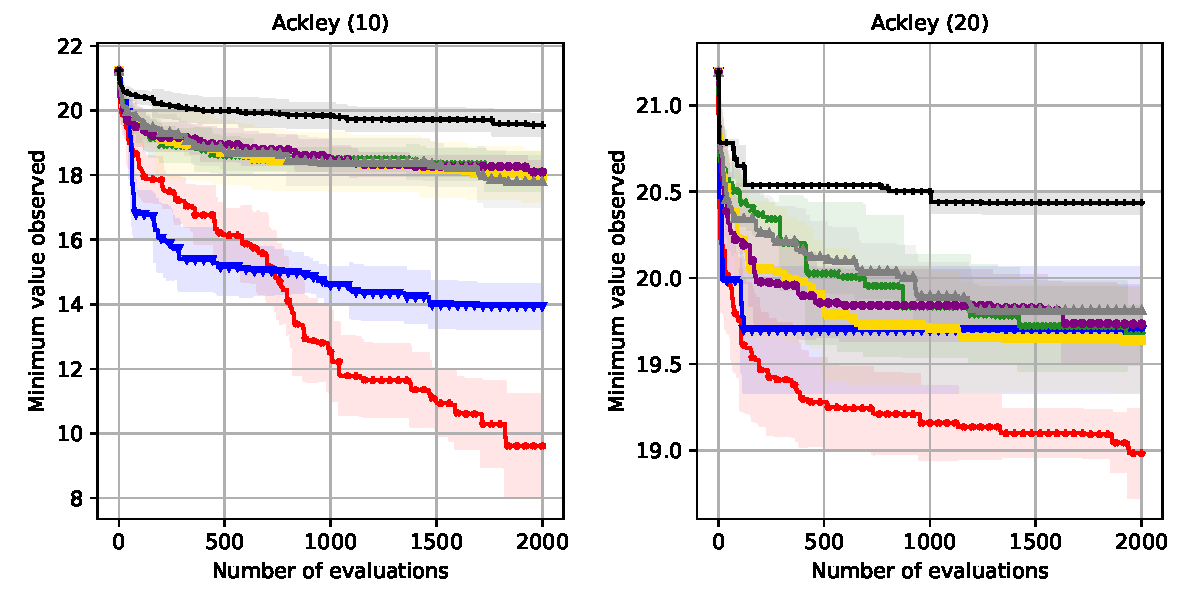
\includegraphics[width=\textwidth]{Figures/Neural-BO/A1.pdf}
    \end{subfigure}
    \begin{subfigure}[b]{\textwidth}
        \centering
        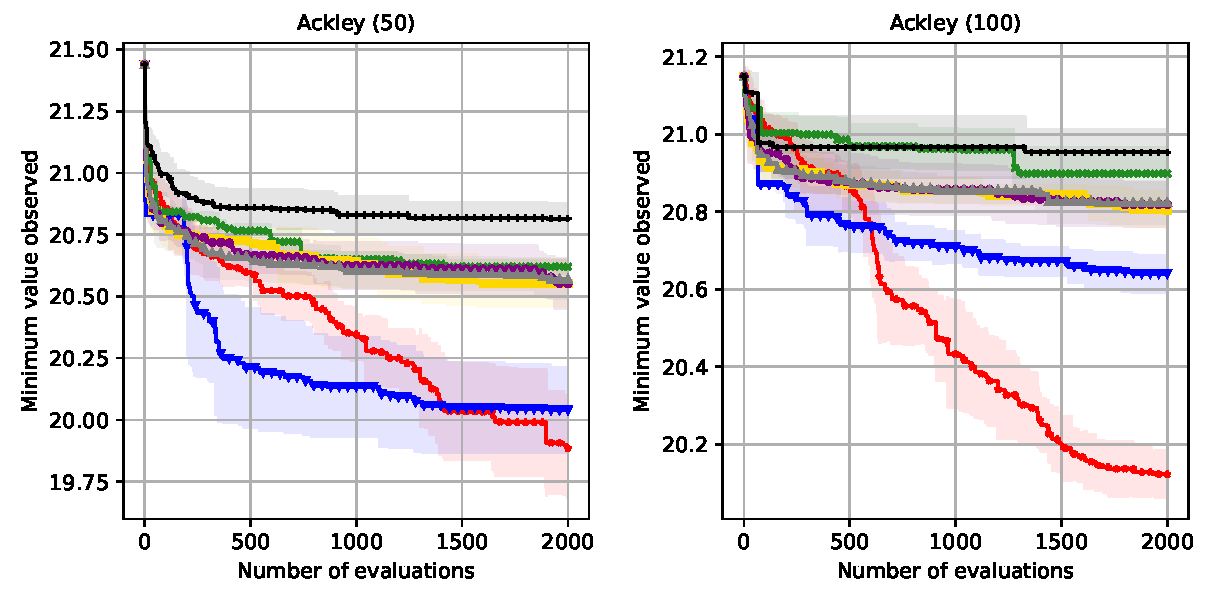
\includegraphics[width=\textwidth]{Figures/Neural-BO/A2.pdf}
    \end{subfigure}
    \begin{subfigure}[b]{\textwidth}
        \centering
        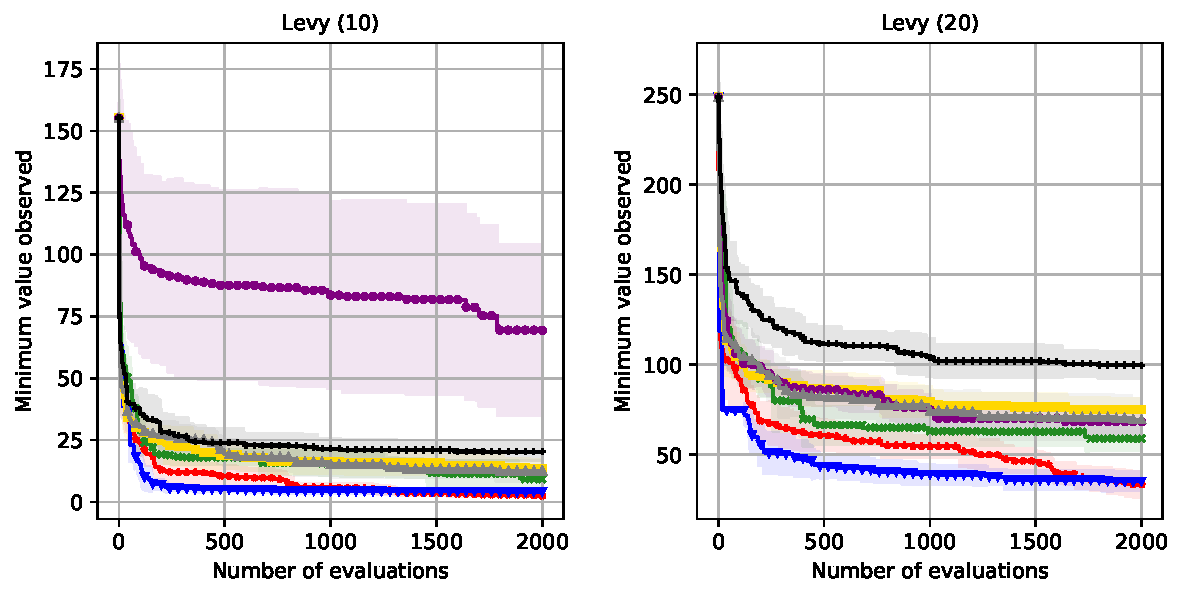
\includegraphics[width=\textwidth]{Figures/Neural-BO/L1.pdf}
    \end{subfigure}
    \label{fig:neural-bo_synthetic_1}
\end{figure}


\begin{figure}[]
    \centering
    \ContinuedFloat
    \begin{subfigure}[b]{\textwidth}
        \centering
        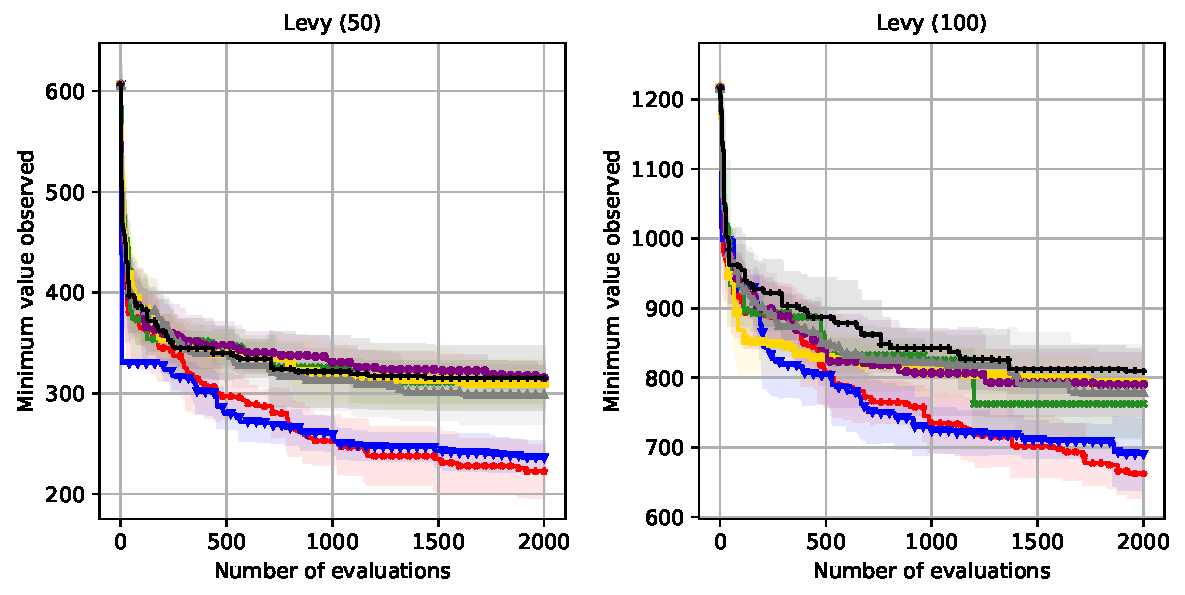
\includegraphics[width=\textwidth]{Figures/Neural-BO/L2.pdf}
    \end{subfigure}
    \begin{subfigure}[b]{\textwidth}
        \centering
        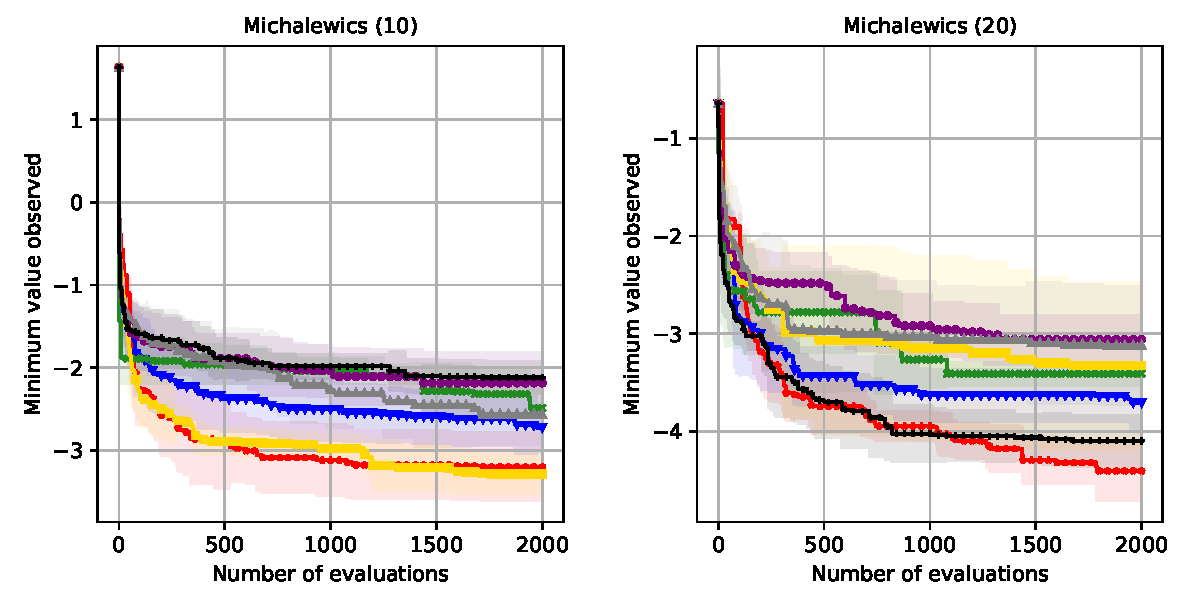
\includegraphics[width=\textwidth]{Figures/Neural-BO/M1.pdf}
    \end{subfigure}
    \begin{subfigure}[b]{\textwidth}
        \centering
        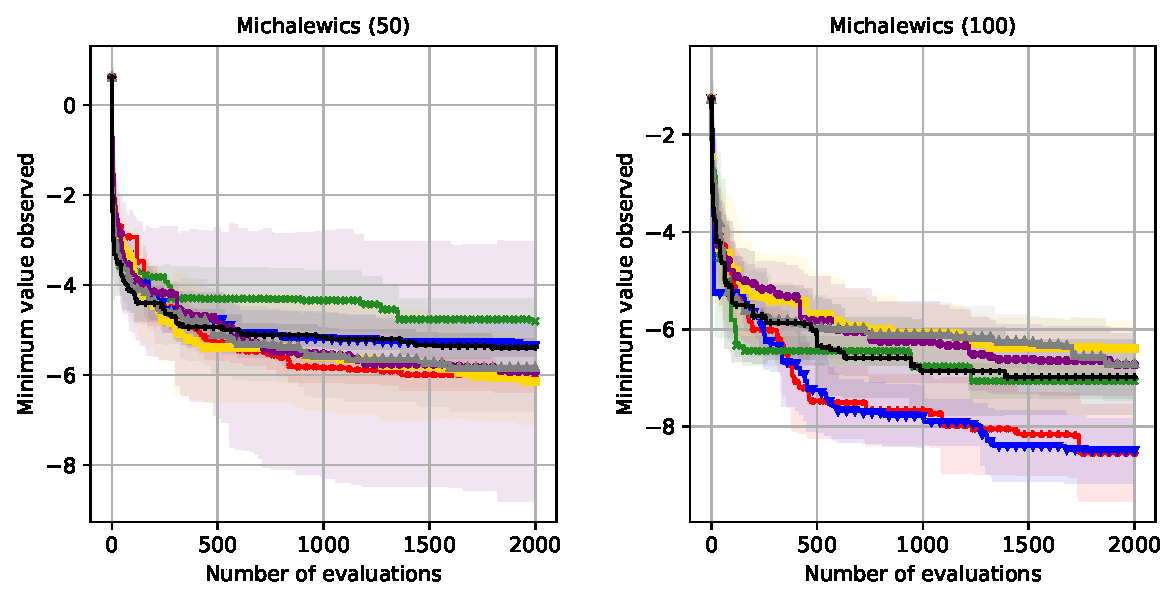
\includegraphics[width=\textwidth]{Figures/Neural-BO/M2.pdf}
    \end{subfigure}
    \begin{subfigure}[b]{0.8\textwidth}
        \centering
        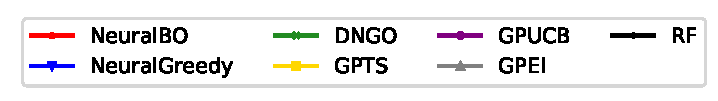
\includegraphics[width=\textwidth]{Figures/Neural-BO/baselines.pdf}
    \end{subfigure}
    \caption{The plots show the minimum true value observed after optimizing several synthetic functions over 2000 iterations of our proposed algorithm and 6 baselines. The dimension of each function is shown in the parenthesis.}
    \label{fig:neural-bo_synthetic}
\end{figure}




All reported experiments are averaged over 10 runs, each using a random initialization. All the methods start with the same set of initial points. As seen from Figure \ref{fig:neural-bo_synthetic}, Neural-BO is comparable to or better than all other baselines, including GP-based BO algorithms, both NN-based BO algorithms (DNGO and NeuralGreedy) and one algorithm using random forest. Moreover, our algorithm is also promising for high dimensions. 



In order to assess the statistical significance of whether our proposed method outperforms all baselines, we conducted a series of tests. First, a Kolmogorov-Smirnov (KS) test was performed to check if the sample sets for the hypothesis test follow a normal distribution. The null hypothesis assumes no difference between the observed and normal distribution. The p-values obtained from the KS test are presented in Table \ref{tab:ks_test}.  As all p-values exceeded 0.05, we failed to reject the null hypothesis, indicating that all data can be considered as normally distributed. Subsequently, one-sided t-tests were employed (as the variance is unknown), along with the Benjamini-Hochberg correction for multiple hypotheses testing, for each pair of (baseline, Neural-BO). These tests aimed to determine whether the baseline achieves a lower objective function value than our proposed method, Neural-BO. The alternative hypothesis $H_a: \mu_\text{baseline} > \mu_{\text{Neural-BO}}$ was tested against the null hypothesis $H_0: \mu_\text{baseline} \le \mu_{\text{Neural-BO}}$. Detailed test results are provided in Table \ref{tab:t-test}, where each cell contains two values: the first value represents the p-value obtained from the t-test, and the second value (T or F) indicates the outcome of the Benjamini-Hochberg correction where "T" indicates that the null hypothesis is rejected, whereas an "F" indicates that it is not rejected.







\begin{table}[]
\resizebox{\textwidth}{!}{
\begin{tabular}{|cc|c|c|c|c|c|c|c|}
\hline
\multicolumn{2}{|c|}{}                                                                                          & \textbf{\begin{tabular}[c]{@{}c@{}}Neural\\-BO\end{tabular}} & \textbf{\begin{tabular}[c]{@{}c@{}}Neural\\ Greedy\end{tabular}} & \textbf{\begin{tabular}[c]{@{}c@{}}GP\\-UCB\end{tabular}} & \textbf{\begin{tabular}[c]{@{}c@{}}GP\\-TS\end{tabular}} & \textbf{\begin{tabular}[c]{@{}c@{}}GP\\-EI\end{tabular}} & \textbf{DNGO} & \textbf{RF} \\ \hline
\multicolumn{1}{|c|}{\multirow{4}{*}{\textbf{Ackley}}}                                                  & D=10  & 0.85                                                         & 0.83                                                             & 0.95                                                      & 0.95                                                     & 0.45                                                     & 0.23          & 0.79        \\ \cline{2-9} 
\multicolumn{1}{|c|}{}                                                                                  & D=20  & 0.31                                                         & 0.46                                                             & 0.91                                                      & 0.90                                                     & 1.00                                                     & 1.00          & 0.93        \\ \cline{2-9} 
\multicolumn{1}{|c|}{}                                                                                  & D=50  & 0.95                                                         & 0.38                                                             & 0.81                                                      & 0.99                                                     & 0.52                                                     & 0.85          & 0.67        \\ \cline{2-9} 
\multicolumn{1}{|c|}{}                                                                                  & D=100 & 0.84                                                         & 0.77                                                             & 0.94                                                      & 0.82                                                     & 0.82                                                     & 0.38          & 0.97        \\ \hline
\multicolumn{1}{|c|}{\multirow{4}{*}{\textbf{Levy}}}                                                    & D=10  & 0.75                                                         & 0.45                                                             & 0.79                                                      & 0.72                                                     & 0.72                                                     & 0.58          & 0.63        \\ \cline{2-9} 
\multicolumn{1}{|c|}{}                                                                                  & D=20  & 0.84                                                         & 1.00                                                             & 1.00                                                      & 0.79                                                     & 0.79                                                     & 0.91          & 0.89        \\ \cline{2-9} 
\multicolumn{1}{|c|}{}                                                                                  & D=50  & 0.76                                                         & 0.34                                                             & 0.75                                                      & 0.75                                                     & 0.98                                                     & 0.77          & 0.37        \\ \cline{2-9} 
\multicolumn{1}{|c|}{}                                                                                  & D=100 & 0.76                                                         & 0.59                                                             & 0.87                                                      & 0.90                                                     & 0.99                                                     & 0.93          & 0.95        \\ \hline
\multicolumn{1}{|c|}{\multirow{4}{*}{\textbf{\begin{tabular}[c]{@{}c@{}}Micha-\\ lewics\end{tabular}}}} & D=10  & 0.54                                                         & 0.56                                                             & 0.95                                                      & 0.88                                                     & 0.83                                                     & 0.77          & 0.55        \\ \cline{2-9} 
\multicolumn{1}{|c|}{}                                                                                  & D=20  & 0.60                                                         & 0.99                                                             & 0.43                                                      & 0.33                                                     & 0.31                                                     & 0.56          & 0.85        \\ \cline{2-9} 
\multicolumn{1}{|c|}{}                                                                                  & D=50  & 0.90                                                         & 0.80                                                             & 0.64                                                      & 0.39                                                     & 0.68                                                     & 0.99          & 0.95        \\ \cline{2-9} 
\multicolumn{1}{|c|}{}                                                                                  & D=100 & 0.70                                                         & 0.58                                                             & 0.96                                                      & 0.57                                                     & 0.96                                                     & 0.93          & 0.52        \\ \hline
\end{tabular}
}
\caption{The p-values of KS-test "whether the data obtained from running our methods Neural-BO and all baselines are normally distributed".}
\label{tab:ks_test}
\end{table}



% \begin{table}[H]
% \begin{tabular}{|c||c|c|c|}\hline
% \backslashbox[0.\linewidth]{DIM}{Obj}
% &\makebox[0.22\linewidth]{Ackley}&\makebox[0.22\linewidth]{Levy}&\makebox[0.22\linewidth]{Michalewics}\\\hline
% 10&(-7.51, 5.95e-14)&(-4.4, 1.06e-05)&(0.574, 0.566)\\\hline
% 20&(-4.99, 5.95e-07)&(-0.6, 0.548)&(-2.32, 0.0203)\\\hline
% 50&(-1.77, 0.0465)&(-1.35, 0.177)&(0.216, 0.829)\\\hline
% 100&(-20.2, 4.35e-91)&(-1.36, 0.175)&(-0.126, 0.899)\\\hline
% \end{tabular}
% \caption{The z-scores and p-values of the z-test "whether our proposed Neural-BO achieves lower function value than that of the runner-up baseline" for the synthetic function optimizations in Figure \ref{fig:synthetic}.}
% \label{tab:pvalue}
% \end{table}
\begin{table}[]
\resizebox{\textwidth}{!}{
\begin{tabular}{|cc|l|l|l|l|l|l|}
\hline
\multicolumn{2}{|c|}{}                                                                                          & \multicolumn{1}{c|}{\textbf{\begin{tabular}[c]{@{}c@{}}Neural\\ Greedy\end{tabular}}} & \multicolumn{1}{c|}{\textbf{GPUCB}} & \multicolumn{1}{c|}{\textbf{GPTS}} & \multicolumn{1}{c|}{\textbf{GPEI}} & \multicolumn{1}{c|}{\textbf{DNGO}} & \multicolumn{1}{c|}{\textbf{RF}} \\ \hline
\multicolumn{1}{|c|}{\multirow{4}{*}{\textbf{Ackley}}}                                                  & D=10  & (2.98e-07,   T)                                                                       & (3.11e-12, T)                       & (1.64e-11, T)                      & (2.3e-11, T)                       & (6.15e-09, T)                      & (2.09e-13, T)                    \\ \cline{2-8} 
\multicolumn{1}{|c|}{}                                                                                  & D=20  & (6.39e-05, T)                                                                         & (1.61e-06, T)                       & (4.72e-05, T)                      & (4.19e-08, T)                      & (0.000111, T)                      & (1.29e-05, T)                    \\ \cline{2-8} 
\multicolumn{1}{|c|}{}                                                                                  & D=50  & (0.0467, T)                                                                           & (2.23e-08, T)                       & (1.89e-08, T)                      & (8.5e-09, T)                       & (1.86e-08, T)                      & (2.11e-10, T)                    \\ \cline{2-8} 
\multicolumn{1}{|c|}{}                                                                                  & D=100 & (3.92e-14, T)                                                                         & (7.98e-16, T)                       & (2.43e-16, T)                      & (4.7e-16, T)                       & (6.44e-16, T)                      & (5.78e-17, T)                    \\ \hline
\multicolumn{1}{|c|}{\multirow{4}{*}{\textbf{Levy}}}                                                    & D=10  & (0.000171, T)                                                                         & (7.98e-06, T)                        & (8.81e-09, T)                      & (6.6e-07, T)                       & (1.68e-05, T)                      & (1.62e-11, T)                    \\ \cline{2-8} 
\multicolumn{1}{|c|}{}                                                                                  & D=20  & (0.278, F)                                                                            & (3.28e-09, T)                       & (4.32e-11, T)                      & (1.8e-07, T)                       & (4.75e-05, T)                      & (8.01e-14, T)                    \\ \cline{2-8} 
\multicolumn{1}{|c|}{}                                                                                  & D=50  & (0.0971, F)                                                                           & (5.37e-09, T)                       & (2.72e-07, T)                      & (6.47e-06, T)                      & (0.000188, T)                      & (1.99e-06, T)                    \\ \cline{2-8} 
\multicolumn{1}{|c|}{}                                                                                  & D=100 & (0.096, F)                                                                            & (1.09e-06, T)                       & (4.85e-08, T)                      & (9.87e-05, T)                      & (0.00456, T)                       & (5.57e-07, T)                    \\ \hline
\multicolumn{1}{|c|}{\multirow{4}{*}{\textbf{\begin{tabular}[c]{@{}c@{}}Micha-\\ lewics\end{tabular}}}} & D=10  & (5.9e-06, T)                                                                          & (7.79e-08, T)                       & (0.472, F)                         & (1.68e-05, T)                      & (7.49e-06, T)                      & (1.87e-11, T)                    \\ \cline{2-8} 
\multicolumn{1}{|c|}{}                                                                                  & D=20  & (2.63e-05, T)                                                                         & (3e-09, T)                          & (0.00108, T)                       & (1.02e-05, T)                      & (0.000163, T)                      & (0.0161, T)                      \\ \cline{2-8} 
\multicolumn{1}{|c|}{}                                                                                  & D=50  & (0.000344, T)                                                                         & (3.47e-06, T)                       & (0.315, F)                         & (0.101, F)                         & (0.000871, T)                      & (0.000132, T)                    \\ \cline{2-8} 
\multicolumn{1}{|c|}{}                                                                                  & D=100 & (0.45, F)                                                                             & (8.2e-05, T)                        & (8.49e-06, T)                      & (0.000126, T)                      & (0.0404, T)                        & (0.00579, T)                     \\ \hline
\end{tabular}
}
\caption{One-sided t-tests were employed to assess whether the baseline achieves a lower function value compared to our proposed method, Neural-BO.  The null hypothesis $H_0: \mu_\text{baseline} \le \mu_{\text{Neural-BO}}$ and the alternative hypothesis:  $H_a: \mu_\text{baseline} > \mu_{\text{Neural-BO}}$. The p-value corresponding to each test is provided as the first value in each cell. Moreover, to account for multiple hypotheses testing, the Benjamini-Hochberg correction was applied and is reported as the second value in each cell. In the outcome, a "T" indicates that the null hypothesis is rejected, whereas an "F" signifies that it is not rejected.}
\label{tab:t-test}
\end{table}


Next, we used the COmparing Continuous Optimizers (COCO) framework\footnote{ \url{https://github.com/numbbo/coco}} to compare the performance of our method with baseline methods. COCO is a widely used benchmarking platform for continuous optimization algorithms, providing researchers with a standardized set of test functions to evaluate different optimization methods. The framework includes a collection of test functions that are designed to be challenging to optimize and exhibit various properties, such as multimodality, ill-conditioning, or weak global structure. To evaluate our algorithms, we used the BBOB test functions, which consist of 24 noiseless, single-objective, and scalable functions. The quality indicator needs to reach or exceed a predefined target value  $t$  for COCO to consider a single run over a problem successful. The performance of different optimizers is measured by the \textit{Fraction of function, target pairs}, which indicates the ratio of problems solved at optimization step $T$. For more details on how COCO measures the performance of different optimizers, please refer to \citet{hansen2021coco}. We set the number of evaluations for our optimizers to be 20 times the dimension of the problem. 

\begin{figure}[]
\begin{subfigure}{.5\textwidth}
  \centering
  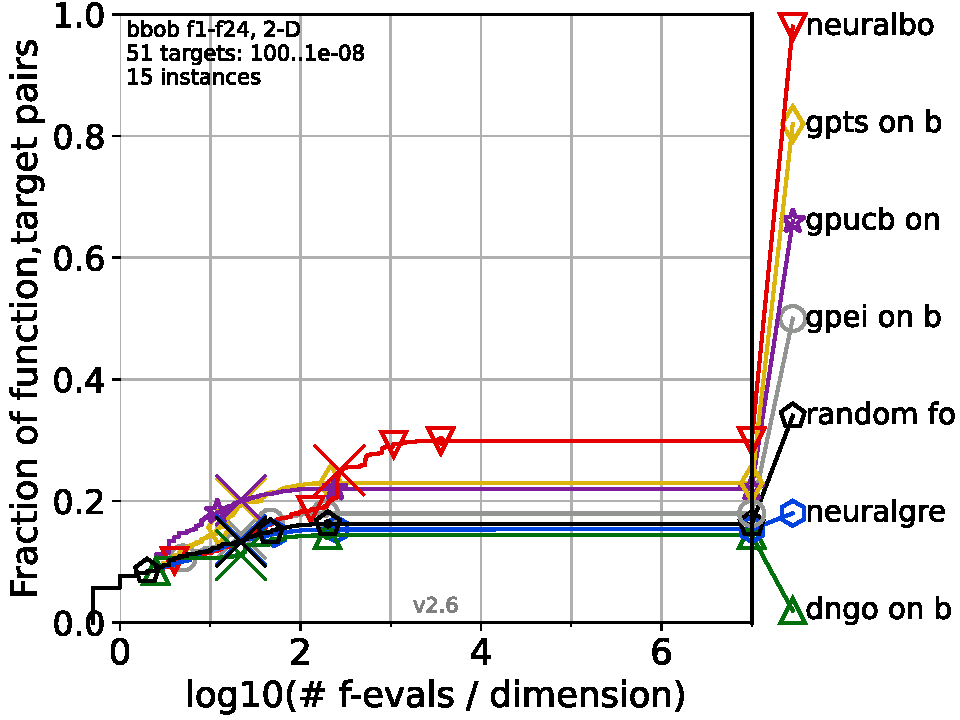
\includegraphics[width=\linewidth]{Figures/Neural-BO/Neural-BO_pprldmany_02D_noiselessall.pdf}
  \caption{2D}
  \label{fig:coco_2d}
\end{subfigure}%
\begin{subfigure}{.5\textwidth}
  \centering
  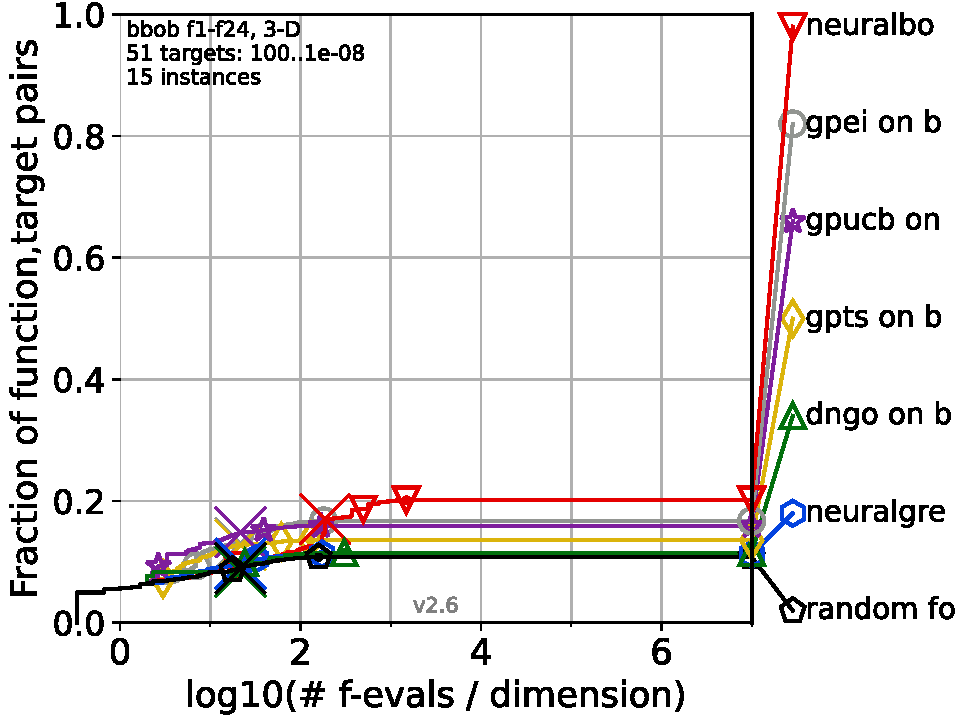
\includegraphics[width=\linewidth]{Figures/Neural-BO/Neural-BO_pprldmany_03D_noiselessall.pdf}
  \caption{3D}
  \label{fig:coco_3d}
\end{subfigure}
\begin{subfigure}{.5\textwidth}
  \centering
  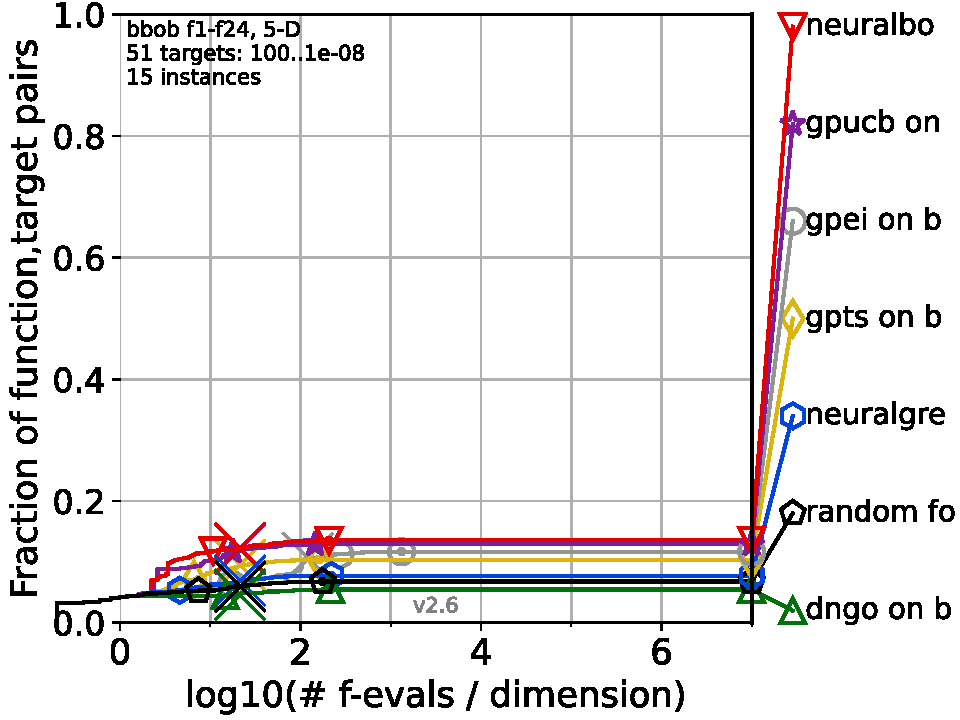
\includegraphics[width=\linewidth]{Figures/Neural-BO/Neural-BO_pprldmany_05D_noiselessall.pdf}
  \caption{5D}
  \label{fig:coco_5d}
\end{subfigure}%
\begin{subfigure}{.5\textwidth}
  \centering
  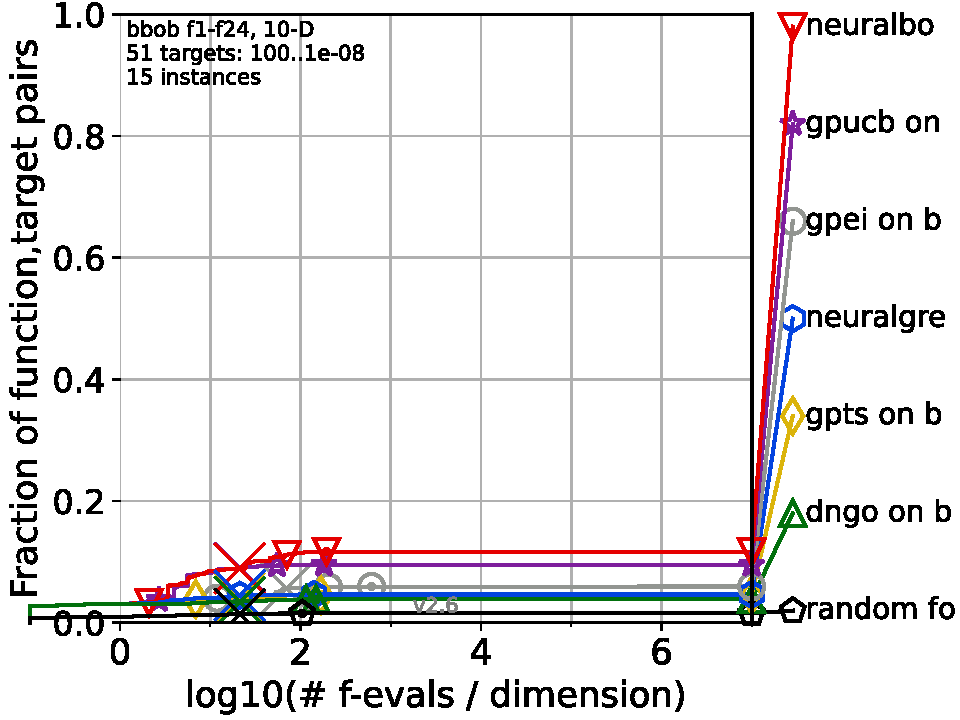
\includegraphics[width=\linewidth]{Figures/Neural-BO/Neural-BO_pprldmany_10D_noiselessall.pdf}
  \caption{10D}
  \label{fig:coco_10d}
\end{subfigure}
\caption{The results of benchmarking our Neural-BO and the baselines with COCO framework on 24 BBOB noiseless objective functions with four different dimensions \{2,3,5,10\}.}
\label{fig:coco}
\end{figure}

In Figure \ref{fig:coco}, we present the results of our experiment using the COCO benchmarking framework to evaluate all methods. The benchmarking comprised 24 noiseless functions with 15 instances, where each instance represented a unique condition of the function, such as the location of the optimum. Our method was found to outperform other baselines when assessed using the well-designed and publicly available COCO framework. 


\subsection{Real-world Applications}
\subsubsection{Designing Sensitive Samples for Detection of Model Tampering}
\label{section:neural-bo_sensitive_samples}
\begin{figure}[H]
    \centering
    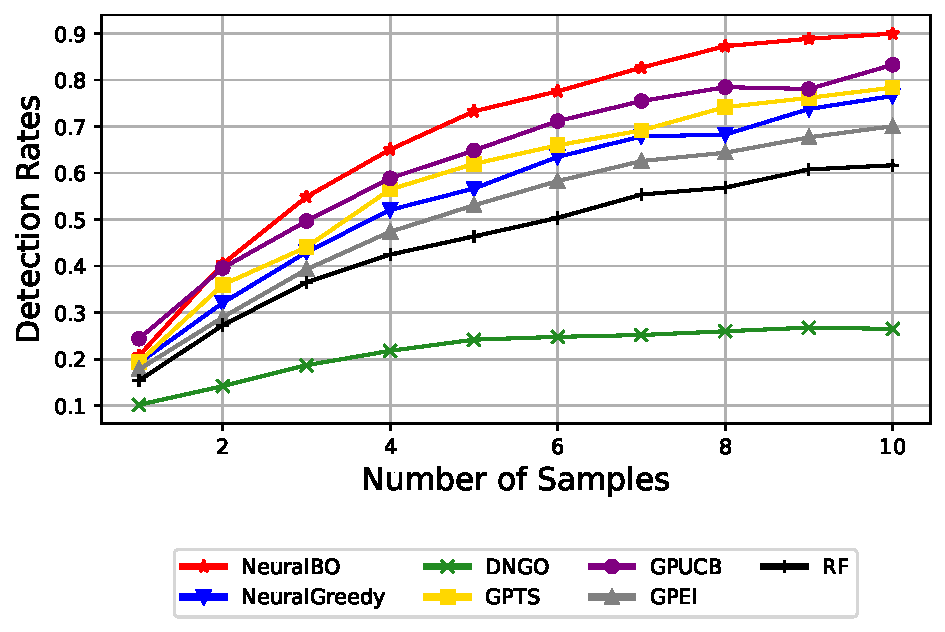
\includegraphics[width=\textwidth]{Figures/Neural-BO/Neural-BO_sensitive_sample_detection_rate.pdf}
    \caption{The plot shows the \textbf{detection rates} corresponding to the number of samples on the MNIST dataset. The larger the number of sensitive samples, the higher the detection rate. As shown in the figure, Neural-BO can generate sensitive samples that achieve nearly 90\% of the detection rate with at least 8 samples.}
    \label{fig:neural-bo_sensitive_sample}
\end{figure}

We consider an attack scenario where a company offering Machine Learning as a service (MLaaS) hosts its model on a cloud. However, an adversary with backdoor access may tamper with the model to change its weight. This requires the detection of model tampering. To deal with this problem, \citet{he2018verideep} suggests generating a set of test vectors named \emph{Sensitive-Samples} $\{v_i\}_{i=1}^n$, whose outputs predicted by the compromised model will be different from the outputs predicted by the original model. As formalized in \citet{he2018verideep}, suppose we suspect a pre-trained model $f_\theta(x)$ of having been modified by an attacker after it was sent to the cloud service provider. Finding sensitive samples for verifying the model's integrity is equivalent to optimizing task: $v = \argmax_x \norm{\frac{\partial f_\theta(x)}{\partial \theta}}_F$, where $\norm{\cdot}_F$ is the Frobenius norm of a matrix. A \emph{successful detection} is defined as ``given $N_S$ sensitive samples, there is at least one sample, whose top-1 label predicted by the compromised model is different from the top-1 label predicted by the correct model''. Clearly, optimizing this expensive function requires a BO algorithm to be able to work with high-dimensional structured images, unlike usual inputs that take values in hyper-rectangles.

We used a handwritten digit classification model (pre-trained on MNIST data) as the original model and tampered it by randomly adding noise to each weight of this model. We repeat this procedure 1000 times to generate 1000 different tampered models. The top-1 accuracy of the MNIST original model is $93\%$ and is reduced to $87.73\% \pm 0.08\%$ after modifications.   

To reduce the computations, we reduce the dimension of images from $28 \times 28$ to $7 \times 7$ and do the optimization process in 49-dimensional space. After finding the optimal points, we recover these points to the original dimension by applying an upscale operator to get sensitive samples. We compare our method with all other baselines by the average detection rate with respect to the number of sensitive samples. From Figure \ref{fig:sensitive_sample}, it can be seen that our method can generate  samples with better detection ability than other baselines. This demonstrates the ability of  our method to deal with complex structured data such as images. 

\subsubsection{Unknown target document retrieval}
\begin{figure}[H]
    \centering
    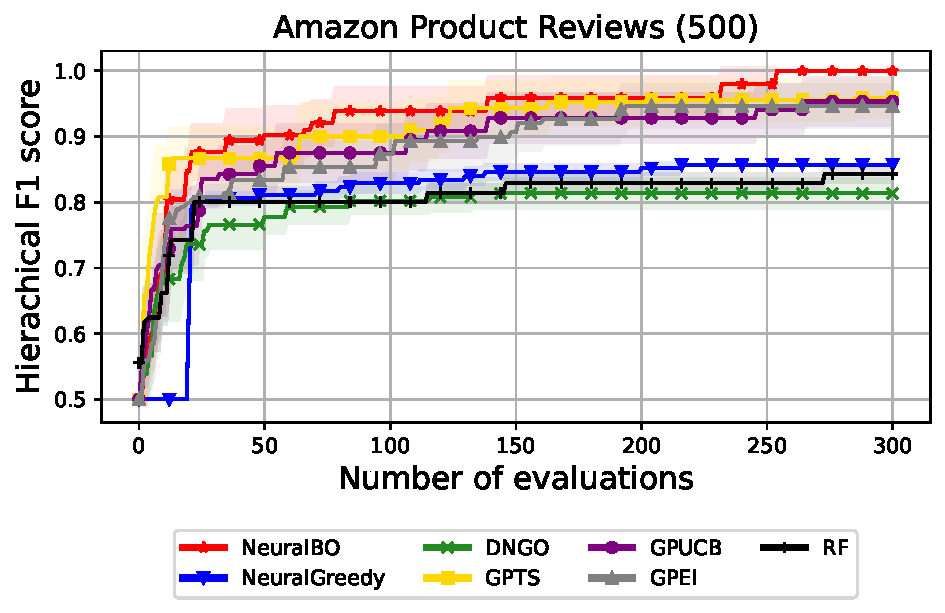
\includegraphics[width=\textwidth]{Figures/Neural-BO/Neural-BO_AmazonReview_dim_500_round_300.pdf}
    \caption{We search for the most related document for a specified target document in \textbf{Amazon product reviews} dataset and report the maximum \textbf{hierachical F1 score} found by all baselines. All methods show similar behaviour and Neural-BO performs comparably and much better than GP-based baselines.}
    \label{fig:text}
\end{figure}
Next, we evaluate our proposed method on a retrieval problem where our goal is to retrieve a document from a corpus that matches user's preference. The optimization algorithm works as follows: it retrieves a document, receives user's feedback score and then updates its belief and attempts again until it reaches a high score, or its budget is depleted. The objective target function is defined as the user’s evaluation of each document, which usually has a complex structure. It is clear that evaluations are expensive since the user must read each suggestion. Searching for the most relevant document is considered as finding document $d$ in the dataset $S_{text}$ that maximizes the match to the target document $d_t$: $d = \argmax_{d \in S_{text}} \textup{Match}(d, d_t)$, where $\textup{Match}(d, d_t)$ is a matching score between documents $d$ and $d_t$. We represent each document by a word frequency vector $x_{n} = (x_{n1}, \cdots, x_{nJ})$, where $x_{nj}$ is the number of occurrences of the $j$-th vocabulary term in the $n$-th document, and $J$ is the vocabulary size.  

Our experiment uses Amazon product reviews 
dataset\footnote{\url{https://www.kaggle.com/datasets/kashnitsky/hierarchical-text-classification}}, which are taken from users' product reviews from Amazon's online selling platform. This dataset has hierarchical categories, where the category classes are sorted from general to detail. The dataset is structured as: 6 classes in ``level 1'', 64 classes in ``level 2'' and 464 classes in ``level 3''. The number of users' reviews was originally 40K, which was reduced to 37738 after ignoring reviews with ``unknown'' category. We choose the size of vocabulary to be 500 and use the hierarchical F1-score introduced in  \citet{kiritchenko2005functional} as a scoring metric for the target and retrieved documents. We report the mean and standard deviation of hierarchical F1-score between target and retrieved documents over ten runs for all methods in Figure \ref{fig:text}. Figures \ref{fig:text} indicate that our method shows a better performance for the Amazon product review dataset in comparison with other approaches. 

\subsubsection{Optimizing control parameters for robot pushing} 
\begin{figure}[H]
    \centering
    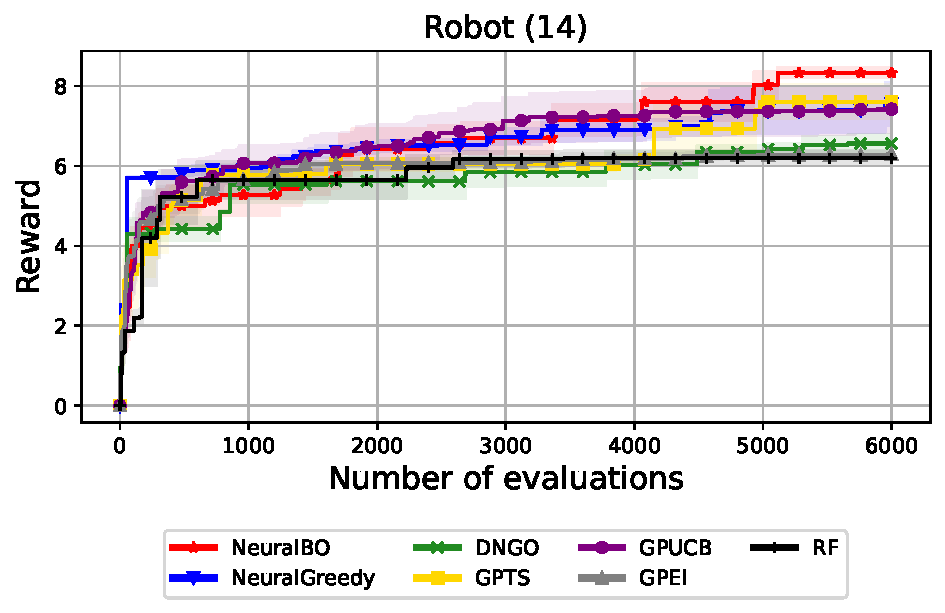
\includegraphics[width=\textwidth]{Figures/Neural-BO/Neural-BO_Robot_dim_14_round_6000.pdf}
    \vspace{-3mm}
    \caption{
    Optimization results for control parameters of 14D robot pushing problem. The X-axis shows iterations, and the y-axis shows the median of the best reward obtained.}
    \label{fig:robot_14D}
\end{figure}

Finally, we evaluate our method on tuning control parameters for the robot pushing problem considered in \citet{wang2017max}. We run each method for a total of 6000 evaluations and repeat ten times to take average optimization results. Neural-BO and all other methods are initialized with 15 points. Figure \ref{fig:robot_14D} summarizes the median of the best rewards achieved by all methods. It can be seen that Neural-BO achieves the highest reward after 5K optimization steps. 

\section{Conclusion}
We proposed a new algorithm for \acl{bo} using \aclp{dnn}. A key advantage of our algorithm is that it is computationally efficient and performs better than traditional \acl{gp} based methods, especially for complex structured design problems. We provided rigorous theoretical analysis for our proposed algorithm and showed that its cumulative regret converges with a sublinear regret bound. Using both synthetic benchmark optimization functions and a few real-world optimization tasks, we showed the effectiveness of our proposed algorithm. 
\chapter{Black-box Optimization with Unknown Constraints via Overparameterized Deep Neural Networks} % Main chapter title
\label{chap:neural-cbo} % For referencing the chapter elsewhere, use \ref{chap:background}

\acl{bo} with \textit{unknown constraints} (CBO) adjusts the acquisition function to find solutions that satisfy constraints while optimizing the objective function. A well-known method, Expected Improvement with Constraints (cEI), incorporates feasibility into the optimization process, focusing on regions likely to contain feasible solutions.

Alternative approaches, such as Predictive Entropy Search with Constraints (PESC) \citep{hernandez2015predictive}, Min-Value Entropy Search \citep{takeno2022sequential}, Augmented Lagrangian Bayesian Optimization (ALBO) \citep{gramacy2016modeling}, and Bayesian Optimization with Unknown Constraints using the Alternating Direction Method of Multipliers (ADMMBO) \citep{ariafar2019admmbo}, use various techniques, from information-theoretic methods to numerical optimization strategies, as discussed in Section \ref{section:bo_unknown_constraints}. However, these methods rely on \acp{gp} as surrogate models, which suffer from poor computational scalability. The cubic complexity of kernel matrix inversion becomes impractical as the number of constraints increases.

In contrast, \acp{dnn} provide a scalable alternative. They perform exceptionally well in feature extraction and maintain linear complexity as the dataset size grows. While \acp{dnn} have been successful in unconstrained black-box optimization \citep{snoek2015scalable} and contextual bandits in discrete search spaces \citep{zhou2020neural,zhang2021neural}, their application to constrained black-box optimization with theoretical guarantees \emph{remains largely unexplored}. This \emph{gap} motivates the development of neural network-based methods for CBO.

This chapter inherits a similar motivation as in Chapter \ref{chap:neural-bo} to apply for \ac{bo} with unknown, expensive constraints setting. We provided Neural-CBO, a method to alternate canonical \ac{gp} by \ac{dnn} as the surrogate model to model both objective function and constraints in CBO. \textbf{The contributions of this chapter} are highlighted as follows:

\begin{itemize}
    \item We propose a \ac{dnn}-based black-box optimization algorithm with unknown constraints (Neural-CBO), where both the objective function and constraints are modeled using deep neural networks. We use \ac{ei} as the acquisition function to find the next samples in a feasible region which is determined using \acf{lcb} satisfaction conditions to all constraints. Using \ac{lcb}-based conditions ensure that the feasible regions of these constraints are covered by the regions suggested by these conditions (with our problem setting), while leaving spaces for constraint explorations, particularly when feasible regions are much smaller than the search space.
 

    \item We provide a theoretical analysis of our proposed Neural-CBO algorithm based on recent advances in \ac{ntk} theory. Under certain regularity assumptions, we show that cumulative regret as well as cumulative constraint violation has an upper bound of the form $\mathcal{O}(\gamma_T\sqrt{T})$, where $\gamma_T$ is the maximum information gain. This result is comparable to previous \ac{gp}-based methods. It is worth noting that, our \ac{dnn} models only required the network width as $m=\Omega(T)$  for the convergence. 
    \item We conduct benchmarking experiments on synthetic and real-world tasks to prove our algorithm's effectiveness empirically. The numerical results indicate that our algorithm achieves competitive performance with well-known approaches.
    \end{itemize}
\section{Problem Setting}
In this chapter, we tackle the problem of black-box optimization, where the search space is subject to constraints imposed by other unknown black-box functions. These constraints arise from \emph{real-valued} feedback $c_i(\mathbf{x})$, and the constraint condition $c_i(\mathbf{x})$ is satisfied if and only if $c_i(\mathbf{x}) \leq 0$.  
Formally, this problem is defined as follows:
\begin{equation*}
    \begin{split}
        & \underset{\mathbf{x} \in \mathcal{D}}{\min} f(\mathbf{x}),  \text{ subject to }  c_i (\mathbf{x})  \leq 0, \text{ for all } i = 1, \dots, K,
    \end{split}
\end{equation*}  
where $\mathcal{D} \subset \mathbb{R}^d$ is a bounded domain, and $f$ and $\{c_i\}_{i=1}^K \colon \mathbb{R}^d \rightarrow \mathbb{R}$ are unknown functions that can be evaluated at specific points. We consider this problem in a \textbf{coupled} setting, where both the objective function and constraints are evaluated simultaneously.


\section{Proposed Neural-CBO Method}
\label{section:neural-cbo}
Here, we first introduce the general \acp{dnn} architecture used to model the objective function and the constraints, followed by basis theoretical properties accompanying of these networks. Then, the Neural-CBO algorithm is introduced. 

\subsection{The \acl{dnn} for an Arbitrary Function $f_a$}
\label{section:neural-cbo_arbitrary_nn}
Given a black-box, expensive function $f_a$, we use a fully connected neural network, denoted as $a(\mathbf{x}; \mathbf{W})$, to model $f_a$:
\begin{equation}
\label{eqn:fcn}
    a(\mathbf{x}; \mathbf{W}) = \frac{\mathbf{q}^\top}{\sqrt{m}} \mathbf{D}^{(L)}(\mathbf{x}) \mathbf{W}^{(L)} \dots \frac{1}{\sqrt{m}} \mathbf{D}^{(1)}(\mathbf{x}) \mathbf{W}^{(1)} \mathbf{x}, 
\end{equation}
where $\mathbf{q} \in \mathbb{R}^m$ is the last layer weight, $\mathbf{W}^{(1)} \in \mathbb{R}^{m \times d}$, $\mathbf{W}^{(l)} \in \mathbb{R}^{m \times m}$ for $2 \leq l \leq L$ is the weight of the $l$-th hidden layer. The matrix $\mathbf{D}^{(l)}(\mathbf{x})$ is associated with the ReLU activation function and is defined as:
\begin{equation*}
    \mathbf{D}^{(l)}(\mathbf{x}) = \text{diag}\{\mathbf{1}_{ \{ \langle w_i^{(l)}, \mathbf{h}^{(l-1)}(\mathbf{x})  \rangle \ge 0 \} } \} \in \mathbb{R}^{m \times m},
\end{equation*}
with $m$ as the number of neurons in the hidden layer $l$, and $\mathbf{h}^{(l)}(\mathbf{x})$ is the output of the $l$-th layer given by 
\begin{equation*}
    \mathbf{h}^{(l)}(\mathbf{x}) = \frac{1}{\sqrt{m}} \mathbf{D}^{(l)}(\mathbf{x}) \mathbf{W}^{(l)} \dots \frac{1}{\sqrt{m}} \mathbf{D}^{(1)}(\mathbf{x}) \mathbf{W}^{(1)} \mathbf{x},
\end{equation*}
with $\mathbf{h}^{(0)}(\mathbf{x}) = \mathbf{x}$. 

At time $t=0$, each weight matrix $\mathbf{W}^{(l)},  2 \le l \le L$ is initialized as $\begin{bmatrix}
\boldsymbol{\Psi} & \mathbf{0}  \\
\mathbf{0} & \boldsymbol{\Psi}
\end{bmatrix}
$, where $\boldsymbol{\Psi}$ is a Gaussian random matrix with independent and identically distributed (i.i.d.) standard normal entries. Additionally, the outer weights $\mathbf{q} = (\hat{\mathbf{q}}, -\hat{\mathbf{q}})^\top$  are set as random variables, and each entry of $\mathbf{b}$ is set with an equal probability of being either $-1$ or $1$, and remain fixed throughout the training process. This initialization method is commonly employed in the literature, as seen in works like \citet{du2018gradient, arora2019fine}, and it
can be verified that, with this initialization scheme, $a(\mathbf{x}; \mathbf{W}_0) = 0$, for all input $\mathbf{x}$. 

The neural network is trained by running the stochastic gradient descent on the streaming data in \textit{one pass}. In particular, given the initialization $\{\mathbf{W}_0^{(l)} \}_{l=1}^L$ and last layer weight $\mathbf{q}$, the $l$-th layer weight matrix at the $t$-th iteration is updated by minimizing the $L_2$ loss as:
\begin{equation}
    \label{eqn:train_NN}
    \mathbf{W}_{t+1}^{(l)} = \mathbf{W}_{t}^{(l)} + \alpha_t (y_t - a(\mathbf{x}_t; \mathbf{W}_t)) \frac{\partial a(\mathbf{x}_t; \mathbf{W}_t)}{\partial \mathbf{W}^{(l)}},
\end{equation}
where $\alpha_t$ is the step size, and $\{\mathbf{x}_t, y_t\}$ is the observation at the $t$-th optimization iteration. 


% $\phi\colon \mathbb{R} \rightarrow \mathbb{R}$ is the ReLU activation function, and the weights $\mathbf{W}_1 \in \mathbb{R}^{m \times d}$, $\mathbf{W}_i \in \mathbb{R}^{m \times m}$ for $2 \leq i \leq L-1$, and $\mathbf{W}_L \in \mathbb{R}^{1 \times m}$ are the neural network parameters $\mathbf{W} \in \mathbb{R}^p$, with $p = md + m^2(L-2) + m$. The input dimension is $d$, where $\mathbf{x} \in \mathcal{D} \subset \mathbb{R}^d$, and the weights are initialized from a standard normal distribution $\mathcal{N}(0,1)$.

To estimate the uncertainty of the function $f_a$ modeled by $a(\mathbf{x}; \mathbf{W})$, we adopt the variance formula from recent advances in neural contextual bandits research ~\citep{zhou2020neural, kassraie2022neural}:
\begin{equation}
    \label{Eqn:neural_cbo_variance_formula}
    \sigma_{a,t}(\mathbf{x}) = \sqrt{\mathbf{g}_{a}(\mathbf{x}; \mathbf{W}_0)^\top \mathbf{U}_{a, t-1}^{-1} \mathbf{g}_{a}(\mathbf{x}; \mathbf{W}_0)},
\end{equation}
where

\begin{equation}
\label{eqn:ntk_cov}
\begin{aligned}
    \mathbf{g}_{a}(\mathbf{x}; \mathbf{W}) &= \nabla_{\mathbf{W}}a(\mathbf{x}; \mathbf{W}), \text{ and}\\
     \mathbf{U}_{a, t} &= \mathbf{U}_{a, t-1} + \mathbf{g}_{a}(\mathbf{x}_t; \mathbf{W}_0) \mathbf{g}_{a}(\mathbf{x}_t; \mathbf{W}_0)^\top,
\end{aligned}
\end{equation}

We again inherit the concept of \acf{ntk} introduced in Section \ref{section:NTK} for our theoretical analysis. We briefly remind this concept through the following definition: 
\begin{definition}
    \label{def:neural-cbo_ntk}
    Given the $L$-layer neural network $a(\mathbf{x}; \mathbf{W})$ with input $\mathbf{x}$ and parameter $\mathbf{W}$ as defined in Eqn. \ref{eqn:fcn}, a \ac{ntk} matrix $\mathbf{H}_t$ for a sequence of weights {$\mathbf{W}_t$} can be defined as:
    \begin{equation*}
        \mathbf{H}_t [i, j] \coloneqq \left \langle \frac{\partial a(\mathbf{x}_i; \mathbf{W}_t)}{\partial \mathbf{W}},  \frac{\partial a(\mathbf{x}_j; \mathbf{W}_t)}{\partial \mathbf{W}}\right \rangle = \sum_{l=1}^L \mathbf{H}^{(l)}_t[i, j],
    \end{equation*}
    where $\mathbf{H}^{(l)}_t [i, j] \coloneqq \left \langle \frac{\partial a(\mathbf{x}_i; \mathbf{W}_t)}{\partial \mathbf{W}^{(l)}},  \frac{\partial a(\mathbf{x}_j; \mathbf{W}_t)}{\partial \mathbf{W}^{(l)}}\right \rangle$ is the NTK from the $l$-th hidden layer, for all $1 \le i, j \le T$.
\end{definition}


Next, we present the common and well-established assumptions. The following assumption indicates the smoothness property of the unknown function $f_a$.
\begin{assumption}
\label{assumption:rkhs}
We assume that $f_a \in \mathcal{H}_{k_a}(\mathcal{D})$, where $\mathcal{H}_{k_a}(\mathcal{D})$ is the Reproducing Kernel Hilbert Space (RKHS) associated with a real-valued function $f_a$ defined on the domain $\mathcal{D}$. This space is induced by the Neural Tangent Kernel $k_a$, which arises from a neural network $a(\mathbf{x}; \mathbf{W})$. In particular, the RKHS $\mathcal{H}_{k_a}$ induces an inner product $\langle \cdot, \cdot \rangle_{\mathcal{H}_{k_a}} $ with the reproducing property: for all $f_a \in \mathcal{H}_{k_a}(\mathcal{D})$, we have 
$f_a(\mathbf{x}) = \langle f_a, k_a(\cdot, \mathbf{x}) \rangle_{\mathcal{H}_{k_a}}$. 
The induced norm is bounded and 
serves as a measure of the smoothness of $f_a$ w.r.t the kernel function $k_a$: $\norm{f_a}_{\mathcal{H}_{k_a}} = \sqrt{\langle f_a, f_a \rangle_{\mathcal{H}_{k_a}}} \leq B_a$. 
\end{assumption}


To ensure that the noise arising from querying unknown function $f_a$ remains bounded and manageable, we impose the following assumption:
\begin{assumption}
\label{assumption:subgaussian_noise}
    We assume the noises $\{\zeta_{ t}\}_{t=1}^T$ where $\zeta_t = o_t - f_a(\mathbf{x}_t)$  are conditionally sub-Gaussian with parameter $R_{a} > 0$, where $\{\zeta_t\}_{t=1}^T$ is assumed to capture the noises induced by querying the black-box, expensive function $f_a(\cdot)$.
 \begin{equation*}
         \forall t \ge 0 , \; \forall \lambda_a \in \mathbb{R}, \;  \mathbb{E}[e^{\lambda_a\zeta_t} \rvert \mathcal{F}_{a,t-1}] \le \exp(\frac{\lambda_a^2 R_a^2}{2}),
 \end{equation*}
 where $\mathcal{F}_{a, t-1}$ are the $\sigma$-algebra generated by the random variables $\{\mathbf{x}_i, \zeta_i\} 
^{t-1}_{i=1} \cup \{\mathbf{x}_t\}$.
\end{assumption}

To manage the approximation error, several technical lemmas impose the following condition on the width of the neural network introduced in Eqn. \ref{eqn:fcn}.
\begin{condition}
    \label{condition:network_width}
    Throughout the section, the width of each hidden layer m satisfies is assumed to satisfy:
    \begin{align}
        m \ge d^9 \exp (\Omega(\nu LC^L\log T)), 
    \end{align}
for some absolute constant $C$. Besides, the step size $\alpha_t \le \frac{\nu}{t+1}$, where $\nu$ is a parameter and independent of dimension $d$ and width $m$.
\end{condition}


Before going to our \textbf{main algorithm}, we provide the confidence bound, the fundamental component in almost all \ac{bo} algorithms to guide algorithm design and ensure theoretical guarantee. The lemma demonstrates that by following the network width condition stated in Condition \ref{condition:network_width},  the prediction of the trained neural network $a(\cdot;\mathbf{W}_{t-1})$ is concentrated at the actual value of the function $f_a(\cdot)$. 
\begin{restatable}{lemma}{ConfidenceBound}

\label{lemma:neural-cbo_confidence_bound}
Let Assumptions \ref{assumption:rkhs} and \ref{assumption:subgaussian_noise} hold. Using neural network $a(\mathbf{x}; \mathbf{W})$ satisfied Condition \ref{condition:network_width} to model an arbitrary function $f_a$. Setting the step size at training step $t$ as $\alpha_t \le \frac{\nu}{(T+1)^2}$, then for any $\delta \in (0,1)$,  with probability at least $1 - \delta \exp (\Omega(C^{-L} m^{1/36}))$, the following holds for all $\mathbf{x} \in \mathcal{D}$ and $1 \le t \le T$:
\begin{align*}
     & \lvert f_a(\mathbf{x}) - a(\mathbf{x}; \mathbf{W}_{t-1}) \rvert 
    \le \beta_{a,t} \sigma_{a, t-1}(\mathbf{x}) + \frac{\mathcal{E}(m)}{T+1},
    \\
    & \beta_{a,t} = \left(B_a + R_a \sqrt{\gamma_{t,a} + 2 + 2 \log(1/\delta)}\right),
    \\
    & \mathcal{E}(m) = \mathcal{O}(C^{2L} L^{3/2} m^{11/36}).
\end{align*}
\end{restatable}
Here, the coefficient $\beta_{a,t}$ control the uncertainty of $a(\mathbf{x}; \mathbf{W}_{t-1})$ about $f_a(\mathbf{x})$ at $\mathbf{x}$, while $ \mathcal{E}(m)$ indicates the approximation error when using the neural network's output $a(\mathbf{x}; \boldsymbol{W})$ to learn the underlying function $f_a$.     

To facilitate the following algorithm design and discussion, we introduce the \acf{lcb} and \acf{ucb} functions w.r.t the \textit{arbitrary} function $f_a$: 
\begin{align*}
\text{LCB}_{a,t}(\mathbf{x}, \mathbf{W}_{t}) &= a(\mathbf{x}, \mathbf{W}_{t}) - \beta_{a,t} \sigma_{a,t} (\mathbf{x}) - \frac{\mathcal{E}(m)}{T+1},
\\
\text{UCB}_{a,t}(\mathbf{x}, \mathbf{W}_{t}) &= a(\mathbf{x}, \mathbf{W}_{t}) + \beta_{a,t} \sigma_{a,t} (\mathbf{x}) + \frac{\mathcal{E}(m)}{T+1},  
\end{align*}
where $\sigma_{a,t}(\mathbf{x})$ is calculated using the formulate given in Eqn. \ref{Eqn:neural_cbo_variance_formula}. Then, with high probability,  $f_a$ is bounded by $\text{LCB}_{a,t}(\mathbf{x}, \mathbf{W}_{t})$ and $\text{UCB}_{a,t}(\mathbf{x}, \mathbf{W}_{t})$ as in the following corollary:
\begin{corollary}
\label{corrolary:f_in_lcb_ucb}
Let Assumptions \ref{assumption:rkhs}, \ref{assumption:subgaussian_noise} and Condition \ref{condition:network_width} hold. Then with probability at least $1 - \delta \exp (\Omega(C^{-L} m^{1/36}))$, the following holds for all $\mathbf{x} \in \mathcal{D}$
and $1 \le t \le T$:
\begin{align*}
    f_a (\mathbf{x}) \in [\textnormal{LCB}_{a,t}(\mathbf{x}, \mathbf{W}_{t}), \textnormal{UCB}_{a,t}(\mathbf{x}, \mathbf{W}_{t})].
\end{align*}
\end{corollary}
\subsection{Neural-CBO Algorithm}
In the remaining parts of this chapter, we refer to $v(\mathbf{x}; \boldsymbol{\theta})$ and $\{u_{c_i}(\mathbf{x}; \boldsymbol{\omega}_{c_i})\}_{i=1}^K$ as the neural network models for the unknown objective function $f$ and constraints $\{c_i\}_{i=1}^K$, respectively. 

Our algorithm starts by initializing the neural networks $v(\mathbf{x}; \boldsymbol{\theta})$ and $\{u_{c_i}(\mathbf{x}; \boldsymbol{\omega}_{c_i})\}_{i=1}^K$ using the initialization scheme described in Section \ref{section:neural-cbo_arbitrary_nn}. We use the \ac{ei} acquisition function to identify the next samples within the feasible region, determined by applying \ac{lcb}-based conditions to all constraints. These conditions ensure that the feasible regions of these constraints are covered by the regions suggested by these conditions while leaving room for constraint exploration, particularly when the feasible region is much smaller than the overall search space  (Line~\ref{alg:line_lcb_ei} of Alg. \ref{alg:PINN-BO}). At each optimization iteration $t$, the next evaluation point $\mathbf{x}_t$ is determined by maximizing the acquisition function $\textsc{EI}_{f,t}(\mathbf{x})$ subject to the lower confidence bound constraints for all unknown black-box constraints $\{c_i(\mathbf{x})\}_{i=1}^K$:
\[
\text{LCB}_{c_i,t}(\mathbf{x}, \boldsymbol{\omega}_{c_i,t}) \le 0, \forall i \in [K].
\]
To handle noisy observations, we utilized the standard choice of the incumbent, which is
the best value of the mean function so far:
$\mu^+_t = \max_{\mathbf{x}_k \in \mathcal{D}_{t-1}} v(\mathbf{x}_k; \boldsymbol{\theta}_{t-1})$, where  
the evaluations of both objective function and constraints on $\mathbf{x}_k$ yield noisy observations, such as the objective value $y_k = f(\mathbf{x}_k) + \epsilon_k$ and constraint values $\{z_{c_i,k}\}_{i=1}^K$, with each constraint observation given by $z_{c_i,k} = c_i(\mathbf{x}_k) + \eta_{c_i,k}$ and $\mathcal{D}_{t-1} = \{\mathbf{x}_k, y_k, z_{c_1,k}, \dots, z_{{c_K}, k}\}_{k=1}^{t-1}$. 


Further, to control the error $\mathcal{E}(m)$ incurred by neural network model approximation, this noisy EI version can be written in closed form, following \citet{tran2022regret} as: 
\begin{align*}
    \text{EI}_{f,t}(\mathbf{x}) &= \mathbb{E}[\max \{0, v(\mathbf{x}; \boldsymbol{\theta}_{t-1}) - \mu^+_t + \mathcal{E}(m)\}]
    \\
    &= \rho (v(\mathbf{x}; \boldsymbol{\theta}_{t-1})- \mu^+_t + \mathcal{E}(m), \sigma_{f,t}(\mathbf{x})), 
\end{align*}
where $
  \rho(u,v) =
    \begin{cases}
      u \boldsymbol{\Phi}(\frac{u}{v}) + v \phi(\frac{u}{v}), & \text{if } v>0,
      \\
      \max \{u, 0\}, & \text{if } v=0.
    \end{cases}       
$
 

Then, we updated the dataset $\mathcal{D}_t = \mathcal{D}_{t-1} \cup \{\mathbf{x}_t, y_t, z_{c_1,t}, \dots, z_{{c_K}, t}\}$. The parameters $\boldsymbol{\theta}$ (for the objective function) and $\{ \boldsymbol{\omega}_{c_i} \}_{i=1}^K$ (for the constraints) are then updated separately by minimizing the $L_2$ loss on the new observation using stochastic gradient descent (SGD) described in Eqn. \ref{eqn:train_NN}.


\begin{algorithm}[!ht]
\caption{Neural Network based Black-box Optimization with unknown constraints (Neural-CBO)}
\label{alg:neural_cbo}
\textbf{Input}: The input space $\mathcal D$, the optimization budget $T$, the number of constraints $N$
\begin{algorithmic}[1]
\State Initialize neural network models parameters $\boldsymbol{\theta}_0, \{ \boldsymbol{\omega}_{c_i,0} \}_{i=1}^K$.
\State Initialize $\mathbf{U}_{f,0} =   \mathbf{I}, \mathbf{U}_{c_i,0} =   \mathbf{I}, \forall i \in [1 \dots K]$,  
\For{$t = 1$ to $T$}

\State \parbox[t]{\dimexpr\linewidth-\algorithmicindent}{% 
 Choose $\mathbf{x}_t = \argmin_{\mathbf{x} \in \mathcal{D}} \textsc{EI}_{f,t}(\mathbf{x}) $ subject to $\text{LCB}_{c_i,t}(\mathbf{x}, \boldsymbol{\omega}_{c_i,t}) \le 0, \forall i \in [K]$ \label{alg:line_lcb_ei}
}
\State \parbox[t]{\dimexpr\linewidth-\algorithmicindent}{% 
 Observe the noisy evaluations of objective function $y_t = f(\mathbf{x}_t) + \epsilon_t$ and constraints $\{ z_{c_i,t} = c_i(\mathbf{x}_t) + \eta_{c_i,t} \}_{i=1}^K$.
}
\State \parbox[t]{\dimexpr\linewidth-\algorithmicindent}{% 
 Update observations set $\mathcal{D}_t = \mathcal{D}_{t-1} \cup \{\mathbf{x}_t, y_t, z_{c_1,t}, \dots, z_{{c_K}, t}\}$
}
\State \parbox[t]{\dimexpr\linewidth-\algorithmicindent}{% 
 Update the neural network parameters $\boldsymbol{\theta}_0, \{ \boldsymbol{\omega}_{c_i,0} \}_{i=1}^K$ using Eqn \ref{eqn:train_NN}.
}
\State \parbox[t]{\dimexpr\linewidth-\algorithmicindent}{%
 Update $\mathbf{U}_{f,t}$ and $\mathbf{U}_{c_i,t}, \forall i \in [1 \dots K]$ separately using Eqn. \ref{eqn:ntk_cov}.
}
\EndFor

\end{algorithmic}
\end{algorithm}

\begin{figure}[h]
    \centering
   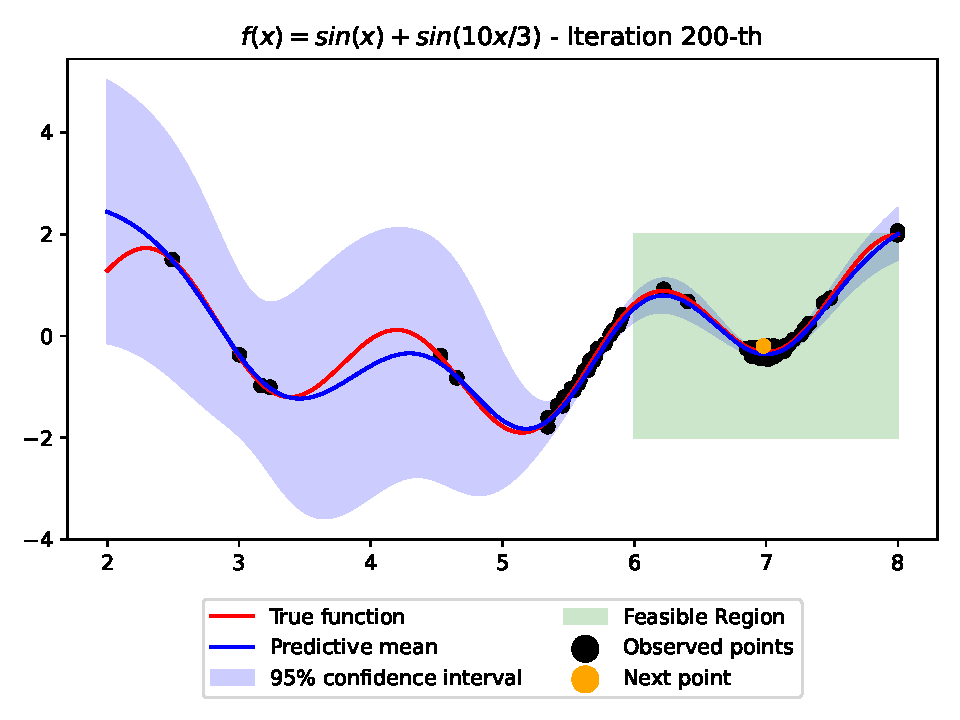
\includegraphics[width=\textwidth]{Figures/Neural-CBO/1d_toy.pdf}
    \caption{Minimization result with 1-D objective function $f(x) = \sin(x) + \sin(\frac{10x}{3})$ under the constraint $c(x) = (x-7)^2 -1 \le 0$}
    \label{fig:neural_cbo_toy_sample}
\end{figure}
In Figure \ref{fig:neural_cbo_toy_sample}, minimization result with 1-D objective function $f(x) = \sin(x) + \sin(\frac{10x}{3})$ under the constraint $c(x) = (x-7)^2 -1 \le 0$ is given to illustrate how variance formula in Eqn. \ref{Eqn:neural_cbo_variance_formula} and Alg. \ref{alg:neural_cbo} work. As shown in this figure, the variance formula performs well with relatively small values in feasible regions and larger values in infeasible regions. These results also demonstrate that the constraint model effectively guides our algorithm toward the feasible region, ensuring subsequent selection points remain within feasible regions and gradually approach the true minimum. 



\section{Theoretical Analysis}
To evaluate the performance of black-box optimization methods, much of the prior research on unconstrained \ac{bo} has focused on minimizing cumulative regret. As introduced in Section \ref{background:performance_metrics}, the cumulative regret after $T$ iterations is defined as:
\[
R_T = \sum_{t=1}^T r_t,  
\] 
where $r_t = f(\mathbf{x}_t) - f(\mathbf{x^*})$  represents the instantaneous regret, quantifying the difference between the value of the unknown function $f$ at the optimal point, $\mathbf{x}^* = \arg\max_{\mathbf{x} \in \mathcal{D}} f(\mathbf{x})$, and the value of the function at point $\mathbf{x}_t$, which is selected by the algorithm at iteration $t$. However, since $f(\mathbf{x^*})$ represents the optimal value under constraints, the algorithm may sometimes sample infeasible points with lower objective values than $f(\mathbf{x^*})$. To account for this, following \citet{xu2023constrained, nguyen2023optimistic}, we inherited the \textit{positive regret} definition as
$r_t^+ = [f(\mathbf{x}_t) - f(\mathbf{x^*})]^+,$
where $[\cdot]^+ \coloneqq \max\{0, \cdot\}$. Additionally, to measure constraint satisfaction, constraint \textit{violation} is defined as $
v_{c_i,t} = [c_i(\mathbf{x}_t)]^+$. 
Then, we introduce the \textit{cumulative positive regret} for the objective function, $R_T^+$, and the \textit{cumulative violation} for each constraint, $V_{c_i, T}$. These metrics measure the additional cost incurred due to suboptimal decisions and violations of the constraints over time by running the algorithm.  
\begin{definition} [Cumulative Positive Regret and Cumulative Violation]
    \begin{align*}
        R_T^+ &=\sum_{t=1}^T [f(\mathbf{x}_t) - f(\mathbf{x^*})]^+,
        \\
        V_{c_i, T}  &= \sum_{t=1}^T [c_i(\mathbf{x}_t)]^+, \forall i \in [K]
    \end{align*}
        
\end{definition}
\subsection{Detailed Assumptions for Objective Function and Constraints}

% \subsubsection{Assumption on black-box objective function and constraints}
We apply the general assumption stated in the Assumption \ref{assumption:rkhs} and \ref{assumption:subgaussian_noise} on both objective function and constraints:

\begin{itemize}
    \item \textbf{Objective function}: $f \in \mathcal{H}_{k_f}(\mathcal{D})$, $\norm{f}_{\mathcal{H}_{k_f}} \leq B$,  where $k_f$ is corresponding to $v(\cdot, \boldsymbol{\theta})$. The noisy observation at step $t$ is $y_t = f(\mathbf{x}_t) +  \epsilon_t$, where $\{\epsilon_i\}_{i=1}^t$ is sub-Gaussian with parameter $R_f$ and variance $\lambda_f$.

    \item \textbf{Constraint}: $c_i \in \mathcal{H}_{k_{c_i}}(\mathcal{D}), \norm{c_i}_{\mathcal{H}_{k_{c_i}}} \leq S_i$, where $k_{c_i}$ is corresponding to $u_{c_i}(\cdot, \boldsymbol{\omega}_{c_i}), \forall i = 1, \dots, K$. The noisy observation at step $t$ is $z_{c_i,t} = c_i(\mathbf{x}_t) + \eta_{c_i, t}$, where $\{\eta_{c_i, t}\}_{i=1}^t$ is sub-Gaussian with parameter $R_{c_i}$ and variance $\lambda_{c_i}$.
\end{itemize}
Now we can now state our main theorem:
\begin{restatable}{theorem}{TheoremMain}
\label{theorem:neural-cbo_main}
    Under Assumption \ref{assumption:rkhs}, Assumption \ref{assumption:subgaussian_noise} and Condition \ref{condition:network_width}, set the step size used to train the neural networks in Alg. \ref{alg:neural_cbo} as $\alpha_t \le \frac{\nu}{(T+1)^2}$, then for any $\delta \in (0,1)$,  with probability at least $1 - \delta \exp (\Omega(C^{-L} m^{1/36}))$, the Cumulative Regret $R_T$ and Cumulative Violation $V_{c_i, T}$ after $T$ iterations are bounded as:
    \begin{align*}
        & V_{c_i, T} \le 2 \beta_{c_i,T} \sqrt{\frac{S_i T}{\log(S_i+1)} (2\gamma_{c_i,T}+1)} + 2\mathcal{E}(m),
        \\
        & R_T \le R_T^+ \le 2 \beta_{f,T} \sqrt{\frac{B T}{\log(B+1)} (2\gamma_{f,T}+1)} + 2 \mathcal{E}(m),
    \end{align*}
where $\mathcal{E}(m) = \mathcal{O}(C^{2L} L^{3/2} m^{11/36})$. Especially, by choosing $m = \Omega(d^9 \exp (\nu LC^L\log T)))$, the Cumulative Regret and Cumulative Violation enjoy the  following results:
\begin{align*}
        V_{c_i, T} = \mathcal{O}(\gamma_{c_i,T} \sqrt{T}), \;\;\;\;\; R_T = \mathcal{O}(\gamma_{f,T} \sqrt{T}).
    \end{align*}
\end{restatable}
\begin{remark}
Unlike previous works \citep{zhou2020neural, zhang2021neural} that require a neural network width of \( m = \Omega(T^6) \) for convergence when modeling the objective function, our analysis builds on recent analyses from \citet{xu2024overparametrized}, which show that only a linear condition of \( m = \Omega(T) \) is needed. Furthermore, while \citet{xu2024overparametrized} focus on the input domain \( \mathbb{S}^{d-1} \), we can adapt to inputs \( \mathbf{x} \in \mathbb{R}^d \) with \( 0 < n_l < \|\mathbf{x}\| < n_b \) (where \( n_l \) and \( n_b \) are positive constants) without changing the order of \( T \) in the width condition for \( m \). Similar arguments are noted in \citep{du2018gradient, cao2020generalization}.
\end{remark}

\section{Experiments}
\label{section:neural-cbo_exp}
In this section, we outline and discuss our experimental results. We apply our method to synthetic, real-world functions. Our implementations of both problems are available at: \url{https://github.com/phantrdat/neural-cbo}.
\subsection{Experimental Setup}
\label{section:neural-cbo_baselines}
For all experiments, we compared our algorithm with well-known Constrained \ac{ei} (cEI), the extension of \ac{ei} into constrained \ac{bo} from \citet{gardner2014bayesian}. Besides, we also compare our algorithm with recent state-of-the-art algorithms in unknown constrained \ac{bo}, including ADMMBO \citep{ariafar2019admmbo}, UCB-C \citep{nguyen2023optimistic} and ConfigOpt \citep{xu2023constrained}. For our proposed Neural-CBO algorithm, we employ fully connected deep neural networks as the surrogate models for both objective function and constraints. Implementation details of our Neural-CBO algorithm as well as baselines are as follows:
\begin{itemize}
    \item  \textbf{Constrained EI} (cEI) \citep{gardner2014bayesian} integrates feasibility into the acquisition function by multiplying the probability of feasibility into EI value at every point in the search space.
    \item \textbf{ConfigOpt} \citep{xu2023constrained}: Optimize LCB-based acquisition function for the objective, which satisfies LCB-based conditions for constraints. For cEI and ConfigOpt, we used the public implementation provided at GitHub repository: \url{https://github.com/PREDICT-EPFL/ConfigOPT}.
    \item \textbf{ADMMBO} \citep{ariafar2019admmbo}: Reformulates the constrained optimization problem into an unconstrained one using the Alternating Direction Method of Multipliers (ADMM) framework. As the official implementation of ADMMBO is written in Matlab and available at \url{https://github.com/SetarehAr/ADMMBO}, we use our own Python implementation based on the official implementation.  
    \item \textbf{UCB-C} \citep{nguyen2023optimistic}: 
    Similar to ConfigOpt, but using a UCB-based acquisition function for the objective, we utilized the implementation obtained directly from the authors.
\end{itemize}
\paragraph{Neural-CBO implementation details:}
As described in Section \ref{section:neural-cbo}, the network's weights are initialized with independent samples drawn from a normal distribution $\mathcal{N} (0, 1)$. We also initialize fixed outer weight $\mathbf{q}$ to be a symmetric Bernoulli random variable with equal probability to be $-1$ or $1$. To train the surrogate neural network models, we use a Gradient Descent optimizer described in the main paper with a learning rate $\alpha = 0.001$. The network width depends on the tasks and is set to be $m = T$, where $T$ is the number of optimization iterations. We choose the network depth $L=2$ to reduce computational costs. 

\subsection{Synthetic Benchmark Functions}
\label{section:neural-cbo_synthetic}
We conducted optimization experiments on four synthetic objective functions: Branin, Ackley, Simionescu and Hartmann. The input dimension of each objective function and the corresponding number of constraints are summarized in Table \ref{tab:neural-cbo_synthetic_info}. We present the expression of each function and its constraints in the Appendix \ref{section:neural-cbo_experiments_synthetic}. 
  \begin{table}[h]
  \centering
 \caption{The input dimension and number of constraints for each synthetic objective function.}
 \vspace{0.15in}
\begin{tabular}{|c|c|c|c|c|c|}
\hline
\textbf{Obj}              & Branin & Simionescu & Ackley & Hartmann  \\ \hline
\textbf{Dim}                   & 2   & 2               & 5 & 6                  \\ \hline
\textbf{Constraints}       & 1      & 1              & 2       & 1          \\ \hline
\end{tabular}
\label{tab:neural-cbo_synthetic_info}
\end{table}
% \looseness=-1
The noise in function evaluations follows a normal distribution with zero mean, and the variance is set to 1\% of the function range. All experiments reported here are averaged over 20 runs, each with random initialization. We report the (Log10 of) the Best Positive Regret plus Violation in Figure \ref{fig:neural-cbo_synthetic}

To ensure statistical significance, we performed one-sided $t$-tests to assess whether a baseline outperforms Neural-CBO in terms of the best positive regret plus violation. The null hypothesis is $H_0: \mu_\text{baseline} \leq \mu_{\text{Neural-CBO}}$, and the alternative hypothesis is $H_a: \mu_\text{baseline} > \mu_{\text{Neural-CBO}}$, where $\mu_\text{baseline}$ and $\mu_{\text{Neural-CBO}}$ represent the means of the (Log10 of) Best Positive Regret plus Violation values of the baseline and our proposed Neural-CBO, respectively. Note that lower values indicate better performance. We present the statistical test results for four synthetic benchmark functions and two real-world tasks (described in Section \ref{section:neural-cbo_gas} and \ref{section:neural-cbo_speed}) in Table \ref{tab:neural-cbo_t-test}. Each cell in the table shows the $p$-value from the $t$-test as the first value. To account for multiple comparisons, the Benjamini-Hochberg correction was applied, with the corrected value provided as the second value. A result is labeled as ``T'' if the null hypothesis is rejected, meaning that Neural-CBO is statistically better to the compared baselines. Conversely, a result is labeled ``F'' if we cannot reject the null hypothesis, meaning that the baselines and the Neural-CBO are comparable.
\begin{table}[ht]
\caption{One-sided $t$-tests to evaluate whether the baseline outperforms Neural-CBO in terms of the best positive regret plus violation.}
  \vspace{0.15in}
\resizebox{\linewidth}{!}{
\begin{tabular}{|l|c|c|c|c|}
\hline
\multicolumn{1}{|c|}{\textbf{}} & \textbf{ConfigOpt} & \textbf{cEI}  & \textbf{UCB-C} & \textbf{ADMMBO} \\ \hline
\textbf{Branin}             & (8.25e-06, T)      & (6.41e-20, T) & (4.68e-73, T)     & (6.86e-102, T)  \\ \hline
\textbf{Simionescu}             & (6.19e-07, T)      & (2.42e-13, T) & (2.13e-25, T)  & (1.32e-78, T)   \\ \hline
\textbf{Ackley}                 & (6.95e-29, T)      & (0.13, F)      & (6.4e-97, T)   & (0.21, F)        \\ \hline
\textbf{Hartmann}               & (0.00594, T)       & (1.54e-59, T) & (4.88e-118, T) & (1.2e-87, T)    \\ 
\hline
\textbf{Gas Transmission}               & (1.52e-46, T)       & (1.78e-48, T) & (1.66e-25, T) & (1.54e-73, T)    \\ 
\hline
\textbf{Speed Reducer}               & (0.77, F)       & (6.99e-74, T) & (5.22e-77, T) & (0.38, F)    \\ 
\hline
\end{tabular}
\label{tab:neural-cbo_t-test}
}
\end{table}


\begin{figure}[h]
    \centering
   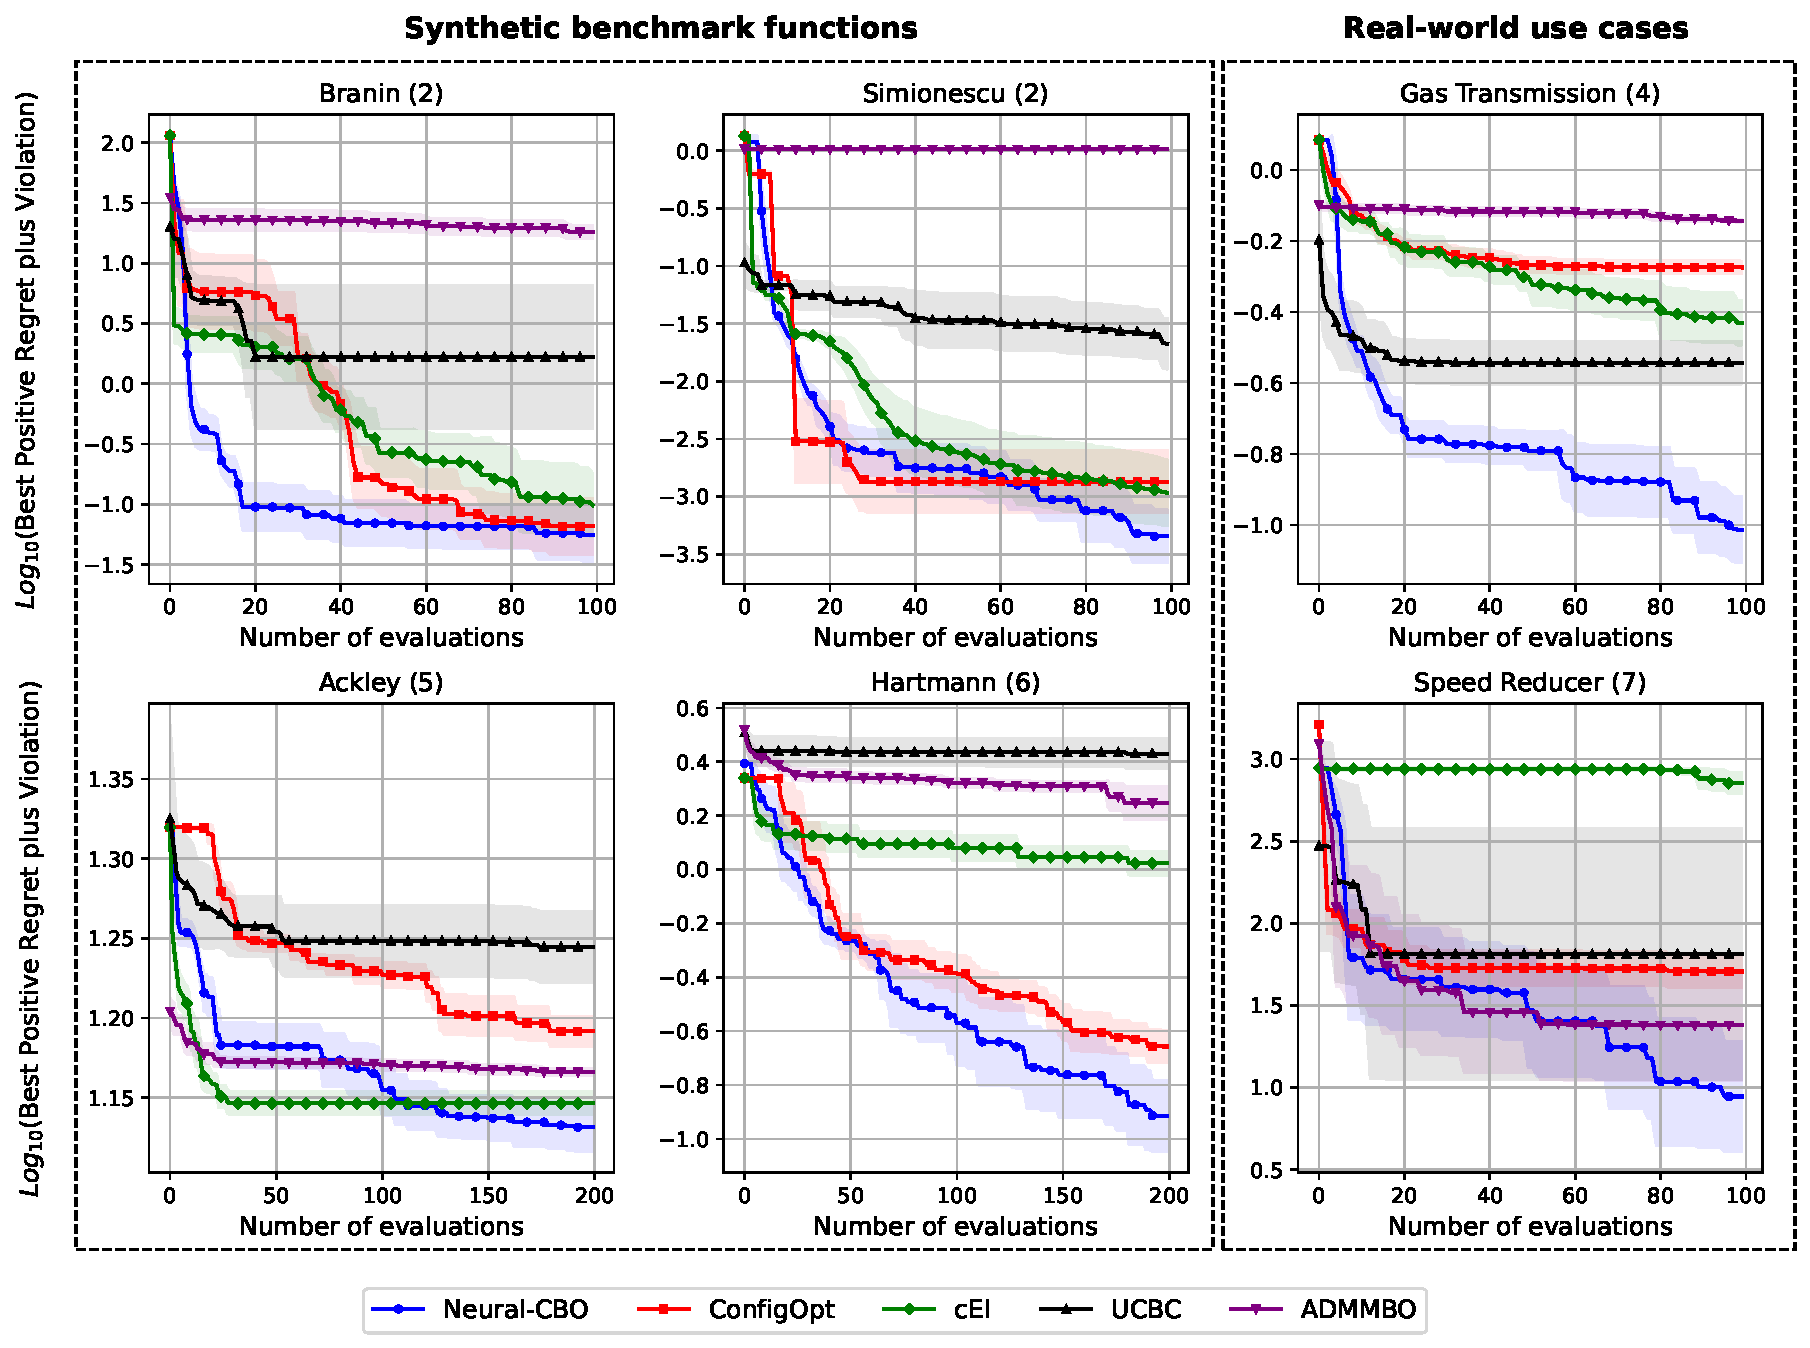
\includegraphics[width=\textwidth]{Figures/Neural-CBO/Branin-Simionescu-GasTransmission-Ackley-Hartmann-SpeedReducer.pdf}
   % \vspace{0.15in}
    \caption{The plots show (Log10 of) the Best Positive Regret plus Violation up to step $t$, which is $\min_{t \in [T]} [f(\mathbf{x}_t) - f^*]^+ + \sum_{k=1}^K [c_k(\mathbf{x}_t)]^+ ]$, comparing our proposed algorithm and four baselines. The dimension of each objective function is shown in the parenthesis. The left group is four synthetic functions introduced in Section \ref{section:neural-cbo_synthetic}, while the right group is the optimization results of Gas Transmission Compressor Design and Speed Reducer Design, described in Section  \ref{section:neural-cbo_gas} and \ref{section:neural-cbo_speed}.}
    
    \label{fig:neural-cbo_synthetic}
\end{figure}

We analyse three real-world constrained black-box optimization tasks: gas transmission compressor and speed reducer designs from \citet{kumar2020test}, and a third inspired by \citet{he2018verideep}. Details of each task will follow in the upcoming sections.  
\subsection{Gas Transmission Compressor Design}
\label{section:neural-cbo_gas}
     The main objective is to minimize operational costs or energy consumption. This requires identifying the optimal configuration of the compressor by optimizing four design variables. The problem involves $d = 4$ input dimensions and includes $K = 1$ constraint. The mathematics formula for this problem is:
    \begin{align*}
        f(\mathbf{x}) & = 8.61 \times 10^5\mathbf{x}_1^{1/2} \mathbf{x}_2\mathbf{x}_3^{-2/3} \mathbf{x}_4^{-1/2}  + 3.69 \times 10^4\mathbf{x}_3 + 7.72 \times 10^8 \mathbf{x}_1^{-1} \mathbf{x}_2^{0.219} \\
        & \;\;\; \; - 765.43 \times 10^6\mathbf{x}_1^{-1},
        \\
        \text{s.t }  c(\mathbf{x}) &= \mathbf{x}_4\mathbf{x}_2^{-2} + \mathbf{x}_2^{-2} - 1 \le 0
    \end{align*}

    
 \subsection{Speed Reducer Design}
\label{section:neural-cbo_speed}
This task involves designing a speed reducer for a small aircraft engine, focusing on minimizing weight while meeting several constraints, including bending stress on gear teeth, surface stress, transverse deflections of shafts, and shaft stresses. The problem includes 7 decision variables and 11 constraints, resulting in an input dimension of $d=7$ and $K=11$ constraints and can be formulated as:
\begin{align*}
    f(\mathbf{x}) &= 0.7854\mathbf{x}_2
^2 \mathbf{x}_1(14.9334\mathbf{x}_3 - 43.0934 + 3.3333\mathbf{x}_3^2) 
\\
    & \;\;\;\; +0.7854(\mathbf{x}_5\mathbf{x}_7^2 + \mathbf{x}_4\mathbf{x}_6^2) - 1.508\mathbf{x}_1(\mathbf{x}_7^2 + \mathbf{x}_6^2) + 7.477(\mathbf{x}_7^3 + \mathbf{x}_6^3), 
    \\
    \text{s.t. } & \begin{cases} 
    c_1(\mathbf{x}) = -\mathbf{x}_1\mathbf{x}_2^2\mathbf{x}_3 + 27  & \le 0 
    \\
    c_2(\mathbf{x}) = -\mathbf{x}_1\mathbf{x}_2^2\mathbf{x}_3^2 + 397.5 & \le 0 
    \\
    c_3(\mathbf{x}) = -\mathbf{x}_2\mathbf{x}_6^4
    \mathbf{x}_3\mathbf{x}_4^{-3}+ 1.93 &\le 0 
    \\
    c_4(\mathbf{x}) = -\mathbf{x}_2\mathbf{x}_7^4
    \mathbf{x}_3\mathbf{x}_5^{-3}+ 1.93 & \le 0 
    \\
    c_5(\mathbf{x}) = 10\mathbf{x}_6^{-3} \sqrt{16.91 \times 10^6 + (745\mathbf{x}_4\mathbf{x}_2^{-1}
    \mathbf{x}_3^{-1}
    )^2} -1100 & \le 0
    \\
    c_6(\mathbf{x}) = 10\mathbf{x}_7^{-3} \sqrt{157.5 \times 10^6 + (745\mathbf{x}_5\mathbf{x}_2^{-1}
    \mathbf{x}_3^{-1}
    )^2} - 850 & \le 0
    \\
    c_7(\mathbf{x}) = \mathbf{x}_2\mathbf{x}_3 -40 & \le 0 
    \\
    c_8(\mathbf{x}) = -\mathbf{x}_1 \mathbf{x}_2^{-1} + 5 & \le 0
    \\
    c_9(\mathbf{x}) = -\mathbf{x}_1 \mathbf{x}_2^{-1} - 12  & \le 0
    \\
    c_{10}(\mathbf{x}) = 1.5\mathbf{x}_6 - \mathbf{x}_4  + 1.9  & \le 0
    \\
    c_{11}(\mathbf{x}) = 1.1\mathbf{x}_7 - \mathbf{x}_5  + 1.9  & \le 0
    \\
    \end{cases},
\end{align*}

We report numerical results of Section \ref{section:neural-cbo_gas} and  \ref{section:neural-cbo_speed} in Figure \ref{fig:neural-cbo_synthetic} and Table \ref{tab:neural-cbo_t-test}.
\subsection{Designing Sensitive Samples for Model Tampering Detection}
\label{section:neural-cbo_sensitive_sample}


We build on the sensitive sample generation example described in Section \ref{section:neural-bo_sensitive_samples} to address an additional practical challenge: incorporating constraints on the generated samples to ensure their realism. Specifically, in scenarios where tampered machine learning models are hosted on cloud services, attackers may attempt to bypass detection by modifying models while keeping their behavior on plausible inputs unchanged. To prevent attackers from evading detection, sensitive samples must resemble normal inputs. Therefore, a human-in-the-loop process is employed, where reviewers rate the realism of each sample on a scale of $(0,1)$; higher scores indicate more realistic samples. These scores serve as constraints in the optimization, where obtaining human feedback can be costly. Assuming a pre-trained model $s_\varphi(\mathbf{x})$ may have been altered after being uploaded, the goal is to find sensitive samples by solving the optimization problem: 
\begin{align*}
    v &= \argmax_\mathbf{x} \norm{\frac{\partial s_\varphi(\mathbf{x})}{\partial \varphi}}_F 
    \\
    \text{s.t. } &  realistic(v) \ge h, 
\end{align*}
where $\norm{\cdot}_F$ denotes the Frobenius norm, $realistic(\cdot)$ is the human-based scoring function and $h$ is a pre-defined threshold. A detection is \emph{successful} if at least one of the $N_S$ sensitive samples shows a different top-1 prediction between the tampered and original models.  

We employed the same experimental setup outlined in Section \ref{section:neural-bo_sensitive_samples}, using a pre-trained MNIST handwritten digit classification model and compared our method's performance against several baselines based on average detection rates for sensitive samples. The model was tampered with by adding noise to its weights 1,000 times, producing 1,000 distinct versions. While the original model had a top-1 accuracy of 93\%, this dropped to $87.73\% \pm 0.08\%$ after tampering. To reduce computational costs, we downscaled the images from $28 \times 28$ to $7 \times 7$, optimized in this 49-dimensional space, and then restored them to the original resolution to generate sensitive samples. Feasible samples were chosen based on their realistic scores. Figure \ref{fig:neural-cbo_sensitive_sample} shows the detection rates of (feasible) sensitive samples generated by our method compared to four baselines, demonstrating that our samples achieved higher detection rates. As expected, the detection rate improves with more samples and our method is consistently competitive.



\begin{figure}[H]
    \centering
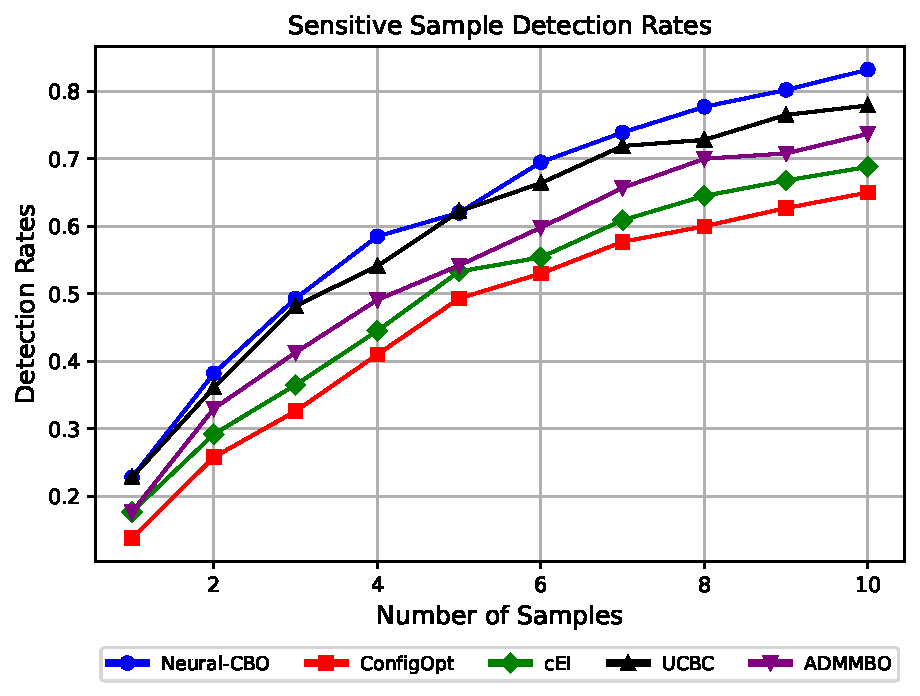
\includegraphics[width=\textwidth]{Figures/Neural-CBO/sensitive_sample_detection_rate.pdf}
    \caption{Detection Rates w.r.t to the number of samples for the MNIST dataset. As shown in the figure, Neural-CBO can generate sensitive samples that achieve nearly 85\% of the detection rate with just 10 samples.}
    \label{fig:neural-cbo_sensitive_sample}
\end{figure}



\section{Conclusion}
We proposed a novel algorithm for black-box optimization with unknown constraints, utilizing deep neural networks as surrogate models for both the objective function and constraints. Our algorithm leverages the bounded nature of constraint values by applying LCB conditions at each iteration to ensure feasibility. We also employ EI as the acquisition function to balance exploration and exploitation, especially in scenarios where feasible regions are significantly smaller than the search space. Our theoretical analysis shows that, under mild conditions regarding neural network width, our algorithm achieves upper bounds on cumulative regret and constraint violations comparable to previous GPs-based methods. We validate our approach through experiments on synthetic and real-world benchmark tasks involving structural data, with results demonstrating competitive performance against state-of-the-art methods.

% as our baseline and tampered it by adding noise to each weight 1,000 times, resulting in 1,000 distinct models. The original model had a top-1 accuracy of $93\%$, which dropped to $87.73\% \pm 0.08\%$ after tampering. To reduce computational costs, we downscaled the images from $28 \times 28$ to $7 \times 7$, optimizing in this 49-dimensional space. After identifying the optimal points, we restored them to the original resolution to generate sensitive samples.
 
\chapter{PINN-BO: A Black-Box Optimization
Algorithm Using Physics-Informed
Neural Networks} % Main chapter title
\label{chap:pinn-bo}
\section{Introduction}

In many scientific and engineering problems, the behavior of systems is often described by mathematical equations called \acfp{pde}. These equations represent fundamental physical laws, such as how heat spreads over time (the heat equation) or how fluids flow while considering factors like viscosity and external forces (the Navier-Stokes equations). \acp{pde} are essential tools in various fields, including structural analysis and electromagnetic, showing their broad importance.

Recently, researchers have tried to use \acp{pde} to improve the accuracy of modelling unknown functions. A common method uses \acp{gp} to combine information from observations of the objective function with the knowledge provided by \acp{pde}. While \acp{gp} are effective, they become slow and impractical for large datasets because their computations involve inverting large matrices, which can be very time-consuming.

To solve these challenges, \acfp{pinn} have been introduced. \acp{pinn} use neural networks to capture complex and nonlinear relationships, making them more flexible and scalable than \acp{gp}. \acp{pinn} can handle a wide variety of \acp{pde}, including nonlinear ones, and are better suited for large-scale problems in science and engineering.

While \acp{pde} offer useful information that can make optimization more efficient by reducing the need for expensive evaluations of the objective function. However, there is still limited research on how to effectively use \acp{pde} in \ac{bo}, where the objective function is unknown, noisy, or difficult to evaluate.

This chapter presents PINN-BO, a black-box optimization framework that employs a \ac{pinn} to model the unknown function, incorporates physical knowledge expressed by \acp{pde} constraints into the optimization process. Hence, PINN-BO aims to enhance model accuracy and improve constraint handling, particularly in problems governed by established physical laws. We summarize \textbf{the contributions of this chapter} as follows:
\begin{itemize}
    \item We introduce a novel black-box optimization problem with physics information, described by \acfp{pde}, which is used to govern the objective function.
    
    \item We propose PINN-BO, a black-box optimization algorithm employing \acl{pinn} with \acfp{pde} induced by natural laws to perform efficient optimization, bringing several benefits: improved sample-efficiency of optimization, scalable computation that only grows linearly with the number of function evaluations, and the ability to incorporate a broad class of \acp{pde}.
     
    \item We provide a theoretical analysis of our proposed PINN-BO algorithm to illustrate that incorporating linear \acp{pde} can lead to $\mathcal{O}\left(\sqrt{T\gamma_T}\sqrt{\gamma_T - I (f; \mathbf{Y}_T; \mathbf{U}_r) } \right)$ regret, where $T$ is the number of black-box function evaluations and $I (f; \mathbf{Y}_T; \mathbf{U}_r)$ is interaction information between the black-box function  $f$, its observations $\mathbf{Y}_T$ and the \ac{pde} data $\mathbf{U}_r$ (see Section \ref{section:pinn-bo_theoretical_analysis}).
    
    \item We perform experiments with a variety of tasks showing that our algorithm outperforms current state-of-the-art black-box optimization methods.
\end{itemize} 
This chapter begins by introducing the problem setting and give an example to illustrate our proposed setting, followed by a detailed description of the PINN-BO framework and its theoretical analysis.
 % For referencing the chapter elsewhere, use \ref{chap:background}
\section{Problem Setting}
\label{section:pinn-bo_problem_setting}
In this chapter, we consider a global optimization problem setting where the objective function $f \colon \mathcal{D} \rightarrow \mathbb{R}$ is associated with a \ac{pde}:   
\begin{equation*}
        \underset{\mathbf{x} \in \mathcal{D}}{\min} f(\mathbf{x}) \text{ s.t. }  \mathcal{N}[f](\mathbf{x}) = g(\mathbf{x}),
\end{equation*} 
where $\mathcal{D} \subset \mathbb{R}^d$ is a $d$-dimensional bounded domain and $\mathcal{N}[f]$ denotes a differential operator of the function $f$ with respect to the input $\mathbf{x}$. The function $f$ is an expensive, black-box function, and its evaluations are obtainable only through noisy measurements in the form of $y = f(\mathbf{x}) + \epsilon$, where $\epsilon$ represents sub-Gaussian noise. Additionally, the function $g(\mathbf{x})$ is a cheap-to-evaluate function, which may also involve noise, with respect to the \ac{pde}-constraint. Furthermore, it is assumed that the \textbf{boundary conditions} of the PDEs are either \textit{unknown or inaccessible}.
\begin{remark}
    Considering the damped harmonic oscillator from classical physics as a real-world example where $f(x)$ is the displacement of the oscillator as a black-box function of time $x$, and measuring the displacement of a damped harmonic oscillator accurately can be expensive due to several factors, e.g., instrumentation cost, environmental factors, and calibration requirements. This displacement is governed by the \ac{pde}: $m \frac{d^2f}{dx^2} + c \frac{df}{dx} + kf = 0$, where $\mathcal{N}[f](x) = m \frac{d^2f}{dx^2} + c \frac{df}{dx} + kf$, $g(x)=0$, $m, c, k$ are mass, damping and spring values, respectively. 
\end{remark}
\begin{remark}
    Assumptions about the \textit{unknown} or \textit{inaccessible} nature of boundary conditions are widely applicable across many problem settings. As an example, \citet{cai2020heat} examines a two-dimensional heat transfer problem with forced heat convection around a circular cylinder. The heat measurement entails high costs due to the material, size, and shape of the system. The problem has known incompressible Navier-Stokes and heat transfer equations. However, the thermal boundary conditions are difficult to ascertain precisely because of the complex and large instruments. The unavailability of these boundary conditions prevents the straightforward solution of the underlying function $f$ using traditional numerical techniques.
\end{remark}


\section{Proposed PINN-BO Method}
In this section, we present our proposed \ac{pinn} based \acl{bo} (PINN-BO). PINN-BO algorithm combines optimization and machine learning techniques to efficiently optimize an unknown black-box function over a given input space while leveraging physics-informed constraints described by a \ac{pde}. Following the fundamental principles of Bayesian optimization, our algorithm consists of two primary steps: (1) constructing a model of the black-box objective function, and (2) employing this model to select the next function evaluation point during each iteration. In the first step, our approach diverges from traditional Bayesian Optimization algorithms that typically utilize \acfp{gp} to model the objective function. Instead, we employ a fully connected neural network denoted as $h(\mathbf{x}; \boldsymbol{\theta})$ to learn the function $f$ as follows:
\[
h(\mathbf{x};\boldsymbol{\theta}) = \frac{1}{\sqrt{m}} \mathbf{W}_L \psi(\mathbf{W}_{L-1}\psi(\cdots \psi(\mathbf{W}_1 \mathbf{x})),
\]
where $\psi\colon \mathbb{R} \rightarrow \mathbb{R}$ is a coordinate-wise smooth activation function (e.g., ReLU, Tanh), $\mathbf{W}_1 \in \mathbb{R}^{m \times d}, \mathbf{W}_i \in \mathbb{R}^{m \times m}, 2\leq i \leq L-1, \mathbf{W}_L \in \mathbb{R}^{1 \times m}$, and $\boldsymbol{\theta} \in \mathbb{R}^p$ is the collection of parameters of the neural network, $p=md+m^2(L-2)+m$ and $d$ is the dimension of inputs, i.e., $\mathbf{x} \in \mathcal{D} \subset \mathbb{R}^d$. We initialize all the weights to be independent and identically distributed as standard normal distribution $\mathcal{N}(0,1)$ random variables. To leverage the information embedded within the \ac{pde} governing the objective function $f$, our algorithm generates a set of $N_r$ \ac{pde} data points denoted as $\mathcal{R} =  \{\mathbf{z}_j, u_j\}_{j=1}^{N_r}$. Here, $u_j$ represents the noisy evaluations of the function $g$ at the corresponding point $\mathbf{z}_j$, where $u_j = g(\mathbf{z}_j) + \eta_j$. Besides, we denote $\mathcal{D}_t = \{\mathbf{x}_i, y_i\}_{i=1}^t$ as the set of noisy observations of the unknown function $f$ after $t$ optimization iterations, where $y_t = f(\mathbf{x}_t) + \epsilon_t$. We further define some other notations:
\begin{equation*}
        \phi(\cdot) = \nabla_{\boldsymbol{\theta}} h(\cdot; \boldsymbol{\theta}_0) ; \; \; \; \;
        \omega(\cdot)  = \nabla_{\boldsymbol{\theta}} \mathcal{N}[h] (\cdot; \boldsymbol{\theta}_0)\\
\end{equation*}
where $\phi(\cdot)$ is the gradient of $h(\cdot; \boldsymbol{\theta}_0)$ with respect to the parameter $\boldsymbol{\theta}$, evaluated at initialization $\boldsymbol{\theta}_0$. Similarly, $\omega(\cdot)$ represents the gradient of $\mathcal{N}[h](\cdot; \boldsymbol{\theta}_0)$ with respect to model parameters $\boldsymbol{\theta}$ and evaluated at initialization $\boldsymbol{\theta}_0$, where $\mathcal{N}[h](\cdot; \boldsymbol{\theta}_0)$ is the result of applying differential operator $\mathcal{N}$ (with respect to the input) to $h(\cdot; \boldsymbol{\theta}_0)$. In our paper, we focus on cases where the differential operator \( \mathcal{N} \), when applied to a \textit{real-valued} function \( h \), produces another \textit{real-valued} function \( \mathcal{N}[h] \) (e.g., linear differential operator with real constant coefficients). 

Both $\mathcal{D}_t$ and $\mathcal{R}$ play an important role in the subsequent stages of the algorithm, specifically in the minimization of the loss function associated with learning the network $h(\mathbf{x}, \boldsymbol{\theta}_t)$ at optimization iteration $t$:
\begin{equation}
    \label{eqn:pinn_loss}
    \resizebox{0.9\textwidth}{!}{
$\mathcal{L}(t) = \sum^{t-1}_{i=1} [y_i - \nu_t h(\mathbf{x}_i; \boldsymbol{\theta}_{t-1})]^2 + \sum^{N_r}_{j=1}[u_j - \nu_t \mathcal{N}[h](\mathbf{z}_j; \boldsymbol{\theta}_{t-1})]^2$,
}
\end{equation}
where $\nu_t$ is a scale parameter that controls the exploration-exploitation trade-off. 

For the second step, we employ a greedy strategy to pick the next sample point $\mathbf{x}_t$. At each iteration $t$, the algorithm updates the neural network by optimizing the loss function described in Eqn \ref{eqn:pinn_loss} by gradient descent, with scaled function value predictions $\nu_t h(\cdot; \boldsymbol{\theta}_{t-1})$ and scaled predictions with respect to the governed \ac{pde} $\nu_t \mathcal{N}[h](\cdot; \boldsymbol{\theta}_{t-1})$. In the proof of Section \ref{section:pinn-bo_theoretical_analysis}, we show this action is equivalent to placing the \ac{gp} prior over function values $f_{1:t}$ and \ac{pde} values $g_{1:N_r}$ (Corollary \ref{corollary:pinn-bo_PINN_GP_func} in Appendix \ref{section:pinn-bo_supp}). 

The posterior distribution of the function prediction $\widetilde {f}_t(\mathbf{x}) = h(\mathbf{x}, \boldsymbol{\theta}_{t-1})$ at a new data point $\mathbf{x}$ can be viewed as being sampled from a \ac{gp} with specific posterior mean and variance function (Lemma \ref{lemma:pinn-bo_PINN_mean_cov}). This allows us to directly use the network prediction as an acquisition function following the principle of \acl{ts}.

The next evaluation point $\mathbf{x}_t$ is selected by minimizing this acquisition function $\widetilde {f}_t(\mathbf{x}) = h(\mathbf{x}, \boldsymbol{\theta}_{t-1})$. Then, the black-box function is queried at point $\mathbf{x}_t$, resulting in a (noisy) observation $y_t$, which is subsequently used to update the dataset $\mathcal{D}_t$. The \ac{pde} observations set $\mathcal{R}$, in combination with the observations in $\mathcal{D}_t$, is integrated into the training process of the neural network by minimizing the squared loss, as described in Eqn \ref{eqn:pinn_loss}. We provide a concise step-by-step summary of our approach in Algorithm \ref{alg:PINN-BO}.

To enhance the exploration step, it is important to bring the additional information to improve our model of objective function, especially in the regions where the optima are likely to be located. In our case, this task of exploration is easier as we have access to \ac{pde} which provides knowledge about the objective function and reduces the amount of information that is needed to model the function. In Section \ref{section:pinn-bo_theoretical_analysis} (Theoretical Analysis), we derive a scaling factor $\nu_t = B + \widetilde{R} \sqrt{2\gamma_t - 2 I(f; \mathbf{Y}_t; \mathbf{U}_r)  + \log(\frac{1}{\delta})}$,  which directly reflects this intuition. It reduces the maximum information gain  (which can be thought of as the complexity of the function modeling) by the interaction information $I(f; \mathbf{Y}_t; \mathbf{U}_r)$, which is a generalization of the mutual information for three variables: unknown function $f$,  its observations $\mathbf{Y}_t$, and the \ac{pde} data $\mathbf{U}_r$. This information can be calculated as $I(f; \mathbf{Y}_t; \mathbf{U}_r) = \frac{1}{2}  \log (\frac{\det(\frac{\boldsymbol{\Phi}_t^\top \boldsymbol{\Phi}_t}{\lambda_1} + \mathbf{I})\det(\frac{\boldsymbol{\Omega}_r^\top \boldsymbol{\Omega}_r}{\lambda_2} + \mathbf{I})}{\det(\frac{\boldsymbol{\Phi}_t^\top \boldsymbol{\Phi}_t}{\lambda_1} + \frac{\boldsymbol{\Omega}_r^\top \boldsymbol{\Omega}_r}{\lambda_2} + \mathbf{I})}) $, where $\boldsymbol{\Phi}_t  = [\phi(\mathbf{x}_1)^\top,\dots, \phi(\mathbf{x}_t)^\top ]$ and 
$\boldsymbol{\Omega}_r  = [\omega(\mathbf{z}_1)^\top, \dots, \omega(\mathbf{z}_{N_r})^\top ]$. The value of $\nu_t$ signifies how our algorithm continues the exploration in regions of search space where the function $f$ has no implicit knowledge through \ac{pde} observations. These are the regions indicated by $\gamma_t - I(f; \mathbf{Y}_t; \mathbf{U}_r)$, which is the amount of information about the unknown function $f$ remains after our algorithm interacts with \ac{pde} data $\mathbf{U}_r$.  

\begin{algorithm}[!ht]
\caption{Physics-informed Neural Network based Black-box optimization (PINN-BO)}
\label{alg:PINN-BO}
\textbf{Input}: The input space $\mathcal D$, the optimization budget $T$, \ac{pde} training set size $N_r$, $\delta \in (0,1)$, parameters $B, R_1, R_2, \lambda_1, \lambda_2$ (see Assumption \ref{assumption:pinn-bo_subgaussian} and \ref{assumption:pinn-bo_rkhs} in Section \ref{section:pinn-bo_theoretical_analysis}).
\begin{algorithmic}[1]
\State Initialize $\mathcal{D}_0 = \emptyset$ and $\boldsymbol{\theta}_0 \sim \mathcal{N}(\mathbf{0},\mathbf{I})$ 
\State Generate set $\mathcal{R} = \{\mathbf{z}_j, u_j\}_{j=1}^{N_r}$ from the \ac{pde}.

\For{$t = 1$ to $T$}
\State Set $\nu_t = B + \widetilde{R} \sqrt{2\gamma_t - 2 I(f; \mathbf{Y}_t; \mathbf{U}_r)  + \log(\frac{1}{\delta})}$, where $\widetilde{R} = \sqrt{\left(\frac{R_1}{\lambda_1}\right)^2 + \left(\frac{R_2}{\lambda_2}\right)^2}$. 
\State $\widetilde{f_t}(\mathbf{x}) = h(\mathbf{x}; \boldsymbol{\theta}_{t-1})$ 
\State Choose $\mathbf{x}_t = \argmin_{\mathbf{x} \in \mathcal{D}} \widetilde{f_t}(\mathbf{x}) $ and receive observation $y_t = f(\mathbf{x}_t) + \epsilon_t$
\State Update $\mathcal{D}_t = \mathcal{D}_{t-1} \cup \{\mathbf{x}_t, y_t\}$
\State Update $ \boldsymbol{\theta}_t = \argmin_{\boldsymbol{\theta}} \mathcal{L}(\boldsymbol{\theta})$ using Eqn. \ref{eqn:pinn_loss} by gradient descent with $\nu = \nu_t$.
\EndFor
\end{algorithmic}
\end{algorithm}


\section{Theoretical Analysis}
\label{section:pinn-bo_theoretical_analysis}

In this section, we provide a regret bound for the proposed PINN-BO algorithm. As presented in Section \ref{background:performance_metrics}, to quantify the algorithm's regret, we employ the cumulative regret, defined as $R_T = \sum_{t=1}^T r_t$ after $T$ iterations. Here, $\mathbf{x}^* = \argmin_{\mathbf{x} \in \mathcal{D}} f(\mathbf{x})$ represents the optimal point of the unknown function $f$, and $r_t = f(\mathbf{x^*}) - f(\mathbf{x}_t)$ denotes the instantaneous regret incurred at time $t$. Our regret analysis is built upon the recent NTK-based theoretical work of \citet{wang2022and} and proof techniques of GP-TS in \citet{chowdhury2017kernelized}. Before proceeding with the theoretical analysis, we now introduce a set of definitions and assumptions. They clarify our proof and set up the basis and conditions for our analysis. \textbf{A detailed proof can be found in Section \ref{section:pinn-bo_theoretical_analysis} of the Appendix.}   
\begin{definition}
    We define matrix $\mathbf{K}_\mathrm{NTK-PINN}$ as  the \textit{neural tangent kernel of a Physics-Informed Neural Network (NTK of PINNs)}: 
\begin{equation}
\renewcommand\arraystretch{1.2}
    \label{definition:PINN-NTKs}
\mathbf{K}_\mathrm{NTK-PINN} = 
\begin{bmatrix}
    \mathbf{K}_{uu} & \mathbf{K}_{ur} \\
    \mathbf{K}_{ru} & \mathbf{K}_{rr}
\end{bmatrix},
\end{equation}
where $(\mathbf{K}_{uu})_{ij} = \langle \phi(\mathbf{x}_i), \phi(\mathbf{x}_j) \rangle, 
 (\mathbf{K}_{ur})_{ij} = \langle \phi(\mathbf{x}_i), \omega(\mathbf{z}_j) \rangle, (\mathbf{K}_{rr})_{ij} = \langle \omega(\mathbf{z}_i), \omega(\mathbf{z}_j) \rangle$ and $\mathbf{K}_{ru} = \mathbf{K}_{ur}^\top$, defined using $\mathcal{D}_t$ and $\mathcal R$. 
\end{definition}

 \begin{assumption}
 \label{assumption:pinn-bo_subgaussian}
 We assume the noises $\{\epsilon_i\}_{i=1}^T$ where $\epsilon_i = y_i - f(\mathbf{x}_i)$ and $\{\eta_j\}_{j=1}^{N_r}$ where $\eta_j = u_j - g(\mathbf{z}_j)$  are conditionally sub-Gaussian with parameter $R_1 > 0$ and $R_2 >0$, where $\{\epsilon_i\}_{i=1}^T$ and $\{\eta_j\}_{j=1}^{N_r}$ is assumed to capture the noises induced by querying the black-box, expensive function $f(\cdot)$  and cheap-to-evaluate \ac{pde}-related function $g(\cdot)$ respectively. 
 \begin{equation*}
     \begin{split}
         \forall i \ge 0, & \; \forall \lambda_1 \in \mathbb{R}, \;  \mathbb{E}[e^{\lambda_1\epsilon_i} \rvert \mathcal{F}_{t-1}] \le e^\frac{\lambda_1^2 R_1^2}{2} \\
         \forall j \ge 0, & \; \forall \lambda_2 \in \mathbb{R}, \;  \mathbb{E}[e^{\lambda_2\eta_j} \rvert \mathcal{F}_{N_r-1}^\prime] \le e^\frac{\lambda_2^2 R_2^2}{2}
     \end{split}
 \end{equation*}
where $\mathcal{F}_{t-1}, \mathcal{F}_{N_r-1}^\prime$ are the $\sigma$-algebra generated by the random variables $\{\mathbf{x}_i, \epsilon_i\} 
^{t-1}_{i=1} \cup \{\mathbf{x}_t\}$ and $\{\mathbf{z}_j, \eta_j\} 
^{N_r-1}_{j=1} \cup \{\mathbf{z}_{N_r}\}$, respectively.
 \end{assumption}
 \begin{assumption}
    \label{assumption:pinn-bo_rkhs}
     We assume $f$ to be an element of the \acf{rkhs} associated with real-valued functions defined on the set $\mathcal{D}$ (For more details about \ac{rkhs}, see Section \ref{background:rkhs}). This specific \ac{rkhs} corresponds to the \acf{ntk} of a physics-informed neural network (NTK-PINN) and possesses a bounded norm denoted as $\norm{f}_{\mathcal{H}_{k_\textup{NTK-PINN}}} \leq B$.  Formally, this \ac{rkhs} is denoted as $\mathcal{H}_{k_\textup{NTK-PINN}}(\mathcal D)$, and is uniquely characterized by its kernel function $k_\textup{NTK-PINN}(\cdot, \cdot)$. The \ac{rkhs} induces an inner product $\langle \cdot, \cdot \rangle$ that obeys the reproducing property:
    $f(\mathbf{x}) = \langle f, k_\textup{NTK-PINN}(\cdot, \mathbf{x})\rangle$ for all $f \in  \mathcal{H}_{k_\textup{NTK-PINN}}(\mathcal{D})$. 
    The norm induced within this \ac{rkhs}, $\norm{f}_{\mathcal{H}_{k_\textup{NTK-PINN}}} = \sqrt{\langle f,f\rangle_{\mathcal{H}_{k_\textup{NTK-PINN}}}}$, quantifies the smoothness of $f$ concerning the kernel function $k_\textup{NTK-PINN}$, and satisfies: $f \in \mathcal{H}_{k_\textup{NTK-PINN}}(\mathcal{D})$ if and only if $\norm{f}_{k_{\mathcal{H}_\textup{NTK-PINN}}} < \infty$. 
 \end{assumption}


Assumptions \ref{assumption:pinn-bo_subgaussian} and \ref{assumption:pinn-bo_rkhs} represent commonly employed and well-established assumptions in GP-based Bandits and Bayesian Optimization \citep{chowdhury2017kernelized,vakili2021optimal}. We are now prepared to establish an upper bound on the regret incurred by our proposed PINN-BO algorithm.  

We begin by presenting key lemmas for establishing the regret bound in Theorem \ref{theorem:pinn-bo_regret_bound} of the proposed algorithms. The following lemma demonstrates that, given the assumption of an infinitely wide network, the output of the trained physics-informed neural network used to model the unknown function $f$ governed by a linear \ac{pde}, after running $t$ optimization iterations in Algorithm \ref{alg:PINN-BO}, can be regarded as sampling from a \ac{gp} with specific mean and covariance functions.
\begin{restatable}{lemma}{PinnMeanCov} 
\label{lemma:pinn-bo_PINN_mean_cov}
Conditioned on $\mathcal{D}_t = \{\mathbf{x}_i, y_i\}_{i=1}^t, \mathcal{R} = \{\mathbf{z}_j, u_j\}_{j=1}^{N_r}$, the acquisition function $\widetilde{f}_t(\mathbf{x}) = h(\mathbf{x}; \boldsymbol{\theta}_{t-1})$ can be viewed as a random draw from a $\mathrm{GP}\left(\mu_{t}^f (\mathbf{x}), \nu_t^2 \left(\sigma^f_t\right)^2(\mathbf{x})\right)$ with the following mean and covariance functions:
\begin{equation*}
\begin{split}
     \mu_{t}^f (\mathbf{x}) &= \phi(\mathbf{x})^\top \boldsymbol{\xi}_t^\top \mathbf{\widehat{K}}_\mathrm{PINN}^{-1} 
     \renewcommand\arraystretch{1.2}
     \begin{bmatrix}
         \mathbf{Y}_t \\
         \mathbf{U}_r
     \end{bmatrix} \\
    \left(\sigma^f_t\right)^2(\mathbf{x}) &=  \langle \phi(\mathbf{x}),  \phi(\mathbf{x}) \rangle - \phi(\mathbf{x})^\top \boldsymbol{\xi}_t^\top \mathbf{\widehat{K}}_\mathrm{PINN}^{-1} \boldsymbol{\xi}_t \phi(\mathbf{x}), \\
\end{split}
\end{equation*}
where 
\begin{equation*}
    \renewcommand\arraystretch{1.2}
    \begin{split}
\mathbf{\widehat{K}}_\mathrm{PINN}^{-1} &=  
    \begin{bmatrix}
    \mathbf{K}_{uu} + \lambda_1 \mathbf{I} & \mathbf{K}_{ur} \\
    \mathbf{K}_{ru} & \mathbf{K}_{rr} + \lambda_2 \mathbf{I}
    \end{bmatrix} ^{-1}  = \begin{bmatrix}
    \widetilde{\mathbf{A}} & \widetilde{\mathbf{B}} \\
    \widetilde{\mathbf{C}} & \widetilde{\mathbf{D}}
    \end{bmatrix}\\
    \boldsymbol{\Phi}_t & = [\phi(\mathbf{x}_1)^\top,\dots, \phi(\mathbf{x}_t)^\top ]  
\\
    \boldsymbol{\Omega}_r & = [\omega(\mathbf{z}_1)^\top, \dots, \omega(\mathbf{z}_{N_r})^\top ] \\ 
 \boldsymbol{\xi}_t &= \begin{bmatrix}
    \boldsymbol{\Phi}_t^\top & \boldsymbol{\Omega}_r^\top  
    \end{bmatrix}^\top 
\\
    \mathbf{K}_{uu} &= \boldsymbol{\Phi}_t \boldsymbol{\Phi}_t^\top, \;  \mathbf{K}_{ur} = \boldsymbol{\Phi}_t \boldsymbol{\Omega}_r^\top, \;
    \mathbf{K}_{ru} = \mathbf{K}_{ur}^\top, \mathbf{K}_{rr} = \boldsymbol{\Omega}_r \boldsymbol{\Omega}_r^\top 
\\
    \mathbf{Y}_t &= [y_1, y_2, \dots, y_t]^\top, 
    \mathbf{U}_r = [u_1, u_2, \dots, u_{N_r}]^\top \\
    \end{split}
\end{equation*}
\end{restatable}

Generic \ac{bo} methods (without the extra information from \ac{pde}) utilized the \textit{maximum information gain} over search space $\mathcal{D}$ at time $t$:
    $\gamma_t := \max_{\mathcal{A} \subset \mathcal{D}: \lvert \mathcal{A} \rvert=t} I(\mathbf{Y}_\mathcal{A}, f_\mathcal{A})$, 
    where $I(\mathbf{Y}_\mathcal{A}, f_\mathcal{A})$ denotes the mutual information between $f_\mathcal{A} = [f(\mathbf{x})]_{\mathbf{x}\in \mathcal{A}}$ and noisy observations $\mathbf{Y}_\mathcal{A}$, which quantifies the reduction in uncertainty about the objective function $f$ after observing $y_A$. The maximum information gain is the fundamental component when analyzing regret bound for their algorithm \citep{srinivas2009gaussian,vakili2021optimal}. Further details on this concept can be found in Section \ref{section:MIG}. However, in our work, the \ac{pde} evaluations $\{u_j\}_{j=1}^{N_r}$ of the function $g$ is considered as the second source of information that contributes to reduce the uncertainty of $f$. Therefore, we introduce the \textit{interaction information} as the generalization of \textit{mutual information} for three random variables:
\begin{definition}
\label{def:pinn-bo_interaction_information}
The \textbf{interaction information} between $f$,  its observations $\mathbf{Y}_\mathcal{A}$, (where $ \mathcal{A} \subset \mathcal{D}$), and the \ac{pde} data $\mathbf{U}_r$ can be defined as:
\[
I (f; \mathbf{Y}_\mathcal{A}; \mathbf{U}_r) = I (f; \mathbf{Y}_\mathcal{A}) - I (f; \mathbf{Y}_\mathcal{A} \rvert \mathbf{U}_r),
\]
where $I(f; \mathbf{Y}_\mathcal{A})$ quantifies the reduction in uncertainty in $f$ due to observing $\mathbf{Y}_\mathcal{A}$, while $I(f; \mathbf{Y}_\mathcal{A} \rvert \mathbf{U}_r)$ represents the additional information contributed by $\mathbf{U}_r$ to enhance the mutual information between $f$ and $\mathbf{Y}_\mathcal{A}$. 
\end{definition}
The next lemma provides the closed-form expression of the interaction information. 
\begin{restatable}{lemma}{InteractionInformation} 
    \label{lemma:pinn-bo_interaction_information_formula}
    The interaction information between $f$ and observation $\mathbf{Y}_t$ and \ac{pde} data $\mathbf{U}_r$, for the points chosen from Algorithm \ref{alg:PINN-BO} can be calculated as:
    \begin{equation*}
        I (f; \mathbf{Y}_t; \mathbf{U}_r) = \frac{1}{2}  \log (\frac{\det(\frac{\boldsymbol{\Phi}_t^\top \boldsymbol{\Phi}_t}{\lambda_1} + \mathbf{I})\det(\frac{\boldsymbol{\Omega}_r^\top \boldsymbol{\Omega}_r}{\lambda_2} + \mathbf{I})}{\det(\frac{\boldsymbol{\Phi}_t^\top \boldsymbol{\Phi}_t}{\lambda_1} + \frac{\boldsymbol{\Omega}_r^\top \boldsymbol{\Omega}_r}{\lambda_2} + \mathbf{I})})
    \end{equation*}
\end{restatable}

\begin{remark}
    \label{remark:pinn-bo_non_negative_interaction_information}
    Following Remark 3.3 in \citet{wang2022and}, both matrices $\frac{\boldsymbol{\Phi}_t^\top \boldsymbol{\Phi}_t}{\lambda_1}$ and $\frac{\boldsymbol{\Omega}_r^\top \boldsymbol{\Omega}_r}{\lambda_2}$ are positive semi-definite. It can be clearly seen that the interaction information given in Lemma \ref{lemma:pinn-bo_interaction_information_formula} is non-negative:
    \begin{equation*}
    \begin{aligned}
            I (f; \mathbf{Y}_t; \mathbf{U}_r) &= \frac{1}{2}  \log (\frac{\det(\frac{\boldsymbol{\Phi}_t^\top \boldsymbol{\Phi}_t}{\lambda_1} + \mathbf{I})\det(\frac{\boldsymbol{\Omega}_r^\top \boldsymbol{\Omega}_r}{\lambda_2} + \mathbf{I})}{\det(\frac{\boldsymbol{\Phi}_t^\top \boldsymbol{\Phi}_t}{\lambda_1} + \frac{\boldsymbol{\Omega}_r^\top \boldsymbol{\Omega}_r}{\lambda_2} + \mathbf{I})}) \\
            &= \frac{1}{2}  \log (\frac{\det(\frac{\boldsymbol{\Phi}_t^\top \boldsymbol{\Phi}_t}{\lambda_1} + \frac{\boldsymbol{\Omega}_r^\top \boldsymbol{\Omega}_r}{\lambda_2}  + \mathbf{I} + \frac{\boldsymbol{\Phi}_t^\top \boldsymbol{\Phi}_t \boldsymbol{\Omega}_r^\top \boldsymbol{\Omega}_r}{\lambda_1 \lambda_2})}{\det(\frac{\boldsymbol{\Phi}_t^\top \boldsymbol{\Phi}_t}{\lambda_1} + \frac{\boldsymbol{\Omega}_r^\top \boldsymbol{\Omega}_r}{\lambda_2} + \mathbf{I})}) \ge 0
        \end{aligned}
    \end{equation*}
    The inequality uses the identity $\det(\mathbf{A}+ \mathbf{B}) \ge \det(\mathbf{A})$, where $\mathbf{A},\mathbf{B}$ are two positive semi-definite matrices. 
\end{remark}
Our next result shows how the prediction of the neural network model is concentrated at the unknown reward function $f$ actual value, which is the key to a tighter regret bound.

\begin{restatable}{lemma}{PINNBOConfidenceBound}
\label{lemma:pinn-bo_confidence_bound}
     Assume that $\norm{\omega(\cdot)}_2 \le L$, where $\omega(\cdot)  = \nabla_{\boldsymbol{\theta}} \mathcal{N}[h] (\cdot; \boldsymbol{\theta}_0)$ and $\rho_{min}(\mathbf{K}_{uu})$ the smallest eigenvalue of kernel matrix $\mathbf{K}_{uu}$ defined in lemma 1. Set $N_r = c_r\left(1+ \frac{\rho_{min}(\mathbf{K}_{uu})}{\lambda_1}\right)/L^2$ for a positive constant $c_r$. Under the same hypotheses as stated in Assumption \ref{assumption:pinn-bo_subgaussian} and Assumption \ref{assumption:pinn-bo_rkhs}, and denote $\widetilde{R} = \sqrt{\left(\frac{R_1}{\lambda_1}\right)^2 + \left(\frac{R_2}{\lambda_2}\right)^2}$. Let $\delta \in (0,1)$. Then,  with  probability at least $1 - \delta$, the following confidence bound holds for all $\mathbf{x} \in \mathcal{D}$ and $t \ge 1$:
    \begin{equation*}
    \begin{aligned}
            & \lvert f(\mathbf{x}) - \mu_t^f(\mathbf{x}) \rvert \\
            & \le \sigma_t^f(\mathbf{x}) \left(B +   \widetilde{R}\sqrt{2 I (f; \mathbf{Y}_t) - 2I (f; \mathbf{Y}_t; \mathbf{U}_r) + \mathcal{O}(1) + \log(1/\delta)}  \right) \\
            & \le \sigma_t^f(\mathbf{x}) \left(B +   \widetilde{R}\sqrt{2 \gamma_t - 2I (f; \mathbf{Y}_t; \mathbf{U}_r) + \mathcal{O}(1) + \log(1/\delta)}  \right)
        \end{aligned}
    \end{equation*}
\end{restatable}
\paragraph{Proof sketch for Lemma \ref{lemma:pinn-bo_confidence_bound}}
We split the problem into two terms: The prediction error of an element $f$ in the \ac{rkhs} as assumed in Assumption \ref{assumption:pinn-bo_rkhs} with noise-free observations and the noise effect. Our proof differs from most GP-based Bayesian Optimization methods, which use single-block kernel matrices. In contrast, our predictive mean and covariance function involve the inversion of a block matrix  $\mathbf{\widehat{K}}_\mathrm{PINN}^{-1}$, as stated in Lemma \ref{lemma:pinn-bo_PINN_mean_cov}. We employ the block matrix inversion formula (see Appendix A, \citep{rasmussen2006gaussian}) to express $\mathbf{\widehat{K}}_\mathrm{PINN}^{-1}$ as four distinct matrices. Subsequently, using equivalent transformations, intermediate matrix identities, and utilizing the expression \textit{Interaction information} provided in Lemma \ref{lemma:pinn-bo_interaction_information_formula}, we derive the final bound. 

\begin{remark}
    The upper bound of the confidence interval presented in Lemma \ref{lemma:pinn-bo_confidence_bound} shares a similar form with the existing confidence interval of GP-TS as outlined in \citet{chowdhury2017kernelized}. It is worth emphasizing, however, that our bound offers valuable insights into the significance of integrating \acp{pde} to attain a tighter confidence bound. This insight can be summarized as follows: The expression $I(f; \mathbf{Y}_t) - I(f; \mathbf{Y}_t; \mathbf{U}_r)$ equals to $I(f; \mathbf{Y}_t|\mathbf{U}_r)$, which represents the expected mutual information between the function $f$ and the observations $\mathbf{Y}_t$, given $\mathbf{U}_r$. Lemma \ref{lemma:pinn-bo_interaction_information_formula} quantifies $I(f; \mathbf{Y}_t; \mathbf{U}_r)$ in terms of the kernel Gram matrices induced by black-box function and the \ac{pde} observations. As mentioned in Remark \ref{remark:pinn-bo_non_negative_interaction_information}, the condition $I(f; \mathbf{Y}_t; \mathbf{U}_r) \ge 0$ implies that $I(f; \mathbf{Y}_t) \ge I(f; \mathbf{Y}_t|\mathbf{U}_r)$.  This inequality signifies that knowing the values of the \ac{pde} component $\mathbf{U}_r$ reduces the statistical information between the observations $\mathbf{Y}_t$ and the unknown function $f$. In other words, knowing the values of \ac{pde} component $\mathbf{U}_r$ can diminish the number of observations $\mathbf{Y}_t$ required to estimate the unknown function $f$. 
\end{remark} 

\begin{remark}
The value of $I(f; \mathbf{Y}_t; \mathbf{U}r)$ depends on the specific problem. For instance, if we assume that $f$ is a function in \ac{rkhs} with a linear kernel and $\mathcal{N}[f]= \sum_{i=1}^n \frac{\partial f}{\partial \mathbf{x}_i}$, the lower bound for the interaction information is: \[
I(f; \mathbf{Y}_t; \mathbf{U}_r) = \Theta\left(\frac{d N_r}{d N_r+1}(1-1/T)\right) = \Theta(1),
\] 
which is a constant. This is because the linear kernel differential feature map sends all \ac{pde} points to the same vector in the \ac{rkhs}. This example aims to show how to bound the interaction information for a known \ac{pde}. 
\end{remark}
We are now ready to present the main theoretical result of the paper: 
\begin{restatable}{theorem}{PINNBORegretBound}
\label{theorem:pinn-bo_regret_bound}
Let $\mathbf{K}_{uu}, \mathbf{K}_{ur}, \mathbf{K}_{ru},$ and $\mathbf{K}_{rr}$ be four matrices as defined in Lemma \ref{lemma:pinn-bo_PINN_mean_cov}. 
Let $\delta \in (0,1)$. Assume that $\norm{\omega(\cdot)}_2 \le L$ and  $\rho_{min}(\mathbf{K}_{uu})$ be the smallest eigenvalue of kernel matrix $\mathbf{K}_{uu}$. Set $N_r = c_r\left(1+ \frac{\rho_{min}(\mathbf{K}_{uu})}{\lambda_1}\right)/L^2$ for a constant $c_r > 0$. Additionally,  let $\widetilde{R} = \sqrt{\left(\frac{R_1}{\lambda_1}\right)^2 + \left(\frac{R_2}{\lambda_2}\right)^2}$ and $I_0 = \frac{1}{2}\log \frac{\det(\mathbf{K}_{rr} + \lambda_2\mathbf{I})}{\det(\mathbf{K}_{rr} + \lambda_2\mathbf{I} - \mathbf{K}_{ru} \mathbf{K}_{uu}^{-1} \mathbf{K}_{ur})}$. Then with probability at least $1-\delta$, the regret of PINN-BO running for an unknown function $f$ governed by a linear \ac{pde}, lying in the $\mathcal{H}_{k_\textup{NTK-PINN}}$, $\norm{f}_{{H}_{k_\textup{NTK-PINN}}} \le B$ as stated in Assumption \ref{assumption:pinn-bo_rkhs}, after $T$ iterations satisfies:
\begin{equation*}
    \begin{aligned}
        R_T  = \mathcal{O} \Bigg(\sqrt{T d\log BdT} &\bigg[B \sqrt{\gamma_T - I_0 + \log(2/\delta)} 
        \\
        & + \widetilde{R} \sqrt{\gamma_T} \sqrt{\gamma_T - I (f; \mathbf{Y}_T; \mathbf{U}_r) - I_0 + \log(2/\delta
        )} \bigg] \Bigg)
    \end{aligned}
\end{equation*}
\end{restatable}


\section{Experiments}

In this section, we demonstrate the effectiveness of our proposed PINN-BO algorithm through its application of synthetic benchmark optimization functions as well as real-world optimization problems. Our implementations of both problems are available at: \url{https://github.com/phantrdat/neural-cbo}.  

\subsection{Experimental Setup}
\label{section:baselines}
For all experiments, we compared our algorithm with common classes of surrogate models used in black-box optimization, including Gaussian Processes (GPs) and Deep Neural Networks (DNNs). For GPs, we employ the most popular strategy GP-EI \citep{mockus1978application} and GP-UCB \citep{srinivas2009gaussian} with the Mat\'ern Kernel. Our implementations for GP-based Bayesian Optimization baselines utilize public library GPyTorch  \url{https://gpytorch.ai/} and BOTorch \url{https://botorch.org/}. We also include two recent DNNs-based works for black-box optimization: Neural Greedy \citep{pariagreedy} and Neural-BO \citep{phan2023neuralbo} described below:
\begin{itemize}
    \item Neural Greedy in \citet{pariagreedy} fits a neural network to the current set of observations, where the function values are randomly perturbed before learning the neural network. The learned neural network is then used as the acquisition function to determine the next query point. Since the NeuralGreedy code is not publicly available, we use our own implementation following the setting described in     \citet{pariagreedy} (see Appendix F.2 therein).
    \item NeuralBO in \citet{phan2023neuralbo} utilizes the \acl{ts} strategy for selecting the next evaluation point. In this approach, the mean function is estimated using the output of a fully connected deep neural network. To implement this baseline, we adhere to the configuration outlined in Section 7 in \citet{phan2023neuralbo}.
\end{itemize}
For our proposed PINN-BO algorithm, we employ a fully connected deep neural network (DNN) as the surrogate model. The network's weights are initialized with independent samples drawn from a normal distribution $\mathcal{N} (0, 1)$. The model's hyperparameters, which include depth, width, and learning rate, are selected as follows: For each function, we perform a grid search for tuning, where each hyperparameter tuple is trained with 50 initial points. The width is explored within the set $\{100,200,500\}$, while the depth and the learning rate are searched across the values $\{2,3,4\}$ and $\{0.001, 0.005, 0.01, 0.02, 0.05, 0.1\}$, respectively.  Subsequently, we select the tuple of (depth, width, learning rate) associated with the lowest mean-square error during evaluation. To train the surrogate neural network models, we utilize the (stochastic) gradient descent optimizer along with an Exponential Learning Rate scheduler with a factor of $\gamma=0.95$. To accelerate the training process, we update the parameters $\boldsymbol{\theta}_t$ of surrogate models in Algorithm \ref{alg:PINN-BO} after every 10 optimization iterations with 100 epochs.  

\subsection{Synthetic Benchmark Functions}
 We conducted optimization experiments on five synthetic functions: DropWave (2), Styblinski-Tang (10), Rastrigin (20), Michalewics (30), and Cosine Mixture (50), where the numbers in parentheses indicate the input dimensions of each function. We selected them to ensure a diverse range of difficulty levels, as suggested by the difficulty rankings available at \url{https://infinity77.net/global_optimization/test_functions.html}. To enhance the optimization process, we incorporated the \acp{pde} associated with these objective functions. The detailed expressions of these functions and their corresponding \acp{pde} can be found in  Section \ref{section:pinn-bo_experiments_synthetic}  of the  Appendix \ref{section:pinn-bo_supp}. Additionally, the noise in function evaluations follows a normal distribution with zero mean, and the variance is set to 1\% of the function range. Results for Rastrigin, Michalewics, and Cosine Mixture functions are presented in Figure \ref{fig:pinn-bo_synthetic}.
All experiments reported here are averaged over 10 runs, each with random initialization. All methods begin with the same initial points. The results demonstrate that our PINN-BO is better than all other baseline methods, including GP-based BO algorithms (GP-EI, GP-UCB), and NN-based BO algorithms (NeuralBO, NeuralGreedy). 


\begin{figure}[H] %
  \centering
  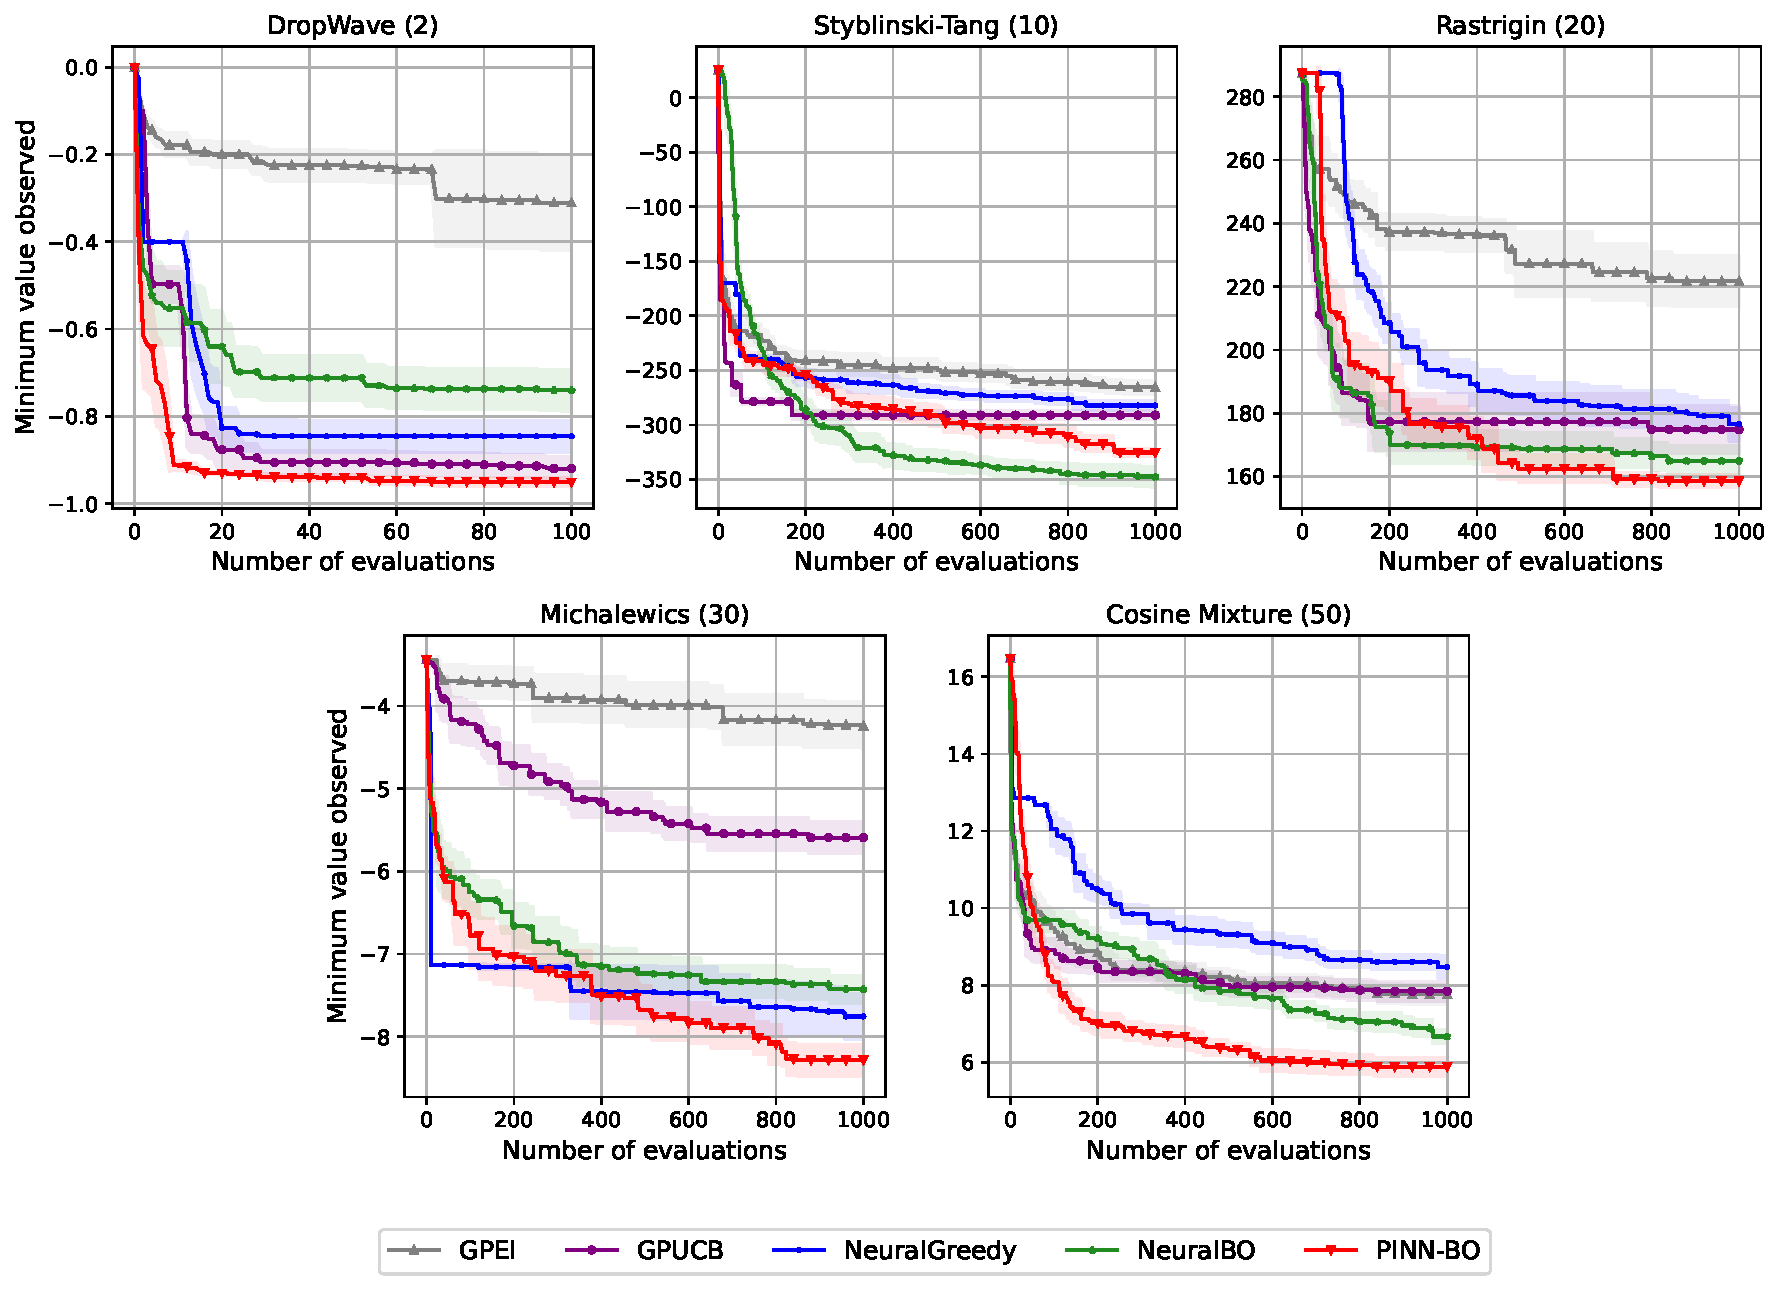
\includegraphics[width=\textwidth]{Figures/PINN-BO/pinn-bo_all_synthetic.pdf} 
  \caption{The optimization results for Rastrigin, Michalewics and Cosine Mixture, DropWave and Styblinski-Tang functions comparing the proposed PINN-BO with the baselines. The standard errors are shown by color shading.}
  \label{fig:pinn-bo_synthetic}
\end{figure}


\subsection{Real-world Applications}
In this section, we explore two real-world applications where the objective functions are constrained by specific \acp{pde}. We consider two tasks: (1) optimizing the Steady-State temperature distribution, satisfying the  Laplace equation, and (2) optimizing the displacement of a beam element, adhering to the non-uniform Euler-Bernoulli equation. We continue to compare our proposed method with the baselines mentioned in Section \ref{section:baselines}. 

\subsubsection{Optimizing Steady-State Temperature}
\label{section:pinn-bo_experiments_2d_laplace}
In this study, we showcase the benchmark optimization outcomes achieved by our proposed PINN-BO algorithm, comparing them with baseline methods for the steady-state temperature optimization task. The steady-state heat equation represents a special case of the heat equation when the temperature distribution no longer changes over time. It describes the equilibrium state of a system where the temperature is constant, and no heat is being added or removed.  The governing PDE for the temperature distribution is expressed as: $\nabla^2 T(x, y) = 0$, where $x, y$ are spatial variables that represent the positions within a two-dimensional space. We explore the heat equation in a domain where $x$ and $y$ lie within the defined range of $[0,2\pi]$. To thoroughly investigate the problem, we consider three different heat equations, where the solution of each problem is associated with one (unknown) boundary condition, each contributing to a deeper understanding of the system: 

 \paragraph{Heat Equation with Boundary Conditions 1}
 \label{para:heat1}
 \begin{align*}
     T(x, 0) &= 5\sin(y) + \sqrt{1+y} \\
    T(x, 2\pi) &= y\sin\left(3\cos(y) + 2\exp(y)\sin(y)\right) \\
   T(0, y) &= 10\cos(x) + x\exp(\sqrt{x^2 + \sin(x)}) \\
   T(2\pi, y) &= 3\sqrt{\exp(x\exp(-x))}\sin(x) + \cos(3x)\cos(3x)
 \end{align*}
 \paragraph{Heat Equation with Boundary Conditions 2}
 \label{para:heat2}
\begin{align*}
    T(x, 0) &= \sin(x) \cos(2x) + x^2\sqrt{3x}  + e^{\sin(x)} \\
    T(x, 2\pi) &= e^{\sin(x)} \sqrt{3x} + x^2 \cos(x)  \sin^2(x)   + e^{\cos(x)} \\
    T(0, y) &= \sqrt{2y}  \sin(y) + y^3\cos(2y)   + e^{\cos(y)} \\
    T(2\pi, y) &= \sin(y) \cos(2y) + y^3\sqrt{2y}   + e^{\sin(y)}
\end{align*}
\paragraph{Heat Equation with Boundary Conditions 3}
\label{para:heat3}
\begin{align*}
    T(x, 0) &= \left(\sin(x) + \cos(2x) \right) \sqrt{3x} + x^2 + e^{\sin(x)} \\
    T(x, 2\pi) &= \left(e^{\sin(x)} + \sqrt{3x} \right) \cos(x) + \left(\sin^2(x) + x^2\right)  e^{\cos(x)}
    \\
    T(0, y) &= \left(\sqrt{2y} + \sin(y)\right)  \left(\cos(2y) + y^3 \right) + e^{\cos(y)}\\
    T(2\pi, y) &= \left(\sin(y) + \cos(2y)\right) \left(\sqrt{2y} + y^3\right) + e^{\sin(y)}
\end{align*}
We utilized \texttt{py-pde}, a Python package designed for solving partial differential equations (PDEs), available at the following GitHub repository: \url{https://github.com/zwicker-group/py-pde}. This tool enabled us to obtain solutions to heat equations at various input points, with specific boundary conditions serving as the input data. In Figure \ref{fig:heat_dist}, the temperature distribution within the defined domain $[0, 2\pi]$ is visualized. It is important to emphasize that the boundary conditions used for benchmarking purposes are unknown to the methods employed. Adhering to the framework of black-box optimization, we assume that solving the PDEs incurs a substantial computational cost. The figure illustrates the spatial distribution of temperature values $T(x,y)$ across domain $[0, 2\pi] \times [0, 2\pi]$, with each subfigure corresponding to one of the mentioned boundary conditions.  
\begin{figure}[ht]
    \centering
    \begin{subfigure}[b]{0.49\textwidth}
        \centering
        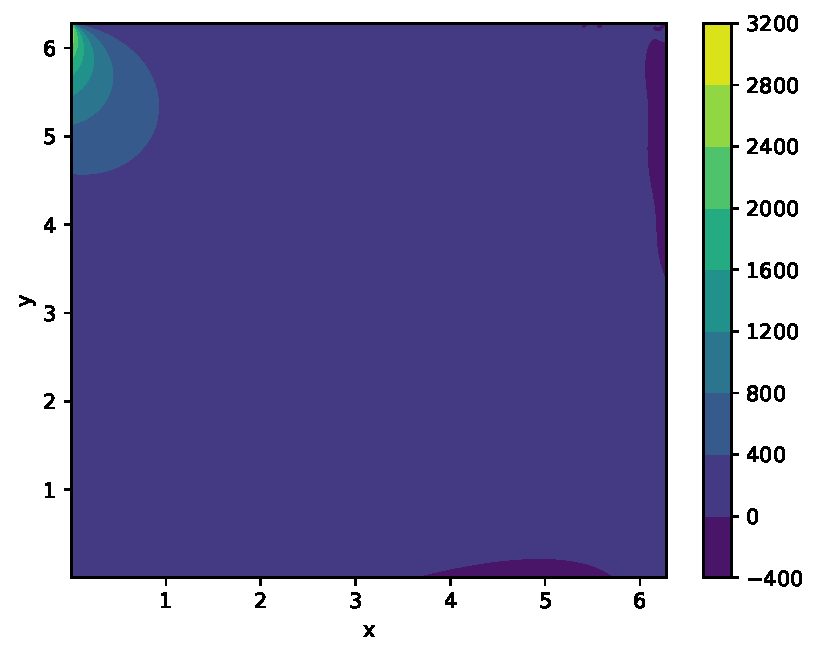
\includegraphics[width=\textwidth]{Figures/PINN-BO/heat_py_pde_1000_test_1.pdf}
        \caption{Solution of Temperature Equation with boundary conditions 1}
 \label{fig:heat_1_dist}
    \end{subfigure}
    \hfill
    \begin{subfigure}[b]{0.49\textwidth}
        \centering
        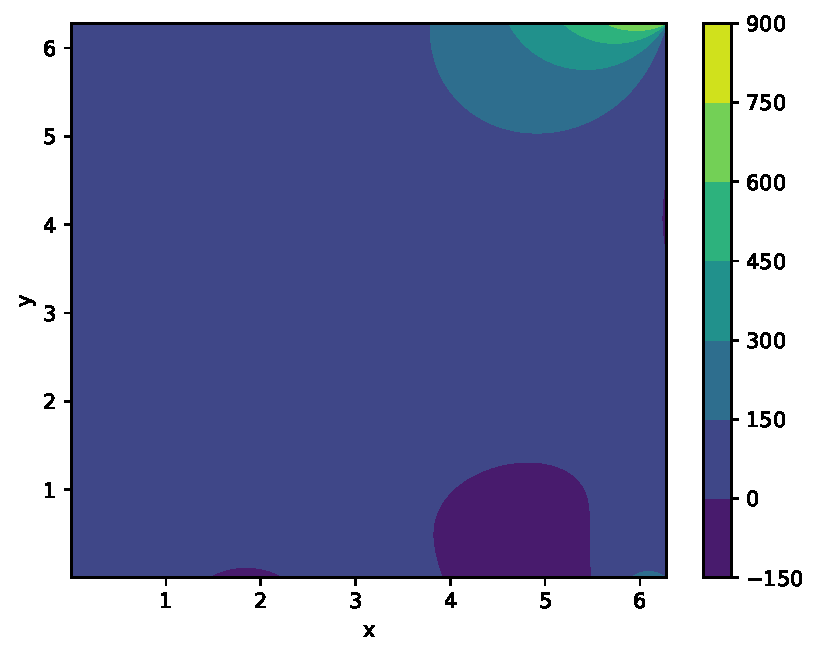
\includegraphics[width=1\textwidth]{Figures/PINN-BO/heat_py_pde_1000_test_2.pdf}
        \caption{Solution of Temperature Equation with boundary conditions 2}
        \label{fig:heat_2_dist}
    \end{subfigure}
    \hfill
    \begin{subfigure}[b]{0.5\textwidth}
        \centering
        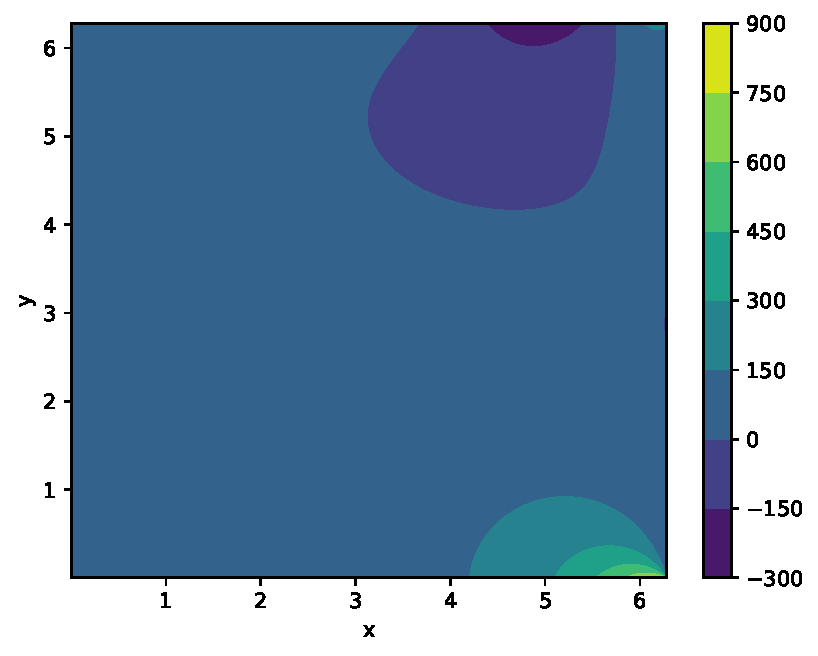
\includegraphics[width=\textwidth]{Figures/PINN-BO/heat_py_pde_1000_test_3.pdf}
        \caption{Solution of Temperature Equation with boundary conditions 3}
        \label{fig:heat_3_dist}
    \end{subfigure}
    \caption{The figures depict the solutions for temperature distributions governed by the heat equation, with each figure corresponding to a specific tuple of boundary conditions described in Section \ref{section:pinn-bo_experiments_2d_laplace}. It is evident that the region with the highest temperature is relatively small in comparison to the entire domain.}
    \label{fig:heat_dist}
\end{figure}

We conducted temperature optimization by identifying the locations $(x,y)$ where the temperature reaches its maximum. As illustrated in Figure \ref{fig:heat_dist}, the area with high temperatures is relatively small in comparison to the regions with medium or low temperatures. For each baseline, we performed the optimization process 10 times, computing the average results. The comparative outcomes are presented in Figure \ref{fig:heat_opt}. 
\begin{figure}[ht]
    \centering
    \begin{subfigure}[b]{0.49\textwidth}
        \centering
    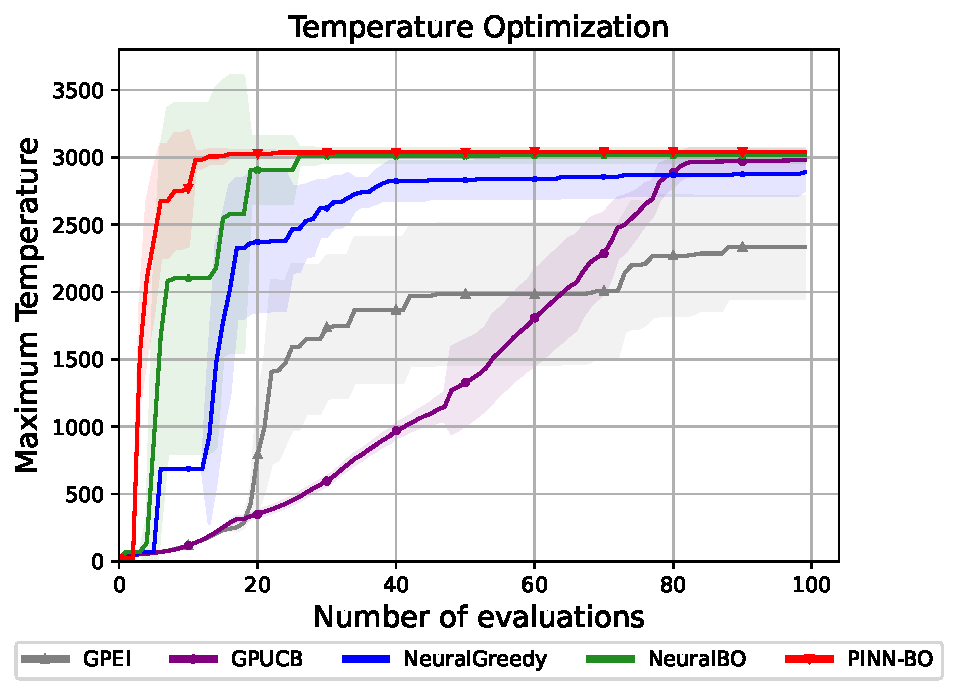
\includegraphics[width=\textwidth]{Figures/PINN-BO/Heat_dim_2_bc1.pdf}
        \caption{Temperature Optimization in case of boundary conditions 1}
 \label{fig:heat_1_opt}
    \end{subfigure}
    \hfill
    \begin{subfigure}[b]{0.49\textwidth}
        \centering
        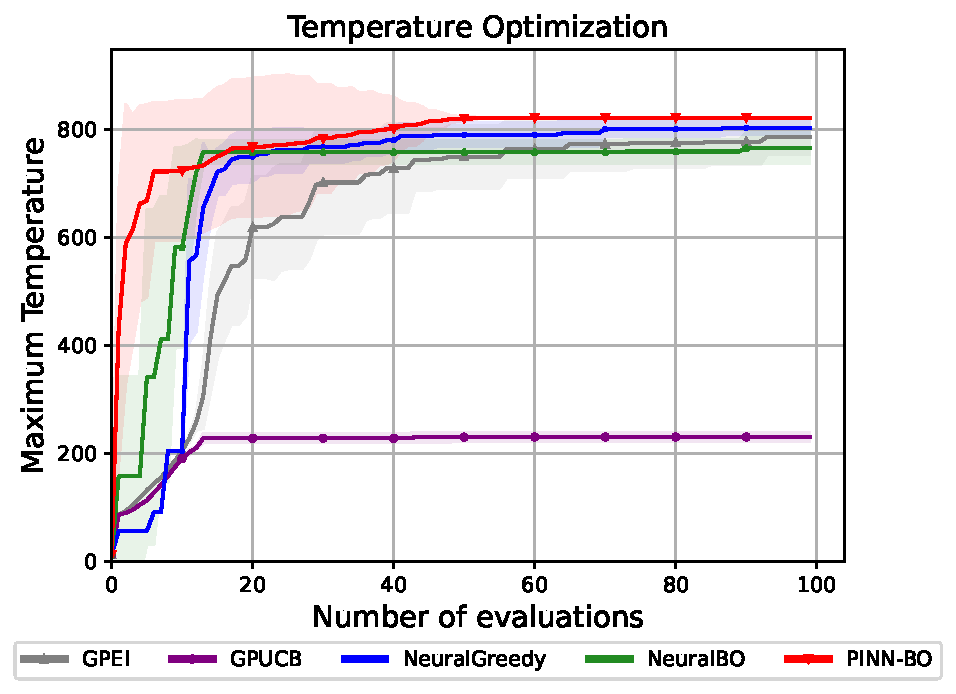
\includegraphics[width=1\textwidth]{Figures/PINN-BO/Heat_dim_2_bc2.pdf}
        \caption{Temperature Optimization in case of boundary conditions 2}
        \label{fig:heat_2_opt}
    \end{subfigure}
    \hfill
    \begin{subfigure}[b]{0.5\textwidth}
        \centering
        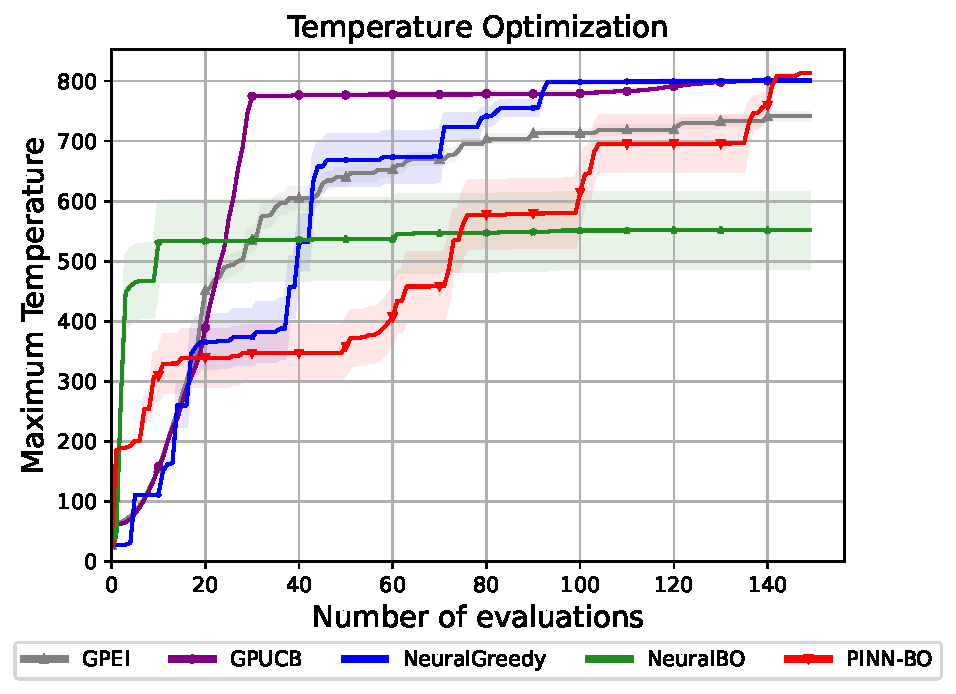
\includegraphics[width=\textwidth]{Figures/PINN-BO/Heat_dim_2_bc3.pdf}
        \caption{Temperature Optimization in case of boundary conditions 3}
        \label{fig:heat_3_opt}
    \end{subfigure}
    \caption{The figure shows the temperature optimization results of our PINN-BO and other baselines. For all three cases with different positions of maximum temperature, our PINN-BO performs better than all other baselines.}
    \label{fig:heat_opt}
\end{figure}


\subsubsection{Optimizing Beam Displacement}
We present the benchmark optimization outcomes obtained through our proposed method, PINN-BO, and the baseline approaches, addressing the task of minimizing the deflection of a non-uniform Euler-Bernoulli beam. The governing differential equation describing the behavior of a non-uniform Euler-Bernoulli beam is provided below: 
\begin{equation*}
    \frac{d^2}{dx^2} \left( EI(x) \frac{d^2 w(x)}{dx^2} \right) = q(x),
\end{equation*}
where
$EI(x)$ represents the flexural rigidity of the beam, which can vary with position $x$, and $w(x)$ represents the vertical displacement of the beam at position $x$ and 
$q(x)$ represents the distributed or concentrated load applied to the beam. 
In our implementation, we consider the detailed expression of $\text{EI}(x)$ and $q(x)$ as follows:
\begin{align*}
    \text{EI}(x) &= \frac{e^x}{\rho(x)},\\
    \rho(x) &= 2.4 x - 64 \pi^{2} e^{4 x} \sin{\left(4 \pi e^{2 x} \right)} - 396 e^{2 x} \sin{\left(20 x \right)} \\
    &+ 80 e^{2 x} \cos{\left(20 x \right)} + 16 \pi e^{2 x} \cos{\left(4 \pi e^{2 x} \right)} + 0.4
\end{align*}
We employed the Finite Difference Method (FDM) to solve the non-uniform Euler-Bernoulli beam equation. It's crucial to note that this step is solely for generating observations at each input point. Despite obtaining this solution, our methods and all baseline techniques continue to treat this solution as a black-box function, accessing observations solely through querying. In Figure \ref{fig:beam_illustration}, the displacement values $w(x)$ for $x \in (0,1)$ are illustrated. The optimization results for both our PINN-BO and the other baseline methods are presented in Figure \ref{fig:beam_opt}.
\clearpage
\begin{figure}[!t]
    \centering
    \begin{subfigure}[t]{0.44\textwidth}
        \centering
    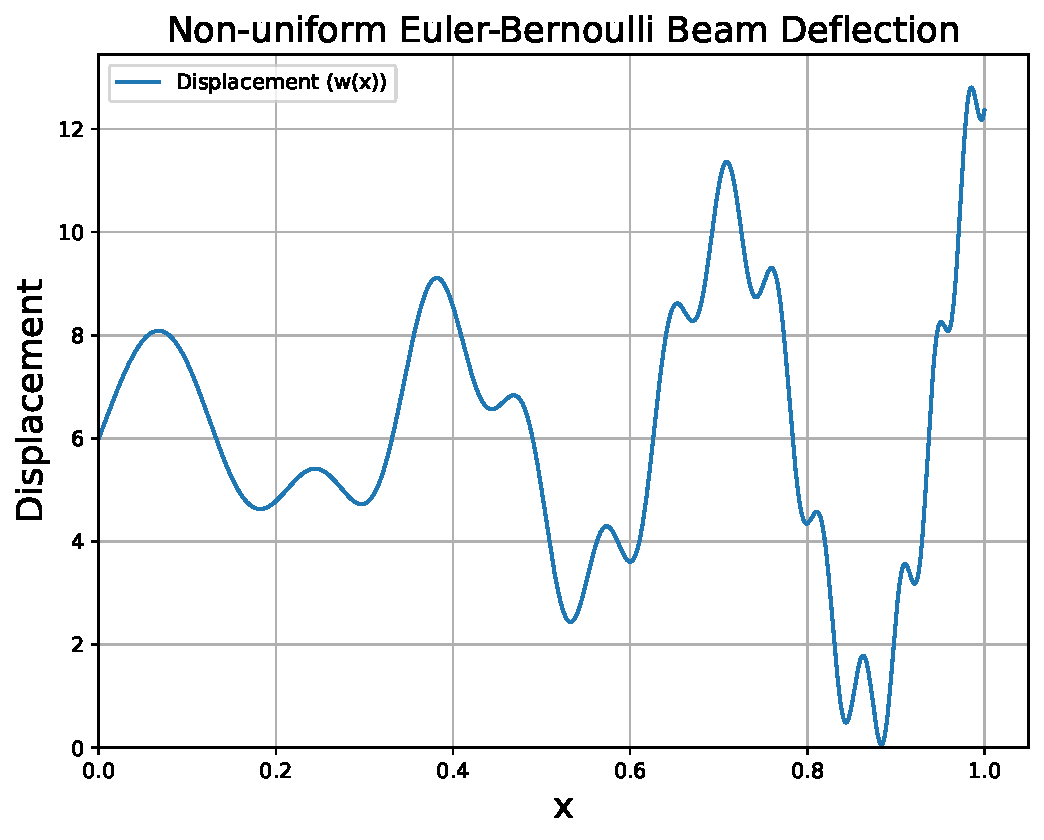
\includegraphics[width=\textwidth]{Figures/PINN-BO/beam.pdf}
    \caption{Displacement of non-uniform Euler beam}
     \label{fig:beam_illustration}
    \end{subfigure}
    \hfill
    \begin{subfigure}[t]{0.49\textwidth}
        \centering
        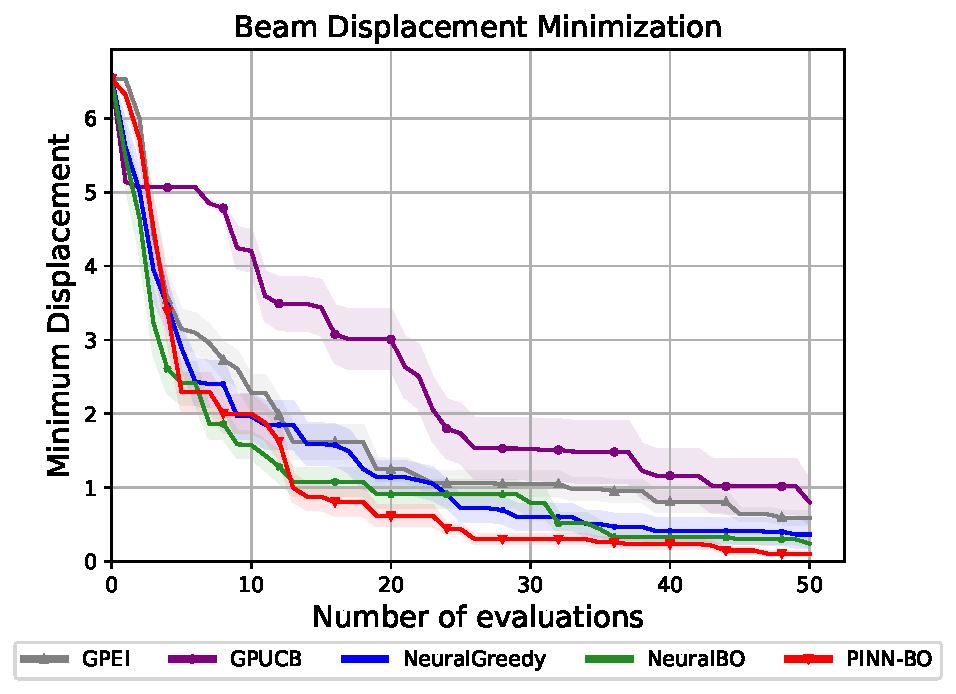
\includegraphics[width=1\textwidth]{Figures/PINN-BO/BeamDeflection_dim_1.pdf}
        \caption{Displacement Optimization of non-uniform Euler beam}
        \label{fig:beam_opt}
    \end{subfigure}
    \caption{Displacement of a non-uniform Euler Beam and minimum displacement found by our PINN-BO and the other baselines. The left panel illustrates the natural displacement profile of the non-uniform Euler beam under given loads $q(x)$,  flexural rigidity $EI(x)$, and boundary conditions. The right panel depicts the optimized position on the beam where the displacement is minimized, highlighting the location where the structural response is at its lowest.}
    \label{fig:beam}
\end{figure}



%  The steady-state heat equation is given by: $\nabla^2 T(x, y) = 0$, 
%  In this paper, our task is to find the best position $(x,y)$ that maximizes temperature $T$ within the defined domain. Formally, this problem can be defined as: 
% \begin{equation*}
%         \underset{x,y \in \mathcal{U}}{\max}  \;T(x,y) \text{ s.t. }  \nabla^2 T(x, y) = 0,
% \end{equation*}
% The details and the results of optimizing these heat equation problems are provided in Section A.2. The optimization results of our PINN-BO, in comparison to other baseline methods, for the first case of the heat equation, are depicted in Figure \ref{fig:heat_main}.

% \begin{figure}
%   \centering
%   \begin{subfigure}[t]{0.48\textwidth}
%     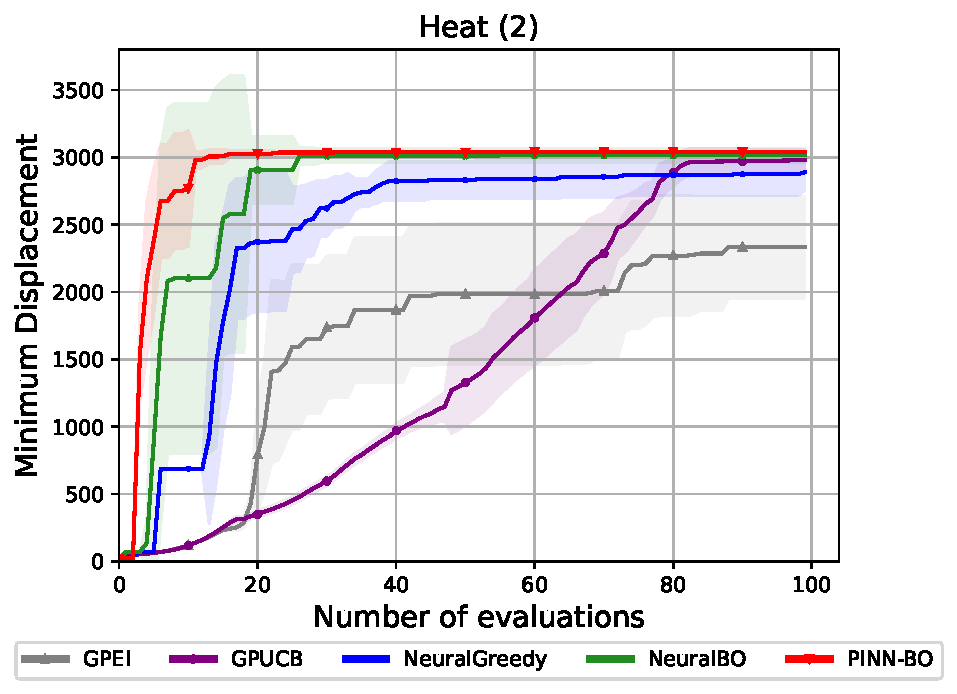
\includegraphics[width=\textwidth]{Figures/PINN-BO/Heat_dim_2.pdf}
%   \caption{The optimization results for finding the maximum temperature comparing the proposed PINN-BO with the baselines. It can be seen that, using the \ac{pde} heat equation, PINN-BO found the maximum temperature faster than all baselines.}
%   \label{fig:heat_main}
%   \end{subfigure}
%   \hfill
%   \begin{subfigure}[t]{0.48\textwidth}
%     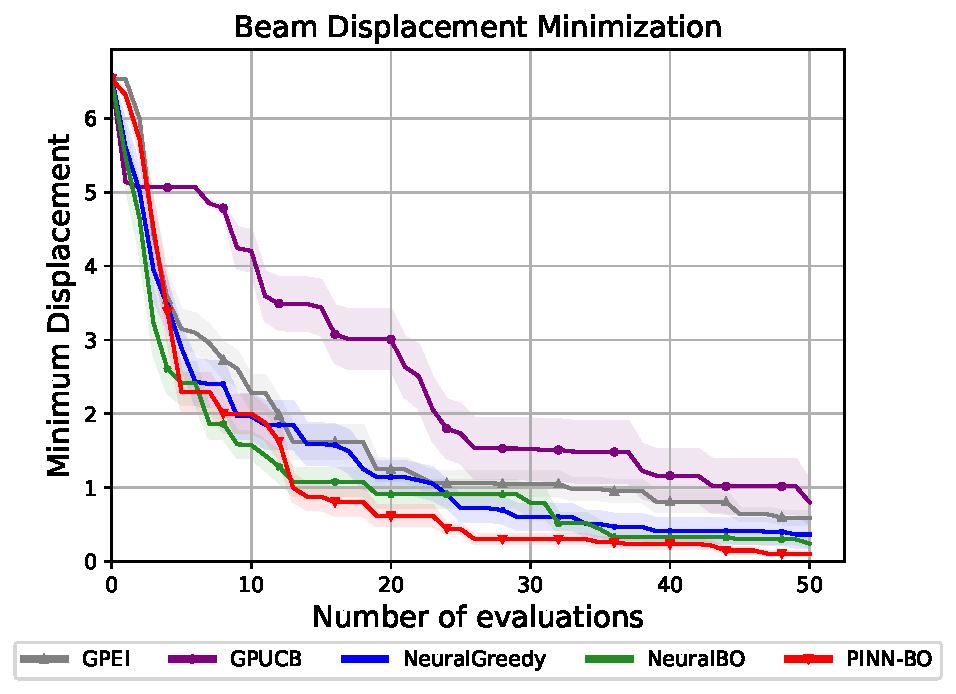
\includegraphics[width=\textwidth]{Figures/PINN-BO/BeamDeflection_dim_1.pdf}
%   \caption{The minimum displacement on the non-uniform Euler beam under given loads $q(x)$,  flexural rigidity $EI(x)$, and boundary conditions. In comparison with other baselines, our proposed PINN-BO found the location with the smallest displacement, ensuring stability when placing the load over the beam.}
%   \label{fig:beam_main}
%   \end{subfigure}
%   \caption{The optimization results for real-world applications comparing the proposed PINN-BO with the baselines.}
% \end{figure}

% \subsubsection{Optimizing Beam Displacement}
% Euler-Bernoulli beam theory is a widely used model in engineering and physics to describe the behavior of slender beams under various loads. The governing differential equation for a non-uniform Euler-Bernoulli beam is given by: 
% \begin{equation*}
%     \frac{d^2}{dx^2} \left( EI(x) \frac{d^2 w(x)}{dx^2} \right) = q(x),
% \end{equation*}
% where
% $EI(x)$ represents the flexural rigidity of the beam, which can vary with position $x$, and $w(x)$ represents the vertical displacement of the beam at position $x$, and $q(x)$ represents the distributed or concentrated load applied to the beam. The lower value deflection leads to a stiffer and more resilient structure, hence reducing the risk of structural failure and serviceability issues.  In this paper, we consider the task of finding the position $x$ that minimizes displacement $w(x)$. This problem can be defined as: 
% \begin{align*}
%     \underset{x \in \mathcal{S}}{\min}  \;
%         w(x) \\
% \text{ s.t. }  \frac{d^2}{dx^2} \left( EI(x) \frac{d^2 w(x)}{dx^2} \right) = q(x)
% \end{align*}


% \section{Conclusion}
% \label{section:pinn-bo_conclusion}
% We introduced a novel black-box optimization scenario incorporating \acfp{pde} as additional information. Our solution, PINN-BO, is a new algorithm tailored to this challenge. We conducted a theoretical analysis, demonstrating its convergence with a tighter regret bound. Through experiments involving synthetic benchmark functions and real-world optimization tasks, we validated the efficacy of our approach. Our method, due to using a neural network, is applicable to a broad set of optimization problems where the input space is complex (e.g. drug discovery), and can significantly accelerate the optimization by leveraging the auxiliary knowledge via \acp{pde}.  

\chapter{Conclusion} % Main chapter title

\label{chap:conclusion} % For referencing the chapter elsewhere, use \ref{chap:background}

In this thesis, we have introduced three methods that apply \acp{dnn} as an alternative to \acp{gp} for the surrogate models in \ac{bo}. We also extended the use of \ac{dnn} to different settings of \ac{bo}. These methods improved the scalability drawback of \ac{bo} with \ac{gp} while ensuring the optimization convergence. Further, \acp{dnn}-based \acl{bo} shows the potential application to high-dimensional structural data. We summarize our
contributions below and outline some potential future work in this area. 

\section{Contributions}
To address the computational costs and scalability limitations (particularly for structural inputs such as images or text, which are often accompanied by high-dimensional data), caused by the cubic complexity of kernel inversion in \acp{gp} used for \ac{bo}, this thesis focused on developing methods based on \acp{dnn} for both standard and extended \ac{bo} problems.

The key idea was first applied within the standard \ac{bo} setting. In \textbf{Chapter} \ref{chap:neural-bo}, a novel black-box optimization algorithm was introduced, where the unknown function was modeled using an over-parameterized \ac{dnn}. \ac{ntk} theory was employed to control network uncertainty, along with the \ac{ts} technique for selecting the next point for evaluation. Theoretical analysis of the algorithm's regret bound was demonstrated to show convergence and improved sample efficiency over existing methods. Additionally, the Neural-BO algorithm was shown to be scalable, with computational costs growing linearly with the number of data points, making it suitable for optimizing complex structured data like images and text. Experimental results on synthetic benchmarks and real-world optimization tasks confirmed that the algorithm outperformed current state-of-the-art methods in \ac{bo}. 

In \textbf{Chapter} \ref{chap:neural-cbo}, the \ac{dnn}-based approach was extended to address \ac{bo} with unknown, expensive constraints. Neural-CBO was introduced, where both the objective function and constraints were modeled by \acp{dnn}. \ac{ei} was used as the acquisition function for the objective, while the feasible region was defined using Lower Confidence Bound (LCB) conditions. Theoretical analysis indicated that cumulative regret and constraint violations had upper bounds comparable to those of \ac{gp}-based methods, under a more relaxed condition on network width. Experimental verification, conducted on synthetic and real-world tasks, demonstrated that Neural-CBO performed competitively with recent state-of-the-art approaches. 

In \textbf{Chapter} \ref{chap:pinn-bo}, a novel problem setting for \ac{bo} was introduced, integrating physical prior knowledge about the underlying black-box function through \acp{pde}, using \acp{pinn}. The PINN-BO algorithm enhanced sample efficiency by efficiently handling a broad class of \acp{pde}, thereby promoting the use of physical knowledge in \ac{bo}. It was ultimately demonstrated that this approach significantly improved practical performance when compared to existing methods across various synthetic and real-world benchmark functions.
 
\section{Future Directions}
In this thesis, the convergence of \ac{dnn}-based \ac{bo} approaches is demonstrated in terms of the maximum information gain, denoted as $\gamma_T$, with respect to the \ac{ntk}. As established by \citet{kassraie2022neural}, $\gamma_T$ is bounded by $\mathcal{O}(T^{1-d^{-1}})$, where $T$ represents the number of observations and $d$ the input dimensionality. In \textbf{Chapter} \ref{chap:neural-bo}, this result was utilized to prove that the Neural-BO algorithm achieves a sub-linear regret bound, which is crucial for ensuring efficient optimization. This result is based on the assumption that the observation noise is independent of the observed values. However, in more complex scenarios where the noise depends on prior observations, deriving a sublinear regret bound remains an open problem, suggesting an interesting avenue for future research, either by improving the upper bound of $\gamma_T$ or by designing a more refined algorithm to ensure sublinear convergence.

A related and equally promising direction for future work is the improvement of the theoretical analysis of PINN-BO, as discussed in \textbf{Chapter} \ref{chap:pinn-bo}. The current regret bound for this algorithm includes the interaction information value, which is influenced by the \ac{pde} observations, making the regret bound dependent on the specific \ac{pde}. While it has been shown that PINN-BO is capable of handling a broad class of \ac{pde} constraints, establishing a regret bound for each specific \ac{pde} class, such as linear \acp{pde}, remains a significant challenge. In Section \ref{section:pinn-bo_theoretical_analysis}, a regret bound is provided for a simple class of \acp{pde}, yet extending this analysis to more complex classes could significantly improve the understanding of how physical information, expressed through \acp{pde}, positively influences the optimization process. By analyzing the regret bound for each \ac{pde} class, the integration of physical knowledge into \acl{bo} can be deepened, thereby enhancing the efficiency and practicality of algorithms like PINN-BO. This approach would not only strengthen the theoretical foundations of PINN-BO but also broaden its application to real-world optimization problems governed by diverse physical laws.      



%----------------------------------------------------------------------------------------
%	THESIS CONTENT - APPENDICES
%----------------------------------------------------------------------------------------

\appendix % Cue to tell LaTeX that the following "chapters" are Appendices

% Include the appendices of the thesis as separate files from the Appendices folder
% Uncomment the lines as you write the Appendices

\chapter{Supplementary Material of Chapter \ref{chap:neural-bo}} 
\label{section:neural-bo_supp}

\section{Proof of Theoretical Analysis in Chapter \ref{chap:neural-bo}}
\label{section:neural-bo_appendix}
In this part, we provide the proof for Theorem \ref{theorem:neural-bo_main}. The main lemmas are from Lemma \ref{lemma:bound_hil} to Lemma \ref{lemma:min_sigma}. Some main lemmas require auxiliary lemmas to complete their proofs. These auxiliary lemmas are provided instantly after the main lemmas and later proved in Section \ref{section:neural-bo_aux_appendix}. 


To begin, we consider the following condition of the neural network width $m$
\begin{condition}
\label{cond:set}
The network width $m$ satisfies
  \begin{align*}
     m & \geq C \max \Big\{ \sqrt{\lambda} L^{-3/2} [\log (TL^2 \alpha)]^{3/2}, T^6 L^6 \log (TL/ \alpha) \max \{\lambda_0^{-4},1 \} ] \Big\} 
     \\
     m  & [\log m ]^{-3} \geq CTL^{12} \lambda^{-1} + CT^7 \lambda^{-8}L^{18}(\lambda + LT)^6 + CL^{21}T^7\lambda^{-7}(1 + \sqrt{T/ \lambda})^6,
    \end{align*} 
    where $C$ is a positive absolute constant.
\end{condition}
Under this flexible condition of the search space as mentioned in Section \ref{section:neural-bo_regret_analysis}, we need some new results. Following \citet{allen2019convergence}, we first define 
\begin{align*}
    \mathbf{h}_{i,0} = \mathbf{x}, \mathbf{h}_{i,l} = \phi(\mathbf{W}_l \mathbf{h}_{i, l-1}), l \in [L]
\end{align*}
as the output of the $l$-th hidden layer. With this definition, we provide a norm bound of $\mathbf{h}_{i, l-1}$ as follows.

\begin{lemma}[Lemma 7.1, \citep{allen2019convergence}]
\label{lemma:bound_hil}
If $\epsilon \in [0,1]$,  with probability at least $1-\mathcal{O}(nL)e^{-\Omega(m\epsilon^2/L)}$, we have
\[ \forall i \in [T], l \in [L], \norm{\mathbf{h}_{i, l-1}} \in [ae^{-\epsilon}, be^\epsilon] 
\]
\end{lemma}


The following lemma is the concentration property of sampling value $\widetilde{f}_t(\mathbf{x})$ from estimated mean value $h(\mathbf{x}; \boldsymbol{\theta}_{t-1})$.
\begin{lemma}
\label{lemma:sampling_bound}
For any $t \in [T]$, and any finite subset $\mathcal{D}_t \subset\ \mathcal{D}$,  pick $c_t =  \sqrt{4\log t + 2 \log \ \lvert \mathcal D_t \rvert}$. Then we have:  
\[\lvert \widetilde{f}_t(\mathbf{x}) - h(\mathbf{x}; \boldsymbol{\theta}_{t-1}) \rvert \leq c_t\nu_t \sigma_t(\mathbf{x}), \forall \mathbf{x} \in \mathcal{D}_t, \] 
holds with probability $\geq  1-t^{-2}$.
\end{lemma}

To prove Lemma \ref{lemma:sampling_bound}, we need a concentration bound on Gaussian distributions \citep{hoffman2013exploiting} as follows: 

\begin{sublemma}[\citep{hoffman2013exploiting}]
\label{lemma:neural-bo_gauss_concetration}
Consider a normally distributed random variable $X \sim \mathcal{N}(\mu, \sigma^2)$ and $\beta \geq 0$. The probability that $X$ is within a radius of $\beta \sigma$ from its mean can then be written as:
\[ \mathbb{P}(\lvert X - \mu\rvert \leq \beta  \sigma\ ) \geq 1-\exp(\beta^2/2)\]
\end{sublemma}
\begin{proof}[Proof of Lemma \ref{lemma:sampling_bound}]
Because the sampled value $\widetilde{f}_t(\mathbf{x})$ is sampled from  
\[
\mathcal{N}(h(\mathbf{x}; \boldsymbol{\theta}_{t-1}), \nu_t^2\sigma_t^2(\mathbf{x})),
\] 
applying the concentration property in Lemma \ref{lemma:neural-bo_gauss_concetration}, we have:

\[\mathbb{P}(\rvert \widetilde{f}_t(\mathbf{x}) -h(\mathbf{x}; \boldsymbol{\theta}_{t-1}) \lvert \leq c_t \nu_t \sigma_t(\mathbf{x}) \lvert \mathcal{F}_{t-1}) \geq 1-\exp(-c_t^2/2)
\]
Taking union bound over $\mathcal{D}_t$, we have for any $t$:
\[\mathbb{P}(\rvert \widetilde{f}_t(\mathbf{x}) - h(\mathbf{x}; \boldsymbol{\theta}_{t-1}) \lvert \leq c_t \nu_t \sigma_t(\mathbf{x}) \lvert \mathcal{F}_{t-1}) \geq 1-\rvert \mathcal{D}_t \rvert\exp(-c_t^2/2) \]
Picking $c_t = \sqrt{4 \log t + 2 \log \lvert \mathcal{D}_t \rvert}$, we get the bound:

 \begin{align*}
     \mathbb{P}(\rvert \widetilde{f}_t(\mathbf{x}) - h(\mathbf{x}; \boldsymbol{\theta}_{t-1}) \lvert \leq c_t \nu_t \sigma_t(\mathbf{x}) \lvert \mathcal{F}_{t-1}) \geq 1-\frac{1}{t^2}
 \end{align*}
\end{proof}

By combining Lemma \ref{lemma:bound_hil} with techniques used in Lemma 4.1 of \citet{cao2019generalization}, Lemma B.3 
 of \citet{cao2019generalization} and Theorem 5 
of \citet{allen2019convergence}, we achieve a concentration property of estimated value $h(\mathbf{x}; \boldsymbol{\theta}_{t-1})$ from its true value $f(\mathbf{x})$ as follows:
\begin{lemma}
\label{lemma:predictive_bound}
Suppose the width of the neural network $m$ satisfies Condition \ref{cond:set}. Given any $\alpha \in (0,1)$ and set $\eta = C(m\lambda + mLT)^{-1}$.  Then for any $t \in [T]$, we have

\[\lvert h(\mathbf{x}; \boldsymbol{\theta}_{t-1}) - f(\mathbf{x}) \rvert \leq \nu_t \sigma_t(\mathbf{x}) + \epsilon(m), \forall \mathbf{x} \in \mathcal{D}_t, \] holds with probability $\geq  1-\alpha/2$ and 
\begin{equation*}
    \begin{split}
     \epsilon(m) = & \frac{b}{a} C_{\epsilon,1} m^{-1/6}\lambda^{-2/3}L^3 \sqrt{\log m} + \frac{b}{a} C_{\epsilon,2} (1-\eta m\lambda)^J \sqrt{TL/\lambda}\\
     & + \left(\frac{b}{a}\right)^3 C_{\epsilon,3} m^{-1/6} \sqrt{\log m} L^4 T^{5/3} \lambda^{-5/3} (1+\sqrt{T/\lambda}), \\
    \end{split}
\end{equation*}
where $\{C_{\epsilon,i}\}_{i=1}^3$ are positive constants and $a,b$ is lower and upper norm bound of input $\mathbf{x}$ as assumed in Section \ref{section:neural-bo_problem_setting}.
\end{lemma}
First, we define some necessary notations about linear and kernelized models.  
\begin{definition}
\label{def:linear_kernelized_terms}
Let us define terms for the convenience as follows:
\begin{equation*}
\begin{split}
\mathbf{G}_t & = (\mathbf{g}(\mathbf{x}_1; \boldsymbol{\theta}_0),\cdots,\mathbf{g}(\mathbf{x}_t; \boldsymbol{\theta}_0))\\
     \mathbf{f}_t & = (f(\mathbf{x}_1), \cdots, f(\mathbf{x}_t))^\top \\
     \mathbf{y}_t & = (y_1, \cdots, y_t)^\top \\
     \boldsymbol{\epsilon}_t & = (f(\mathbf{x}_1) - y_1, \cdots, f(\mathbf{x}_t) - y_t)^\top,
\end{split}
\end{equation*}
\end{definition}
where $\boldsymbol{\epsilon}_t$ is the reward noise at time $t$. We recall that the definition of $\boldsymbol{\epsilon}_t$ is simply from our setting in Section \ref{section:neural-bo_problem_setting}. It can be verified that $\mathbf{U}_t = \lambda\mathbf{I} + \mathbf{G}_t\mathbf{G}_t^\top/m$. 
We also define $\mathbf{K}_t = \lambda\mathbf{I} + \mathbf{G}_t ^\top\mathbf{G}_t /m$. 
We next reuse a lemma from \citet{zhang2021neural} to bound the difference between the outputs of the neural network and the linearized model.

\begin{sublemma} 
\label{lemma:NN_vs_linear}
Suppose the network width $m$ satisfies Condition \ref{cond:set}.
Then, set $\eta = C_1(m\lambda + mLT)^{-1}$, with probability at least $1 - \alpha$ over the random initialization of $\boldsymbol{\theta}_0$, we have $\forall \mathbf{x} \in \mathcal{D}, 0 < a \leq \norm{\bf x}_2  \leq b$
\begin{equation*}
\begin{split}
    & \left \lvert h(\mathbf{x}; \boldsymbol{\theta}_{t-1})- \langle \mathbf{g}(\mathbf{x}; \boldsymbol{\theta}_0); \mathbf{G}_{t-1}^\top \mathbf{U}^{-1}_{t-1} \mathbf{r}_{t-1}/m \rangle \right\rvert \\ 
    \leq &  \frac{b}{a} C_{\epsilon,1} t^{2/3}m^{-1/6} \lambda^{-2/3} L^3 \sqrt{\log m} + \frac{b}{a} C_{\epsilon,2}(1 - \eta m \lambda)^J \sqrt{tL/ \lambda}\\
    & + \left(\frac{b}{a} \right)^3 C_{\epsilon,3} m^{-1/6} \sqrt{\log m} L^4 t^{5/3} \lambda ^{-5/3} \left(1 + \sqrt{t/\lambda} \right),
\end{split}
\end{equation*}
where $\{C_{\epsilon,i}\}_{i=1}^3$ are positive constants. We provide the proof for this lemma in \ref{NN_vs_linear_proof}.
\end{sublemma}

\begin{sublemma}
\label{lemma:noise_affeted_bound}
Let $\alpha \in (0,1)$. Recall that matrix $\mathbf{U}_{t-1}$ is defined in Algorithm \ref{alg:Neural-BO}, $\mathbf{G}_{t-1}$ is defined in Definition \ref{def:linear_kernelized_terms} and $\mathcal{\epsilon}_{t-1}$ is i.i.d sub-Gaussian  observation noises up to optimization iteration $t-1$, with parameter $R$. Then with probability  $1-\alpha$, we have
\[ \left\lvert \mathbf{g}(\mathbf{x}; \boldsymbol{\theta}_0)^\top \mathbf{U}^{-1}_{t-1} \mathbf{G}_{t-1} \boldsymbol{\epsilon}_{t-1}/m   \right\rvert \leq \sigma_t(\mathbf{x})\frac{R}{\sqrt{\lambda}} \sqrt{2 \log(\frac{1}{\alpha})}\]
\end{sublemma}
The proof for Lemma \ref{lemma:noise_affeted_bound} is given in \ref{noise_affeted_bound_proof}. Then, the following lemma provides the upper bound for approximating the NTK with the empirical gram matrix of the neural network at initialization by the maximum information gain associated with the NTK. 

\begin{sublemma}
\label{lemma:log_det_Kt_bound}
Let $\alpha \in (0,1)$. If the network width $m$ satisfies  $m \geq C T^6L^6 \log(TL/\alpha)$, then with probability at least $1-\alpha$, with the points chosen from Algorithm \ref{alg:Neural-BO}, the following holds for every $t \in [T]$:
\[ \log \det (\mathbf{I} + \lambda^{-1} \mathbf{K}_t) \le 2\gamma_t + 1,\]
where $\gamma_t$ is maximum information gain associated with the kernel $k_\textup{NTK}$. We provided the proof of Lemma \ref{lemma:log_det_Kt_bound} in \ref{log_det_Kt_bound_proof}.
\end{sublemma}

\begin{sublemma}[Lemma D.2, \citep{kassraie2022neural}] 
\label{lemma:RKHS_expression}
Let $\alpha \in (0,1)$. Under Assumption \ref{assumption:sufficient_exploration} , if the network width $m$ satisfies  $m \geq C T^6L^6 \log(TL/\alpha)$ and $f$ be a member of $\mathcal{H}_{k_\text{NTK}}$ with bounded RKHS norm $\norm{f}_{k_\text{NTK}} \leq B$, then with probability at least $1-\alpha$, there exists $\mathbf{w} \in \mathbb{R}^p$ such that 
\[ f(\mathbf{x}) = \langle \mathbf{g}(\mathbf{x}; \boldsymbol{\theta}_0), \mathbf{w} \rangle, \norm{\mathbf{w}}_2 \leq \sqrt{\frac{2}{m}}B \]
\end{sublemma}
We remark that in our proofs, we assume $k_{\text{NTK}}(\mathbf{x}, \mathbf{x}) \leq 1$ for simplicity. Now we are going on to prove Lemma \ref{lemma:predictive_bound}
\begin{proof}[Proof of Lemma \ref{lemma:predictive_bound}]
First of all, since m satisfies Condition \ref{cond:set}, then with the choice of $\eta$, the condition required in Lemma \ref{lemma:NN_vs_linear} - \ref{lemma:log_det_Kt_bound} are satisfied. Thus, taking a union bound, we have with probability at least $1 - 3\alpha$, that the bounds provided by these lemmas hold. 
As we assume that $f$ is in RKHS $\mathcal{H}_{k_\textup{NTK}}$ with NTK kernel, and $\mathbf{g}(\mathbf{x}; \boldsymbol{\theta}_0)/\sqrt{m}$  can be considered as finite approximation of $\varphi(\cdot)$, the feature map of the NTK from $\mathbb{R}^d \rightarrow \mathcal{H}_{k_\textup{NTK}}$. From Lemma \ref{lemma:RKHS_expression} , there exists $\mathbf{w} \in \mathbb{R}^p$ such that $f(\mathbf{x}) = \langle \mathbf{g}(\mathbf{x}; \boldsymbol{\theta}_0), \mathbf{w} \rangle = \mathbf{g}(\mathbf{x}; \boldsymbol{\theta}_0)^\top \mathbf{w}$. 
Then for any $t \in [T]$, we will first provide the difference between the target function and the linear function
$\langle \mathbf{g}(\mathbf{x}; \boldsymbol{\theta}_0); \mathbf{U}^{-1}_{t-1} \mathbf{G}_{t-1} \mathbf{r}_{t-1}/m \rangle$ as:
\begin{equation}
\label{ieqn:confidence_interval}
    \begin{split}
         & \left \lvert f(\mathbf{x}) - \langle \mathbf{g}(\mathbf{x}; \boldsymbol{\theta}_0); \mathbf{U}^{-1}_{t-1} \mathbf{G}_{t-1} \mathbf{r}_{t-1}/m \rangle   \right \rvert  \\
        & = \left\lvert f(\mathbf{x}) - \mathbf{g}(\mathbf{x}; \boldsymbol{\theta}_0)^\top  \mathbf{U}^{-1}_{t-1} \mathbf{G}_{t-1} \mathbf{r}_{t-1}/m \right\rvert \\
        % & = \left\lvert f(\mathbf{x}) - \mathbf{g}(\mathbf{x}; \boldsymbol{\theta}_0)^\top \mathbf{U}^{-1}_{t-1} \mathbf{G}_{t-1} \mathbf{f}_{t-1}/m - \mathbf{g}(\mathbf{x}; \boldsymbol{\theta}_0)^\top \mathbf{U}^{-1}_{t-1} 
        % \mathbf{G}_{t-1}\boldsymbol{\epsilon}_{t-1}/m \right\rvert \\
        & \leq \left\lvert f(\mathbf{x}) - \mathbf{g}(\mathbf{x}; \boldsymbol{\theta}_0)^\top  \mathbf{U}^{-1}_{t-1}
        \mathbf{G}_{t-1}\mathbf{f}_{t-1}/m \right\rvert + 
        \left\lvert \mathbf{g}(\mathbf{x}; \boldsymbol{\theta}_0)^\top \mathbf{U}^{-1}_{t-1}
        \mathbf{G}_{t-1} \boldsymbol{\epsilon}_{t-1}/m \right\rvert\\
        & = \left\lvert \mathbf{g}(\mathbf{x}; \boldsymbol{\theta}_0)^\top \mathbf{w} - \mathbf{g}(\mathbf{x}; \boldsymbol{\theta}_0)^\top  \mathbf{U}^{-1}_{t-1} 
        \mathbf{G}_{t-1}
        \mathbf{G}_{t-1}^\top \mathbf{w}/m \rangle \right\rvert + 
        \left\rvert  \mathbf{g}(\mathbf{x}; \boldsymbol{\theta}_0)^\top \mathbf{U}^{-1}_{t-1} \mathbf{G}_{t-1} \boldsymbol{\epsilon}_{t-1}/m  \right\rvert\\
        & = \left\lvert \mathbf{g}(\mathbf{x}; \boldsymbol{\theta}_0)^\top \left( \mathbf{I} -  \mathbf{U}^{-1}_{t-1}  \mathbf{G}_{t-1} \mathbf{G}_{t-1}^\top/m  \right) \mathbf{w}  \right \vert + 
        \left\lvert  \mathbf{g}(\mathbf{x}; \boldsymbol{\theta}_0)^\top \mathbf{U}^{-1}_{t-1} \mathbf{G}_{t-1} \boldsymbol{\epsilon}_{t-1}/m  \right\rvert \\
        & = \left\lvert \mathbf{g}(\mathbf{x}; \boldsymbol{\theta}_0)^\top \left( \mathbf{I} -  \mathbf{U}^{-1}_{t-1} \left( \mathbf{U}_{t-1} -\lambda \mathbf{I} \right)  \right) \mathbf{w}  \right \vert +
        \left \lvert  \mathbf{g}(\mathbf{x}; \boldsymbol{\theta}_0)^\top \mathbf{U}^{-1}_{t-1} \mathbf{G}_{t-1} \boldsymbol{\epsilon}_{t-1}/m  \right \rvert \\
        & = \left\lvert \lambda \mathbf{g}(\mathbf{x}; \boldsymbol{\theta}_0)^\top \mathbf{U}^{-1}_{t-1} \mathbf{w}  \right\rvert  + \left\lvert \mathbf{g}(\mathbf{x}; \boldsymbol{\theta}_0)^\top \mathbf{U}^{-1}_{t-1} \mathbf{G}_{t-1} \boldsymbol{\epsilon}_{t-1}/m   \right\rvert \\
        & \leq \norm{\mathbf{w}}_{k_{\text{NTK}}}  \norm{ \lambda  \mathbf{U}^{-1}_{t-1} \mathbf{g}(\mathbf{x}; \boldsymbol{\theta}_0)}_{k_{\text{NTK}}} + \left\lvert \mathbf{g}(\mathbf{x}; \boldsymbol{\theta}_0)^\top \mathbf{U}^{-1}_{t-1} \mathbf{G}_{t-1} \boldsymbol{\epsilon}_{t-1}/m   \right\rvert \\
        & \leq  \norm{\mathbf{w}}_{k_{\text{NTK}}}  \sqrt {\lambda \mathbf{g}(\mathbf{x}; \boldsymbol{\theta}_0)^\top \mathbf{U}^{-1}_{t-1} \mathbf{g}(\mathbf{x}; \boldsymbol{\theta}_0)}  + \left\lvert \mathbf{g}(\mathbf{x}; \boldsymbol{\theta}_0)^\top \mathbf{U}^{-1}_{t-1} \mathbf{G}_{t-1} \boldsymbol{\epsilon}_{t-1}/m   \right\rvert \\
        & \leq \sqrt{2}B \sigma_t(\mathbf{x}) + \sigma_t(\mathbf{x})\frac{R}{\sqrt{\lambda}} \sqrt{2 \log(\frac{1}{\alpha})} \\
    \end{split}
\end{equation}
where the first inequality uses triangle inequality and the fact that $\mathbf{r}_{t-1}= \mathbf{f}_{t-1} + \boldsymbol{\epsilon}_{t-1}$. The second inequality is from the reproducing property of function relying on RKHS, and the fourth equality is from the verification noted in Definition  \ref{def:linear_kernelized_terms}. The last inequality directly uses the results from Lemma \ref{lemma:noise_affeted_bound} and Lemma \ref{lemma:RKHS_expression}. We have a more compact form of the inequality \ref{ieqn:confidence_interval} as: 
\[\rvert f(\mathbf{x}) - \langle \mathbf{g}(\mathbf{x}; \boldsymbol{\theta}_0); \mathbf{U}^{-1}_{t-1} \mathbf{G}_{t-1} \mathbf{r}_{t-1}/m \rangle \lvert \leq \nu_t \sigma_t (\mathbf{x}), 
\]
where we set $\nu_t = \sqrt{2}B + \frac{R}{\sqrt{\lambda}}\sqrt{2 \log(1/ \alpha)}$. 
Then, by combining this bound with
Lemma \ref{lemma:NN_vs_linear}, we have
% conclude that there exist positive constants $\Bar{C}_1,  \Bar{C}_2, \Bar{C}_3$ so that

\begin{equation*}
    \begin{split}
        \lvert h(\mathbf{x}; \boldsymbol{\theta}_{t-1}) - f(\mathbf{x}) \rvert & \leq \nu_t \sigma_t (\mathbf{x}) + \frac{b}{a} C_{\epsilon,1} t^{2/3}m^{-1/6} \lambda^{-2/3} L^3 \\ &
        \quad + \frac{b}{a} C_{\epsilon,2}(1 - \eta m \lambda)^J \sqrt{tL/\lambda} \\ &
        \quad +  \left(\frac{b}{a} \right)^3 C_{\epsilon,3} m^{-1/6} \sqrt{\log m} L^4 t^{5/3} \lambda ^{-5/3} \left(1 + \sqrt{t/\lambda}  \right) \\
        & \leq \nu_t \sigma_t (\mathbf{x}) + \epsilon(m)
    \end{split}
\end{equation*}
% where $\epsilon(m)$ is defined by adding all of the additional terms and taking $t = T$ 
% \begin{equation*}
%     \begin{split}
%      \epsilon(m) & = \Bar{C}_1 T^{2/3} m^{-1/6}\lambda^{-2/3}L^3 \sqrt{\log m} + \Bar{C}_2 (1-\eta\ m \lambda)^J \sqrt{TL/\lambda}\\
%      & + \Bar{C}_3 m^{-1/6} \sqrt{\log m} L^4 T^{5/3} \lambda^{-5/3} (1+\sqrt{T/\lambda}) \\
%     \end{split}
% \end{equation*}
% where is exactly the same form defined in \ref{lemma:predictive_bound}. 
By setting $\alpha $ to $\alpha/3$ (required by the union bound discussed at the beginning of the proof) and taking $t=T$, we get the result presented in Lemma \ref{lemma:predictive_bound}.
\end{proof}

The next lemma gives a lower bound of the probability that the sampled value $\widetilde{f}_t (\mathbf{x})$ is larger than the true function value up to the approximation error $\epsilon(m)$.
\begin{lemma}
\label{lemma:sampled_value_vs_real_value}
For any $t \in [T], \mathbf{x} \in D$, we have $\mathbb{P}(\widetilde{f}_t (\mathbf{x}) + \epsilon(m) > f(\mathbf{x})) \geq (4e\pi)^{-1}$.
\end{lemma}

\begin{proof}[Proof of Lemma \ref{lemma:sampled_value_vs_real_value}]
    Following proof style of Lemma 8 in \citet{zhou2020neural}, using Lemma \ref{lemma:predictive_bound} and Gaussian anti-concentration property, we have 
\begin{equation*}
    \begin{split}
        & \mathbb{P}(\widetilde{f_t}(\mathbf{x}) + \epsilon(m) > f(\mathbf{x}) \lvert \mathcal{F}_{t-1}) \\
        = & \mathbb{P} \Bigg(\frac{\widetilde{f_t}(\mathbf{x}) - h(\mathbf{x}; \boldsymbol{\theta}_{t-1}) }{\nu_t \sigma_t(\mathbf{x})} >   \frac{ \lvert f(\mathbf{x}) - h(\mathbf{x}; \boldsymbol{\theta}_{t-1}) \rvert - \epsilon(m) }{\nu_t \sigma_t(\mathbf{x})}  \Bigg \lvert \mathcal{F}_{t-1} \Bigg) \geq \frac{1}{4e\pi}
% \\
% \geq & \mathbb{P} \Bigg(\frac{\widetilde{f_t}(\mathbf{x}) - f(\mathbf{x};\boldsymbol{\theta}_{t-1})}{\nu_t \sigma_t(\mathbf{x})} >  1 \Bigg \lvert \mathcal{F}_{t-1} \Bigg) \geq \frac{1}{4e\pi}
    \end{split}
\end{equation*}
\end{proof}




For any step $t$, we consider how the standard deviation of the estimates for each point is, in comparison with the standard deviation for the optimal value.
Following \citet{zhang2021neural}, we divide the discretization $\mathcal D_t$ into two sets: saturated and unsaturated sets. For more details, we define the set of saturated points as:

\begin{equation}
\label{def:saturated_set}
S_t = \{\forall \mathbf{x} \in \mathcal{D}_t, f([\mathbf{x}^*]_t) - f(\mathbf{x}) \geq (1+c_t)\nu_t \sigma_t(\mathbf{x})+ 2\epsilon(m)\}
\end{equation}

% We define an event $\mathcal{E}^\sigma_t$ as follows

% $$\mathcal{E}^\sigma_t = \{ \forall \mathbf{x} \in \mathcal D_t, \rvert \widetilde{f_t} - f(\mathbf{x}; \boldsymbol{\theta}_{t-1}) \lvert \leq c_t \nu_t \sigma_t(\mathbf{x})  \},$$
% where $c_t = \sqrt{4 \log t  + 2 \log \lvert \mathcal D_t \rvert}$. Based on Lemma \ref{lemma:sampling_bound}, event $\mathcal{E}^\sigma_t$ holds w.p $1-t^{-2}$.

% We also define an event $\mathcal{E}^\mu_t$ as follows

% $$\mathcal{E}^\mu_t = \{\forall \mathbf{x} \in \mathcal D, \rvert f(\mathbf{x}; \boldsymbol{\theta}_{t-1}) - f(\mathbf{x}) \lvert \leq \nu_t \sigma_t + \epsilon(m) \}$$ 
% Event $\mathcal{E}^\mu_t$ holds w.p $1-\alpha/2, \alpha \in (0,1)$, from Lemma \ref{lemma:predictive_bound}.
The following lemma shows that, the algorithm can pick unsaturated points $\mathbf{x}_t$ with high probability. 
\begin{lemma}[Lemma 4.5, \citep{zhou2020neural}]
\label{lemma:unsaturated_points}

Let $\mathbf{x}_t$ be the chosen point at step $t \in [T]$. Then, $\mathbb{P}(\mathbf{x}_t \not\in S_t \lvert \mathcal{F}_{t-1}) \geq \frac{1}{4e\sqrt{\pi}} - \frac{1}{t^2}$
\end{lemma}

The next lemma bounds the expectation of instantaneous regret at each round conditioned on history $\mathcal{F}_{t-1}$.

\begin{lemma}
\label{lemma:neural-bo_regret_expectation}
Suppose the width of the neural network m satisfies Condition \ref{cond:set}. Set $\eta = C_1(m\lambda + mLT)^{-1}$. Then with probability at least $1- \alpha$, we have for all $t \in [T]$ that
\begin{equation*}
\mathbb{E}[f(\mathbf{x}^*) - f(\mathbf{x}_t) \lvert \mathcal{F}_{t-1}] \leq C_2 (1+c_t)\nu_t \sqrt{L} \mathbb{E}[ \min(\sigma_t(\mathbf{x}_t),B)\lvert\mathcal{F}_{t-1}] + 4\epsilon(m) + \frac{2B+1}{t^2}
\end{equation*}
where $C_1, C_2$ are absolute constants.
\end{lemma}

\begin{proof} [Proof of Lemma \ref{lemma:neural-bo_regret_expectation}]
     
This proof inherits the proof of Lemma 4.6 in \citet{zhang2021neural}, and by using the result of unsaturated point $\mathbf{x}_t$ in Lemma \ref{lemma:unsaturated_points}, along with $\lvert f(x)  \rvert = \lvert \langle f, k(x,\cdot) \rangle \rvert \leq B$ instead of $\lvert f(x) \rvert  \leq 1$ as in \citet{zhang2021neural}, we have the following result:
\begin{equation*}
\begin{split}
    &  \mathbb{E} [f([\mathbf{x}^*]_t) - f(\mathbf{x}_t) \mid \mathcal{F}_{t-1}] \\
    \leq  & 44e\sqrt{\pi}(1+c_t )\nu_t C_1\sqrt {L} \mathbb{E}[\min \{\sigma_t(\mathbf{x}_t),B\} \mid \mathcal{F}_{t-1}] + 4\epsilon(m) + \frac{2B}{t^2}
\end{split}
\end{equation*}
Now using Eqn \ref{eqn:rkhs_lipschitz}, we have the instantaneous regret at round $t$
\[
r_t = f(\mathbf{x}^*) - f([\mathbf{x}^*]_t) + f([\mathbf{x}^*]_t) - f(\mathbf{x}_t) \leq \frac{1}{t^2} + f([\mathbf{x}^*]_t) - f(\mathbf{x}_t)
\]
Taking conditional expectation, we have the result as stated in Lemma \ref{lemma:neural-bo_regret_expectation}.

\end{proof}

The next lemma bounds the cumulative regret $\sum_{t=1}^T r_t$ after $T$ iterations. 
\begin{lemma}
\label{lemma:neural-bo_regret_bound}
Suppose the width of the neural network m satisfies Condition \ref{cond:set}. Then set $\eta = C_1(m\lambda + mLT))^{-1}$, we have, with probability at least $1-\alpha$, that
\begin{equation*}
\begin{split}
   \sum_{t=1}^T f(\mathbf{x^*}) - f(\mathbf{x}_t)
    & \leq  4T \epsilon(m) + \frac{(2B+1)\pi^2}{6} + C_2(1+c_T)\nu_t \sum^T_{t=1} \min(\sigma_t(\mathbf{x}_t),B) \\ &
    + (4B+ C_3 (1+c_T)\nu_t L + 4\epsilon(m)) \sqrt{2 \log(1/\alpha)T}
\end{split}
\end{equation*}
where $C_1, C_2, C_3$ are absolute constants.
\end{lemma}
\begin{proof}[Proof of Lemma \ref{lemma:neural-bo_regret_bound}]
    

Similar to Lemma \ref{lemma:neural-bo_regret_expectation}, we utilize the proof of Lemma 4.7 in \citet{zhang2021neural} or equivalent proof of Lemma 13 in \citet{chowdhury2017kernelized}. Then with $f(\mathbf{x})\leq B$, we have

\begin{equation*}
\begin{split}
    \sum_{i=1}^T r_t & \leq 4T\epsilon(m) + (2B+1) \sum_{i=1}^T t^{-2} + C_1 (1+c_T)\nu_t\sum_{i=1}^T \min(\sigma_t(\mathbf{x}_t),B) \\ & + (4B + C_1C_2(1 + c_T )\nu_t L + 4\epsilon(m))\sqrt{2 \log(1/\alpha)T}
\end{split} 
\end{equation*}
\end{proof}
The next lemma gives a bound on the sum of variance $\sum_{i=1}^T \min(\sigma_t(\mathbf{x}_t), B)$ which appears in Lemma \ref{lemma:neural-bo_regret_bound}.
\begin{lemma}
\label{lemma:min_sigma}
Suppose the width of the neural network m satisfies Condition \ref{cond:set}. Then set $\eta = C_1(m\lambda + mLT))^{-1}$, we have, with probability at least $1-\alpha$, that
\begin{equation*}
    \sum_{i=1}^T \min(\sigma_t(\mathbf{x}_t),B) \leq \sqrt{\frac{\lambda BT}{\log(B+1)} (2\gamma_T+1) } 
\end{equation*}
% where $\gamma_T$ is the maximum information gain of the exact NTK.
\end{lemma}
To prove lemma \ref{lemma:min_sigma}, we first need to utilize a technical lemma:
\begin{sublemma}
\label{lemma:min_B_vs_cov_norm}
Let $\{ \mathbf{v}_t\}_{t=1}^\infty$ be a sequence in $\mathbb{R}^p$, and
define $\mathbf{V}_t = \lambda \mathbf{I} + \sum^t_{i=1} \mathbf{v}_i\mathbf{v}_i^\top$ and $B$ is a positive constant. If $\lambda \geq 1$, then

\[ 
\sum_{i=1}^T \min \{ \mathbf{v}_t^\top \mathbf{V}_{t-1}^{-1}\mathbf{v}_{t-1}, B\} \leq \frac{B}{\log(B+1)} \log \det(\mathbf{I} + \lambda^{-1}\sum_{i=1}^T \mathbf{v}_i\mathbf{v}_i^\top)
\]
\end{sublemma}
\ref{min_B_vs_cov_norm_proof} provided the proof for Lemma \ref{lemma:min_B_vs_cov_norm}. Now, we start to prove Lemma \ref{lemma:min_sigma}
\begin{proof}[Proof of Lemma \ref{lemma:min_sigma}]

From Cauchy-Schwartz inequality, we have 
\begin{equation*}
    \begin{split}
        \sum_{i=1}^T \min \{\sigma_t(\mathbf{x}_t), B\} & \leq \sqrt{T \sum_{i=1}^T \min \{\sigma_t^2(\mathbf{x}_t), B\}} \\
        % \sum_{i=1}^T \min \{\Bar{\sigma}_t(\mathbf{x}_t), B\} + \sum_{i=1}^T \sigma_t - \Bar{\sigma}_t
        % \\
        % & + C_1 T^{13/6} \sqrt{\log m}  m^{-1/6} \lambda^{-2/3} L^{9/2}
    \end{split}
\end{equation*}
We also have, 
\begin{equation*}
    \begin{split}
        \sum_{i=1}^T \min \{\sigma_t^2 (\mathbf{x}_t), B\} & \leq \lambda \sum_{i=1}^T \min \{ \mathbf{g}(\mathbf{x}_t;\boldsymbol{\theta}_0)^\top \mathbf{U}^{-1}_{t-1} \mathbf{g}(\mathbf{x}_t;\boldsymbol{\theta}_0)/m,B \} 
        \\
        & \leq \frac{\lambda B}{\log(B+1)}  \log \det (\mathbf{I} + \lambda^{-1} \sum_{i=1}^T \mathbf{g}(\mathbf{x}_t;\boldsymbol{\theta}_0) \mathbf{g}(\mathbf{x}_t;\boldsymbol{\theta}_0)^\top /m) \\
        & = \frac{\lambda B}{\log(B+1)}  \log \det (\mathbf{I}  + \lambda^{-1} \mathbf{G}_T \mathbf{G}_T^\top /m ) \\
        & = \frac{\lambda B}{\log(B+1)}\log \det (\mathbf{I}  + \lambda^{-1} \mathbf{G}_T^\top \mathbf{G}_T /m ) \\
        & = \frac{\lambda B}{\log(B+1)} \log \det (\mathbf{I}  + \lambda^{-1} \mathbf{K}_T)\\
        & \leq  \frac{\lambda B}{\log(B+1)} (2\gamma_T+1)
    \end{split}
\end{equation*}
where the first inequality moves the positive parameter $\lambda$ outside the min operator. Then the second inequality utilizes Lemma \ref{lemma:min_B_vs_cov_norm}, the first equality use the expression of $\mathbf{G}_t$ in \ref{alg:Neural-BO}, the second equality is from the fact that $\det(\mathbf{I} + \mathbf{A}\mathbf{A}^\top) = \det(\mathbf{I} + \mathbf{A}^\top\mathbf{A})$, and the last equality uses the definition of $\mathbf{K}_T$ in Definition \ref{def:linear_kernelized_terms} and the last inequality uses Lemma \ref{lemma:log_det_Kt_bound}. Finally, we have, 
\[
\sum_{i=1}^T \min \{\sigma_t(\mathbf{x}_t), B\} \leq \sqrt{\frac{\lambda BT}{\log(B+1)} (2\gamma_T+1)}.
\]
\end{proof}

\textbf{Finally, we repeat to emphasize the proof of Theorem \ref{theorem:main} given in Section \ref{section:neural-bo_regret_analysis}.}
\begin{proof} [Proof of Theorem \ref{theorem:main}]

% \label{proof:theorem_main_appendix}
% Because Lemma \ref{lemma:predictive_bound} holds with probability at least $1-\alpha$. Then, w
With probability at least $1-\alpha$, we have
% \begin{equation*}
% \begin{split}
\begin{align*}
 R_T &  = \sum^T_{t=1} f(\mathbf{x^*}) - f(\mathbf{x}_t) \\ 
     % & = \sum^T_{t=1} (f(\mathbf{x^*}) - f(\mathbf{x}_t)
     % \\ 
     & = \sum^T_{t=1} \left[f(\mathbf{x}^*) - f([\mathbf{x}^*]_t)\right] + \left[f([\mathbf{x}^*]_t) - f(\mathbf{x}_t) \right] \\ 
     &\leq 4T \epsilon(m) + \frac{(2B+1)\pi^2}{6} + \Bar{C_1}(1+c_T)\nu_T \sqrt{L} \sum^T_{i=1} \min(\sigma_t(\mathbf{x}_t), B) \\
     & \quad +(4+\Bar{C_2}(1+c_T)\nu_T L + 4\epsilon(m))\sqrt{2 \log(1/\alpha)T} \\
     & \leq \Bar{C_1}(1+c_T)\nu_T \sqrt{L} \sqrt{\frac{\lambda BT}{\log(B+1)} (2\gamma_T+1)} 
     + \frac{(2B+1)\pi^2}{6} + 4T \epsilon(m) \\
     & \quad + 4\epsilon(m)\sqrt{2 \log(1/\alpha)T}  +  \left(4+\Bar{C_2}(1+c_T)\nu_T L\right)\sqrt{2 \log(1/\alpha)T}  \\
     &  = \Bar{C_1}(1+c_T)\nu_t \sqrt{L} \sqrt{\frac{\lambda BT}{\log(B+1)} (2\gamma_T+1)} + \frac{(2B+1)\pi^2}{6} \\
     & \quad +  \epsilon(m)(4T+ \sqrt{2 \log(1/\alpha)T}) + (4+\Bar{C_2}(1+c_T)\nu_t L)\sqrt{2 \log(1/\alpha)T} \\
     \end{align*} 
The first inequality is due to Lemma \ref{lemma:neural-bo_regret_bound}, which provides the bound for cumulative regret $R_T$ in terms of $\sum^T_{t=1} \min(\sigma_t(\mathbf{x}_t),B)$.  The second inequality further provides the bound of term $\sum^T_{t=1} \min(\sigma_t(\mathbf{x}_t),B)$ due to Lemma \ref{lemma:min_sigma}, while the last equality rearranges addition.   Picking $\eta = (m\lambda + mLT)^{-1}$ and $J = \left(1+LT/\lambda \right) \left(\log (C_{\epsilon,2} ) + \log(T^3L\lambda^{-1}\log(1/\alpha)) \right)$, we have 
\begin{equation*}
\begin{split}
      &\frac{b}{a} C_{\epsilon,2}(1 - \eta m \lambda)^J \sqrt{TL/\lambda} \left(4T+\sqrt{2 \log(1/\alpha)T}\right)\\
    = & \frac{b}{a} C_{\epsilon,2} \left(1-\frac{1}{1+LT/\lambda}\right)^{J} \left(4T+\sqrt{2 \log(1/\alpha)T}\right) \\
    = & \frac{b}{a} C_{\epsilon,2} e^{-\left(\log \left(C_{\epsilon,2}\right) + \log(T^3L\lambda^{-1}\log(1/\alpha)) \right)} \left(4T+\sqrt{2 \log(1/\alpha)T}\right)\\
    = & \frac{b}{a}  \frac{1}{C_{\epsilon,2}}.T^{-3}L^{-1}\lambda \log^{-1}(1/\alpha) \left(4T+\sqrt{2 \log(1/\alpha)T}\right)  \le   \frac{b}{a}\\
\end{split}
\end{equation*}
Then choosing $m$ that satisfies:
\begin{equation*}
    \begin{split}
        \left(\frac{b}{a} C_{\epsilon,1} m^{-1/6}\lambda^{-2/3}L^3 \sqrt{\log m} + \left(\frac{b}{a}\right)^3 C_{\epsilon,3} m^{-1/6} \sqrt{\log m} L^4 T^{5/3} \lambda^{-5/3} (1+\sqrt{T/\lambda})\right) \\
        \left(4T+  \sqrt{2 \log(1/\alpha)T}\right) \le \left(\frac{b}{a}\right)^3 
    \end{split}
\end{equation*}
We finally achieve the bound of $R_T$ as:
\begin{flalign*}
R_T & \leq \Bar C_1(1+c_T)\nu_T \sqrt{L} \sqrt{\frac{\lambda BT}{\log(B+1)} (2\gamma_T+1)}  \\
     & +  (4+ \bar C_2(1+c_T)\nu_T L)\sqrt{2 \log(1/\alpha)T} + \frac{(2B+1)\pi^2}{6} + \frac{b(a^2+b^2)}{a^3}
\end{flalign*}
\end{proof}
\section{Proof of Auxiliary Lemmas}
\label{section:neural-bo_aux_appendix}
\subsection{Proof of Lemma \ref{lemma:NN_vs_linear}}
\label{NN_vs_linear_proof}

We strictly inherit the technique used in Lemma 4.1 in \citet{cao2019generalization}, Lemma B.3 in \citet{cao2019generalization} and Theorem 5 in \citet{allen2019convergence}, combine with Lemma \ref{lemma:bound_hil} to achieve following results:
\begin{sublemma}
\label{lemma:NTK_related_bounds}
There exists positive constants $\{C_i\}^2_{i=1}$ and $\Bar{C}_{\epsilon,1}$ such that for any $\alpha  \in (0,1]$, if $\tau$ satisfies that:
\[C_{1}m^{-3/2}L^{-3/2}\left[\log(T L^2/\alpha)\right]^{3/2}\leq\tau\leq C_{2}L^{-6}[\log m]^{-3/2},\] then with probability at least $1-\alpha$ over the randomness of $\boldsymbol{\theta}_0$ and $\mathbf{x} \in \{\mathbf{x}_1, \dots \mathbf{x}_T\}$ with $0<  a \le \norm{\mathbf{x}}_2 \le b$:
\begin{enumerate}
    \item For all  $\boldsymbol{\Hat{\theta}}, \boldsymbol{\widetilde{\theta}}$  satisfying $\norm{\boldsymbol{\theta}_0 -  \boldsymbol{\Hat{\theta}}}_2 \le \tau$, $\norm{\boldsymbol{\theta}_0 -  \boldsymbol{\widetilde{\theta}}}_2 \leq \tau$, 
    \[\left \lvert h(\mathbf{x};\boldsymbol{\Hat \theta}) - h(\mathbf{x}; \boldsymbol{\widetilde{\theta}}) - \langle \mathbf{g}(\mathbf{x}; \boldsymbol{\theta}_0), \boldsymbol{\Hat \theta} - \boldsymbol{\widetilde{\theta}} \rangle  \right\rvert  \leq  \frac{b}{a} \Bar{C}_{\epsilon,1}   \tau^{4/3}L^{3}\sqrt{m\log m}\]
    \label{res:true_f_vs_linear}
    
    \item For all  $\boldsymbol{\theta}$  satisfying $\norm{\boldsymbol{\theta}_0 -  \boldsymbol{\theta}}_2 \le \tau$, 
    \[ \norm{\mathbf{g}(\mathbf{x}; \boldsymbol{\theta}) - \mathbf{g}(\mathbf{x}; \boldsymbol{\theta}_0)}_2 \leq \frac{b}{a} \Bar{C}_{\epsilon,1} \sqrt{\log m}\tau^{1/3}L^{3} \norm{\mathbf{g}(\mathbf{x};\boldsymbol{\theta}_0)}_2\]
    
    \label{res:grad_diff_bound}
    
    \item For all  $\boldsymbol{\theta}$  satisfying $\norm{\boldsymbol{\theta}_0 -  \boldsymbol{\theta}}_2 \le \tau$, 
    \[\norm{\mathbf{g}(\mathbf{x};\boldsymbol{\theta})}_F \leq \frac{b}{a} \Bar{C}_{\epsilon,1} \sqrt{mL}\] 
    
    \label{res:grad_bound}
\end{enumerate}
\end{sublemma}
The next lemma controls the difference between the
parameter of neural network learned by gradient descent and the theoretical optimal solution of the linearized network. 


\begin{sublemma}
\label{lemma:lin_vs_regresion}
There exists constants $\{C_i\}^4_{i=1}$ and $\Bar{C}_{\epsilon,2}$ such that for
any $\alpha \in (0,1]$, if $\eta, m$ satisfy that for all $t \in [T]$ 

\begin{equation*}
\begin{split}
    & 2\sqrt{t/\lambda}\ge C_{1}m^{-1}L^{-3/2}\left[\log(T L^{2}/\alpha)\right]^{3/2}, \\
    & 2\sqrt{t/\lambda}\leq C_{2}\operatorname*{min}\left\{m^{1/2}L^{-6}[\log m]^{-3/2},m^{7/8}(\lambda^2 \eta^2L^{-6}t^{-1}(\log m)^{-1}\right\},\\
    & \eta\le C_{3}(m\lambda+t m L)^{-1}, \\
    & m^{1/6}\ge C_{4}\sqrt{\log m}L^{7/2}t^{7/6}\lambda^{-7/6}(1\ +\sqrt{t/\lambda}), \\
\end{split}
\end{equation*}
then with probability at least $1-\alpha$ over the randomness of $\boldsymbol{\theta}_0$, $\mathbf{x} \in \{\mathbf{x}_1, \dots \mathbf{x}_T\}$ with $0<  a \le \norm{\mathbf{x}}_2 \le b$, we have $\norm{\boldsymbol{\theta}_0 -  \boldsymbol{\theta}}_2 \le 2{\sqrt{t/(m\lambda)}}$ and
    \begin{equation*}
        \begin{split}
            &\norm{\boldsymbol{\theta}_{t-1} - \boldsymbol{\theta}_0 - \mathbf{U}^{-1}_{t-1}\mathbf{G}_{t-1} \mathbf{r}_{t-1}/m}_2\\
         & \leq(1-\eta m\lambda)^{J}\sqrt{t/(m\lambda)}+\left(\frac{b}{a}\right)^2 \Bar{C}_{\epsilon, 2}m^{-2/3}\sqrt{\log m}L^{7/2}t^{5/3}\lambda^{-5/3}(1+\sqrt{t/\lambda}) \\
        \end{split}
    \end{equation*}
\end{sublemma}

\begin{proof}[Proof of Lemma \ref{lemma:NN_vs_linear}]
Set $\tau=2\sqrt{t/m\lambda}$, it can be verified that $\tau$ satisfies condition in \ref{lemma:NTK_related_bounds}. Therefore,  by inequality \ref{res:true_f_vs_linear} in Lemma \ref{lemma:NTK_related_bounds}, and with the initialization of the network $f(\mathbf{x};\boldsymbol{\theta}_0) = 0$, there exists a constant $C_{\epsilon,1}$ such that
\[\left \lvert h(\mathbf{x}; \boldsymbol{\theta}_{t-1}) - \langle \mathbf{g}(\mathbf{x}; \boldsymbol{\theta}_0), \boldsymbol{\theta}_{t-1} - \boldsymbol{\theta}_0 \rangle  \right\rvert  \leq  \frac{b}{a} C_{\epsilon,1}   t^{2/3}m^{-1/6}\lambda^{-2/3} L^{3}\sqrt{m\log m} \]
Then, we have the difference between the linearized model and the theoretical optimal solution of kernelized regression:
\begin{equation*}
    \begin{split}
        & \lvert \langle\mathbf{g}(\mathbf{x}_{t};\boldsymbol{\theta}_{0}),\boldsymbol{\theta}_{t-1}-\boldsymbol{\theta}_{0}\rangle-\langle\mathbf{g}(\mathbf{x}_{t};\boldsymbol{\theta}_{0}),\mathbf{U}_{t-1}^{-1}\mathbf{G}_{t-1}\mathbf{r}_{t-1}/m\rangle \rvert \\
        & \leq \norm{\mathbf{g}(\mathbf{x}_t;\boldsymbol{\theta}_0)}_2 \norm{\boldsymbol{\theta}_{t-1}-\boldsymbol{\theta}_{0} - \mathbf{U}_{t-1}^{-1}\mathbf{G}_{t-1}\mathbf{r}_{t-1}/m}_2\\
        & \le \frac{b}{a} \Bar{C}_{\epsilon,1} \sqrt{mL} \bigg((1-\eta m\lambda)^{J}\sqrt{t/(m\lambda)} \\ & \;\;\;\; +\left(\frac{b}{a}\right)^2 \Bar{C}_{\epsilon, 2}m^{-2/3}\sqrt{\log m}L^{7/2}t^{5/3}\lambda^{-5/3}(1+\sqrt{t/\lambda}) \bigg)\\
        & \le \frac{b}{a} C_{\epsilon,2} (1-\eta m\lambda)^{J} \sqrt{tL/(\lambda)} +  \left(\frac{b}{a} \right)^3 C_{\epsilon,3} m^{-1/6} \sqrt{\log m} L^4 t^{5/3} \lambda ^{-5/3} \left(1 + \sqrt{t/\lambda} \right),\\
    \end{split}
\end{equation*}
where the first inequality is from (\ref{res:grad_bound}) and Lemma \ref{lemma:lin_vs_regresion}, with $C_{\epsilon,2} = \bar C_{\epsilon,1}$ and  $C_{\epsilon,3} = \bar C_{\epsilon,1} \bar C_{\epsilon,2}$.
Finally, we have 
\begin{equation*}
    \begin{split}
        & \left \lvert h(\mathbf{x}; \boldsymbol{\theta}_{t-1}) - \langle \mathbf{g}(\mathbf{x}_{t};\boldsymbol{\theta}_{0}),\mathbf{U}_{t-1}^{-1}\mathbf{G}_{t-1}\mathbf{r}_{t-1}/m\rangle \right\rvert \\
        & \leq  \left \lvert h(\mathbf{x}; \boldsymbol{\theta}_{t-1}) - \langle \mathbf{g}(\mathbf{x}; \boldsymbol{\theta}_0), \boldsymbol{\theta}_{t-1} - \boldsymbol{\theta}_0 \rangle  \right\rvert \\ 
        &  + \lvert \langle\mathbf{g}(\mathbf{x}_{t};\boldsymbol{\theta}_{0}),\boldsymbol{\theta}_{t-1}-\boldsymbol{\theta}_{0}\rangle-\langle\mathbf{g}(\mathbf{x}_{t};\boldsymbol{\theta}_{0}),\mathbf{U}_{t-1}^{-1}\mathbf{G}_{t-1}\mathbf{r}_{t-1}/m\rangle \rvert \\
        & \leq \frac{b}{a} C_{\epsilon,1}   t^{2/3}m^{-1/6}\lambda^{-2/3} L^{3}\sqrt{m\log m} + \frac{b}{a} C_{\epsilon,2} (1-\eta m\lambda)^{J} \sqrt{tL/(\lambda)} \\  
        & +\left(\frac{b}{a} \right)^3 C_{\epsilon,3} m^{-1/6} \sqrt{\log m} L^4 t^{5/3} \lambda ^{-5/3} \left(1 + \sqrt{t/\lambda} \right)  
    \end{split}
\end{equation*} 
as stated in Lemma \ref{lemma:NN_vs_linear}.
\end{proof}

\subsection{Proof of Lemma \ref{lemma:noise_affeted_bound}}
\label{noise_affeted_bound_proof}
\begin{proof}[Proof of Lemma \ref{lemma:noise_affeted_bound}]
    
We bound the noise-affected term using the sub-Gaussianity assumption. Let $\mathbf{Z}_{t-1}^\top(\mathbf{x})  = \mathbf{g}(\mathbf{x}; \boldsymbol{\theta}_0)^\top \mathbf{U}^{-1}_{t-1} \mathbf{G}_{t-1} /m$. We will show that $\mathbf{Z}_{t-1}^\top(\mathbf{x}) \boldsymbol{\epsilon}_{t-1}$ is a sub-Gaussian random variable whose moment generating function is bounded by that
of a Gaussian random variable with variance $\frac{R^2\sigma_{t}^2(\mathbf{x})}{\lambda}$.

Following the proof style in \citet{vakili2021optimal}, we bound the noise-affected term $\mathbf{g}(\mathbf{x}; \boldsymbol{\theta}_0)^\top \mathbf{U}^{-1}_{t-1} \mathbf{G}_{t-1} \boldsymbol{\epsilon}_{t-1}/m = \mathbf{Z}_{t-1}^\top (\mathbf{x})\boldsymbol{\epsilon}_{t-1}$. Let $\zeta_i(\mathbf{x}) = [\mathbf{Z}_{t-1}(\mathbf{x})]_i$, then we have: 
\begin{equation}
\begin{split}
    \mathbb E \left[\exp ( \mathbf{Z}_{t-1}^\top(\mathbf{x})\boldsymbol{\epsilon}_{t-1} ) \right] & =  \mathbb{E}\left[ \exp \sum_{i=1}^{t-1} \zeta_i(\mathbf{x}) \boldsymbol{\epsilon}_i  \right] \\
    & = \prod_{i=1}^{t-1} \mathbb{E} [\exp \zeta_i(\mathbf{x}) \boldsymbol{\epsilon}_i] \\
    &  \leq \prod_{i=1}^{t-1} \exp \left( \frac{R^2 \zeta_i^2(\mathbf{x})}{2} \right)\\
    &  = \exp \left (\frac{R^2 \sum_{i=1}^{t-1}\zeta_i^2(\mathbf{x})}{2} \right) \\
     & = \mathbb \exp \left( \frac{R^2\norm{\mathbf{Z}_{t-1}(\mathbf{x})}^2_2}{2} \right), \\
\end{split}
\label{eqn:noise_effect}
\end{equation}
where the second equation is the consequence of independence of $\zeta_i(\mathbf{x})\boldsymbol{\epsilon}_i$, which directly utilizes our i.i.d noise assumption which is mentioned in Assumption \ref{assumption:iid_noise}. The first inequality holds by the concentration property of the sub-Gaussian noise random variable with parameter $R$. Then we bound:  
\begin{equation}
\label{eqn:bound_Z}
\begin{split}
        \norm{\mathbf{Z}_{t-1}(\mathbf{x})}^2_2 & = \mathbf{Z}_{t-1}(\mathbf{x}) \mathbf{Z}_{t-1}^\top(\mathbf{x})\\
        & = \frac{1}{m^2} \mathbf{g}(\mathbf{x}; \boldsymbol{\theta}_0)^\top \mathbf{U}^{-1}_{t-1} \mathbf{G}_{t-1} \mathbf{G}_{t-1}^\top \mathbf{U}^{-1}_{t-1}\mathbf{g}(\mathbf{x}; \boldsymbol{\theta}_0)
        \\
        & = \frac{1}{m} \mathbf{g}(\mathbf{x}; \boldsymbol{\theta}_0)^\top \mathbf{U}^{-1}_{t-1} (\mathbf{U}_{t-1} - \lambda\mathbf{I}) \mathbf{U}^{-1}_{t-1}\mathbf{g}(\mathbf{x}; \boldsymbol{\theta}_0) \\
        & = \frac{1}{m}\mathbf{g}(\mathbf{x}; \boldsymbol{\theta}_0)^\top  (\mathbf{I} - \lambda\mathbf{U}^{-1}_{t-1}) \mathbf{U}^{-1}_{t-1} \mathbf{g}(\mathbf{x}; \boldsymbol{\theta}_0)\\
        & = \frac{1}{m} \mathbf{g}(\mathbf{x}; \boldsymbol{\theta}_0)^\top \left[ \mathbf{U}^{-1}_{t-1} \mathbf{g}(\mathbf{x}; \boldsymbol{\theta}_0) - \lambda \mathbf{U}^{-2}_{t-1}\mathbf{g}(\mathbf{x}; \boldsymbol{\theta}_0) \right] \\ 
        & = \frac{1}{m} \mathbf{g}(\mathbf{x}; \boldsymbol{\theta}_0)^\top \mathbf{U}^{-1}_{t-1} \mathbf{g}(\mathbf{x}; \boldsymbol{\theta}_0) - \frac{\lambda}{m} \mathbf{g}(\mathbf{x}; \boldsymbol{\theta}_0)^\top \mathbf{U}^{-2}_{t-1}\mathbf{g}(\mathbf{x}; \boldsymbol{\theta}_0)\\
        & = \frac{1}{\lambda}\sigma_t^2(\mathbf{x}) - \frac{\lambda}{m} \mathbf{g}(\mathbf{x}; \boldsymbol{\theta}_0)^\top \mathbf{U}^{-2}_{t-1}\mathbf{g}(\mathbf{x}; \boldsymbol{\theta}_0)\\ 
        & = \frac{1}{\lambda}\sigma_t^2(\mathbf{x}) - \frac{\lambda}{m} \norm{\mathbf{g}(\mathbf{x}; \boldsymbol{\theta}_0) \mathbf{U}^{-2}_{t-1}}^2_2 \\
        & \leq \frac{1}{\lambda} \sigma_t^2(\mathbf{x}),
\end{split}
\end{equation}
where the second equality is from definition of $\mathbf{Z}_{t-1}$ and the third inequality is from the note of Definition \ref{def:linear_kernelized_terms}.  The inequality is from the fact that  $\frac{\lambda}{m} \norm{\mathbf{g}(\mathbf{x}; \boldsymbol{\theta}_0) \mathbf{U}^{-2}_{t-1}}^2 \ge 0, \forall \mathbf{x},t$. Replace inequality \ref{eqn:bound_Z} to equation \ref{eqn:noise_effect} then we have 
\[ \mathbb E \left[\exp \left( \mathbf{Z}_{t-1}^\top(\mathbf{x})\boldsymbol{\epsilon}_{t-1}   \right) \right] \leq \exp (\frac{R^2\sigma_t^2(\mathbf{x})}{2\lambda}) \]
Thus, using Chernoff-Hoeffding inequality \citep{antonini2008convergence}, we have with probabilty at least $1-\alpha$: 

\begin{equation*}
    \begin{split}
        \left \lvert \mathbf{Z}_{t-1}^\top(\mathbf{x})\boldsymbol{\epsilon}_{t-1} \right \rvert \leq \frac{R\sigma_t(\mathbf{x})}{\sqrt{\lambda}} \sqrt{2 \log(\frac{1}{\alpha})}
    \end{split}
\end{equation*}
\end{proof}


\subsection{Proof of Lemma \ref{lemma:log_det_Kt_bound}}
\label{log_det_Kt_bound_proof}
\begin{proof}[Proof of Lemma \ref{lemma:log_det_Kt_bound}]

From the definition of $\mathbf{K}_t$ and Lemma B.7 in \citet{zhou2020neural}, we have that
\begin{equation*}
\begin{split}
    \log \det(\mathbf{I}+\lambda^{-1}\mathbf{K}_{t})
    & = \log\det \left(\mathbf{I}+\sum_{i=1}^{t}\mathbf{g}({\mathbf{x}_t};\boldsymbol{\theta}_0)\mathbf{g}({\mathbf{x}_t};\boldsymbol{\theta}_0)^\top/(m\lambda)\right) \\
    & = \log \det(\mathbf{I}+\lambda^{-1}\mathbf{H}_t + \lambda^{-1}(\mathbf{K}_t - \mathbf{H}_t))\\
    & \leq \log \det (\mathbf{I}+\lambda^{-1}\mathbf{H}_t)  + \langle (\mathbf{I}+\lambda^{-1}\mathbf{H}_t)^{-1}, \lambda^{-1}(\mathbf{K}_t - \mathbf{H}_t) \rangle \\
    & \leq \log \det (\mathbf{I}+\lambda^{-1}\mathbf{H}_t)  + \norm{(\mathbf{I}+\lambda^{-1}\mathbf{H}_t)^{-1}}_F \norm{ \lambda^{-1}(\mathbf{K}_t - \mathbf{H}_t)}_F \\
    & \leq \log \det (\mathbf{I}+\lambda^{-1}\mathbf{H}_t) + t\sqrt{t} \epsilon \\
    & \leq \log \det (\mathbf{I}+\lambda^{-1}\mathbf{H}_t) + 1 \\
    & \leq 2 \gamma_t + 1, 
\end{split}
\end{equation*}
where the first equality is from the definition of $\mathbf{K}_t$ in Definition \ref{def:linear_kernelized_terms}, the first inequality is from the convexity of $\log \det(\cdot)$ function,
and the second inequality is from the fact that $\langle \mathbf{A}, \mathbf{B} \rangle \le \norm{\mathbf{A}}_F \norm{\mathbf{B}}_F$. The third inequality is
from the fact that $\norm{\mathbf{A}}_F \le \sqrt{t} \norm{\mathbf{A}}_2$ if $\mathbf{A} \in \mathbb{R}^{t \times t}$. The fourth inequality utilizes the choice of $\epsilon = T^{-3/2}$ and the last inequality inherits Lemma 3 in \citet{chowdhury2017kernelized}.
\end{proof}

\subsection{Proof of Lemma \ref{lemma:min_B_vs_cov_norm}}
\label{min_B_vs_cov_norm_proof}
\begin{proof}[Proof of Lemma \ref{lemma:min_B_vs_cov_norm}]

By basic linear algebra, we have 
\begin{equation*}
\begin{split}
    \det (\mathbf{V}_t)  & = \det (\mathbf{V}_{t-1} + \mathbf{v}_n\mathbf{v}_n^\top) = \det(\mathbf{V}_t)\det(\mathbf{I}+\mathbf{V}_t^{-1/2}\mathbf{v}_n(\mathbf{V}_t^{-1/2}\mathbf{v}_n)^\top) \\
  & = \det(\mathbf{V}_{t-1})(1+\norm{\mathbf{v}_{t-1}}^2_{\mathbf{V}_{t-1}^{-1}}) \\
  & = \det (\lambda \mathbf{I}) \prod_{t=1}^T (1+\norm{\mathbf{v}_{t-1}}^2_{\mathbf{V}_{t-1}^{-1}}) \\
\end{split}
\end{equation*}
where we used that all the eigenvalues of a matrix of the form $\mathbf{I} + \mathbf{x}\mathbf{x}^\top$ are 1, except one eigenvalue, which is $1+\norm{\mathbf{x}}^2$ and which corresponds to the eigenvector $\mathbf{x}$. Using $\min\{u,B\} \leq \frac{B}{\log(B+1)}\log(1+u), \forall u \in [0,B]$, we get 
\begin{equation*}
    \begin{split}
        \sum_{t=1}^T \min \{B,\norm{\mathbf{v}_{t-1}}^2_{\mathbf{V}_{t-1}^{-1}}\} & \leq \frac{B}{\log(B+1)} \sum_{t=1}^T \log (1+\norm{\mathbf{v}_{t-1}}^2_{\mathbf{V}_{t-1}^{-1}}) \\
        & \leq \frac{B}{\log(B+1)} \log \det (\mathbf{I} + \lambda^{-1}\sum_{i=1}^T \mathbf{v}_i\mathbf{v}_i^\top )
    \end{split}
\end{equation*}
\end{proof}


\chapter{Supplementary Material of Chapter \ref{chap:neural-cbo}} 
\label{section:neural-cbo_supp}

\section{Proof of Theoretical Analysis in Chapter \ref{chap:neural-bo}}
\label{section:neural-cbo_appendix}

In this section, we will provide the proof of Lemma \ref{lemma:neural-cbo_confidence_bound} and Theorem \ref{theorem:main}. Before going to the proof, we briefly review existing terms and introduce new notations for convenience.
Remind that $\mathbf{g}_{a}(\mathbf{x}; \mathbf{W}) = \nabla_{\mathbf{W}}a(\mathbf{x}; \mathbf{W})$. Therefore, $\mathbf{g}_{a}(\mathbf{x}; \mathbf{W}_0)$ and $\mathbf{g}_{a}(\mathbf{x}; \mathbf{W}_t)$ will be the gradients of the neural network $a(\mathbf{x}; \mathbf{W})$ (using to model an \textit{arbitrary} function $f_a$, defined in Eqn. \ref{eqn:fcn}) at initialization and at iteration $t$, respectively.  Further, let us define terms as follows:


\begin{equation*}
\label{def:neural_cbo_linear_kernelized_terms}
    \begin{split}   
\mathbf{G}_{a,t-1} & = [\mathbf{g}_{a}(\mathbf{x}_1; \mathbf{W}_0),\dots, \mathbf{g}_{a}(\mathbf{x}_{t-1}; \mathbf{W}_0)]  
\\
\Bar{\mathbf{G}}_{a,t-1} & = [\mathbf{g}_{a}(\mathbf{x}_1; \mathbf{W}_{t-1}),\dots, \mathbf{g}_{a}(\mathbf{x}_{t-1}; \mathbf{W}_{t-1})] 
\\
\mathbf{U}_{a,t-1} &=  \mathbf{I} + \mathbf{G}_{a,t-1} \mathbf{G}_{a,t-1}^\top 
\\
\mathbf{F}_{a,t-1} &= [f_a(\mathbf{x}_1), \dots, f_a(\mathbf{x}_{t-1})] 
    \end{split}
\end{equation*}

Further, it can be verified that $\mathbf{H}_0 = \mathbf{G}_{a,t-1} ^\top\mathbf{G}_{a,t-1}$, where $\mathbf{H}_0$ is the NTK matrix at initialization defined in Definition \ref{def:neural-cbo_ntk}.  Now we are ready to bound Lemma \ref{lemma:neural-cbo_confidence_bound}.

\subsection{Proof of Lemma \ref{lemma:neural-cbo_confidence_bound}}
\ConfidenceBound*

\begin{proof}
To prove Lemma \ref{lemma:neural-cbo_confidence_bound}, we analyse the left-hand side as follows:
\begin{align*}
    & \lvert f_a(\mathbf{x}) - a(\mathbf{x}; \mathbf{W}_{t-1}) \rvert 
    \\
    & \le \underbrace{\lvert f_a(\mathbf{x}) - \langle \mathbf{g}_a(\mathbf{x}_{t};\mathbf{W}_{0}),\mathbf{U}_{a,t-1}^{-1}\mathbf{G}_{a,t-1}\mathbf{y}_{a,t-1} \rangle  \rvert}_{T_1} + \underbrace{\lvert a(\mathbf{x}; \mathbf{W}_{t-1}) - \langle \mathbf{g}_a(\mathbf{x}_{t};\mathbf{W}_{0}),\mathbf{U}_{a,t-1}^{-1}\mathbf{G}_{a,t-1}\mathbf{y}_{a,t-1} \rangle  \rvert}_{T_2}
\end{align*}
Here, $T_1$ represents the difference between the actual function value and the theoretical optimal solution for a linearized network. Meanwhile, $T_2$ refers to the gap between the neural network's output $a(\mathbf{x}; \boldsymbol{W}_{t-1})$ at iteration $t-1$ and the theoretical optimal solution for the same linearized network.
\paragraph{Bound term $T_1$}:

First, following Assumption \ref{assumption:rkhs} in the main paper, we assume that $f_a$ is in RKHS $\mathcal{H}_{k_a}$ with NTK kernel $k_a$, and $\mathbf{g}_a(\mathbf{x}; \mathbf{W}_0)$  can be considered as finite approximation of $\varphi(\cdot)$, the feature map of the NTK from $\mathbb{R}^d \rightarrow \mathcal{H}_{k_a}$. From Lemma \ref{lemma:RKHS_expression}, there exists $f_a^* \in \mathbb{R}^p$ such that $f_a(\mathbf{x}) = \langle \mathbf{g}_a(\mathbf{x}; \mathbf{W}_0), f_a^* \rangle = \mathbf{g_a}(\mathbf{x}; \mathbf{W}_0)^\top f_a^*$. 
Then the term $T_1$ can be bounded as:
\begin{align*}
\label{ieqn:neural_cbo_confidence_interval}
         T_1 &= \left \lvert f(\mathbf{x}) - \langle \mathbf{g}_a(\mathbf{x}; \mathbf{W}_0); \mathbf{U}^{-1}_{a,t-1} \mathbf{G}_{a,t-1} \mathbf{y}_{a,t-1} \rangle   \right \rvert  
         \\
         & = \left\lvert f(\mathbf{x}) - \mathbf{g}_a(\mathbf{x}; \mathbf{W}_0)^\top  \mathbf{U}^{-1}_{a,t-1} \mathbf{G}_{a,t-1} \mathbf{y}_{a,t-1} \right\rvert 
         \\
        & \leq \left\lvert f(\mathbf{x}) - \mathbf{g}_a(\mathbf{x}; \mathbf{W}_0)^\top  \mathbf{U}^{-1}_{a,t-1}
        \mathbf{G}_{a,t-1}\mathbf{f}_{a, t-1} \right\rvert + 
        \left\lvert \mathbf{g}_a(\mathbf{x}; \mathbf{W}_0)^\top \mathbf{U}^{-1}_{a,t-1}
        \mathbf{G}_{a,t-1} \boldsymbol{\epsilon}_{a, t-1} \right\rvert
        \\
        & = \left\lvert \mathbf{g}_a(\mathbf{x}; \mathbf{W}_0)^\top f_a^* - \mathbf{g}_a(\mathbf{x}; \mathbf{W}_0)^\top  \mathbf{U}^{-1}_{a,t-1} 
        \mathbf{G}_{a,t-1}
        \mathbf{G}_{a,t-1}^\top f_a^* \rangle \right\rvert + 
        \left\rvert  \mathbf{g}_a(\mathbf{x}; \mathbf{W}_0)^\top \mathbf{U}^{-1}_{a,t-1} \mathbf{G}_{a,t-1} \boldsymbol{\epsilon}_{a, t-1}  \right\rvert
        \\
        & = \left\lvert \mathbf{g}_a(\mathbf{x}; \mathbf{W}_0)^\top \left( \mathbf{I} -  \mathbf{U}^{-1}_{a,t-1}  \mathbf{G}_{a,t-1} \mathbf{G}_{a,t-1}^\top  \right) f_a^*  \right \vert + 
        \left\lvert  \mathbf{g}_a(\mathbf{x}; \mathbf{W}_0)^\top \mathbf{U}^{-1}_{a,t-1} \mathbf{G}_{a,t-1} \boldsymbol{\epsilon}_{a, t-1}  \right\rvert 
        \\
        & = \left\lvert \mathbf{g}_a(\mathbf{x}; \mathbf{W}_0)^\top \left( \mathbf{I} -  \mathbf{U}^{-1}_{a,t-1} \left( \mathbf{U}_{t-1} - \mathbf{I} \right)  \right) f_a^*  \right \vert +
        \left \lvert  \mathbf{g}_a(\mathbf{x}; \mathbf{W}_0)^\top \mathbf{U}^{-1}_{a,t-1} \mathbf{G}_{a,t-1} \boldsymbol{\epsilon}_{a, t-1}  \right \rvert 
        \\
        & = \left\lvert  \mathbf{g}_a(\mathbf{x}; \mathbf{W}_0)^\top \mathbf{U}^{-1}_{a,t-1} \mathbf{w}  \right\rvert  + \left\lvert \mathbf{g}_a(\mathbf{x}; \mathbf{W}_0)^\top \mathbf{U}^{-1}_{a,t-1} \mathbf{G}_{a,t-1} \boldsymbol{\epsilon}_{a, t-1}   \right\rvert 
        \\
        & \leq \norm{f_a^*}_{k_a}  \norm{   \mathbf{U}^{-1}_{a,t-1} \mathbf{g}_a(\mathbf{x}; \mathbf{W}_0)}_{k_a} + \left\lvert \mathbf{g}_a(\mathbf{x}; \mathbf{W}_0)^\top \mathbf{U}^{-1}_{a,t-1} \mathbf{G}_{a,t-1} \boldsymbol{\epsilon}_{a, t-1}   \right\rvert \\
        & \leq  \norm{f_a^*}_{k_a}  \sqrt { \mathbf{g}_a(\mathbf{x}; \mathbf{W}_0)^\top \mathbf{U}^{-1}_{a,t-1} \mathbf{g}_a(\mathbf{x}; \mathbf{W}_0)}  + \left\lvert \mathbf{g}_a(\mathbf{x}; \mathbf{W}_0)^\top \mathbf{U}^{-1}_{a,t-1} \mathbf{G}_{a,t-1} \boldsymbol{\epsilon}_{a, t-1}   \right\rvert 
        \\
        & \leq \sqrt{2}B_a \sigma_{a,t}(\mathbf{x}) + \sigma_{a,t}(\mathbf{x}) R \sqrt{\log \det (\mathbf{I} + \mathbf{H}_0) + 2 \log(1/\delta)} 
        \\
        & \le \sqrt{2}B_a \sigma_{a,t}(\mathbf{x}) +  R \sqrt{\gamma_{a,t} + 2 + 2 \log(1/\delta)} \sigma_{a,t}(\mathbf{x}) 
        \\
        & = \left(\sqrt{2}B_a + R_a \sqrt{\gamma_{a,t} + 2 + 2 \log(1/\delta)}\right)\sigma_{a,t}(\mathbf{x})
\end{align*}
where the first inequality uses triangle inequality and the fact that $\mathbf{y}_{a,t-1}= \mathbf{f}_{a, t-1} + \boldsymbol{\epsilon}_{a, t-1}$. The second inequality is from the reproducing property of function relying on RKHS, and the fourth equality is from the verification noted in Eqn.  \ref{def:linear_kernelized_terms}. The last inequality directly uses the results from Lemma \ref{lemma:noise_affeted_bound} and Lemma  \ref{lemma:log_det_Kt_bound}.

\paragraph{Bound term $T_2$}
To bound term $T_2$, we again divide $T2$ into two terms:
\begin{align*}
    T_2 &=\lvert a(\mathbf{x}; \mathbf{W}_{t-1}) - \langle \mathbf{g}_a(\mathbf{x}_{t};\mathbf{W}_{0}),\mathbf{U}_{a,t-1}^{-1}\mathbf{G}_{a,t-1}\mathbf{y}_{a,t-1} \rangle  \rvert 
    \\
    &= \underbrace{\lvert a(\mathbf{x}; \mathbf{W}_{t-1}) - \langle \mathbf{g}_a(\mathbf{x};\mathbf{W}_0), \mathbf{W}_{t-1} - \mathbf{W}_0 \rangle \rvert}_{T_2^\prime} \\
    & \;\; + \underbrace{\lvert \langle \mathbf{g}_a(\mathbf{x};\mathbf{W}_0), \mathbf{W}_{t-1} - \mathbf{W}_0 \rangle  - \langle \mathbf{g}_a(\mathbf{x}_{t};\mathbf{W}_{0}),\mathbf{U}_{a,t-1}^{-1}\mathbf{G}_{a,t-1}\mathbf{y}_{a,t-1} \rangle   \rvert}_{T_2^{\prime \prime}}
    \\
    & \le C^{2L} L^{3/2} m^{11/36}/ (T+1) + C_1^{2L} L^{1/2} m^{-1/36} 
\end{align*}
Here, $T_2^{\prime}$ is the difference between the network output and its linear approximation, while $T_2^{\prime \prime}$ indicates the gap between the network's linear approximation and the theoretical optimal solution for a linearized network. The first inequality uses lemma \ref{lemma:neural_cbo_network_output_vs_lin_approx} and Lemma \ref{lemma:neural_cbo_lin_approx_vs_theoretical_regression_sol}. Combining the bound of term $T_1$ and $T_2$, then given any $\delta \in (0,1)$,  with probability at least $1 - \delta \exp (\Omega(C^{-L} m^{1/36}))$, we have:
\begin{align*}
     \lvert f_a(\mathbf{x}) - a(\mathbf{x}; \mathbf{W}_{t-1}) \rvert \le  \left(\sqrt{2}B + R \sqrt{\gamma_{t,a} + 2 + 2 \log(1/\delta)}\right)\sigma_{a, t-1}(\mathbf{x}) + \frac{\mathcal{E}(m)}{T+1}, 
\end{align*}
where $\mathcal{E}(m) = \mathcal{O}(C^{2L} L^{3/2} m^{11/36})$.
\end{proof}

\subsection{Proof of Theorem \ref{theorem:main}}

\TheoremMain*

\begin{proof}

We gradually provide the upper bound of the cumulative regret $R_T$ and cumulative violation of each constraint $V_{c_i,T}$ as: 
\paragraph{Bound Cumulative Regret $R_{T}$:}
We utilize some results from \citep{tran2022regret} to bound our cumulative regret:
\begin{lemma}[Lemma 10, \citep{tran2022regret}]
    \label{lemma:neural_cbo_objective_rt}
    There exist constant $C > 0$ such that
    \begin{align*}
        r_t \le r_t^+ \le \left(C + \sqrt{2}\pi(B + \sqrt{2}) \right)\left(\text{Im}_t (\mathbf{x})+ \beta_{f,t} \sigma_{f,t-1}(\mathbf{x}_t) \right),
    \end{align*}
    where $Im_t (\mathbf{x}) = \max(0, f(\mathbf{x}_t) - \mu_t^+ + \mathcal{E}(m)), $ and $\mu^+_t = \max_{\mathbf{x}_k \in \mathcal{D}_{t-1}} v(\mathbf{x}_k; \boldsymbol{\theta}_{t-1})$ is the best value of the mean objective function so far. 
\end{lemma}

\begin{lemma}[Lemma 14, \citep{tran2022regret}]
\label{lemma:neural_cbo_improvement_f}
    Pick $\delta \in (0, 1)$. Then with probability at least $1 - \delta$ we have that:
    \[ \sum_{t=1}^T {Im}_t (\mathbf{x}_t) = \mathcal{O}(\beta_T \sqrt{T\gamma_T} ) + \mathcal{E}(m). \]
\end{lemma}

We obtain an upper bound for the Cumulative Regret $R_T$ as follows:
\begin{align*}
    R_T & \le R_T^+ = \sum_{t=1}^T r_t^+
    \\
    & \le \sum_{t=1}^T \left(C + \sqrt{2}\pi(B + \sqrt{2}) \right)\left(\text{Im}_t (\mathbf{x})+ \beta_{f,t} \sigma_{f,t-1}(\mathbf{x}_t) \right)
    \\
    & \le \sum_{t=1}^T \left(C + \sqrt{2}\pi(B + \sqrt{2}) \right) \text{Im}_t (\mathbf{x}) +  \sum_{t=1}^T  \left(C + \sqrt{2}\pi(B + \sqrt{2}) \right) \beta_{f,t} \sigma_{f,t-1}(\mathbf{x}_t) 
    \\
    & \le \left(C + \sqrt{2}\pi(B + \sqrt{2}) \right) \sum_{t=1}^T \text{Im}_t (\mathbf{x}) +  \left(C + \sqrt{2}\pi(B + \sqrt{2}) \right) \beta_{f,T} \sum_{t=1}^T \sigma_{f,t-1}(\mathbf{x})
    \\
    & \le \left(C + \sqrt{2}\pi(B + \sqrt{2}) \right) \sum_{t=1}^T \text{Im}_t (\mathbf{x}) +  \left(C + \sqrt{2}\pi(B + \sqrt{2}) \right) \beta_{f,T} \max \left(\sum_{t=1}^T \sigma_{f,t-1}(\mathbf{x}), B \right) 
    \\
    & \le 2 \beta_{f,T} \sqrt{\frac{B T}{\log(B+1)} (2\gamma_{f,T}+1)} + 2 \mathcal{E}(m)
\end{align*}
The first inequality is from Lemma \ref{lemma:neural_cbo_objective_rt} and the last inequality is due to Lemma \ref{lemma:neural_cbo_improvement_f} and Lemma \ref{lemma:neural_cbo_min_sigma}. 
\paragraph{Bound Cumulative Violation $V_{c_i, T}$:}
\begin{align*}
V_{c_i, T}  & = \sum_{t=1}^T [c_i(\mathbf{x}_t)]^+ \\
& = \sum_{t=1}^T[c_i(\mathbf{x}_t) - \text{LCB}_{c_i,t}(\mathbf{x}, \boldsymbol{\omega}_{c_i,t}) + \text{LCB}_{c_i,t}(\mathbf{x}, \boldsymbol{\omega}_{c_i,t})]^+
\\
& \le \sum_{t=1}^T[c_i(\mathbf{x}_t) - \text{LCB}_{c_i,t}(\mathbf{x}, \boldsymbol{\omega}_{c_i,t})]^+  + \sum_{t=1}^T [\text{LCB}_{c_i,t}(\mathbf{x}, \boldsymbol{\omega}_{c_i,t})]^+ 
\\
& = \sum_{t=1}^T[c_i(\mathbf{x}_t) - \text{LCB}_{c_i,t}(\mathbf{x}, \boldsymbol{\omega}_{c_i,t})]^+
\\
& \le \sum_{t=1}^T[\text{UCB}_{c_i,t}(\mathbf{x}, \boldsymbol{\omega}_{c_i,t}) - \text{LCB}_{c_i,t}(\mathbf{x}, \boldsymbol{\omega}_{c_i,t})]^+
\\
& \le 2 \beta_{c_i,t} \sum_{t=1}^T \sigma_{c_i,t}(\mathbf{x})  + \frac{2 \mathcal{E}(m)}{T+1} 
\\ 
& \le 2 \beta_{c_i,T} \max\left (\sum_{t=1}^T \left(\sigma_{c_i,t}(\mathbf{x}), S_i \right)  + \frac{2 \mathcal{E}(m)}{T+1}  \right)
\\
& \le 2 \left(S_i + R_a \sqrt{\gamma_{a,T} + 2 + 2 \log(1/\delta)} \right) \sqrt{\frac{ S_i T}{\log(S_i+1)} (2\gamma_{c_i,T}+1)} + 2 \mathcal{E}(m)
\end{align*}
\end{proof}

The first inequality follows by the fact that $[a+b]^+ \le [a]^+ + [b]^+, \forall a,b \in \mathbb{R}$. The second equality is from the feasibility condition in Alg \ref{alg:neural_cbo}. The second inequality is from Corollary  \ref{corrolary:f_in_lcb_ucb} and the last inequality is from Lemma \ref{lemma:neural-cbo_confidence_bound}. 



\subsection{Technical Lemmas}
The following lemma gives the concentration of NTK at the initialization of the neural network introduced in Eqn. \ref{eqn:fcn}.
\begin{lemma}[Theorem 1, \citep{xu2024overparametrized}]
\label{lemma:neural_cbo_H_to_Phi}
Under Gaussian initialization, for $m \ge Cd^2 \exp(L^2)$ for some constant $C$, there exist constants $C_1, C_2$ and $C_3$ such that, with probability at least $1 - \exp (-C_1 m^{1/3})$,
\[
\norm{\mathbf{H}^{(l)}_0 - \boldsymbol{\Phi}^{(l)}}_\infty \le C_2 \left(\frac{C_3^L}{m^{1/6}} + \sqrt{\frac{dL\log m}{m}}\right), \forall 1\le l \le L,
\]
where $\boldsymbol{\Phi}^{(l)}$ is a deterministic kernel matrix. For more details about the recursive definition of $\boldsymbol{\Phi}^{(l)}$, see Section 4.1 of \citet{xu2024overparametrized}.
\end{lemma}
The next lemma shows the bound of difference between the gradient of neural network $a(\mathbf{x}; \mathbf{W})$ at step $t$ and initialization.
\begin{lemma}[Proposition 9, \citep{xu2024overparametrized}] Consider the neural network introduced in Eqn. \ref{eqn:fcn} and assume that the condition \ref{condition:network_width} holds. With probability $1 - \exp (\Omega(C^{-L} m^{1/36}))$, for any sample path $\{ \mathbf{x}_s, y_s\}_{s=0}^{T-1}$, all $t\le T$, we have
\begin{align*}
\begin{split}
    \sup_\mathbf{x} \norm{\mathbf{g}_{a} (\mathbf{x}, \mathbf{W}_t) - \mathbf{g}_{a}(\mathbf{x}; \mathbf{W}_0)}_2 & \le C_1^{2L} L^{1/2}m^{-1/36}
    \\
    \norm{\mathbf{g}_{a}(\mathbf{x}; \mathbf{W}_0)}_2 &\le C_2^L L^{1/2}  ,
\end{split}    
\end{align*}
for some constants $C_1$ and $C_2$. 
\end{lemma}
The next lemma shows the reproducing property of function $f_a$ being assumed to belong to RKHS induced by NTK kernel $k_a$ of the neural network $a(\mathbf{x}; \mathbf{W})$ introduced in Eqn. \ref{eqn:fcn}.
\begin{lemma}
    \label{lemma:neural_cbo_RKHS_expression}
    Let $f_a$ be a member of $\mathcal{H}_{k_a}$ with bounded RKHS norm $\norm{f_a}_{\mathcal{H}_{k_a}} \le B_a$. Assume that the network width of the model used to estimate function $f_a (\cdot)$ satisfies the Condition \ref{condition:network_width}, 
    then $\forall \mathbf{x} \in D$, there exists $f_a^* \in \mathbb{R}^p$, where $p=md+m^2(L-2)+m$ such that:
    \[
    f_a(\mathbf{x}) = \langle \mathbf{g}_a(\mathbf{x}; \mathbf{W}_0), f_a^* \rangle = \mathbf{g}_a(\mathbf{x}; \mathbf{W}_0)^\top f_a^*
    \]

\begin{proof}[Proof of Lemma \ref{lemma:RKHS_expression}]
    Due to Lemma \ref{lemma:neural_cbo_H_to_Phi}, with probability at least $1 - \exp (-C_1 m^{1/3} \log L)$, we have:
    \[
    \norm{\mathbf{H}_0 - \boldsymbol{\Phi}}_\infty \le C_2 L \left(\frac{C_3^L}{m^{1/6}} + \sqrt{\frac{dL\log m}{m}}\right).
    \] 
    It is noted that following our definition,  $\mathbf{H}_0 = \mathbf{G}_{a,t} ^\top \mathbf{G}_{a,t}$. That leads to:
    \begin{align*}
        \frac{1}{\sqrt{m}}\norm{\mathbf{G}_{a,t} ^\top \mathbf{G}_{a,t} - \boldsymbol{\Phi}}_F & \le \frac{t}{\sqrt{m}} \norm{\mathbf{G}_{a,t-1} ^\top \mathbf{G}_{a,t-1} - \boldsymbol{\Phi}}_\infty 
        \\
        & \le \frac{t}{C_2 \sqrt{m} L} \left(\frac{C_3^L}{m^{1/6}} + \sqrt{\frac{dL\log m}{m}}\right)  \le \lambda_0,
    \end{align*}
    Where $\lambda_0$ is a constant which is independent of $m$. The second inequality is from the choice of $m$ in Condition \ref{condition:network_width}. 
    Then, we have:
    \begin{align*}
        \frac{1}{\sqrt{m}}\mathbf{G}_{a,t} ^\top \mathbf{G}_{a,t} & \succcurlyeq  \frac{1}{\sqrt{m}} \left(\boldsymbol{\Phi} - 
        \norm{\mathbf{G}_{a,t} ^\top \mathbf{G}_{a,t} - \boldsymbol{\Phi}}_F \mathbf{I} \right)
        \\
        & \succcurlyeq \frac{1}{\sqrt{m}} \left(\boldsymbol{\Phi} - 
        \lambda_0 \mathbf{I} \right) \succ 0, 
    \end{align*}
    suggests that $\mathbf{G}_{a,t} ^\top \mathbf{G}_{a,t}$ is positive definite.  Thus, suppose the singular value decomposition of $\mathbf{F}_{a,t-1}$ is $\mathbf{G}_{a,t} = \mathbf{P}_{a,t} \mathbf{A}_{a,t} \mathbf{Q}_{a,t}^\top$, then by choosing $f_a^* = \mathbf{P}_{a,t} \mathbf{A}_{a,t} \mathbf{Q}_{a,t}^\top \mathbf{F}_{a,t}$, we have
    \[
    \mathbf{G}_{a,t-1}^\top f_a^* =  \mathbf{Q}_{a,t} \mathbf{A}_{a,t} \mathbf{P}_{a,t}^\top \mathbf{P}_{a,t} \mathbf{A}_{a,t} \mathbf{Q}_{a,t}^\top \mathbf{F}_{a,t}  = \mathbf{F}_{a,t}, 
    \]
    which indicates that for any $\mathbf{x}$, $\langle g(\mathbf{x}; \mathbf{W}_0), f_a^*\rangle = f_a(\mathbf{x})$.
\end{proof}
\end{lemma}
Let $\mathbf{z}_t^{(l)} (\mathbf{x})$ measure the sensitivity of the output from the $l$-th hidden layer and defined as:
\begin{align*}
    \begin{split}
        [\mathbf{z}_t^{(l)}(\mathbf{x})]^\top &= \left [ \frac{\partial a(\mathbf{x}; \mathbf{W}_t)}{\partial \mathbf{h}_t^{(l)}(\mathbf{x})}\right]^\top \\
        &= \mathbf{q}^\top \frac{1}{\sqrt{m}} \mathbf{D}_t^{(L)}(\mathbf{x}) \mathbf{W}_t^{(L)} \dots \frac{1}{\sqrt{m}} \mathbf{D}_t^{(l+1)}(\mathbf{x}) \mathbf{W}_t^{(l+1)}, 
    \end{split} 
\end{align*}
Then the following lemma provides the bound of the difference between $\mathbf{z}_t^{(l)}(\mathbf{x})$ and $\mathbf{z}_0^{(l)}(\mathbf{x})$:
\begin{lemma}[Lemma 12, \citep{xu2024overparametrized}]
\label{lemma:neural_cbo_nn_sensitivity_bound}
Consider the neural network introduced in Eqn. \ref{eqn:fcn} and assume that the condition \ref{condition:network_width} holds. With probability $1 - \exp (\Omega( C_1^{-L+l} m^{1/36}))$, for layer $l$ and any sample path $\{ \mathbf{x}_s, y_s\}_{s=0}^{T-1}$, with all $t\le T$, we have:
\begin{align*}
    \sup_\mathbf{x} \norm{\mathbf{z}_t^{(l)}(\mathbf{x}) - \mathbf{z}_0^{(l)}(\mathbf{x})}_2 & \le \mathcal{O}(C_1^{2L-l} m^{17/36}) 
    \\
    \sup_\mathbf{x} \norm{\mathbf{z}_0^{(l)}(\mathbf{x})}_2 &  \le C_2^{L-l} \sqrt{m}
    \\
    \sup_\mathbf{x} \norm{\mathbf{z}_t^{(l)}(\mathbf{x})}_2 &  \le C_3^{2L-l-1} \sqrt{m}
    \\
\end{align*}
for some absolute constant $C_1, C_2, C_3$.
\end{lemma}



The following lemma provides the bound on the difference between neural network weights and output at initialization and at step $t$:

\begin{lemma}[Lemma 10, \citep{xu2024overparametrized}]
\label{lemma:neural_cbo_weights_and_output_bounds}
Consider the neural network introduced in Eqn. \ref{eqn:fcn} and assume that the condition \ref{condition:network_width} holds. Setting the step size at training step $t$ as $\alpha_t \le \frac{\nu}{(T+1)^2}$, then with probability $1 - \exp (\Omega( C^{-L} m^{1/36}))$, for any sample path $\{ \mathbf{x}_s, y_s\}_{s=0}^{T-1}$, all $t\le T$, we have:
\begin{align*}
    \norm{\mathbf{W}_t^{(l)} - \mathbf{W}_0^{(l)}}_2 & \le \frac{m^{1/3}L^{1/2}}{T+1} \\
    \norm{\mathbf{W}_0^{(l)}}_2, \norm{\mathbf{W}_t^{(l)}}_2 & \le \mathcal{O}(\sqrt{m})
    \\
    \sup_\mathbf{x} \norm{\mathbf{h}_t^{(l)}(\mathbf{x}) - \mathbf{h}_0^{(l)}(\mathbf{x})}_2 & \le \frac{C_3^l}{m^{1/6}}, 
\end{align*}
for some absolute constant $C_3$.
\end{lemma}


The following lemmas provide bound on the technical terms used in Lemma \ref{lemma:neural-cbo_confidence_bound}.

\begin{lemma} Let $a(\mathbf{x}; \mathbf{W})$ is the neural network defined in Eqn. \ref{eqn:fcn}. Then, with probability $1 - \exp (\Omega(C^{-L} m^{1/36}))$, we have: 
\label{lemma:neural_cbo_network_output_vs_lin_approx}
    \begin{align*}
        \lvert a(\mathbf{x}, \mathbf{W}_{t-1}) - a(\mathbf{x}, \mathbf{W}_{0}) - \langle \mathbf{g}_{a}(\mathbf{x}, \mathbf{W}_0), \mathbf{W}_{t-1} - \mathbf{W}_0 \rangle \rvert \le \mathcal{O}(C^{2L} L^{3/2} m^{11/36})
    \end{align*}
\end{lemma}

\begin{proof}[Proof of Lemma \ref{lemma:neural_cbo_network_output_vs_lin_approx}]


Remind that 
\begin{equation*}
    \mathbf{h}^{(l)}(\mathbf{x}) = \frac{1}{\sqrt{m}} \mathbf{D}^{(l)}(\mathbf{x}) \mathbf{W}^{(l)} \dots \frac{1}{\sqrt{m}} \mathbf{D}^{(1)}(\mathbf{x}) \mathbf{W}^{(1)} \mathbf{x},
\end{equation*}
Then, by direct calculation, we have
\begin{align*}
 \frac{\partial a(\mathbf{x}; \mathbf{W}_0)}{\partial \mathbf{W}^{(l)}}  &= \frac{\mathbf{q}^\top}{\sqrt{m}} \mathbf{D}_0^{(L)}(\mathbf{x}) \mathbf{W}_0^{(L)} \dots \frac{1}{\sqrt{m}} \mathbf{D}_0^{(l)}(\mathbf{x}) \left[\mathbf{h}_0^{(l-1)}(\mathbf{x}) \right] ^\top
 \\
 &= \frac{1}{\sqrt{m}} [\mathbf{z}_0^{(l)}(\mathbf{x})]^\top \mathbf{D}_0^{(l)}(\mathbf{x})\left[\mathbf{h}_0^{(l-1)}(\mathbf{x}) \right] ^\top,
\end{align*}
and 
\begin{align*}
    \mathbf{g}_{a}(\mathbf{x}; \mathbf{W}_0) &= \left [ \frac{\partial a(\mathbf{x}; \mathbf{W}_0)}{\partial \mathbf{W}^{(1)}}, \frac{\partial a(\mathbf{x}; \mathbf{W}_0)}{\partial \mathbf{W}^{(2)}}, \dots, \frac{\partial a(\mathbf{x}; \mathbf{W}_0)}{\partial \mathbf{W}^{(L)}} \right]
\end{align*}
We also rewrite $a(\mathbf{x}; \mathbf{W}_{t-1})$ and $a(\mathbf{x}; \mathbf{W}_{0})$  as:
\begin{align*}
    a(\mathbf{x}; \mathbf{W}_{t-1}) &= \frac{\mathbf{q}^\top}{\sqrt{m}} \mathbf{D}_{t-1}^{(L)}(\mathbf{x}) \mathbf{W}_{t-1}^{(L)} \dots \frac{1}{\sqrt{m}} \mathbf{D}_{t-1}^{(1)}(\mathbf{x}) \mathbf{W}_{t-1}^{(1)} (\mathbf{x}) 
    \\
    & = \frac{1}{\sqrt{m}} \mathbf{z}_{t-1}^{(l)} (\mathbf{x}) \mathbf{D}_{t-1}^{(l)} (\mathbf{x}) \mathbf{W}_{t-1}  \mathbf{h}_{t-1}^{(l-1)} (\mathbf{x}),
    \\
    a(\mathbf{x}; \mathbf{W}_{0}) &= \frac{\mathbf{q}^\top}{\sqrt{m}} \mathbf{D}_{0}^{(L)}(\mathbf{x}) \mathbf{W}_{0}^{(L)} \dots \frac{1}{\sqrt{m}} \mathbf{D}_{0}^{(1)}(\mathbf{x}) \mathbf{W}_{0}^{(1)} (\mathbf{x})
    \\
    & = \frac{1}{\sqrt{m}} \mathbf{z}_{0}^{(l)} (\mathbf{x}) \mathbf{D}_{0}^{(l)} (\mathbf{x}) \mathbf{W}_{0}^{(l)}  \mathbf{h}_{0}^{(l-1)} (\mathbf{x})
    % \\
    % & = \frac{1}{L} \sum_{l=1}^L \mathbf{z}_{t-1}^{(l-1)} \mathbf{h}_{t-1}^{(l-1)}(\mathbf{x}) 
    % \\
    % & = \frac{1}{L} \sum_{l=1}^L \mathbf{z}_{t-1}^{(l-1)} \left[ \mathbf{h}_{t-1}^{(l-1)}(\mathbf{x})  - \mathbf{h}_{0}^{(l-1)}(\mathbf{x}) \right]  + \frac{1}{L} \sum_{l=1}^L \frac{1}{\sqrt{m}}\mathbf{z}_{t-1}^{(l)} \mathbf{D}_{t-1}^{(l)}(\mathbf{x}) \mathbf{W}_{t-1}^{(l)}(\mathbf{x}) \left[ \mathbf{h}_{0}^{(l-1)}(\mathbf{x}) \right]
\end{align*} 

Using the technique in the proof of Lemma 8.2 in \citep{allen2019convergence},  there exist diagonal matrices $\widehat{\mathbf{D}}^{(l)} (\mathbf{x}) = \mathbf{D}_{t-1}^{(l)}(\mathbf{x}) - \mathbf{D}_{0}^{(l)}(\mathbf{x})   \in \mathbb{R}^{m \times m}, \forall 1\le l \le L$ with entries in
$[-1,1]$ such that:
\begin{align*}
    &  a(\mathbf{x}, \mathbf{W}_{t-1}) - a(\mathbf{x}, \mathbf{W}_{0}) 
    \\
    & = \frac{1}{\sqrt{m}} \sum_{l=1}^L \left [ \prod_{r = l+1}^L \left(\widehat{\mathbf{D}}^{(r)} (\mathbf{x}) + \mathbf{D}_{t-1}^{(r)} (\mathbf{x}) \right) \mathbf{W}_{t-1}^{(r)} \right] \left (\widehat{\mathbf{D}}^{(l)} (\mathbf{x}) + \mathbf{D}_{t-1}^{(l)} (\mathbf{x}) \right) (\mathbf{W}_{t-1}^{(l)} - \mathbf{W}_{0}^{(l)}) \mathbf{h}_{0}^{(l-1)} (\mathbf{x})
    \\
    & = \frac{1}{\sqrt{m}} \sum_{l=1}^L  \widehat{\mathbf{z}}_{t-1}^{(l)} \left (\widehat{\mathbf{D}}^{(l)} (\mathbf{x}) + \mathbf{D}_{t-1}^{(l)} (\mathbf{x}) \right) \left( \mathbf{W}_{t-1}^{(l)} - \mathbf{W}_{0}^{(l)} \right) \mathbf{h}_{0}^{(l-1)} (\mathbf{x})
\end{align*}
Furthermore, we have 
\begin{align*}
    \langle \mathbf{g}_{a}(\mathbf{x}, \mathbf{W}_0), \mathbf{W}_{t-1} - \mathbf{W}_0 \rangle &= \frac{1}{\sqrt{m}}\sum_{l=1}^L  \mathbf{z}_0^{(l)}(\mathbf{x}) \mathbf{D}_0^{(l)}(\mathbf{x}) \left(\mathbf{W}_{t-1}^{(l)} -  \mathbf{W}_0^{(l)}\right) \mathbf{h}_0^{(l-1)}(\mathbf{x}) 
\end{align*}

Replacing all below expressions, we get
\begin{align*}
    & \lvert a(\mathbf{x}, \mathbf{W}_{t-1}) -  a(\mathbf{x}, \mathbf{W}_{0}) - \langle \mathbf{g}_{a}(\mathbf{x}, \mathbf{W}_0), \mathbf{W}_{t-1} - \mathbf{W}_0 \rangle \rvert 
    \\
    & = \frac{1}{\sqrt{m}} \sum_{l=1}^L  \widehat{\mathbf{z}}_{t-1}^{(l)} (\mathbf{x}) \left (\widehat{\mathbf{D}}^{(l)} (\mathbf{x}) + \mathbf{D}_{t-1}^{(l)} (\mathbf{x}) \right) \left( \mathbf{W}_{t-1}^{(l)} - \mathbf{W}_{0}^{(l)} \right) \mathbf{h}_{0}^{(l-1)} (\mathbf{x})
    \\ 
    & - \frac{1}{\sqrt{m}}\sum_{l=1}^L  \mathbf{z}_0^{(l)}(\mathbf{x}) \mathbf{D}_0^{(l)}(\mathbf{x}) \left(\mathbf{W}_{t-1}^{(l)} -  \mathbf{W}_0^{(l)}\right) \mathbf{h}_0^{(l-1)}(\mathbf{x})
    \\
    & \le \frac{1}{\sqrt{m}}\sum_{l=1}^L \norm{\widehat{\mathbf{z}}_{t-1}^{(l)} - \mathbf{z}_0^{(l)}(\mathbf{x})}_2  \norm{\mathbf{W}_{t-1}^{(l)} -  \mathbf{W}_0^{(l)}}_2 \norm{\mathbf{h}_{0}^{(l-1)}}
    \\
    & \le L m^{-1/2} L^{1/2} m^{1/3} C^{2L} m^{17/36} / (T+1)
    \\ 
    & \le (C^{2L} L^{3/2} m^{11/36}) / (T+1).
\end{align*} 
\end{proof}
The first inequality uses triangle inequality. The second inequality is from Lemma \ref{lemma:neural_cbo_nn_sensitivity_bound} and Lemma  \ref{lemma:neural_cbo_weights_and_output_bounds}.

\begin{lemma} Let $a(\mathbf{x}; \mathbf{W})$ is the neural network defined in Eqn. \ref{eqn:fcn}. Then, with probability $1 - \exp (\Omega(C^{-L} m^{1/36}))$, we have: 
\label{lemma:neural_cbo_lin_approx_vs_theoretical_regression_sol}
    \begin{align*}
    \lvert \langle \mathbf{g}_a(\mathbf{x};\mathbf{W}_0), \mathbf{W}_{t-1} - \mathbf{W}_0 - \mathbf{U}_{a,t-1}^{-1} \mathbf{G}_{a,t-1} \mathbf{y}_{t-1} \rangle \rvert \le C_1^{2L} L^{1/2} m^{-1/36}.
    \end{align*}
\end{lemma}
\begin{proof}[Proof of Lemma \ref{lemma:neural_cbo_lin_approx_vs_theoretical_regression_sol}]
Using the model update formula given in Eqn. \ref{eqn:train_NN}, we have 
\begin{align*}
    \mathbf{W}_{t-1} - \mathbf{W}_0 &= (\mathbf{W}_{t-1} - \mathbf{W}_{t-2}) + (\mathbf{W}_{t-2} - \mathbf{W}_{t-3})  + \dots + (\mathbf{W}_1 - \mathbf{W}_0) 
    \\
    &= \sum_{i=1}^{t-1}  (\mathbf{W}_{i} -  \mathbf{W}_{i-1}) 
    \\
    &= \sum_{i=1}^{t-1}  \alpha_i \left(y_i - a(\mathbf{x}_i, \mathbf{W}_{i-1})\right) \nabla_\mathbf{W} a(\mathbf{x}_i, \mathbf{W}_{i-1}) 
    \\
    & = \sum_{i=1}^{t-1}  \alpha_i \left(y_i - a(\mathbf{x}_i, \mathbf{W}_{i-1})\right) \mathbf{g}_{a, i-1} (\mathbf{x}_i, \mathbf{W}_{i-1}) 
    \\
    & = \alpha \mathbf{\Bar{G}}_{a, t-1} (\mathbf{y}_{t-1} - \mathbf{A}_{t-1}),
\end{align*}
where $\mathbf{A}_{t-1} = [a(\mathbf{x}_1, \mathbf{W}_1), \dots, a(\mathbf{x}_{t-1}, \mathbf{W}_{t-1})] \in \mathbb{R}^{t-1}$.  Then we have:
\begin{align*}
    & \lvert \mathbf{W}_{t-1} - \mathbf{W}_0 - \mathbf{U}_{a,t-1}^{-1}
    \mathbf{G}_{a,t-1} \mathbf{y}_{t-1} \rvert 
    \\
    & = \lvert  \alpha \mathbf{\Bar{G}}_{a, t-1} (\mathbf{y}_{t-1} - \mathbf{A}_{t-1}) - \mathbf{U}_{a,t-1}^{-1} \mathbf{G}_{a,t-1} \mathbf{y}_{t-1} \rvert 
    \\
    & = \lvert  \alpha (\mathbf{\Bar{G}}_{a, t-1} - \mathbf{G}_{a, t-1}) (\mathbf{y}_{t-1} - \mathbf{A}_{t-1}) + \alpha \mathbf{G}_{a, t-1} (\mathbf{y}_{t-1} - \mathbf{A}_{t-1}) - (\mathbf{I} + \mathbf{G}_{a,t-1} \mathbf{G}_{a,t-1}^\top)^{-1} \mathbf{G}_{a,t-1} \mathbf{y}_{t-1} \rvert
    \\
    & = \lvert  \alpha (\mathbf{\Bar{G}}_{a, t-1} - \mathbf{G}_{a, t-1}) (\mathbf{y}_{t-1} - \mathbf{A}_{t-1}) + \alpha \mathbf{G}_{a, t-1} (\mathbf{y}_{t-1} - \mathbf{A}_{t-1}) - \mathbf{G}_{a,t-1}(\mathbf{I} + \mathbf{G}_{a,t-1}^\top \mathbf{G}_{a,t-1} )^{-1} \mathbf{y}_{t-1} \rvert
    \\
    & \le \norm{\alpha (\mathbf{\Bar{G}}_{a, t-1} - \mathbf{G}_{a, t-1}) (\mathbf{y}_{t-1} - \mathbf{A}_{t-1})}_2 + \alpha \norm{\mathbf{G}_{a, t-1}}_2 \norm{ \mathbf{y}_{t-1} \left[\mathbf{I} - (\alpha\mathbf{I} + \alpha \mathbf{G}_{a,t-1}^\top \mathbf{G}_{a,t-1} )^{-1} \right] - \mathbf{A}_{t-1}}_2
    \\
    & \le \lvert \alpha \rvert \sqrt{t} \norm{(\mathbf{\Bar{G}}_{a, t-1} - \mathbf{G}_{a, t-1})}_2 + \lvert \alpha \rvert \sqrt{t} \norm{(\mathbf{G}_{a, t-1})}_2
     \\
    & \le C_1^{2L} L^{1/2} m^{-1/36}
\end{align*}
The first inequality is from the triangle inequality and the last inequality is due to the choice of $\alpha = \frac{\nu}{(T+1)^2}$, where $\nu$ is a parameter and independent of
dimension $d$. 
Therefore, we have:
\begin{align*}
    & \lvert \langle \mathbf{g}_a(\mathbf{x};\mathbf{W}_0), \mathbf{W}_{t-1} - \mathbf{W}_0 - \mathbf{U}_{a,t-1}^{-1} \mathbf{\Bar{G}}_{a,t-1} \mathbf{y}_{t-1} \rangle \rvert 
    \\
    & \le \norm{\mathbf{g}_a(\mathbf{x};\mathbf{W}_0)}_2 \norm{\mathbf{W}_{t-1} - \mathbf{W}_0 - \mathbf{U}_{a,t-1}^{-1} \mathbf{\Bar{G}}_{a,t-1} \mathbf{y}_{t-1}}_2 
    \\
    & \le C_1^{2L} L^{1/2} m^{-1/36} 
\end{align*}
\end{proof}








\begin{lemma}[Theorem 1, \citet{chowdhury2017kernelized}]
\label{lemma:neural_cbo_noise_affeted_bound}

Let $\{\boldsymbol{\epsilon}_{a, t}\}_{t=1}^\infty$ be a real-valued stochastic process such that for some $R \geq 0$ and for all $t \geq 1$, $\boldsymbol{\epsilon}_{a, t}$ is $\mathcal{F}_{a, t-1}$-measurable and $R$-sub-Gaussian
conditioned on $\mathcal{F}_{a, t-1}$. Recall $\mathbf{H}_{0}$ defined in Eqn.  \ref{def:linear_kernelized_terms}. For a given
$\eta > 0$, with probability $1 - \delta$, the following holds for all $t$:
\[
\boldsymbol{\epsilon}_{a, t}^\top ((\mathbf{H}_0 + \eta\mathbf{I})^{-1}+\mathbf{I})^{-1} \boldsymbol{\epsilon}_{a, t}
\leq R_a^2 \log \det ((1+\eta)\mathbf{I} + \mathbf{H}_0) + 2R_a^2 \log(1/\delta).
\]
\end{lemma}

\begin{lemma}
\label{lemma:neural_cbo_log_det_Kt_bound}
Let $\delta \in (0,1)$. If the network width $m$ satisfies  Condition \ref{condition:network_width}, then with probability at least $1-\delta$, the following holds for every $t \in [T]$:
\[ \log \det (\mathbf{I} + \mathbf{H}_0) \le 2\gamma_{a,t} + 1,\]
where $\gamma_{a,t}$ is the maximum information gain associated with the \ac{ntk} kernel $k_a$.
\end{lemma}
\begin{proof}[Proof of Lemma \ref{lemma:log_det_Kt_bound}]

From the definition of $\mathbf{H}_0$ and Lemma B.7 in \citet{zhou2020neural}, we have that
\begin{equation*}
\begin{split}
    \log \det(\mathbf{I}+ \mathbf{H}_{0})
    & = \log\det \left(\mathbf{I}+\sum_{i=1}^{T}\mathbf{g}({\mathbf{x}_t};\boldsymbol{\theta}_0)\mathbf{g}({\mathbf{x}_t};\boldsymbol{\theta}_0)^\top \right) \\
    & = \log \det(\mathbf{I}+ \mathbf{H}_0 + (\boldsymbol{\Phi} - \mathbf{H}_0))\\
    & \leq \log \det (\mathbf{I}+\mathbf{H}_0)  + \langle (\mathbf{I}+\mathbf{H}_0)^{-1}, (\boldsymbol{\Phi} - \mathbf{H}_0) \rangle \\
    & \leq \log \det (\mathbf{I}+\mathbf{H}_0)  + \norm{(\mathbf{I}+\mathbf{H}_0)^{-1}}_F \norm{ (\boldsymbol{\Phi} - \mathbf{H}_0)}_F \\
    & \leq 2 \gamma_{a,t} + 1, 
\end{split}
\end{equation*}
where the first equality is from the definition of $\mathbf{K}_t$ in Definition \ref{def:linear_kernelized_terms}, the first inequality is from the convexity of $\log \det(\cdot)$ function, and the second inequality is from the fact that $\langle \mathbf{A}, \mathbf{B} \rangle \le \norm{\mathbf{A}}_F \norm{\mathbf{B}}_F$. The third inequality is from the choice of $m$ in Condition \ref{condition:network_width}, combined with Lemma \ref{lemma:neural_cbo_H_to_Phi} and Lemma 3 in \citet{chowdhury2017kernelized}.
\end{proof}

\begin{lemma}[Lemma 8, \citet{phan2023neuralbo}]
\label{lemma:neural_cbo_min_sigma}
Suppose the width of the neural network m satisfies Condition \ref{condition:network_width}. Then 
\begin{equation*}
    \sum_{i=1}^T \min(\sigma_t(\mathbf{x}_t),B) \leq \sqrt{\frac{ BT}{\log(B+1)} (2\gamma_T+1)}.
\end{equation*}
\end{lemma}
\chapter{Supplementary Material of Chapter \ref{chap:pinn-bo}} 
\label{section:pinn-bo_supp}
\section{Additional Experimental Results}
\subsection{Synthetic Benchmark Functions}
\label{section:pinn-bo_experiments_synthetic}
We present the mathematical expressions of five synthetic objective functions and their accompanied PDEs used in Section 5 of the main paper as follows: 
\paragraph{Drop-Wave:} 
\begin{align*}
    f(\mathbf{x}) &= - \frac{1 + \cos(12\sqrt{\mathbf{x}_1^2 + \mathbf{x}_2^2})}{0.5(\mathbf{x}_1^2 + \mathbf{x}_1^2) + 2} \text{ s.t. } \mathbf{x}_1 \frac{\partial f}{\partial \mathbf{x}_2} - \mathbf{x}_2 \frac{\partial f}{\partial \mathbf{x}_1} = 0
\end{align*}
\paragraph{Styblinski-Tang:}
\begin{align*}
        f(\mathbf{x}) &= \frac{1}{2} \sum_{i=1}^{d} (\mathbf{x}_i^4 - 16\mathbf{x}_i^2 + 5\mathbf{x}_i) \text{ s.t. }  \sum_{i=1}^d \frac{\partial f}{\partial \mathbf{x}_i} = \sum_{i=1}^{d}(2\mathbf{x}_i^3 -16\mathbf{x}_i +\frac{5}{2})
\end{align*}

\paragraph{Rastrigin:}
\begin{align*}
        f(\mathbf{x}) &= 10d + \sum_{i=1}^{d} \left[ \mathbf{x}_i^2 - 10 \cos(2\pi \mathbf{x}_i) \right] 
        \\
        \text{s.t. }  &\mathbf{x}^\top \nabla f(\mathbf{x})  - f(\mathbf{x}) = 10\sum_{i=1}^d \left[ (\cos(2\pi \mathbf{x}_i)) + \pi \mathbf{x}_i (\sin(2\pi \mathbf{x}_i)) - 1 \right]
\end{align*}
\paragraph{Michalewics:}
\begin{align*}
        f(\mathbf{x}) &= -\sum_{i=1}^{d} \sin(\mathbf{x}_i) \sin^{2m}\left(\frac{i\mathbf{x}_i^2}{\pi}\right) \text{ s.t. } \mathbf{h}^\top \nabla f(\mathbf{x}) - f(\mathbf{x}) = 0,\\ & \text{where } \mathbf{h} = [\mathbf{h}_1, \mathbf{h}_2, \dots, \mathbf{h}_d]^\top, \mathbf{h}_i = \left[\frac{\cos(\mathbf{x}_i)}{\sin(\mathbf{x}_i)} + \frac{2\mathbf{x}_i (2m-1)}{\tan(\frac{i\mathbf{x}_i^2}{\pi})}\right]^{-1}
\end{align*}
\paragraph{Cosine Mixture:}
\begin{align*}
    0.1 \sum_{i=1}^d \cos(5\pi\mathbf{x}_i) + \sum_{i=1}^d \mathbf{x}_i^2 \text{ s.t } \sum_{i=1}^d \left(\frac{\partial f}{\partial \mathbf{x}_i} - 2\mathbf{x}_i + 0.5\pi\sin(5\pi\mathbf{x}_i) \right)^2 = 0
\end{align*}

% \subsection{Real-world Applications}
% \label{section:pinn-bo_experiments_real_world}
% \subsubsection{Optimizing Steady-State Temperature}
% \label{section:pinn-bo_experiments_2d_laplace}
% In this study, we showcase the benchmark optimization outcomes achieved by our proposed PINN-BO algorithm, comparing them with baseline methods for the steady-state temperature optimization task.  The governing PDE dictating the temperature distribution is expressed as: $\nabla^2 T(x, y) = 0$. We explore the heat equation in a domain where $x$ and $y$ lie within the defined range of $[0,2\pi]$. To thoroughly investigate the problem, we consider three distinct boundary conditions for this equation, each contributing to a nuanced understanding of the system: 

%  \paragraph{Heat Equation with boundary conditions 1}
%  \label{para:heat1}
%  \begin{align*}
%      T(x, 0) &= 5\sin(y) + \sqrt{1+y} \\
%     T(x, 2\pi) &= y\sin\left(3\cos(y) + 2\exp(y)\sin(y)\right) \\
%    T(0, y) &= 10\cos(x) + x\exp(\sqrt{x^2 + \sin(x)}) \\
%    T(2\pi, y) &= 3\sqrt{\exp(x\exp(-x))}\sin(x) + \cos(3x)\cos(3x)
%  \end{align*}
%  \paragraph{Heat Equation with boundary conditions 2}
%  \label{para:heat2}
% \begin{align*}
%     T(x, 0) &= \sin(x) \cos(2x) + x^2\sqrt{3x}  + e^{\sin(x)} \\
%     T(x, 2\pi) &= e^{\sin(x)} \sqrt{3x} + x^2 \cos(x)  \sin^2(x)   + e^{\cos(x)} \\
%     T(0, y) &= \sqrt{2y}  \sin(y) + y^3\cos(2y)   + e^{\cos(y)} \\
%     T(2\pi, y) &= \sin(y) \cos(2y) + y^3\sqrt{2y}   + e^{\sin(y)}
% \end{align*}
% \paragraph{Heat Equation with boundary conditions 3}
% \label{para:heat3}
% \begin{align*}
%     T(x, 0) &= \left(\sin(x) + \cos(2x) \right) \sqrt{3x} + x^2 + e^{\sin(x)} \\
%     T(x, 2\pi) &= \left(e^{\sin(x)} + \sqrt{3x} \right) \cos(x) + \left(\sin^2(x) + x^2\right)  e^{\cos(x)}
%     \\
%     T(0, y) &= \left(\sqrt{2y} + \sin(y)\right)  \left(\cos(2y) + y^3 \right) + e^{\cos(y)}\\
%     T(2\pi, y) &= \left(\sin(y) + \cos(2y)\right) \left(\sqrt{2y} + y^3\right) + e^{\sin(y)}
% \end{align*}
% We utilized py-pde, a Python package designed for solving partial differential equations (PDEs), available at the following GitHub repository: \url{https://github.com/zwicker-group/py-pde}. This tool enabled us to obtain solutions to heat equations at various input points, with specific boundary conditions serving as the input data. In Figure \ref{fig:heat_dist}, the temperature distribution within the defined domain $[0, 2\pi]$ is visualized. It is important to emphasize that the boundary conditions used for benchmarking purposes are unknown to the methods employed. Adhering to the framework of black-box optimization, we assume that solving the PDEs incurs a substantial computational cost. The figure illustrates the spatial distribution of temperature values $T(x,y)$ across domain $[0, 2\pi] \times [0, 2\pi]$, with each subfigure corresponding to one of the aforementioned boundary conditions. 
% \begin{figure}[ht]
%     \centering
%     \begin{subfigure}[b]{0.3\textwidth}
%         \centering
%         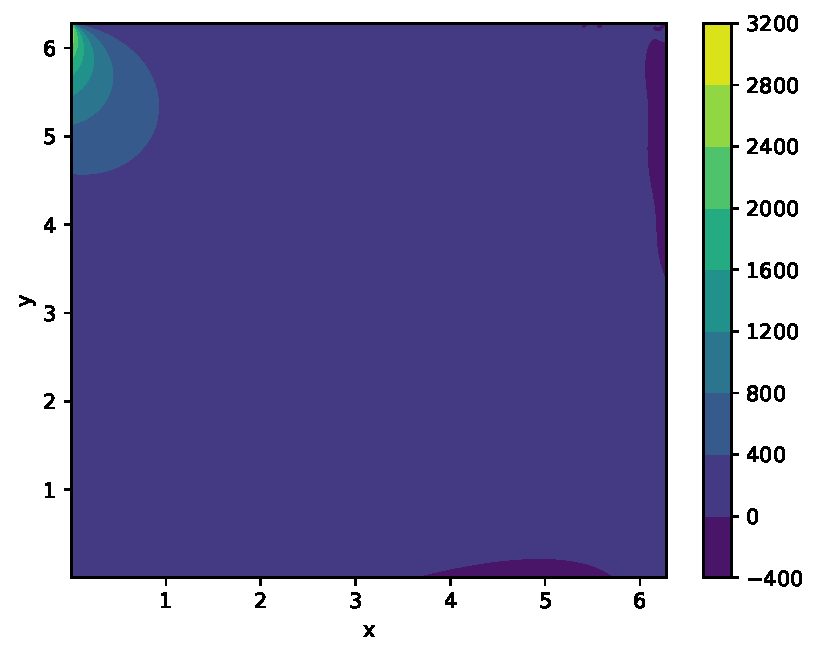
\includegraphics[width=\textwidth]{Figures/PINN-BO/heat_py_pde_1000_test_1.pdf}
%         \caption{Solution of Temperature Equation with boundary conditions 1}
%  \label{fig:heat_1_dist}
%     \end{subfigure}
%     \hfill
%     \begin{subfigure}[b]{0.3\textwidth}
%         \centering
%         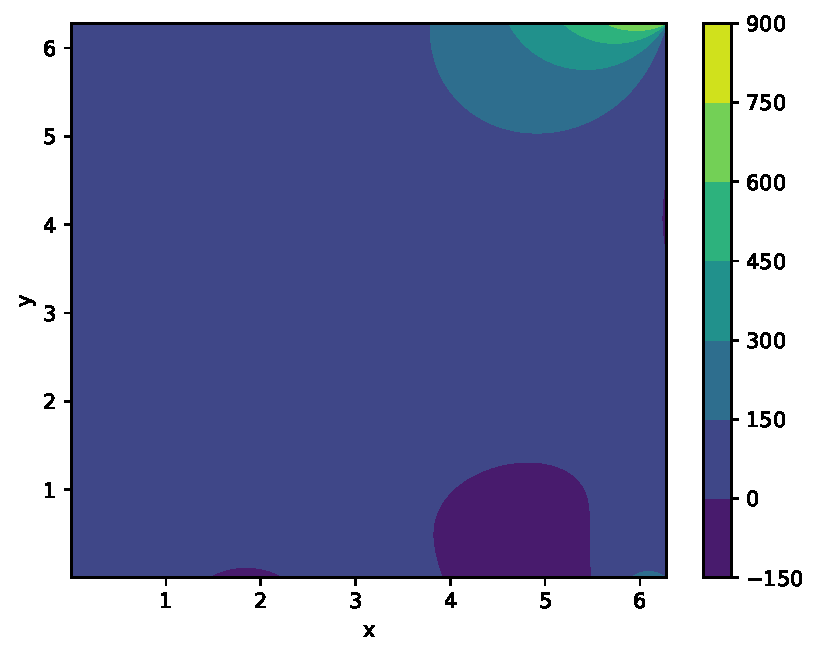
\includegraphics[width=1\textwidth]{Figures/PINN-BO/heat_py_pde_1000_test_2.pdf}
%         \caption{Solution of Temperature Equation with boundary conditions 2}
%         \label{fig:heat_2_dist}
%     \end{subfigure}
%     \hfill
%     \begin{subfigure}[b]{0.3\textwidth}
%         \centering
%         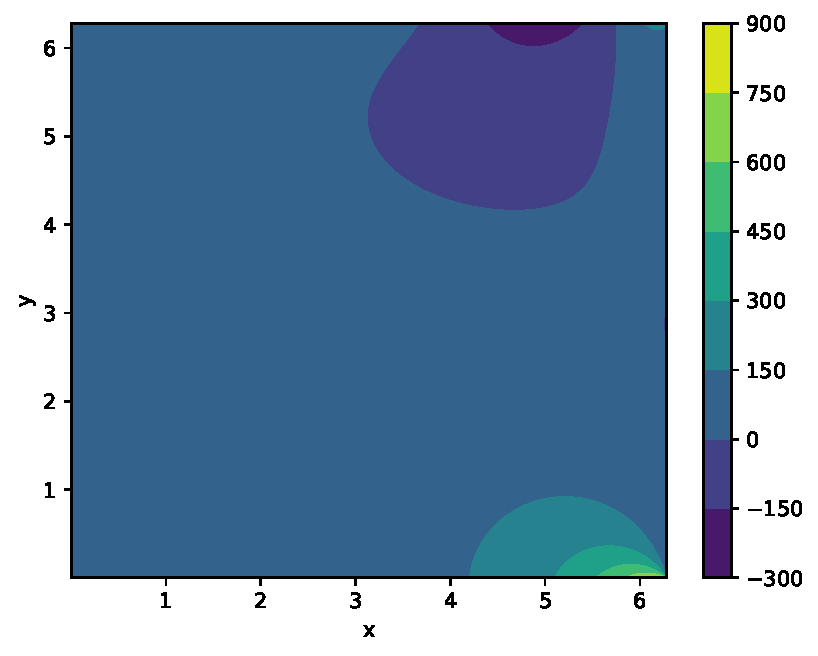
\includegraphics[width=\textwidth]{Figures/PINN-BO/heat_py_pde_1000_test_3.pdf}
%         \caption{Solution of Temperature Equation with boundary conditions 3}
%         \label{fig:heat_3_dist}
%     \end{subfigure}
%     \caption{The figures depict the solutions for temperature distributions governed by the heat equation, with each figure corresponding to a specific tuple of boundary conditions described in Section \ref{section:pinn-bo_experiments_2d_laplace}. It is evident that the region with the highest temperature is relatively small in comparison to the entire domain.}
%     \label{fig:heat_dist}
% \end{figure}

% We conducted temperature optimization by identifying the locations $(x,y)$ where the temperature reaches its maximum. As illustrated in Figure \ref{fig:heat_dist}, the area with high temperatures is relatively small in comparison to the regions with medium or low temperatures. For each baseline, we performed the optimization process 10 times, computing the average results. The comparative outcomes are presented in Figure \ref{fig:heat_opt}. 
% \begin{figure}[ht]
%     \centering
%     \begin{subfigure}[b]{0.3\textwidth}
%         \centering
%     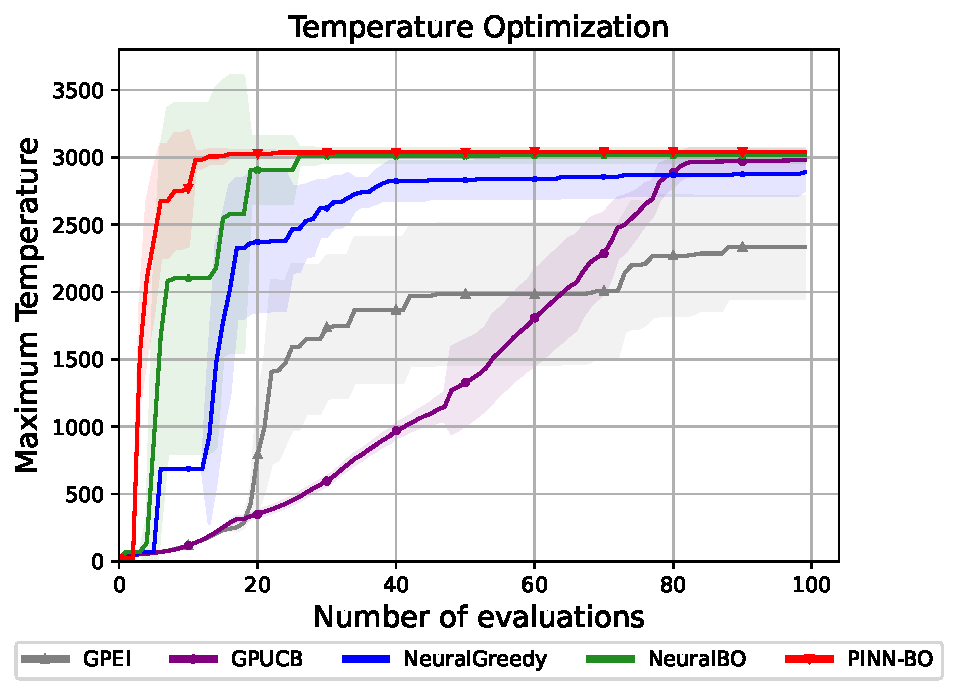
\includegraphics[width=\textwidth]{Figures/PINN-BO/Heat_dim_2_bc1.pdf}
%         \caption{Temperature Optimization in case of boundary conditions 1}
%  \label{fig:heat_1_opt}
%     \end{subfigure}
%     \hfill
%     \begin{subfigure}[b]{0.3\textwidth}
%         \centering
%         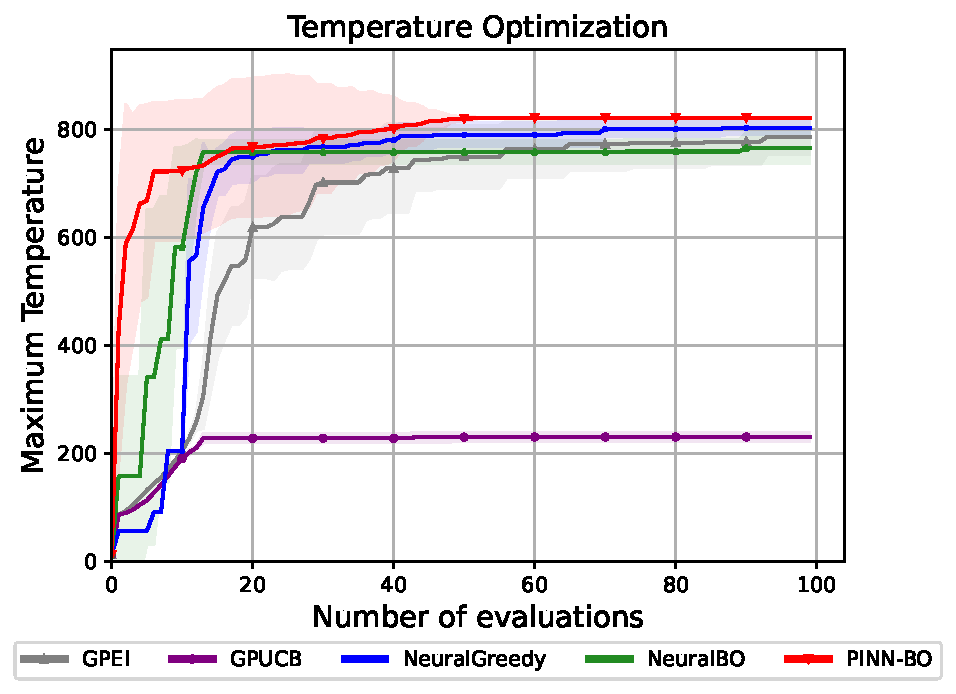
\includegraphics[width=1\textwidth]{Figures/PINN-BO/Heat_dim_2_bc2.pdf}
%         \caption{Temperature Optimization in case of boundary conditions 2}
%         \label{fig:heat_2_opt}
%     \end{subfigure}
%     \hfill
%     \begin{subfigure}[b]{0.3\textwidth}
%         \centering
%         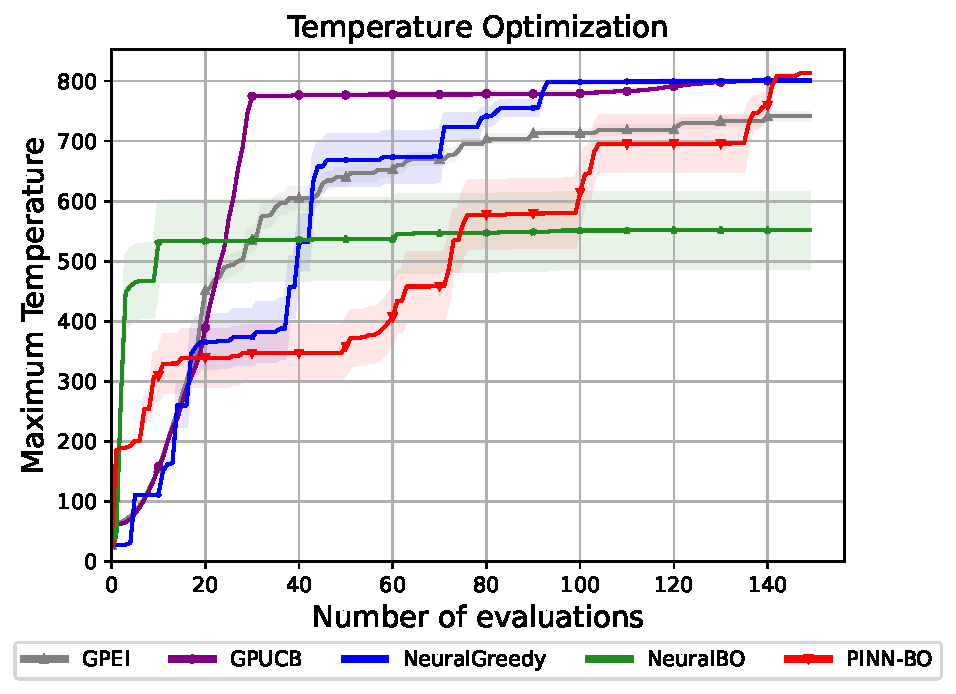
\includegraphics[width=\textwidth]{Figures/PINN-BO/Heat_dim_2_bc3.pdf}
%         \caption{Temperature Optimization in case of boundary conditions 3}
%         \label{fig:heat_3_opt}
%     \end{subfigure}
%     \caption{The figure shows the temperature optimization results of our PINN-BO and other baselines. For all three cases with different positions of maximum temperature, our PINN-BO performs better than all other baselines.}
%     \label{fig:heat_opt}
% \end{figure}


% \subsubsection{Optimizing Beam Displacement}
% We showcase the benchmark optimization outcomes obtained through our proposed method, PINN-BO, and the baseline approaches, addressing the task of minimizing the deflection of a non-uniform Euler-Bernoulli beam. The governing differential equation describing the behavior of a non-uniform Euler-Bernoulli beam is provided below: 
% \begin{equation*}
%     \frac{d^2}{dx^2} \left( EI(x) \frac{d^2 w(x)}{dx^2} \right) = q(x),
% \end{equation*}
% where
% $EI(x)$ represents the flexural rigidity of the beam, which can vary with position $x$, and $w(x)$ represents the vertical displacement of the beam at position $x$ and 
% $q(x)$ represents the distributed or concentrated load applied to the beam. 
% In our implementation, we consider the detailed expression of $EI(x)$ and $q(x)$ as follows:
% \begin{align*}
%     EI(x) &= \frac{e^x}{\rho(x)},\\
%     \rho(x) &= 2.4 x - 64 \pi^{2} e^{4 x} \sin{\left(4 \pi e^{2 x} \right)} - 396 e^{2 x} \sin{\left(20 x \right)} \\
%     &+ 80 e^{2 x} \cos{\left(20 x \right)} + 16 \pi e^{2 x} \cos{\left(4 \pi e^{2 x} \right)} + 0.4
% \end{align*}
% We employed the Finite Difference Method (FDM) to solve the non-uniform Euler-Bernoulli beam equation. It's crucial to note that this step is solely for generating observations at each input point. Despite obtaining this solution, our methods and all baseline techniques continue to treat this solution as a black-box function, accessing observations solely through querying. In Figure \ref{fig:beam_illustration}, the displacement values $w(x)$ for $x \in (0,1)$ are illustrated. The optimization results for both our PINN-BO and the other baseline methods are presented in Figure \ref{fig:beam_opt}.

% \begin{figure}[ht]
%     \centering
%     \begin{subfigure}[b]{0.44\textwidth}
%         \centering
%     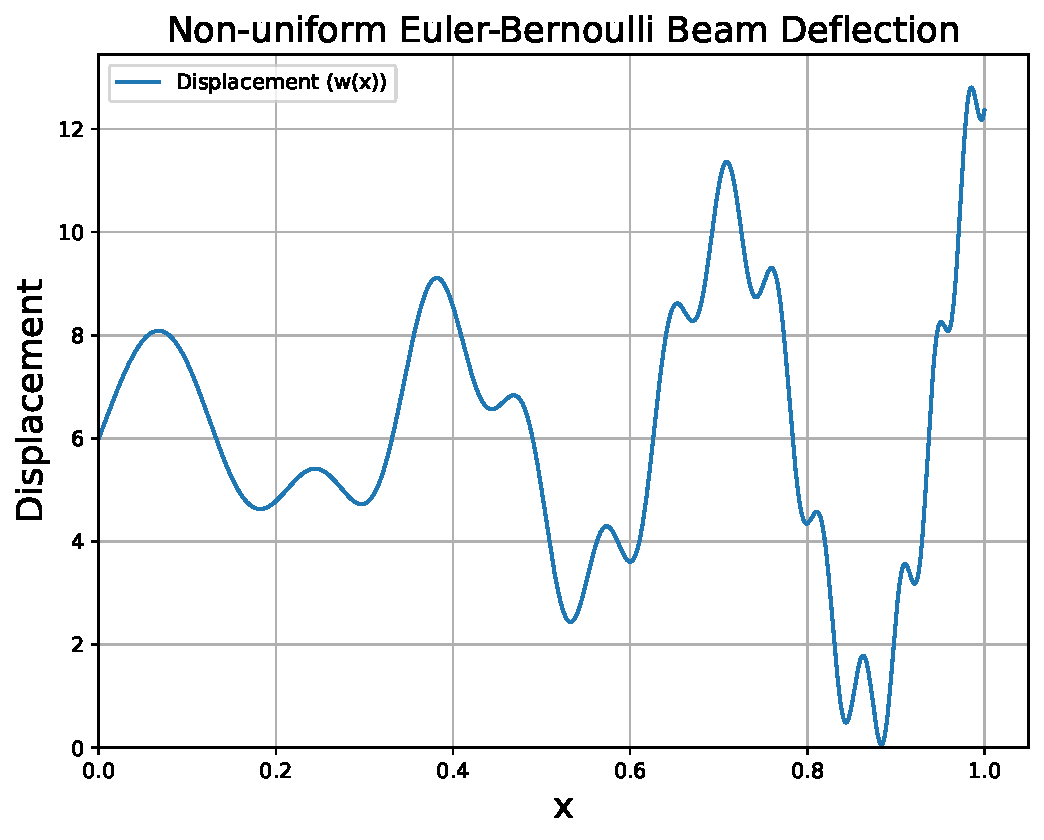
\includegraphics[width=\textwidth]{Figures/PINN-BO/beam.pdf}
%     \caption{Displacement of non-uniform Euler beam}
%      \label{fig:beam_illustration}
%     \end{subfigure}
%     \hfill
%     \begin{subfigure}[b]{0.49\textwidth}
%         \centering
%         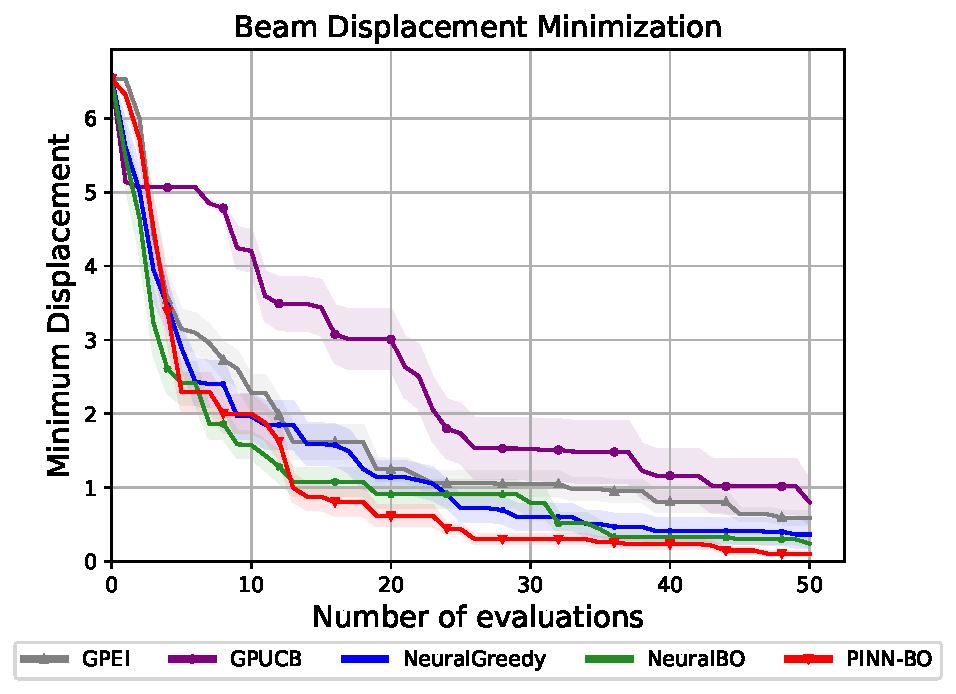
\includegraphics[width=1\textwidth]{Figures/PINN-BO/BeamDeflection_dim_1.pdf}
%         \caption{Displacement Optimization of non-uniform Euler beam}
%         \label{fig:beam_opt}
%     \end{subfigure}
%     \caption{Displacement of a Non-uniform Euler Beam and minimum displacement found by our PINN-BO and the other baselines. The left panel illustrates the natural displacement profile of the non-uniform Euler beam under given loads $q(x)$,  flexural rigidity $EI(x)$, and boundary conditions. The right panel depicts the optimized position on the beam where the displacement is minimized, highlighting the location where the structural response is at its lowest. }
%     \label{fig:beam}
% \end{figure}
\section{Proof of Theoretical Analysis in Chapter \ref{chap:pinn-bo}}
\label{section:pinn-bo_appendix}

\subsection{Proof of Lemma \ref{lemma:pinn-bo_PINN_mean_cov}}
In this section, we present the detailed proof of Lemma \ref{lemma:pinn-bo_PINN_mean_cov} in the main paper. Before going to the proof, we repeat Lemma \ref{lemma:pinn-bo_PINN_mean_cov} here:
\PinnMeanCov*

\textbf{To prove Lemma \ref{lemma:pinn-bo_PINN_mean_cov}, we need the following lemma:}

\begin{lemma}{(Theorem 4.1 \citet{wang2022and})}
\label{lemma:PINN_GP}
A sufficiently wide physics-informed neural network for modeling the problem defined in Section 4 induces a joint multivariate
Gaussian distribution between the network outputs and its ``derivatives'' after applying the differential operator to this network
\begin{align}
    \begin{bmatrix}
        \mathbf{h}_{\boldsymbol{\theta}} \\
        \mathbf{g}_{\boldsymbol{\theta}} 
\end{bmatrix} \sim N(\mathbf{0}, \mathbf{K}_\mathrm{NTK-PINN}),
\end{align} 
where $\mathbf{K}_\mathrm{NTK-PINN} = \begin{bmatrix}
    \mathbf{K}_{uu} & \mathbf{K}_{ur} \\
    \mathbf{K}_{ru} & \mathbf{K}_{rr}
\end{bmatrix}$ is the NTK matrix of PINN, with
\begin{align}
    (\mathbf{K}_{uu})_{ij} &= \langle \phi(\mathbf{x}_i), \phi(\mathbf{x}_j) \rangle \\ 
    (\mathbf{K}_{ur})_{ij} &= \langle \phi(\mathbf{x}_i), \omega(\mathbf{z}_j) \rangle
    \\
    (\mathbf{K}_{uu})_{ij} &= \langle \omega(\mathbf{z}_i), \omega(\mathbf{z}_j) \rangle
    \\
    \mathbf{K}_{ru} &= \mathbf{K}_{ur}^\top, \\ 
    \mathbf{h}_{\boldsymbol{\theta}} &= [h(\mathbf{x}_1, \boldsymbol{\theta}), \dots, h(\mathbf{x}_t, \boldsymbol{\theta})]^\top
    \\
    \mathbf{g}_{\boldsymbol{\theta}} &= \left[\mathcal{N}[h](\mathbf{z}_1, \boldsymbol{\theta}), \dots, \mathcal{N}[h](\mathbf{z}_{N_r}, \boldsymbol{\theta}) \right]^\top
\end{align}
where $\mathbf{x}_i, \mathbf{x}_j \in \mathcal{D}_t$ and $\mathbf{z}_i, \mathbf{z}_j \in \mathcal{R}$ are two arbitrary points belonging to the set $\mathcal{R}$ defined in Algorithm 1 and $\mathcal{N}[h]$ denotes a differential operator of the neural network $h(\cdot, \boldsymbol{\theta})$ with respect to the input $\mathbf{x}$. 
\end{lemma}
\begin{subcorollary}
\label{corollary:pinn-bo_PINN_GP_func}
    The unknown reward function values $f_{1:t}$ and the PDE observations $g_{1:N_r}$ are jointly Gaussian with an initial prior distribution with zero mean and the covariance $\nu_t^2 \mathbf{K}_\mathrm{NTK-PINN}$, where $\nu_t$ is the exploration coefficient introduced in Section 4. 
    \begin{align}
    \begin{bmatrix}
        f_{1:t} \\
        g_{1:N_r}
\end{bmatrix} \sim N(\mathbf{0}, \nu_t^2 \mathbf{K}_\mathrm{NTK-PINN}),
\end{align} 
\end{subcorollary}

\begin{proof}[Proof of Corollary  \ref{corollary:pinn-bo_PINN_GP_func}]
The algorithm updates the neural network by minimizing the loss function: \begin{equation}
    \mathcal{L}(t) = \sum^{t-1}_{i=1} [y_i - \nu_t h(\mathbf{x}_i; \boldsymbol{\theta}_{t-1})]^2 + \sum^{N_r}_{j=1}[u_j - \nu_t \mathcal{N}[h](\mathbf{z}_j; \boldsymbol{\theta}_{t-1})]^2
\end{equation} 
As the function prediction and its ``derivatives" prediction of each observation $\mathbf{x}_i$ and $\mathbf{z}_j$ at iteration $t$ is modeled by $\nu_t h(\mathbf{x}_i; \boldsymbol{\theta}_{t-1})$ and $\nu_t \mathcal{N}[h](\mathbf{z}_j; \boldsymbol{\theta}_{t-1})$, it is clear to see, from Lemma \ref{lemma:PINN_GP}, that the function values of the unknown function $f$ can be assumed to follow a joint Gaussian prior with zero means and covariance matrix $\nu_t^2 \mathbf{K}_\mathrm{NTK-PINN}$. A similar argument can be applied to the function $g$, where $g(\cdot) = \mathcal{N}[f] (\cdot)$ with $\mathcal{N}[f]$ is a differential operator. We are now ready to prove \ref{lemma:pinn-bo_PINN_mean_cov}.
\end{proof} 
\begin{proof} [Proof of Lemma \ref{lemma:pinn-bo_PINN_mean_cov}]
From Corollary \ref{corollary:pinn-bo_PINN_GP_func}, the priors for values of both $f$ and $g$ follow a joint Gaussian distribution with kernel $\mathbf{K}_\mathrm{NTK-PINN}$. Let $\mathbf{K_x}$ be the NTK matrix between point $\mathbf{x}$ and all training data: $\mathbf{K}_x = \begin{bmatrix}
        \Sigma_a & \Sigma_b \\
        \Sigma_c & \Sigma_d
    \end{bmatrix} =\begin{bmatrix}
         \boldsymbol{\Phi}_t \phi(\mathbf{x}) & 
         \boldsymbol{\Phi}_t \omega(\mathbf{x}) \\
         \boldsymbol{\Omega}_r\phi(\mathbf{x}) &
          \boldsymbol{\Omega}_r  \omega(\mathbf{x})  \end{bmatrix}$. 
Then the the posterior of $f$ and $g$ evaluated at an input $\mathbf{x}$ will be a Gaussian distribution with mean and variance functions:
\paragraph{Mean function:}
\begin{align*}
    &\;\;\;\; \begin{bmatrix}
        \mu_t^f(\mathbf{x})\\
        \mu_t^g(\mathbf{x}) 
    \end{bmatrix} = \mathbf{K}_\mathbf{x} ^\top \mathbf{\widehat{K}}_\mathrm{PINN}^{-1} \begin{bmatrix}
        \mathbf{Y}_t \\
        \mathbf{U}_r
    \end{bmatrix}
    \\
    &= \begin{bmatrix}
        \Sigma_a^\top & \Sigma_c^\top \\
        \Sigma_b^\top & \Sigma_d^\top
    \end{bmatrix} \begin{bmatrix}
        \widetilde{\mathbf{A}} & \widetilde{\mathbf{B}} \\
    \widetilde{\mathbf{C}} & \widetilde{\mathbf{D}}
    \end{bmatrix} \begin{bmatrix}
        \mathbf{Y}_t \\
        \mathbf{U}_r
    \end{bmatrix}\\
    &= \begin{bmatrix}
        \phi(\mathbf{x})^\top \boldsymbol{\Phi}_t^\top &  \phi(\mathbf{x})^\top \boldsymbol{\Omega}_r ^\top \\
        \omega(\mathbf{x})^\top \boldsymbol{\Phi}_t^\top  & \omega(\mathbf{x})^\top \boldsymbol{\Omega}_r ^\top
    \end{bmatrix} \begin{bmatrix}
        \widetilde{\mathbf{A}} & \widetilde{\mathbf{B}} \\
    \widetilde{\mathbf{C}} & \widetilde{\mathbf{D}}
    \end{bmatrix} \begin{bmatrix}
        \mathbf{Y}_t \\
        \mathbf{U}_r
    \end{bmatrix} \\
    & = \begin{bmatrix}
         \phi(\mathbf{x})^\top \boldsymbol{\Phi}_t^\top \widetilde{\mathbf{A}}\mathbf{Y}_t +  \phi(\mathbf{x})^\top \boldsymbol{\Omega}_r ^\top  \widetilde{\mathbf{C}}\mathbf{Y}_t  + \phi(\mathbf{x})^\top \boldsymbol{\Phi}_t^\top \widetilde{\mathbf{B}} \mathbf{U}_r   +  \phi(\mathbf{x})^\top \boldsymbol{\Omega}_r ^\top  \widetilde{\mathbf{D}} \mathbf{U}_r \\
         \omega(\mathbf{x})^\top \boldsymbol{\Phi}_t^\top \widetilde{\mathbf{A}} \mathbf{Y}_t +  \omega(\mathbf{x})^\top \boldsymbol{\Omega}_r ^\top  \widetilde{\mathbf{C}} \mathbf{Y}_t  +\omega(\mathbf{x})^\top \boldsymbol{\Phi}_t^\top \widetilde{\mathbf{B}} \mathbf{U}_r  +  \omega(\mathbf{x})^\top \boldsymbol{\Omega}_r ^\top  \widetilde{\mathbf{D}} \mathbf{U}_r
    \end{bmatrix}
        \\
         &=\phi(\mathbf{x})^\top \boldsymbol{\xi}_t^\top \mathbf{\widehat{K}}_\mathrm{PINN}^{-1} \begin{bmatrix}
         \mathbf{Y}_t \\
         \mathbf{U}_r\end{bmatrix}
\end{align*}

\paragraph{Variance function:}
Let $\mathbf{K}_{\mathbf{xx}} = \begin{bmatrix}
\langle \phi(\mathbf{x}), \phi(\mathbf{x}) \rangle & \langle \phi(\mathbf{x}), \omega(\mathbf{x}) \rangle \\
\langle \omega(\mathbf{x}), \phi(\mathbf{x}) \rangle & \langle \omega(\mathbf{x}), \omega(\mathbf{x}) \rangle
\end{bmatrix}$, then we have the posterior covariance matrix of $f$ and $g$ at input $\mathbf{x}$ is:
\begin{align}
    &\begin{bmatrix}
    \mathrm{Cov}_f(\mathbf{x}) & \mathrm{Cov}_{fg}(\mathbf{x}) \\
    \mathrm{Cov}_{gf}(\mathbf{x}) & \mathrm{Cov}_g(\mathbf{x})
\end{bmatrix}  \\
&= \nu_t^2 \left(\mathbf{K}_{\mathbf{xx}} - \mathbf{K_x}^\top \mathbf{\widehat{K}}_\mathrm{PINN}^{-1} \mathbf{K_x} \right) \\
&= \nu_t^2   \begin{bmatrix}
\langle \phi(\mathbf{x}), \phi(\mathbf{x}) \rangle & \langle \phi(\mathbf{x}), \omega(\mathbf{x}) \rangle \notag \\
\langle \omega(\mathbf{x}), \phi(\mathbf{x}) \rangle & \langle \omega(\mathbf{x}), \omega(\mathbf{x}) \rangle
\end{bmatrix} - \nu_t^2
\begin{bmatrix}
        \Sigma_a^\top& \Sigma_c^\top \\
        \Sigma_b^\top & \Sigma_d^\top
\end{bmatrix} \begin{bmatrix}
    \widetilde{\mathbf{A}} & \widetilde{\mathbf{B}} \\
    \widetilde{\mathbf{C}} & \widetilde{\mathbf{D}}
        \end{bmatrix}  \begin{bmatrix}
                            \Sigma_a & \Sigma_b \\
                            \Sigma_c & \Sigma_d
                        \end{bmatrix}  \\
\end{align}
Therefore, 
\begin{align}
\mathrm{Cov}_f(\mathbf{x}) & = \nu_t^2 \langle \phi(\mathbf{x}),  \phi(\mathbf{x}) \rangle - \nu_t^2(\Sigma_a^\top \widetilde{\mathbf{A}}\Sigma_a + \Sigma_c^\top \widetilde{\mathbf{C}}\Sigma_c + \Sigma_a^\top \widetilde{\mathbf{B}}\Sigma_a + \Sigma_c^\top \widetilde{\mathbf{D}}\Sigma_c) \\
        & = \nu_t^2 \langle \phi(\mathbf{x}),  \phi(\mathbf{x}) \rangle - \nu_t^2 \begin{bmatrix}
            \Sigma_a^\top  & \Sigma_c^\top
        \end{bmatrix}
        \begin{bmatrix}
    \widetilde{\mathbf{A}} & \widetilde{\mathbf{B}} \\
    \widetilde{\mathbf{C}} & \widetilde{\mathbf{D}}
        \end{bmatrix} \begin{bmatrix}
            \Sigma_a \\ \Sigma_c
        \end{bmatrix}  \\
        &= \nu_t^2 \langle \phi(\mathbf{x}),  \phi(\mathbf{x}) \rangle - \nu_t^2\begin{bmatrix}
            \phi(\mathbf{x})^\top \boldsymbol{\Phi}_t^\top & \phi(\mathbf{x})^\top \boldsymbol{\Omega}_r^\top
        \end{bmatrix}  \begin{bmatrix}
    \widetilde{\mathbf{A}} & \widetilde{\mathbf{B}} \\
    \widetilde{\mathbf{C}} & \widetilde{\mathbf{D}}
        \end{bmatrix} \begin{bmatrix} \boldsymbol{\Phi}_t \phi(\mathbf{x}) \\ \boldsymbol{\Omega}_r \phi(\mathbf{x})  \end{bmatrix}  \\
        &= \nu_t^2 \langle \phi(\mathbf{x}),  \phi(\mathbf{x}) \rangle - \nu_t^2\phi(\mathbf{x})^\top \boldsymbol{\xi}_t^\top \mathbf{\widehat{K}}_\mathrm{PINN}^{-1} \boldsymbol{\xi}_t \phi(\mathbf{x})\\
        &= \nu_t^2 (\sigma_t^f)^2(\mathbf{x})
\end{align}
\end{proof}
\subsection{Proof of Lemma \ref{lemma:interaction_information_formula}}
\begin{lemma}
    \label{lemma:interaction_information_formula}
    The interaction information between $f$ and observation $\mathbf{Y}_t$ and PDE data $\mathbf{U}_r$, for the points chosen from Algorithm 1 can be calculated as:
    \begin{equation*}
        I (f; \mathbf{Y}_t; \mathbf{U}_r) = \frac{1}{2}  \log (\frac{\det(\frac{\boldsymbol{\Phi}_t^\top \boldsymbol{\Phi}_t}{\lambda_1} + \mathbf{I})\det(\frac{\boldsymbol{\Omega}_r^\top \boldsymbol{\Omega}_r}{\lambda_2} + \mathbf{I})}{\det(\frac{\boldsymbol{\Phi}_t^\top \boldsymbol{\Phi}_t}{\lambda_1} + \frac{\boldsymbol{\Omega}_r^\top \boldsymbol{\Omega}_r}{\lambda_2} + \mathbf{I})})
    \end{equation*}
\end{lemma}
\textbf{To prove Lemma \ref{lemma:interaction_information_formula}, we need to prove the following technical lemma:}
\begin{sublemma}    \label{lemma:det_division}
    Let $\mathbf{u} \in \mathrm{R}^{n \times p}$ and $\mathbf{K} \in \mathrm{R}^{p \times p}$ is a positive semi-definite matrix and $p \ge n$. Then 
    \begin{align}
    \frac{\det [\mathbf{u}\left(\mathbf{K}(\mathbf{u}^\top\mathbf{u}+\mathbf{I})^{-1} + \mathbf{I}\right)^{-1}\mathbf{u}^\top]}{[\mathbf{u}\left(\mathbf{K} + \mathbf{I}\right)^{-1}\mathbf{u}^\top]} =  \frac{\det \left(\mathbf{K}(\mathbf{u}^\top\mathbf{u}+\mathbf{I})^{-1} + \mathbf{I}\right)^{-1}}{\det \left(\mathbf{K} + \mathbf{I}\right)^{-1}}   
    \end{align}
\end{sublemma}
\begin{proof}[Proof of Lemma \ref{lemma:det_division}]
We start the proof by gradually calculating the denominator and numerator.
\paragraph{Denominator}

\begin{align*}
&\det[\mathbf{u} (\mathbf{I} + \mathbf{K})^{-1} \mathbf{u}^\top] \\ &= \det [\mathbf{u} \left[ (\mathbf{I} - \mathbf{K}(\mathbf{I}+\mathbf{K})^{-1}\right]\mathbf{u}^\top]\\
&=\det [\mathbf{u} \mathbf{u}^\top - \mathbf{u} \mathbf{K}(\mathbf{I}+\mathbf{K})^{-1} \mathbf{u}^\top]  \\
&= \det \left[  (\mathbf{u} \mathbf{u}^\top) \left(\mathbf{K}(\mathbf{I}+\mathbf{K})^{-1}\right) \left( (\mathbf{I} + \mathbf{K}) \mathbf{K}^{-1} - \mathbf{u}^\top (\mathbf{u} \mathbf{u}^\top)^{-1} \mathbf{u}\right) \right] \\
&= \det (\mathbf{u} \mathbf{u}^\top) \det \left(\mathbf{K}(\mathbf{I}+\mathbf{K})^{-1}\right) \det \left( (\mathbf{I} + \mathbf{K}) \mathbf{K}^{-1} - \mathbf{u}^\top (\mathbf{u} \mathbf{u}^\top)^{-1} \mathbf{u}\right) \\
&= \det (\mathbf{u} \mathbf{u}^\top) \det \left((\mathbf{I}+\mathbf{K})^{-1}\right) \det \mathbf{K} \det \left( (\mathbf{I} + \mathbf{K}) \mathbf{K}^{-1} - \mathbf{u}^\top (\mathbf{u} \mathbf{u}^\top)^{-1} \mathbf{u}\right) \\
& = \det (\mathbf{u} \mathbf{u}^\top) \det \left((\mathbf{I}+\mathbf{K})^{-1}\right) \det \left( \mathbf{K}(\mathbf{I} + \mathbf{K}) \mathbf{K}^{-1} - \mathbf{K}\mathbf{u}^\top (\mathbf{u} \mathbf{u}^\top)^{-1} \mathbf{u}\right) \\
\label{Eqn:u_K_inv_uT}
& = \det (\mathbf{u} \mathbf{u}^\top) \det \left((\mathbf{I}+\mathbf{K})^{-1}\right) \det \left(\mathbf{I} + \mathbf{K} - \mathbf{K}\mathbf{u}^\top (\mathbf{u} \mathbf{u}^\top)^{-1} \mathbf{u}\right)
\end{align*}
The first equation utilizes the Woodbury matrix inversion formula while the third equation uses generalized matrix determinant lemma \footnote{Suppose $\mathbf{A}$ is an invertible $n$-by-$n$ matrix and $\mathbf{U}, \mathbf{V}$ are $n$-by-$m$ matrices, $m \le n$. Then $\det(\mathbf{A} + \mathbf{U}\mathbf{W}\mathbf{V}^\top) = \det(\mathbf{A}) \det(\mathbf{W})\det(\mathbf{W}^{-1} + \mathbf{V}^\top \mathbf{A}^{-1} \mathbf{U})$.}.
\paragraph{Numerator}
Let $\widetilde{\mathbf{K}} = \mathbf{K} (\mathbf{u}^\top \mathbf{u} + \mathbf{I})^{-1}$, then we have
\begin{align}
    &\det [\mathbf{u}\left(\mathbf{K}(\mathbf{u}^\top\mathbf{u}+\mathbf{I})^{-1} + \mathbf{I}\right)^{-1}\mathbf{u}^\top] 
    \\
    &= \det [\mathbf{u}\left( \mathbf{I}+\widetilde{\mathbf{K}} \right)^{-1}\mathbf{u}^\top] \\
    & = \det (\mathbf{u} \mathbf{u}^\top) \det \left((\mathbf{I}+\widetilde{\mathbf{K}})^{-1}\right) \det \left( \mathbf{I} + \widetilde{\mathbf{K}} - \widetilde{\mathbf{K}}\mathbf{u}^\top (\mathbf{u} \mathbf{u}^\top)^{-1} \mathbf{u}\right),
\end{align}
where we use the result at line  (\ref{Eqn:u_K_inv_uT}) and replace $\mathbf{K}$ by $\widetilde{\mathbf{K}}$. We also have: 
\begin{align}
    &\det \left( (\mathbf{I} + \widetilde{\mathbf{K}}) - \widetilde{\mathbf{K}}\mathbf{u}^\top (\mathbf{u} \mathbf{u}^\top)^{-1} \mathbf{u}\right) \\
    = &\det \left( \mathbf{I} + \mathbf{K} (\mathbf{u}^\top \mathbf{u} + \mathbf{I})^{-1} - \mathbf{K} (\mathbf{u}^\top \mathbf{u} + \mathbf{I})^{-1}\mathbf{u}^\top (\mathbf{u} \mathbf{u}^\top)^{-1} \mathbf{u}\right) \\
    = &  \det \left[ \mathbf{I} + \mathbf{K} \left( \mathbf{I} - \mathbf{u}^\top \mathbf{u} (\mathbf{u}^\top \mathbf{u} + \mathbf{I})^{-1} \right) - \mathbf{K} (\mathbf{u}^\top \mathbf{u} + \mathbf{I})^{-1}\mathbf{u}^\top (\mathbf{u} \mathbf{u}^\top)^{-1} \mathbf{u}\right] \\
    = &  \det \left[ \mathbf{I} + \mathbf{K} - \mathbf{K} \mathbf{u}^\top \mathbf{u} (\mathbf{u}^\top \mathbf{u} + \mathbf{I})^{-1}  - \mathbf{K} (\mathbf{u}^\top \mathbf{u} + \mathbf{I})^{-1}\mathbf{u}^\top (\mathbf{u} \mathbf{u}^\top)^{-1} \mathbf{u}\right] \\
    = &  \det \left[ \mathbf{I} + \mathbf{K} - \mathbf{K} \mathbf{u}^\top (\mathbf{u} \mathbf{u}^\top + \mathbf{I})^{-1}\mathbf{u}  - \mathbf{K} \mathbf{u}^\top ( \mathbf{u}\mathbf{u}^\top + \mathbf{I})^{-1} (\mathbf{u} \mathbf{u}^\top)^{-1} \mathbf{u}\right] \\ 
    = &  \det \left[ \mathbf{I} + \mathbf{K} - \mathbf{K} \mathbf{u}^\top (\mathbf{u} \mathbf{u}^\top + \mathbf{I})^{-1} \left( \mathbf{I} + (\mathbf{u} \mathbf{u}^\top)^{-1} \right)  \mathbf{u} \right] \\ 
    = &  \det \left( \mathbf{I} + \mathbf{K} - \mathbf{K} \mathbf{u}^\top (\mathbf{u} \mathbf{u}^\top)^{-1}  \mathbf{u} \right)
\end{align}
Therefore, we have the final expression of the numerator  
\begin{align}
    &\det \left( (\mathbf{I} + \widetilde{\mathbf{K}}) - \widetilde{\mathbf{K}}\mathbf{u}^\top (\mathbf{u} \mathbf{u}^\top)^{-1} \mathbf{u}\right) 
    \\
    &= \det (\mathbf{u} \mathbf{u}^\top) \det \left((\mathbf{I}+\widetilde{\mathbf{K}})^{-1}\right) \det \left( \mathbf{I} + \mathbf{K} - \mathbf{K} \mathbf{u}^\top (\mathbf{u} \mathbf{u}^\top)^{-1}  \mathbf{u} \right)
\end{align}
Using the derived numerator and denominator, we have 
\begin{align}
    & \frac{\det [\mathbf{u}\left(\mathbf{K}(\mathbf{u}^\top\mathbf{u}+\mathbf{I})^{-1} + \mathbf{I}\right)^{-1}\mathbf{u}^\top]}{[\mathbf{u}\left(\mathbf{K} + \mathbf{I}\right)^{-1}\mathbf{u}^\top]} 
    \\
    &= \frac{\det (\mathbf{u} \mathbf{u}^\top) \det \left((\mathbf{I}+\widetilde{\mathbf{K}})^{-1}\right) \det \left( \mathbf{I} + \mathbf{K} - \mathbf{K} \mathbf{u}^\top (\mathbf{u} \mathbf{u}^\top)^{-1}  \mathbf{u} \right)}{\det (\mathbf{u} \mathbf{u}^\top) \det \left((\mathbf{I}+\mathbf{K})^{-1}\right) \det \left(\mathbf{I} + \mathbf{K} - \mathbf{K}\mathbf{u}^\top (\mathbf{u} \mathbf{u}^\top)^{-1} \mathbf{u}\right)}\\
    &=\frac{\det (\mathbf{I}+\widetilde{\mathbf{K}})^{-1}}{\det (\mathbf{I}+\mathbf{K})^{-1}} \\
    &=\frac{\det \left(\mathbf{K}(\mathbf{u}^\top\mathbf{u}+\mathbf{I})^{-1} + \mathbf{I}\right)^{-1}}{\det \left(\mathbf{K} + \mathbf{I}\right)^{-1}}   
    \end{align} 
\end{proof}
\begin{subcorollary}
\label{corollary:det_divison_corollary}
Let $\mathbf{u} \in \mathrm{R}^{n \times p}$ and $\mathbf{K} \in \mathrm{R}^{p \times p}$ is a positive semi-definite matrix and $p \ge n$. Then 
\begin{align}
    \frac{\det[\mathbf{u}(\mathbf{K}+\mathbf{I})^{-1} \mathbf{u}^\top]}{\det [\mathbf{u}(\mathbf{K}+ \mathbf{u}^\top \mathbf{u} + \mathbf{I})^{-1} \mathbf{u}^\top]} = \frac{\det (\mathbf{K}+\mathbf{I})^{-1}}{\det(\mathbf{K}+\mathbf{u}^\top \mathbf{u}+\mathbf{I})^{-1}}
\end{align}
\end{subcorollary}
\begin{proof} [Proof of Corollary \ref{corollary:det_divison_corollary}]
    \begin{align}
        & \frac{\det[\mathbf{u}(\mathbf{K}+\mathbf{I})^{-1} \mathbf{u}^\top]}{\det [\mathbf{u}(\mathbf{K}+ \mathbf{u}^\top \mathbf{u} + \mathbf{I})^{-1} \mathbf{u}^\top]} \notag
        \\
        &= \frac{\det[\mathbf{u}(\mathbf{K}+\mathbf{I})^{-1} \mathbf{u}^\top]}{\det [\mathbf{u} (\mathbf{u}^\top \mathbf{u}+\mathbf{I})^{-1}(\mathbf{K} (\mathbf{u}^\top \mathbf{u} + \mathbf{I})^{-1} + \mathbf{I})^{-1} \mathbf{u}^\top]}
        \\
        &=\frac{\det[\mathbf{u}(\mathbf{K}+\mathbf{I})^{-1} \mathbf{u}^\top]}{\det [ (\mathbf{u} \mathbf{u}^\top+\mathbf{I})^{-1}\mathbf{u} (\mathbf{K} (\mathbf{u}^\top \mathbf{u} + \mathbf{I})^{-1} + \mathbf{I})^{-1} \mathbf{u}^\top]}
        \\
        &= \frac{1}{\det (\mathbf{u} \mathbf{u}^\top+\mathbf{I})^{-1}} \frac{\det[\mathbf{u}(\mathbf{K}+\mathbf{I})^{-1} \mathbf{u}^\top]}{\det [\mathbf{u} (\mathbf{K} (\mathbf{u}^\top \mathbf{u} + \mathbf{I})^{-1} + \mathbf{I})^{-1} \mathbf{u}^\top]}
        \\
        &=\frac{1}{\det (\mathbf{u} ^\top \mathbf{u}+\mathbf{I})^{-1}} \frac{\det[(\mathbf{K}+\mathbf{I})^{-1}]}{\det [ (\mathbf{K} (\mathbf{u}^\top \mathbf{u} + \mathbf{I})^{-1} + \mathbf{I})^{-1}]}
        \\
        &= \frac{\det (\mathbf{K}+\mathbf{I})^{-1}}{\det(\mathbf{K}+\mathbf{u}^\top \mathbf{u}+\mathbf{I})^{-1}},
    \end{align}
The second equation uses the matrix inversion identity of two non-singular matrices $\mathbf{A}$ and $\mathbf{B}$, i.e., $(\mathbf{A}\mathbf{B})^{-1} = \mathbf{B}^{-1} \mathbf{A}^{-1}$ while the fourth equation directly utilizes Lemma \ref{lemma:det_division}.
\end{proof}
\begin{proof}[Proof of Lemma \ref{lemma:interaction_information_formula}]
By definition, we have $I (f; \mathbf{Y}_t; \mathbf{U}_r) = I(f; \mathbf{Y}_t) - I (f; \mathbf{Y}_t \rvert \mathbf{U}_r)$. We start by proof by calculating $I (f; \mathbf{Y}_t \rvert \mathbf{U}_r)$.

By the properties of GPs, given a set of sampling points $\mathcal{D}_t\subset \mathcal{D}$, we have that $f, \mathbf{Y}_t, \mathbf{U}_r$ are jointly Gaussian:
\begin{align}
\label{Eqn:joint_gauss_3_variables}
\left(
\begin{aligned}
    f\\
    \mathbf{Y}_t\\
    \mathbf{U}_r
\end{aligned}
\right) \sim \mathcal{N} \left(\mathbf{0}, \nu_t^2 \begin{bmatrix}
    \mathbf{K}_{uu} & \mathbf{K}_{uu} & \mathbf{K}_{ur} \\
    \mathbf{K}_{uu} & \mathbf{K}_{uu} + \lambda_1 \mathbf{I} & \mathbf{K}_{ur} \\
    \mathbf{K}_{ru} & \mathbf{K}_{uu} & \mathbf{K}_{rr} + \lambda_2 \mathbf{I}
\end{bmatrix} \right)    
\end{align} 


Then, we have
\begin{align}
    \textup{Cov}(f \rvert \mathbf{U}_r) &=  \nu_t^2 \left[ \mathbf{K}_{uu} - \mathbf{K}_{ur}(\mathbf{K}_{rr}+ \lambda_2\mathbf{I})^{-1} \mathbf{K}_{ru} \right]
        \\
        &= \nu_t^2 \left[\boldsymbol{\Phi}_t \boldsymbol{\Phi}_t^\top - \boldsymbol{\Phi}_t\boldsymbol{\Omega}_r^\top (\boldsymbol{\Omega}_r\boldsymbol{\Omega}_r^\top + \lambda_2\mathbf{I})^{-1} \boldsymbol{\Omega}_r\boldsymbol{\Phi}_t^\top \right]
        \\
        &= \nu_t^2 \left[\boldsymbol{\Phi}_t\boldsymbol{\Phi}_t^\top - \boldsymbol{\Phi}_t\left[\mathbf{I} - \lambda_2(\boldsymbol{\Omega}_r\boldsymbol{\Omega}_r^\top + \lambda_2\mathbf{I})^{-1}\right] \boldsymbol{\Phi}_t^\top \right] 
        \\
        &= \nu_t^2 \lambda_2 \boldsymbol{\Phi}_t (\boldsymbol{\Omega}_r^\top \boldsymbol{\Omega}_r + \lambda_2\mathbf{I})^{-1} \boldsymbol{\Phi}_t^\top
        \\ \label{Eqn:covar_f_condition_on_u}
        &= \nu_t^2 \boldsymbol{\Phi}_t \left(\frac{\boldsymbol{\Omega}_r^\top \boldsymbol{\Omega}_r}{\lambda_2} + \mathbf{I}\right)^{-1} \boldsymbol{\Phi}_t^\top,
\end{align}
and 
\begin{align}
\label{Eqn:covar_f_condition_on_y_and_u}
        \textup{Cov}(f \rvert \mathbf{Y}_t; \mathbf{U}_r) &= \nu_t^2 \left(\mathbf{K}_{uu} - \begin{bmatrix}
            \mathbf{K}_{uu} & \mathbf{K}_{ur}
        \end{bmatrix} \begin{bmatrix}
            \mathbf{K}_{uu} + \lambda_1\mathbf{I} & \mathbf{K}_{ur} \\
            \mathbf{K}_{ru} & \mathbf{K}_{rr} + \lambda_2 \mathbf{I}
        \end{bmatrix}^{-1} \begin{bmatrix}
            \mathbf{K}_{uu} \\
            \mathbf{K}_{ru}
        \end{bmatrix} \right) \\
        & = \nu_t^2 (\boldsymbol{\Phi}_t \boldsymbol{\Phi}_t^\top - \boldsymbol{\Phi}_t \boldsymbol{\xi}_t^\top \mathbf{\widehat{K}}_\mathrm{PINN}^{-1} \boldsymbol{\xi}_t \boldsymbol{\Phi}_t^\top) 
\end{align}
Let $\mathbf{V} = \boldsymbol{\xi}_t^\top \mathbf{\widehat{K}}_\mathrm{PINN}^{-1} \boldsymbol{\xi}_t$, now we need to calculate $\mathbf{V}$. We have
    \begin{align}
            \mathbf{V} &= \boldsymbol{\boldsymbol{\xi}_t}^\top \mathbf{\widehat{K}}_\mathrm{PINN}^{-1} \boldsymbol{\boldsymbol{\xi}_t} \\
            &=\boldsymbol{\Phi}_t^\top \widetilde{\mathbf{A}}\boldsymbol{\Phi}_t + \boldsymbol{\Omega}_r^\top \widetilde{\mathbf{C}}\boldsymbol{\Phi}_t + \boldsymbol{\Phi}_t^\top \widetilde{\mathbf{B}}\boldsymbol{\Omega}_r + \boldsymbol{\Omega}_r^\top \widetilde{\mathbf{D}}\boldsymbol{\Omega}_r \\
            & = \boldsymbol{\Phi}_t^\top (\mathbf{P}^{-1} - \mathbf{P}^{-1}\mathbf{Q}\widetilde{\mathbf{C}})\boldsymbol{\Phi}_t + \boldsymbol{\Omega}_r^\top \widetilde{\mathbf{C}}\boldsymbol{\Phi}_t - \boldsymbol{\Phi}_t^\top \mathbf{P}^{-1}\mathbf{Q}\boldsymbol{\Omega}_r + \boldsymbol{\Omega}_r^\top \widetilde{\mathbf{D}}\boldsymbol{\Omega}_r \\
            & = \boldsymbol{\Phi}_t^\top \mathbf{P}^{-1}\boldsymbol{\Phi}_t - \boldsymbol{\Phi}_t^\top\mathbf{P}^{-1}\mathbf{Q}\widetilde{\mathbf{C}}\boldsymbol{\Phi}_t + \boldsymbol{\Omega}_r^\top \widetilde{\mathbf{C}}\boldsymbol{\Phi}_t - \boldsymbol{\Phi}_t^\top \mathbf{P}^{-1}\mathbf{Q}\boldsymbol{\Omega}_r + \boldsymbol{\Omega}_r^\top \widetilde{\mathbf{D}}\boldsymbol{\Omega}_r \\
            & = \boldsymbol{\Phi}_t^\top \mathbf{P}^{-1}\boldsymbol{\Phi}_t + (\underbrace{\boldsymbol{\Omega}_r - \boldsymbol{\Phi}_t^\top\mathbf{P}^{-1}\mathbf{Q}}_{U_1})(\widetilde{\mathbf{C}}\boldsymbol{\Phi}_t + \widetilde{\mathbf{D}}\boldsymbol{\Omega}_r) \\
            & = \boldsymbol{\Phi}_t^\top \mathbf{P}^{-1}\boldsymbol{\Phi}_t + (\underbrace{\boldsymbol{\Omega}_r - \boldsymbol{\Phi}_t^\top\mathbf{P}^{-1}\mathbf{Q}}_{V_1})(\underbrace{\widetilde{\mathbf{C}}\boldsymbol{\Phi}_t + \widetilde{\mathbf{D}}\boldsymbol{\Omega}_r)}_{V_2} \\
            & = \boldsymbol{\Phi}_t^\top (\boldsymbol{\Phi}_t\boldsymbol{\Phi}_t^\top+\lambda_1 \mathbf{I})^{-1} \boldsymbol{\Phi}_t + V_1V_2\\
            & = (\boldsymbol{\Phi}_t^\top\boldsymbol{\Phi}_t+\lambda_1 \mathbf{I})^{-1} \boldsymbol{\Phi}_t^\top\boldsymbol{\Phi}_t + V_1V_2
    \end{align}
    where 
    \begin{align}
            \label{terms:pqrs}
            \begin{bmatrix}
            \mathbf{P} & \mathbf{Q} \\
            \mathbf{R} & \mathbf{S}
            \end{bmatrix} & = \begin{bmatrix}
            \mathbf{K}_{uu} + \lambda_1\mathbf{I} & \mathbf{K}_{ur}  \\
            \mathbf{K}_{ru}  & \mathbf{K}_{rr} + \lambda_2\mathbf{I}
            \end{bmatrix} = \begin{bmatrix}
            \boldsymbol{\Phi}_t\boldsymbol{\Phi}_t^\top + \lambda_1\mathbf{I} & \boldsymbol{\Phi}_t \boldsymbol{\Omega}_r^\top \\
            \boldsymbol{\Omega}_r\boldsymbol{\Phi}_t^\top & \boldsymbol{\Omega}_r\boldsymbol{\Omega}_r^\top + \lambda_2 \mathbf{I}\end{bmatrix} \\
            \text{and} \begin{bmatrix}
    \widetilde{\mathbf{A}} & \widetilde{\mathbf{B}} \\
    \widetilde{\mathbf{C}} & \widetilde{\mathbf{D}} 
        \end{bmatrix} &=\begin{bmatrix}
            \mathbf{P} & \mathbf{Q} \\
            \mathbf{R} & \mathbf{S}
            \end{bmatrix} ^{-1}
    \end{align}
    The second equality applied the formula of block matrix inversion \footnote{The inversion of matrix $\mathbf{K} = \begin{bmatrix}
        \mathbf{P} & \mathbf{Q} \\ \mathbf{R} & \mathbf{S} 
    \end{bmatrix}$ is given as $\mathbf{K}^{-1} = \begin{bmatrix}
        \mathbf{P}^{-1} + \mathbf{P}^{-1} \mathbf{QMR}\mathbf{P}^{-1} & \mathbf{P}^{-1}\mathbf{QM} \\ -\mathbf{MR}\mathbf{P}^{-1} & \mathbf{M} 
    \end{bmatrix}$ with $\mathbf{M} = (\mathbf{S} - \mathbf{R}\mathbf{P}^{-1}\mathbf{Q})^{-1}$.}, 
    while the last equality used push-through identity. Next, we have
    \begin{align}
            \mathbf{M} &= (\mathbf{S} - \mathbf{R}\mathbf{P}^{-1}\mathbf{Q})^{-1} \\
            &= \left[\boldsymbol{\Omega}_r \boldsymbol{\Omega}_r^\top  + \lambda_2\mathbf{I} - \boldsymbol{\Omega}_r \boldsymbol{\Phi}_t^\top (\boldsymbol{\Phi}_t \boldsymbol{\Phi}_t ^\top+ \lambda_1\mathbf{I})^{-1} \boldsymbol{\Phi}_t \boldsymbol{\Omega}_r^\top)\right]^{-1} \\
            &= \left[\boldsymbol{\Omega}_r \boldsymbol{\Omega}_r^\top  + \lambda_2\mathbf{I} - \boldsymbol{\Omega}_r (\boldsymbol{\Phi}_t^\top \boldsymbol{\Phi}_t+ \lambda_1\mathbf{I})^{-1} \boldsymbol{\Phi}_t^\top \boldsymbol{\Phi}_t \right] \boldsymbol{\Omega}_r^\top)^{-1} \\ 
            &= \left[\boldsymbol{\Omega}_r \boldsymbol{\Omega}_r^\top  + \lambda_2\mathbf{I} - \boldsymbol{\Omega}_r \left[ \mathbf{I} - \lambda_1(\boldsymbol{\Phi}_t^\top \boldsymbol{\Phi}_t+ \lambda_1\mathbf{I})^{-1} \right] \boldsymbol{\Omega}_r^\top)\right]^{-1} \\ 
            &= \left[\lambda_2\mathbf{I} + \lambda_1\boldsymbol{\Omega}_r(\boldsymbol{\Phi}_t^\top \boldsymbol{\Phi}_t+ \lambda_1\mathbf{I})^{-1}\boldsymbol{\Omega}_r^\top\right]^{-1} \\
            &= \lambda_1^{-1} \left[\boldsymbol{\Omega}_r(\boldsymbol{\Phi}_t^\top \boldsymbol{\Phi}_t+ \lambda_1\mathbf{I})^{-1}\boldsymbol{\Omega}_r^\top + \frac{\lambda_2} {\lambda_1} \mathbf{I}\right]^{-1} \\
            V_1 & = \boldsymbol{\Omega}_r^\top - \boldsymbol{\Phi}_t^\top \mathbf{P}^{-1} \mathbf{Q}\\
            & = \boldsymbol{\Omega}_r^\top - \boldsymbol{\Phi}_t^\top (\boldsymbol{\Phi}_t\boldsymbol{\Phi}_t^\top + \lambda_1\mathbf{I})^{-1} \boldsymbol{\Phi}_t \boldsymbol{\Omega}_r^\top \\
            &=\left[ \mathbf{I} - \boldsymbol{\Phi}_t^\top (\boldsymbol{\Phi}_t\boldsymbol{\Phi}_t^\top + \lambda_1\mathbf{I})^{-1} \boldsymbol{\Phi}_t\right] \boldsymbol{\Omega}_r^\top \\
            & = \left[ \mathbf{I} - (\boldsymbol{\Phi}_t^\top\boldsymbol{\Phi}_t + \lambda_1\mathbf{I})^{-1} \boldsymbol{\Phi}_t^\top\boldsymbol{\Phi}_t\right] \boldsymbol{\Omega}_r^\top \\
            & = \left[ \mathbf{I} - (\boldsymbol{\Phi}_t^\top\boldsymbol{\Phi}_t + \lambda_1\mathbf{I})^{-1} (\boldsymbol{\Phi}_t^\top\boldsymbol{\Phi}_t +\lambda_1 \mathbf{I} - \lambda_1 \mathbf{I})\right] \boldsymbol{\Omega}_r^\top \\
            & = \lambda_1(\boldsymbol{\Phi}_t^\top\boldsymbol{\Phi}_t + \lambda_1\mathbf{I})^{-1} \boldsymbol{\Omega}_r^\top \\
            V_2 & = \widetilde{\mathbf{C}}\boldsymbol{\Phi}_t  + \widetilde{\mathbf{D}}\boldsymbol{\Omega}_r \\
            & = -\mathbf{M}\mathbf{R}\mathbf{P}^{-1} + \mathbf{M}\boldsymbol{\Omega}_r \\
            & = \mathbf{M}(\boldsymbol{\Omega}_r - \mathbf{R}\mathbf{P}^{-1}\boldsymbol{\Phi}_t)\\
            & = \mathbf{M}\left[\boldsymbol{\Omega}_r - \boldsymbol{\Omega}_r \boldsymbol{\Phi}_t^\top (\boldsymbol{\Phi}_t \boldsymbol{\Phi}_t^\top + \lambda_1\mathbf{I})^{-1}\boldsymbol{\Phi}_t\right] \\
            & = \mathbf{M}\boldsymbol{\Omega}_r \left[ \mathbf{I} - \boldsymbol{\Phi}_t^\top (\boldsymbol{\Phi}_t \boldsymbol{\Phi}_t^\top + \lambda_1\mathbf{I})^{-1}\boldsymbol{\Phi}_t\right]\\
            & = \lambda_1 \mathbf{M} \boldsymbol{\Omega}_r (\boldsymbol{\Phi}_t^\top \boldsymbol{\Phi}_t + \lambda_1\mathbf{I})^{-1} \\ 
            & = \left[\boldsymbol{\Omega}_r(\boldsymbol{\Phi}_t^\top \boldsymbol{\Phi}_t+ \lambda_1\mathbf{I})^{-1}\boldsymbol{\Omega}_r^\top + \frac{\lambda_2} {\lambda_1} \mathbf{I}\right]^{-1} \boldsymbol{\Omega}_r (\boldsymbol{\Phi}_t^\top \boldsymbol{\Phi}_t + \lambda_1\mathbf{I})^{-1}
    \end{align}
    Then we have, 
    \begin{align}
            \mathbf{V} &= \boldsymbol{\boldsymbol{\xi}_t}^\top \mathbf{\widehat{K}}_\mathrm{PINN}^{-1} \boldsymbol{\boldsymbol{\xi}_t}  
            \\
            & = (\boldsymbol{\Phi}_t^\top\boldsymbol{\Phi}_t+\lambda_1 \mathbf{I})^{-1} \boldsymbol{\Phi}_t^\top\boldsymbol{\Phi}_t + V_1V_2
            \\
            & = (\boldsymbol{\Phi}_t^\top\boldsymbol{\Phi}_t+\lambda_1 \mathbf{I})^{-1} \boldsymbol{\Phi}_t^\top\boldsymbol{\Phi}_t + \lambda_1(\boldsymbol{\Phi}_t^\top\boldsymbol{\Phi}_t + \lambda_1\mathbf{I})^{-1} \boldsymbol{\Omega}_r^\top \notag \\
            &  \;\;\;\;\; \cdot \left[\boldsymbol{\Omega}_r(\boldsymbol{\Phi}_t^\top \boldsymbol{\Phi}_t+ \lambda_1\mathbf{I})^{-1}\boldsymbol{\Omega}_r^\top + \frac{\lambda_2} {\lambda_1} \mathbf{I}\right]^{-1} \boldsymbol{\Omega}_r (\boldsymbol{\Phi}_t^\top \boldsymbol{\Phi}_t + \lambda_1\mathbf{I})^{-1} 
            \\
            &= \mathbf{I} - \lambda_1(\boldsymbol{\Phi}_t^\top\boldsymbol{\Phi}_t+\lambda_1 \mathbf{I})^{-1} + \lambda_1(\boldsymbol{\Phi}_t^\top\boldsymbol{\Phi}_t + \lambda_1\mathbf{I})^{-1} \boldsymbol{\Omega}_r^\top \notag \\
            & \;\;\;\;\;   \cdot \left[\boldsymbol{\Omega}_r(\boldsymbol{\Phi}_t^\top \boldsymbol{\Phi}_t+ \lambda_1\mathbf{I})^{-1}\boldsymbol{\Omega}_r^\top + \frac{\lambda_2} {\lambda_1} \mathbf{I}\right]^{-1} \boldsymbol{\Omega}_r (\boldsymbol{\Phi}_t^\top \boldsymbol{\Phi}_t + \lambda_1\mathbf{I})^{-1} 
            \\
            &  = \mathbf{I} -  \lambda_1(\boldsymbol{\Phi}_t^\top\boldsymbol{\Phi}_t+\lambda_1 \mathbf{I})^{-1} \\ \notag
            \\ 
            & \;\;\;\;\;    \cdot \left[\mathbf{I} - \boldsymbol{\Omega}_r^\top \left(\boldsymbol{\Omega}_r(\boldsymbol{\Phi}_t^\top \boldsymbol{\Phi}_t+ \lambda_1\mathbf{I})^{-1}\boldsymbol{\Omega}_r^\top+\frac{\lambda_2} {\lambda_1} \mathbf{I}\right)^{-1} \boldsymbol{\Omega}_r (\boldsymbol{\Phi}_t^\top\boldsymbol{\Phi}_t+\lambda_1 \mathbf{I})^{-1} \right]
            \\
            & = \mathbf{I} -  \lambda_1(\boldsymbol{\Phi}_t^\top\boldsymbol{\Phi}_t+\lambda_1 \mathbf{I})^{-1} \\ \notag 
            \\
            & \;\;\;\;\; \cdot \left[\mathbf{I} -  \left(\boldsymbol{\Omega}_r^\top\boldsymbol{\Omega}_r(\boldsymbol{\Phi}_t^\top \boldsymbol{\Phi}_t+ \lambda_1\mathbf{I})^{-1}+\frac{\lambda_2} {\lambda_1} \mathbf{I}\right)^{-1} \boldsymbol{\Omega}_r^\top\boldsymbol{\Omega}_r (\boldsymbol{\Phi}_t^\top\boldsymbol{\Phi}_t+\lambda_1 \mathbf{I})^{-1}\right] \\ 
            & = \mathbf{I} -  \lambda_1(\boldsymbol{\Phi}_t^\top\boldsymbol{\Phi}_t+\lambda_1 \mathbf{I})^{-1} \\ \notag 
            \\
            & \;\;\;\;\; \cdot \left[\mathbf{I} -  \mathbf{I} + \frac{\lambda_2}{\lambda_1}\left(\boldsymbol{\Omega}_r^\top\boldsymbol{\Omega}_r(\boldsymbol{\Phi}_t^\top \boldsymbol{\Phi}_t+ \lambda_1\mathbf{I})^{-1}+\frac{\lambda_2} {\lambda_1} \mathbf{I}\right)^{-1} \right] \\ 
            & = \mathbf{I} - \lambda_2 (\boldsymbol{\Phi}_t^\top \boldsymbol{\Phi}_t+ \lambda_1\mathbf{I})^{-1}\left(\boldsymbol{\Omega}_r^\top\boldsymbol{\Omega}_r(\boldsymbol{\Phi}_t^\top \boldsymbol{\Phi}_t+ \lambda_1\mathbf{I})^{-1}+\frac{\lambda_2} {\lambda_1} \mathbf{I}\right)^{-1} \\
            & =\mathbf{I} - \lambda_2 \left(\boldsymbol{\Omega}_r^\top\boldsymbol{\Omega}_r+\frac{\lambda_2} {\lambda_1} (\boldsymbol{\Phi}_t^\top \boldsymbol{\Phi}_t+ \lambda_1\mathbf{I})\right)^{-1} \\
            & =\mathbf{I} - \lambda_2 \left(\boldsymbol{\Omega}_r^\top\boldsymbol{\Omega}_r+\frac{\lambda_2} {\lambda_1} \boldsymbol{\Phi}_t^\top \boldsymbol{\Phi}_t+ \lambda_2 \mathbf{I}\right)^{-1}  
    \end{align}
In conclusion, we have 
\begin{align}
\label{Eqn:xi_t-K-xi}
        \boldsymbol{\xi}_t^\top \mathbf{\widehat{K}}_\mathrm{PINN}^{-1} \boldsymbol{\xi}_t &= \mathbf{I} - \lambda_2 \left(\boldsymbol{\Omega}_r^\top\boldsymbol{\Omega}_r+\frac{\lambda_2} {\lambda_1} \boldsymbol{\Phi}_t^\top \boldsymbol{\Phi}_t+ \lambda_2 \mathbf{I}\right)^{-1} 
        \\
        &= \mathbf{I} -  \left(\frac{\boldsymbol{\Omega}_r^\top\boldsymbol{\Omega}_r}{\lambda_2}+\frac{\boldsymbol{\Phi}_t^\top \boldsymbol{\Phi}_t} {\lambda_1} + \mathbf{I}\right)^{-1} 
\end{align}

Replace Eqn. \ref{Eqn:xi_t-K-xi} to the expression of $\textup{Cov}(f_t \rvert \mathbf{Y}_t; \mathbf{U}_r)$ in Eqn. \ref{Eqn:covar_f_condition_on_y_and_u}, we have 

\begin{equation}
\label{Eqn:covar_f_condition_on_y_and_u_final}
    \textup{Cov}(f \rvert \mathbf{Y}_t; \mathbf{U}_r) = \nu_t^2\boldsymbol{\Phi}_t \left(\frac{\boldsymbol{\Omega}_r^\top\boldsymbol{\Omega}_r}{\lambda_2}+\frac{\boldsymbol{\Phi}_t^\top \boldsymbol{\Phi}_t} {\lambda_1} + \mathbf{I}\right)^{-1} \boldsymbol{\Phi}_t^\top
\end{equation}
Combining the expression of $\textup{Cov}(f\rvert \mathbf{U}_r)$ in Eqn. \ref{Eqn:covar_f_condition_on_u} with Eqn. \ref{Eqn:covar_f_condition_on_y_and_u_final}, with $H$ is the entropy function, we have
\begin{align}
     & I(f;\mathbf{Y}_t \rvert \mathbf{U}_r)  \notag
     \\
     &= H(f \rvert \mathbf{U}_r) - H(f \rvert \mathbf{Y}_t; \mathbf{U}_r) \\
     & = \frac{1}{2}\log\det (\textup{Cov}(f \rvert \mathbf{U}_r)) - \frac{1}{2}\log\det (\textup{Cov}(f \rvert \mathbf{Y}_t;  \mathbf{U}_r)) \\
     & = \frac{1}{2}\log \det (\nu_t^2\boldsymbol{\Phi}_t \left(\frac{\boldsymbol{\Omega}_r^\top \boldsymbol{\Omega}_r}{\lambda_2} + \mathbf{I}\right)^{-1} \boldsymbol{\Phi}_t^\top) \notag \\
     & - \frac{1}{2}\log\det (\nu_t^2\boldsymbol{\Phi}_t \left(\frac{\boldsymbol{\Omega}_r^\top\boldsymbol{\Omega}_r}{\lambda_2}+\frac{\boldsymbol{\Phi}_t^\top \boldsymbol{\Phi}_t} {\lambda_1} + \mathbf{I}\right)^{-1} \boldsymbol{\Phi}_t^\top) \\
\label{Eqn:conditional_information_f_and_Yt_give_Ur}
     &= \frac{1}{2} \log \frac{\det(\boldsymbol{\Phi}_t \left(\frac{\boldsymbol{\Omega}_r^\top \boldsymbol{\Omega}_r}{\lambda_2} + \mathbf{I}\right)^{-1} \boldsymbol{\Phi}_t^\top)}{\det(\boldsymbol{\Phi}_t \left(\frac{\boldsymbol{\Omega}_r^\top\boldsymbol{\Omega}_r}{\lambda_2}+\frac{\boldsymbol{\Phi}_t^\top \boldsymbol{\Phi}_t} {\lambda_1} + \mathbf{I}\right)^{-1} \boldsymbol{\Phi}_t^\top)}
\end{align}
Then we have 
\begin{align}
    & I (f; \mathbf{Y}_t; \mathbf{U}_r) \notag \\
    & =  I(f; \mathbf{Y}_t) - I (f; \mathbf{Y}_t \rvert \mathbf{U}_r) \\
        &= \frac{1}{2} \log \det (\frac{\boldsymbol{\Phi}_t\boldsymbol{\Phi}_t^\top}{\lambda_1} +\mathbf{I}) - \frac{1}{2} \log \frac{\det(\boldsymbol{\Phi}_t \left(\frac{\boldsymbol{\Omega}_r^\top \boldsymbol{\Omega}_r}{\lambda_2} + \mathbf{I}\right)^{-1} \boldsymbol{\Phi}_t^\top)}{\det(\boldsymbol{\Phi}_t \left(\frac{\boldsymbol{\Omega}_r^\top\boldsymbol{\Omega}_r}{\lambda_2}+\frac{\boldsymbol{\Phi}_t^\top \boldsymbol{\Phi}_t} {\lambda_1} + \mathbf{I}\right)^{-1} \boldsymbol{\Phi}_t^\top)} 
        \\
        & = \frac{1}{2}\log \frac{ \det (\frac{\boldsymbol{\Phi}_t\boldsymbol{\Phi}_t^\top}{\lambda_1} +\mathbf{I})
        \det(\boldsymbol{\Phi}_t \left(\frac{\boldsymbol{\Omega}_r^\top\boldsymbol{\Omega}_r}{\lambda_2}+\frac{\boldsymbol{\Phi}_t^\top \boldsymbol{\Phi}_t} {\lambda_1} + \mathbf{I}\right)^{-1} \boldsymbol{\Phi}_t^\top)
        }{\det(\boldsymbol{\Phi}_t \left(\frac{\boldsymbol{\Omega}_r^\top \boldsymbol{\Omega}_r}{\lambda_2} + \mathbf{I}\right)^{-1} \boldsymbol{\Phi}_t^\top)} 
        \\ 
        & = \frac{1}{2}\log \frac{\det[\left(\frac{\boldsymbol{\Phi}_t\boldsymbol{\Phi}_t^\top}{\lambda_1} +\mathbf{I}\right) \boldsymbol{\Phi}_t \left(\frac{\boldsymbol{\Omega}_r^\top\boldsymbol{\Omega}_r}{\lambda_2}+\frac{\boldsymbol{\Phi}_t^\top \boldsymbol{\Phi}_t} {\lambda_1} + \mathbf{I}\right)^{-1}\boldsymbol{\Phi}_t^\top]}
        {\det[ \boldsymbol{\Phi}_t \left(\frac{\boldsymbol{\Omega}_r^\top \boldsymbol{\Omega}_r}{\lambda_2} + \mathbf{I}\right)^{-1} \boldsymbol{\Phi}_t^\top]} 
        \\ 
        & = \frac{1}{2}\log \frac{
        \det[\boldsymbol{\Phi}_t \left(\frac{\boldsymbol{\Phi}_t^\top\boldsymbol{\Phi}_t}{\lambda_1} +\mathbf{I}\right)  \left(\frac{\boldsymbol{\Omega}_r^\top\boldsymbol{\Omega}_r}{\lambda_2}+\frac{\boldsymbol{\Phi}_t^\top \boldsymbol{\Phi}_t} {\lambda_1} + \mathbf{I}\right)^{-1}\boldsymbol{\Phi}_t^\top]}
        {\det[ \boldsymbol{\Phi}_t \left(\frac{\boldsymbol{\Omega}_r^\top \boldsymbol{\Omega}_r}{\lambda_2} + \mathbf{I}\right)^{-1} \boldsymbol{\Phi}_t^\top]} 
        \\
        & = \frac{1}{2}\log \frac{
        \det[\boldsymbol{\Phi}_t  \left(\frac{\boldsymbol{\Omega}_r^\top \boldsymbol{\Omega}_r}{\lambda_2} \left(\frac{\boldsymbol{\Phi}_t^\top\boldsymbol{\Phi}_t}{\lambda_1} +\mathbf{I}\right)^{-1} + \mathbf{I}\right)^{-1}\boldsymbol{\Phi}_t^\top]}
        {\det[ \boldsymbol{\Phi}_t \left(\frac{\boldsymbol{\Omega}_r^\top \boldsymbol{\Omega}_r}{\lambda_2} + \mathbf{I}\right)^{-1} \boldsymbol{\Phi}_t^\top]}
        \\
        \label{Eqn:det_division}
        &= \frac{1}{2}\log \frac{\det\left(\frac{\boldsymbol{\Omega}_r^\top \boldsymbol{\Omega}_r}{\lambda_2} \left(\frac{\boldsymbol{\Phi}_t^\top\boldsymbol{\Phi}_t}{\lambda_1} +\mathbf{I}\right)^{-1} + \mathbf{I}\right)^{-1}}{\det (\frac{\boldsymbol{\Omega}_r^\top\boldsymbol{\Omega}_r}{\lambda_2} + \mathbf{I})^{-1}}
        \\
        & = \frac{1}{2}\log \frac{\det (\frac{\boldsymbol{\Omega}_r^\top\boldsymbol{\Omega}_r}{\lambda_2} + \mathbf{I})}{\det\left(\frac{\boldsymbol{\Omega}_r^\top \boldsymbol{\Omega}_r}{\lambda_2} \left(\frac{\boldsymbol{\Phi}_t^\top\boldsymbol{\Phi}_t}{\lambda_1} +\mathbf{I}\right)^{-1} + \mathbf{I}\right)}
        \\ 
        & = \frac{1}{2}  \log \left(\frac{\det(\frac{\boldsymbol{\Phi}_t^\top \boldsymbol{\Phi}_t}{\lambda_1} + \mathbf{I})\det(\frac{\boldsymbol{\Omega}_r^\top \boldsymbol{\Omega}_r}{\lambda_2} + \mathbf{I})}{\det(\frac{\boldsymbol{\Phi}_t^\top \boldsymbol{\Phi}_t}{\lambda_1} + \frac{\boldsymbol{\Omega}_r^\top \boldsymbol{\Omega}_r}{\lambda_2} + \mathbf{I})} \right), 
\end{align}
where Eqn \ref{Eqn:det_division} is resulted from technical Lemma \ref{lemma:det_division}. 
\end{proof}




%----------------------------------------------------------------------------------------
%	BIBLIOGRAPHY
%----------------------------------------------------------------------------------------

\printbibliography[heading=bibintoc]

%----------------------------------------------------------------------------------------
\chapter*{Copyrights of Published Papers}
\section{NeuralBO: A black-box optimization algorithm using deep neural networks}
\begin{figure*}[h]
    \centering
    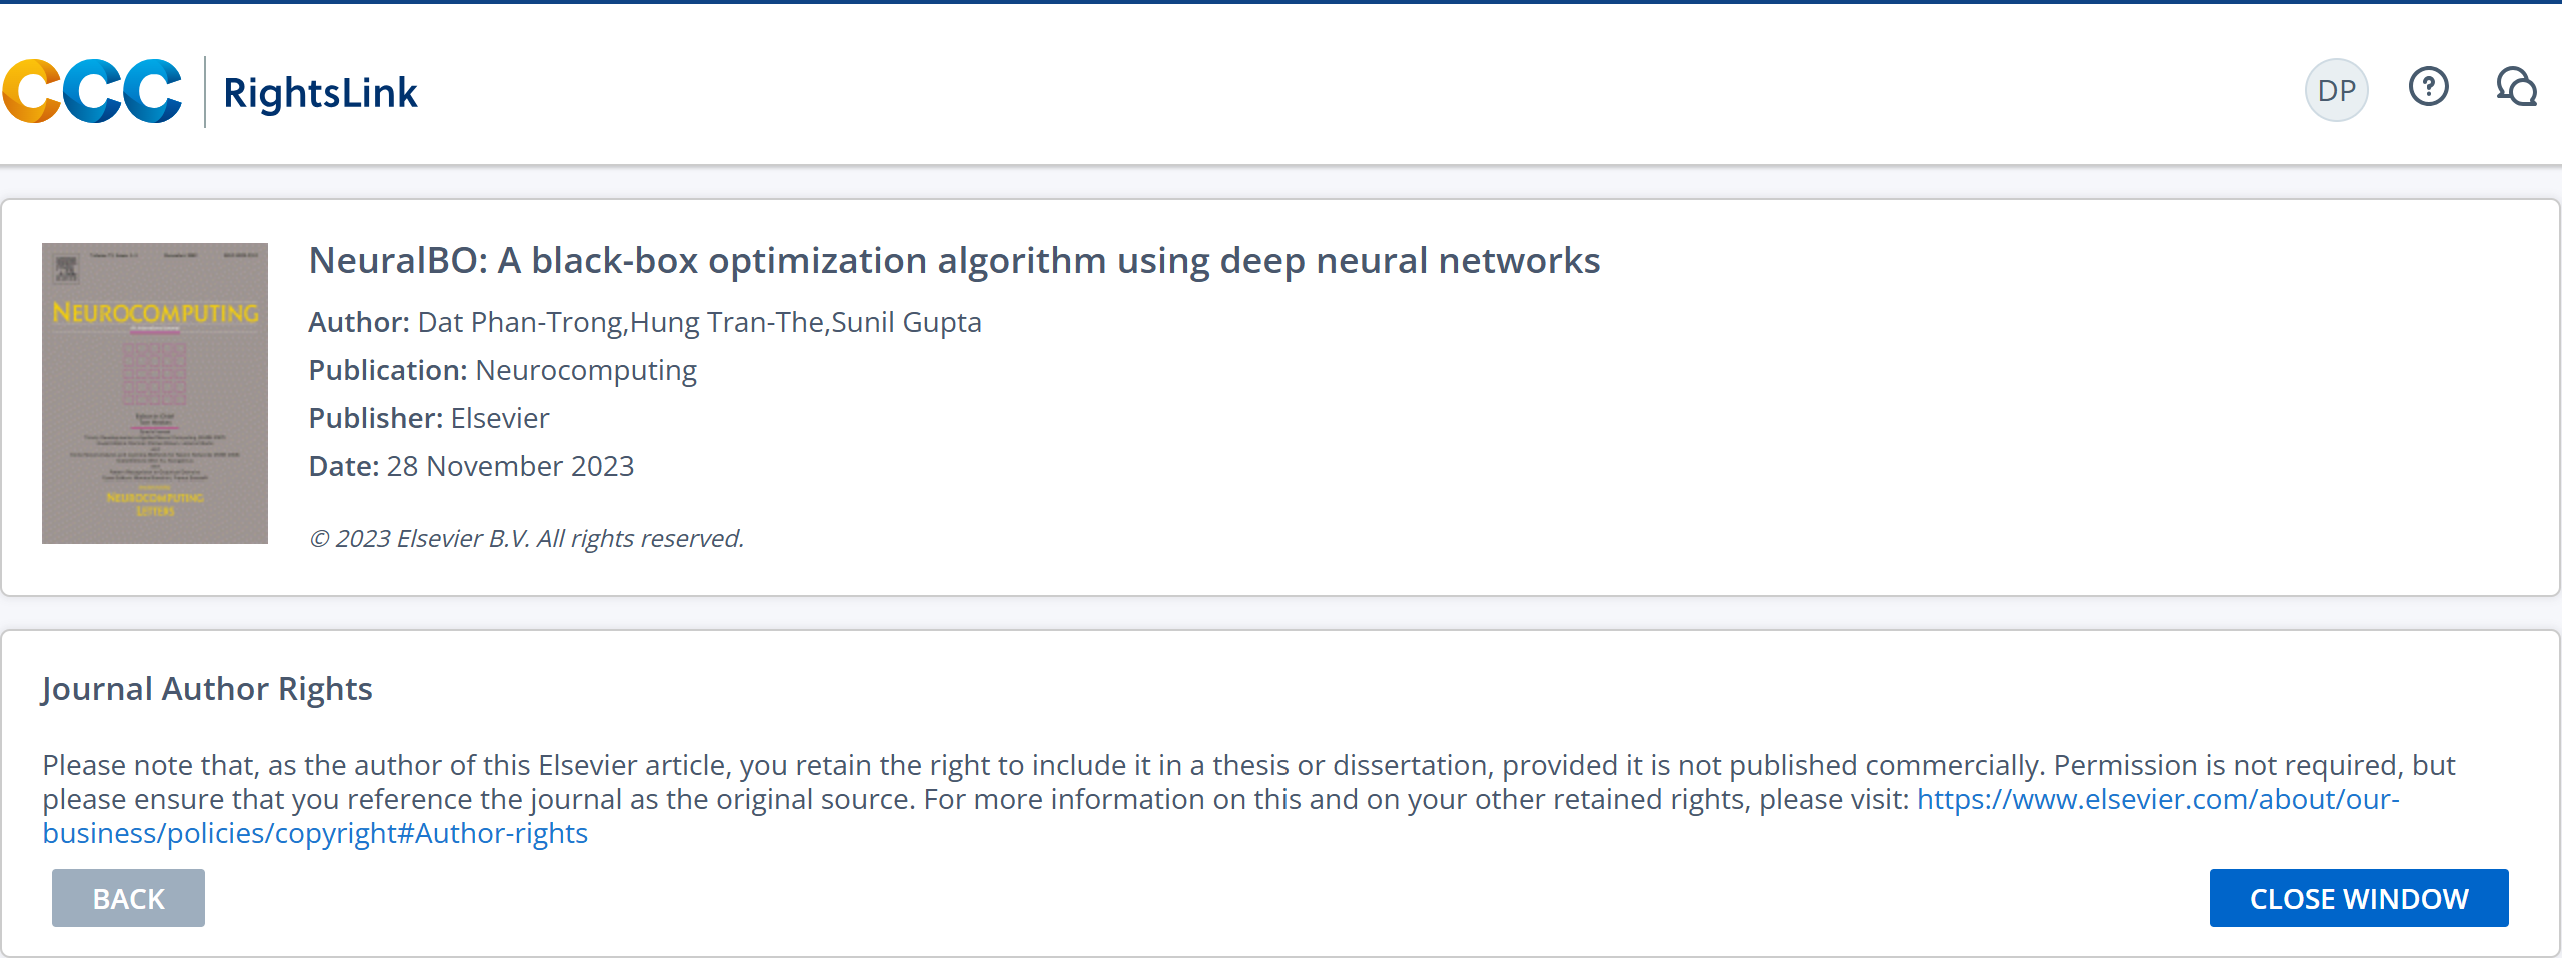
\includegraphics[width=\textwidth]{Figures/Elsvier.png}
\end{figure*}

\section{PINN-BO:}
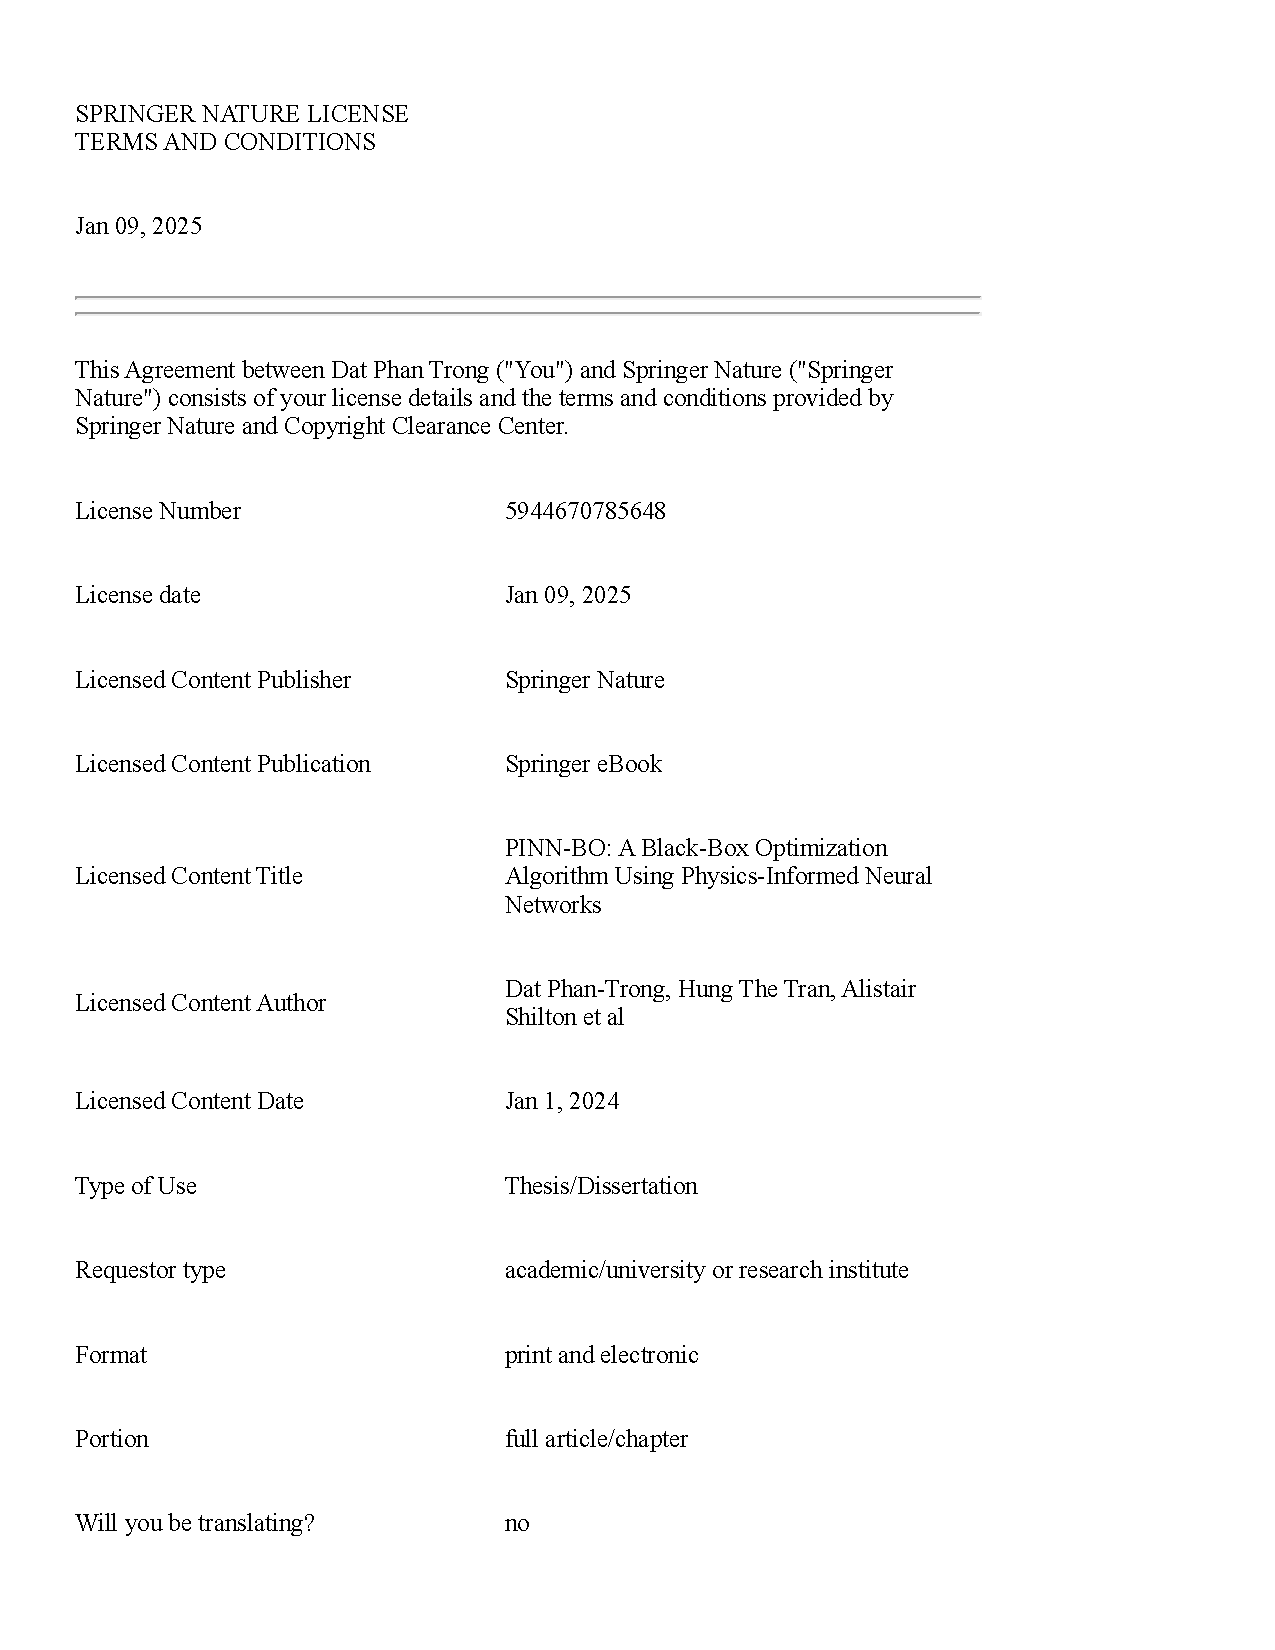
\includepdf[pages=-]{extra_pages/pinnbo_copyrights.pdf}
\end{document}  
